

%% Canadian Association of Physicists
%%----------------------------------------

%% NOTE: exams are formatted so options are on rows, not columns.
%% NOTE: each option is indidivually punctuated
%% NOTE: queens english, not american


%% Their are 520 - 1 multiple-choice questions


%% CAP High School Prize Examinations
%%----------------------------------------


%% Completed Exams:
%% 1995, 1996, 1997, 1998, 1999, 2001
%% 2002, 2003, 2005, 2006
%%----------------------------------------


%% CAP Exam 2015 Part A: Multiple Choice Questions
%%--------------------------------------------------
\element{cap}{ %% CAP-A3
\begin{question}{CAP-A-2015-q01}
    As shown in the picture, a ball is attached to a ceiling and a wall with massless ropes $A$ and $B$.
    Rope $A$ is at angle $\theta$ from the vertical direction, and rope $B$ is horizontal. 
    The system is static. 
    \begin{center}
    \begin{tikzpicture}
        %% ceiling, A
        \draw (1,0) -- (3,0);
        \node[anchor=south,fill,pattern=north east lines,minimum width=2cm, minimum height=0.05cm] at (2,0) {};
        %% wall, B
        \draw (-2,-4) -- (-2,-2);
        \node[anchor=east,fill,pattern=north east lines,minimum width=0.05cm, minimum height=2cm] at (-2,-3) {};
        %% String A and B
        \draw[thick] (0,-3) -- (2,0) node[pos=0.5,anchor=south east] {$A$};
        \draw[thick] (-2,-3) -- (0,-3) node[pos=0.5,anchor=south] {$B$};
        %% Pendulum
        \draw[fill=white!90!black] (0,-3) circle (10pt);
        %% angle
        \draw[dashed] (2,0) -- (2,-1.5);
        \draw[<->] (2,-1) arc (270:238:1) node[pos=0.5,anchor=north] {$\theta$};
    \end{tikzpicture}
    \end{center}
    If rope $B$ is cut,
        what is the ratio of the tension in rope $A$ immediately after it is cut to the tension in $A$ before it is cut?
    \begin{multicols}{2}
    \begin{choices}
        \wrongchoice{$1$}
        \wrongchoice{$\cos\theta$}
        \wrongchoice{$\dfrac{1}{\cos\theta}$}
      \correctchoice{$\cos 2\theta$}
        \wrongchoice{$\cos\theta \sin\theta$}
    \end{choices}
    \end{multicols}
\end{question}
}

\element{cap}{ %% CAP-D2
\begin{question}{CAP-A-2015-q02}
    Consider a circuit made of a wire with uniform resistance in a shape of a circle as shown in the picture. 
    The circle is connected diagonally from point $A$ to point $B$ with the same type of wire. 
    \begin{center}
    \begin{circuitikz}[scale=0.95]
        %% left branch
        \draw[thick] (4,0) to [short,i=$i_0$] (2,0);
        %% center circle
        \draw[thick] (0,0) circle (2cm);
        %% wire AB
        \draw[thick] (240:2) -- (60:2);
        \node[anchor=north east] at  (240:2) {$A$};
        \node[anchor=south west] at  (60:2) {$B$};
        \draw[dashed] (-1,0) -- (1,0);
        \draw[<->] (0.66,0) arc (0:60:0.66) node[pos=0.5,anchor=west] {$\theta$};
        %% right branch
        \draw[thick] (-2,0) to [short,i=$i_0$] (-4,0);
    \end{circuitikz}
    \end{center}
    If the current passing through the circuit is $i_0$,
        what is the current passing through the wire $AB$ as a function of angle $\theta$?
    \begin{multicols}{2}
    \begin{choices}
        \wrongchoice{zero}
        \wrongchoice{$\dfrac{\theta}{\pi-\theta} i_0$}
        \wrongchoice{$\dfrac{\pi-2\theta}{\pi+2} i_0$}
      \correctchoice{$\dfrac{\pi-2\theta}{\pi+4} i_0$}
    \end{choices}
    \end{multicols}
\end{question}
}

\element{cap}{ %% CAP-A3
\begin{question}{CAP-A-2015-q03}
    The following graph represents the speed of a car as a function of time. 
    We know that as the car speeds up there is a friction force with air that can be approximately considered to be proportional to the speed of the car.
    \begin{center}
    \begin{tikzpicture}
        \begin{axis}[
            axis y line=left, 
            axis x line=bottom, 
            axis line style={->},
            xlabel={time},
            xtick={3},
            xticklabels={$t_0$},
            x label style={
                at={(current axis.right of origin)},
                anchor=north east,
            },
            ylabel={velocity},
            ytick=\empty,
            xmin=0,xmax=11,
            ymin=0,ymax=11,
            width=0.8\columnwidth,
            height=0.5\columnwidth,
        ]
        \addplot[line width=1pt] plot coordinates { (0,0) (3,9) (10,9) };
        \addplot[line width=1pt,dashed] plot coordinates { (3,9) (3,0) };
        \end{axis}
    \end{tikzpicture}
    \end{center}
    Which of the following graphs can be the force of the engine as a function of time?
    \begin{multicols}{2}
    \begin{choices}
        \AMCboxDimensions{down=-2.5em}
        \wrongchoice{
            \begin{tikzpicture}
                \begin{axis}[
                    axis y line=left, 
                    axis x line=bottom, 
                    axis line style={->},
                    xlabel={time},
                    xtick={3},
                    xticklabels={$t_0$},
                    x label style={
                        at={(current axis.right of origin)},
                        anchor=north east,
                    },
                    ylabel={velocity},
                    ytick=\empty,
                    xmin=0,xmax=11,
                    ymin=0,ymax=11,
                    width=1.0\columnwidth,
                ]
                \addplot[line width=1pt] plot coordinates { (0,9) (3,9) };
                \addplot[line width=1pt,dashed] plot coordinates { (3,9) (3,0) };
                \addplot[line width=1pt] plot coordinates { (3,5) (10,5) };
                \end{axis}
            \end{tikzpicture}
        }
        \wrongchoice{
            \begin{tikzpicture}
                \begin{axis}[
                    axis y line=left, 
                    axis x line=bottom, 
                    axis line style={->},
                    xlabel={time},
                    xtick={3},
                    xticklabels={$t_0$},
                    x label style={
                        at={(current axis.right of origin)},
                        anchor=north east,
                    },
                    ylabel={velocity},
                    ytick=\empty,
                    xmin=0,xmax=11,
                    ymin=0,ymax=11,
                    width=1.0\columnwidth,
                ]
                \addplot[line width=1pt] plot coordinates { (0,3) (3,9) };
                \addplot[line width=1pt,dashed] plot coordinates { (3,9) (3,0) };
                \addplot[line width=1pt] plot coordinates { (3,2) (10,2) };
                \end{axis}
            \end{tikzpicture}
        }
        %% ANS is C
        \correctchoice{
            \begin{tikzpicture}
                \begin{axis}[
                    axis y line=left, 
                    axis x line=bottom, 
                    axis line style={->},
                    xlabel={time},
                    xtick={3},
                    xticklabels={$t_0$},
                    x label style={
                        at={(current axis.right of origin)},
                        anchor=north east,
                    },
                    ylabel={velocity},
                    ytick=\empty,
                    xmin=0,xmax=11,
                    ymin=0,ymax=11,
                    width=1.0\columnwidth,
                ]
                \addplot[line width=1pt] plot coordinates { (0,3) (3,9) };
                \addplot[line width=1pt,dashed] plot coordinates { (3,9) (3,0) };
                \addplot[line width=1pt] plot coordinates { (3,6) (10,6) };
                \end{axis}
            \end{tikzpicture}
        }
        \wrongchoice{
            \begin{tikzpicture}
                \begin{axis}[
                    axis y line=left, 
                    axis x line=bottom, 
                    axis line style={->},
                    xlabel={time},
                    xtick={3},
                    xticklabels={$t_0$},
                    x label style={
                        at={(current axis.right of origin)},
                        anchor=north east,
                    },
                    ylabel={velocity},
                    ytick=\empty,
                    xmin=0,xmax=11,
                    ymin=0,ymax=11,
                    width=1.0\columnwidth,
                ]
                \addplot[line width=1pt,domain=0:3] { 3 + 0.66 * x * x };
                \addplot[line width=1pt,dashed] plot coordinates { (3,9) (3,0) };
                \addplot[line width=1pt] plot coordinates { (3,6) (10,6) };
                \end{axis}
            \end{tikzpicture}
        }
        \wrongchoice{
            \begin{tikzpicture}
                \begin{axis}[
                    axis y line=left, 
                    axis x line=bottom, 
                    axis line style={->},
                    xlabel={time},
                    xtick={3},
                    xticklabels={$t_0$},
                    x label style={
                        at={(current axis.right of origin)},
                        anchor=north east,
                    },
                    ylabel={velocity},
                    ytick=\empty,
                    xmin=0,xmax=11,
                    ymin=0,ymax=11,
                    width=1.0\columnwidth,
                ]
                \addplot[line width=1pt,domain=0:3] { 3 + 0.66 * x * x };
                \addplot[line width=1pt,dashed] plot coordinates { (3,9) (3,0) };
                \addplot[line width=1pt] plot coordinates { (3,3) (10,3) };
                \end{axis}
            \end{tikzpicture}
        }
    \end{choices}
    \end{multicols}
\end{question}
}

\element{cap}{ %% CAP-??
\begin{question}{CAP-A-2015-q04}
    If electromagnetic radiation with intensity $I$ (power per unit area) is absorbed by a surface,
        it exerts a pressure on the surface that is given by $\frac{I}{c}\cos\theta$,
        where $c$ is the speed of light and $\theta$ is the angle the light rays hit the surface relative to a direction perpendicular to the surface. 
    The Sun has a radiation power of $P=\SI{3.9e26}{\watt}$. 
    The absorption of sunlight by Earth causes a force on Earth that pushes it away from the Sun. 
    Which of the following is closest to the magnitude of this force?
    \begin{multicols}{2}
    \begin{choices}
        \wrongchoice{\SI{e7}{\newton}}
      \correctchoice{\SI{e9}{\newton}}
        \wrongchoice{\SI{e11}{\newton}}
        \wrongchoice{\SI{e13}{\newton}}
    \end{choices}
    \end{multicols}
\end{question}
}

\element{cap}{ %% CAP-??
\begin{question}{CAP-A-2015-q05}
    As shown in the picture a cylinder with volumetric thermal expansion coefficient of $\beta_c=\SI{3e-6}{\per\degreeCelsius}$ is completely submerged and floating in a fluid at the temperature \SI{50}{\degreeCelsius}.
    \emph{Please Note:} not drawn, to scale.
    \begin{center}
    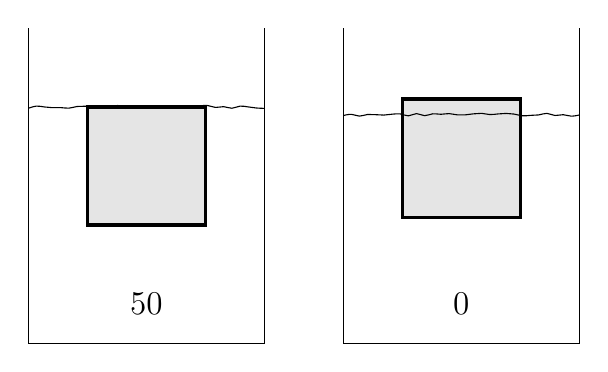
\begin{tikzpicture}
        %% 50 degrees
        \begin{scope}[xshift=-2cm]
            \draw (-1.5,4) -- (-1.5,0) --  (1.5,0) -- (1.5,4);
            \draw[very thick,fill=white!90!black] (-0.75,3) rectangle (0.75,1.5);
            \draw plot [smooth,tension=0.7,samples=30,domain={-1.5:1.5}] (\x,3 + 0.02*rand);
            \node[anchor=center,font=\large] at (0,0.5) {\SI{50}{\degreeCelsius}};
        \end{scope}
        %% 0 degrees
        \begin{scope}[xshift=+2cm]
            \draw (-1.5,4) -- (-1.5,0) --  (1.5,0) -- (1.5,4);
            \draw[very thick,fill=white!90!black] (-0.75,3.1) rectangle (0.75,1.6);
            \draw plot [smooth,tension=0.7,samples=30,domain={-1.5:1.5}] (\x,2.9 + 0.02*rand);
            \node[anchor=center,font=\large] at (0,0.5) {\SI{0}{\degreeCelsius}};
        \end{scope}
    \end{tikzpicture}
    \end{center}
    The fluid has volumetric thermal expansion coefficient of $\beta_f=\SI{3e-5}{\per\degreeCelsius}$.
    If we cool down the cylinder and the fluid to \SI{0}{\degreeCelsius} what percentage of the cylinder's height will be out of the fluid?
    \begin{multicols}{2}
    \begin{choices}
      \correctchoice{\SI{0.39}{\percent}}
        \wrongchoice{\SI{0.42}{\percent}}
        \wrongchoice{\SI{0.78}{\percent}}
        \wrongchoice{\SI{0.84}{\percent}}
    \end{choices}
    \end{multicols}
\end{question}
}

\element{cap}{ %% CAP-??
\begin{question}{CAP-A-2015-q06}
    %% NOTE: the meter was defined as 1/1e6 the distance from the equator to the pole
    The amount of sunlight absorbed by the Earth's atmosphere is approximately proportional to the length of air through which it travels to reach to the Earth.
    Which of the following is closest to the ratio of the absorption of sunlight during sunset relative to the absorption when the Sun is exactly at the center of the sky?
    The effective height of the atmosphere is about \SI{10}{\kilo\meter}.
    \begin{multicols}{4}
    \begin{choices}
        \wrongchoice{22}
      \correctchoice{36}
        \wrongchoice{45}
        \wrongchoice{64}
    \end{choices}
    \end{multicols}
\end{question}
}

\element{cap}{ %% CAP-XX
\begin{question}{CAP-A-2015-q07}
    A beam of red light is made up of a stream of photons. 
    The size of dots represents the photon energy,
        and the spacing represents the spatial distribution between photons.
    \begin{center}
    \begin{tikzpicture}
        %% NOTE: TODO: tikz draw
    \end{tikzpicture}
    \end{center}
    If we use photons of half the wavelength of red light,
        keeping the intensity constant,
        what should the stream look like?
    \begin{choices}
        %% NOTE: ANS is C
        \wrongchoice{
            \begin{tikzpicture}
                %% NOTE: TODO: draw tikz
            \end{tikzpicture}
        }
    \end{choices}
\end{question}
}

\element{cap}{ %% CAP-??
\begin{question}{CAP-A-2015-q08}
    To paint the surface of a solid metal sculpture we need 100 buckets of paint. 
    If we melt the sculpture and create 1000 smaller but otherwise identical sculptures,
        how many buckets of paint are needed to paint the surface of all 1000 small sculptures? 
    Assume that the original and the smaller sculptures are all solid with no cavity inside.
    \begin{multicols}{2}
    \begin{choices}
        \wrongchoice{10}
        \wrongchoice{100}
      \correctchoice{1000}
        \wrongchoice{10000}
    \end{choices}
    \end{multicols}
\end{question}
}

\element{cap}{
\begin{question}{CAP-A-2015-q09}
    A person is standing on a platform that is sliding down the hill as shown in the picture. 
    \begin{center}
    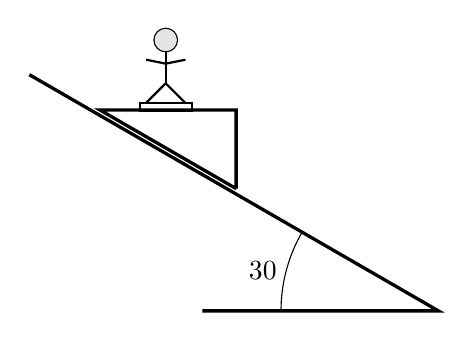
\begin{tikzpicture}
        %% incline
        \draw[very thick] (-3,0) -- (0,0) -- (150:6);
        \draw (-2,0) arc (180:150:2) node[pos=0.5,anchor=east] {\ang{30}};
        %% platform
        \draw[very thick] (60:0.06) ++ (150:3) -- ++(150:2) -- ++(0:1.73) -- ++(270:1);
        %% person
        \begin{scope}[anchor=south,shift={(150:4)},yshift=0.64cm]
            \draw[thick] (0,0.25) -- (0,0.75);
            %% Legs
            \draw[thick] (0,0.25) -- (-0.25,0);
            \draw[thick] (0,0.25) -- (+0.25,0);
            %% Arms
            \draw[thick] (0,0.50) -- (-0.25,0.55);
            \draw[thick] (0,0.50) -- (+0.25,0.55);
            %% Head
            \draw[fill=white!90!black] (0,0.80) circle (0.15cm);
            %% scale
            \draw[thick] (-0.33,0) rectangle (0.33,-0.1);
        \end{scope}
    \end{tikzpicture}
    \end{center}
    The slope of the hill is \ang{30} with respect to the horizontal. 
    The person is standing on a scale positioned on the surface of the platform and the scale is reading only \SI{150}{\pound} while his real weight is \SI{160}{\pound}. 
    Which of the following is the coefficient of kinetic friction between the platform and the slope?
    \begin{multicols}{2}
    \begin{choices}
        \wrongchoice{$\dfrac{\sqrt{3}}{2}$}
      \correctchoice{$\dfrac{\sqrt{3}}{4}$}
        \wrongchoice{$\dfrac{\sqrt{3}}{3}$}
        \wrongchoice{$\dfrac{\sqrt{2}}{3}$}
        \wrongchoice{there is not enough information to calculate the friction coefficient.}
    \end{choices}
    \end{multicols}
\end{question}
}

\element{cap}{ %% CAP-C3
\begin{question}{CAP-A-2015-q10}
    A constant amount of ideal gas, at the temperature $T_0$,
        undergoes a process that changes its pressure from $P_0$ to $2P_0$.
    Then its volume is increased from $V_0$ to $3V_0$ at a constant pressure,
        as shown on the $PV$ diagram:
    \begin{center}
    \begin{tikzpicture}
        \begin{axis}[
            axis y line=left, 
            axis x line=bottom, 
            axis line style={->},
            xlabel={volume},
            xtick={0,1,2,3},
            xticklabels={0,$V_0$,$2V_0$,$3V_0$},
            ylabel={pressure},
            ytick={0,1,2},
            yticklabels={0,$p_0$,$2p_0$},
            xmin=0,xmax=3.5,
            ymin=0,ymax=2.5,
            width=0.8\columnwidth,
            height=0.5\columnwidth,
        ]
        \addplot[line width=1pt,mark=*] plot coordinates { (1,1) (1,2) (3,2) };
        \node[anchor=west] at (axis cs:1,1) {1};
        \node[anchor=south] at (axis cs:1,2) {2};
        \node[anchor=south] at (axis cs:3,2) {3};
        \draw[dashed] (axis cs:1,0) -- (axis cs:1,1);
        \draw[dashed] (axis cs:0,1) -- (axis cs:1,1);
        \draw[dashed] (axis cs:0,2) -- (axis cs:1,2);
        \draw[dashed] (axis cs:3,0) -- (axis cs:3,2);
        \end{axis}
    \end{tikzpicture}
    \end{center}
    Which of the $PT$ diagrams below correctly reflects these processes:
    \begin{choices}
        \AMCboxDimensions{down=-4.5em}
        \wrongchoice{
            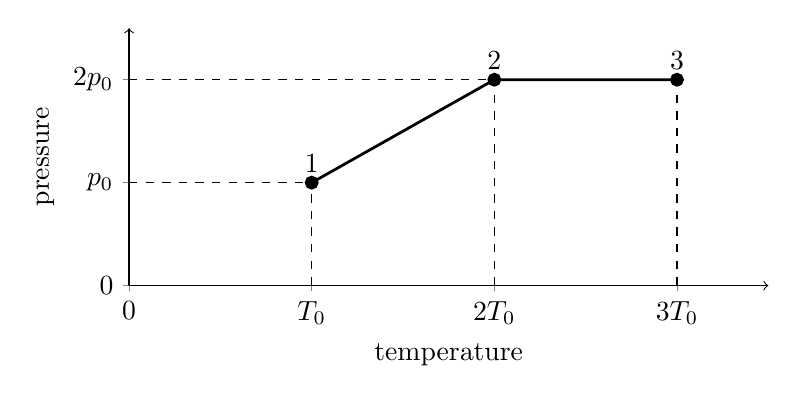
\begin{tikzpicture}
                \begin{axis}[
                    clip=false,
                    axis y line=left, 
                    axis x line=bottom, 
                    axis line style={->},
                    xlabel={temperature},
                    xtick={0,1,2,3},
                    xticklabels={0,$T_0$,$2T_0$,$3T_0$},
                    ylabel={pressure},
                    ytick={0,1,2},
                    yticklabels={0,$p_0$,$2p_0$},
                    xmin=0,xmax=3.5,
                    ymin=0,ymax=2.5,
                    width=0.8\columnwidth,
                    height=0.4\columnwidth,
                ]
                \addplot[line width=1pt,mark=*] plot coordinates { (1,1) (2,2) (3,2) };
                \node[anchor=south] at (axis cs:1,1) {1};
                \node[anchor=south] at (axis cs:2,2) {2};
                \node[anchor=south] at (axis cs:3,2) {3};
                \draw[dashed] (axis cs:0,1) -- (axis cs:1,1);
                \draw[dashed] (axis cs:0,2) -- (axis cs:2,2);
                \draw[dashed] (axis cs:1,0) -- (axis cs:1,1);
                \draw[dashed] (axis cs:2,0) -- (axis cs:2,2);
                \draw[dashed] (axis cs:3,0) -- (axis cs:3,2);
                \end{axis}
            \end{tikzpicture}
        }
        %% ANS is B
        \correctchoice{
            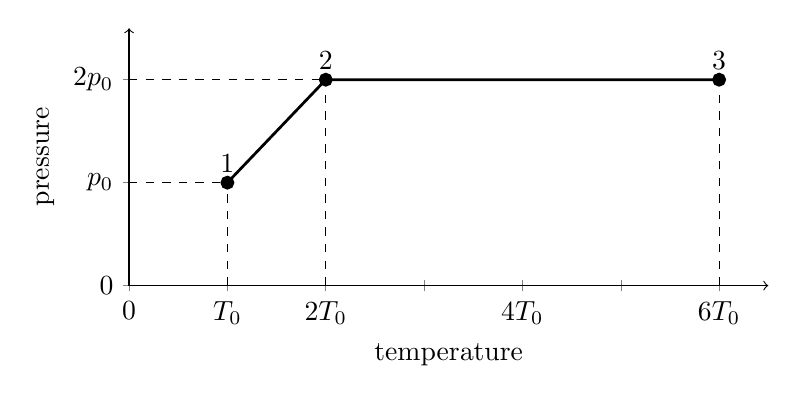
\begin{tikzpicture}
                \begin{axis}[
                    clip=false,
                    axis y line=left, 
                    axis x line=bottom, 
                    axis line style={->},
                    xlabel={temperature},
                    xtick={0,1,2,3,4,5,6},
                    xticklabels={0,$T_0$,$2T_0$,,$4T_0$,,$6T_0$},
                    ylabel={pressure},
                    ytick={0,1,2},
                    yticklabels={0,$p_0$,$2p_0$},
                    xmin=0,xmax=6.5,
                    ymin=0,ymax=2.5,
                    width=0.8\columnwidth,
                    height=0.4\columnwidth,
                ]
                \addplot[line width=1pt,mark=*] plot coordinates { (1,1) (2,2) (6,2) };
                \node[anchor=south] at (axis cs:1,1) {1};
                \node[anchor=south] at (axis cs:2,2) {2};
                \node[anchor=south] at (axis cs:6,2) {3};
                \draw[dashed] (axis cs:0,1) -- (axis cs:1,1);
                \draw[dashed] (axis cs:0,2) -- (axis cs:2,2);
                \draw[dashed] (axis cs:1,0) -- (axis cs:1,1);
                \draw[dashed] (axis cs:2,0) -- (axis cs:2,2);
                \draw[dashed] (axis cs:6,0) -- (axis cs:6,2);
                \end{axis}
            \end{tikzpicture}
        }
        \wrongchoice{
            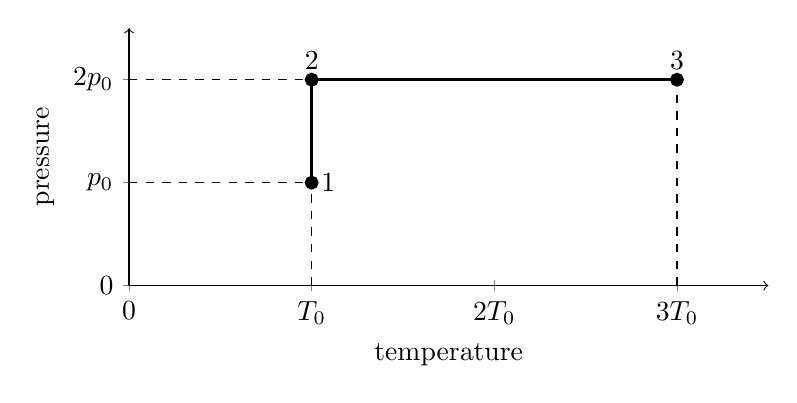
\begin{tikzpicture}
                \begin{axis}[
                    clip=false,
                    axis y line=left, 
                    axis x line=bottom, 
                    axis line style={->},
                    xlabel={temperature},
                    xtick={0,1,2,3},
                    xticklabels={0,$T_0$,$2T_0$,$3T_0$},
                    ylabel={pressure},
                    ytick={0,1,2},
                    yticklabels={0,$p_0$,$2p_0$},
                    xmin=0,xmax=3.5,
                    ymin=0,ymax=2.5,
                    width=0.8\columnwidth,
                    height=0.4\columnwidth,
                ]
                \addplot[line width=1pt,mark=*] plot coordinates { (1,1) (1,2) (3,2) };
                \node[anchor=west] at (axis cs:1,1) {1};
                \node[anchor=south] at (axis cs:1,2) {2};
                \node[anchor=south] at (axis cs:3,2) {3};
                \draw[dashed] (axis cs:0,1) -- (axis cs:1,1);
                \draw[dashed] (axis cs:0,2) -- (axis cs:1,2);
                \draw[dashed] (axis cs:1,0) -- (axis cs:1,1);
                \draw[dashed] (axis cs:3,0) -- (axis cs:3,2);
                \end{axis}
            \end{tikzpicture}
        }
        \wrongchoice{
            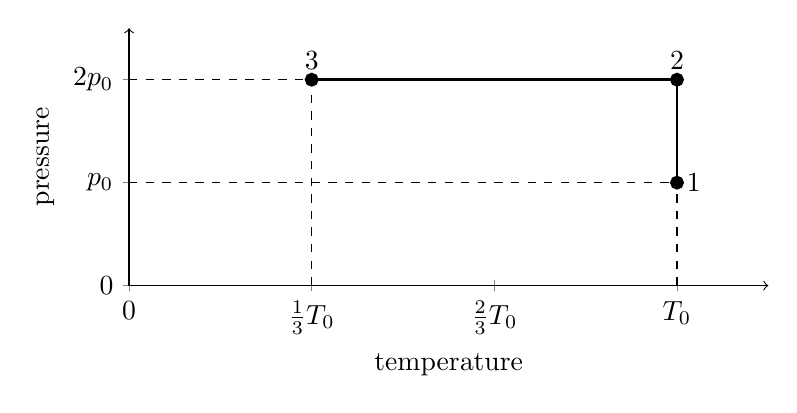
\begin{tikzpicture}
                \begin{axis}[
                    clip=false,
                    axis y line=left, 
                    axis x line=bottom, 
                    axis line style={->},
                    xlabel={temperature},
                    xtick={0,1,2,3},
                    xticklabels={0,$\frac{1}{3}T_0$,$\frac{2}{3}T_0$,$T_0$},
                    ylabel={pressure},
                    ytick={0,1,2},
                    yticklabels={0,$p_0$,$2p_0$},
                    xmin=0,xmax=3.5,
                    ymin=0,ymax=2.5,
                    width=0.8\columnwidth,
                    height=0.4\columnwidth,
                ]
                \addplot[line width=1pt,mark=*] plot coordinates { (1,2) (3,2) (3,1) };
                \node[anchor=west] at (axis cs:3,1) {1};
                \node[anchor=south] at (axis cs:3,2) {2};
                \node[anchor=south] at (axis cs:1,2) {3};
                \draw[dashed] (axis cs:0,1) -- (axis cs:3,1);
                \draw[dashed] (axis cs:0,2) -- (axis cs:1,2);
                \draw[dashed] (axis cs:1,0) -- (axis cs:1,2);
                \draw[dashed] (axis cs:3,0) -- (axis cs:3,1);
                \end{axis}
            \end{tikzpicture}
        }
    \end{choices}
\end{question}
}

\element{cap}{ %% cap-A7
\begin{question}{CAP-A-2015-q11}
    A sentence from a book by a famous bestselling author Dan Brown:
    \begin{quote}
        The pilot nodded. 
        ``Altitude sickness. 
        We were at sixty thousand feet. 
        You're thirty percent lighter up there. 
        Lucky we only did a puddle jump. 
        If we'd gone to Tokyo I'd have taken her all the way up a hundred miles. 
        Now that'll get your insides rolling.''
    \end{quote}
    Is the statement correct?
    \begin{choices}[o]
        \wrongchoice{Yes}
      \correctchoice{No, the distance from the surface of the Earth have to be about \SI{1000}{\kilo\meter} for a person to feel \SI{30}{\percent} lighter.}
        \wrongchoice{No, the person will not feel lighter at higher altitude since the upward force of airplanes engine compensates for the lack of gravity.}
        \wrongchoice{No both arguments (b) and (c) are true.}
    \end{choices}
\end{question}
}

\element{cap}{ %% cap-XX
\begin{question}{CAP-A-2015-q12}
    The figure below shows some light rays coming from point $P$ and passing through a lens.
    \begin{center}
    \begin{tikzpicture}
        %% NOTE: TODO: draw tikz
        %% principal axis
        \draw (-3,0) -- (+3,0);
        %% lens
        \draw[very thick] (0,-2) -- (0,2);
        %% point P
        \draw[ultra thick,->] (-2,0) -- (-2,1) node[anchor=south] {$P$};
        %% Ray diagram
        %\draw[thick,postaction={decorate},decoration={markings, mark=at position .25 with {\arrowreversed{latex}}}] (-2,1) -- (0,1);
        \draw[thick,postaction={decorate},decoration={markings, mark=at position 0.5 with {\arrow{latex}}}] (-2,1) -- (0,1);
    \end{tikzpicture}
    \end{center}
    Which of the distances shown in the diagram below corresponds to the focal length of this lens?
    \begin{center}
    \begin{tikzpicture}
        %% NOTE: TODO: draw tikz
    \end{tikzpicture}
    \end{center}
    \begin{multicols}{4}
    \begin{choices}
        %% NOTE: move each into option??
        \wrongchoice{1}
        \wrongchoice{2}
      \correctchoice{3}
        \wrongchoice{4}
    \end{choices}
    \end{multicols}
\end{question}
}

\element{cap}{ %% cap-A1
\begin{question}{CAP-A-2015-q13}
    A passenger of a train that is moving with the speed of \SI{25}{\meter\per\second} sees from his seat far from a window that it takes 6 seconds for another train to pass the window completely. 
    If the length of the second train is \SI{300}{\meter} and it is going in the opposite direction,
        what is its velocity?
    \begin{multicols}{3}
    \begin{choices}
        \wrongchoice{\SI{15}{\meter\per\second}}
        \wrongchoice{\SI{20}{\meter\per\second}}
      \correctchoice{\SI{25}{\meter\per\second}}
        \wrongchoice{\SI{30}{\meter\per\second}}
        \wrongchoice{\SI{35}{\meter\per\second}}
    \end{choices}
    \end{multicols}
\end{question}
}

\element{cap}{ %% cap-B2
\begin{question}{CAP-A-2015-q14}
    An observer is running toward a mirror with a speed of \SI{15}{\kilo\meter\per\hour},
        and the mirror is moving toward the observer with a speed of \SI{10}{\kilo\meter\per\hour}. 
    What is the relative speed with which the observer sees his image approaching him?
    \begin{multicols}{3}
    \begin{choices}
        \wrongchoice{\SI{10}{\kilo\meter\per\hour}}
        \wrongchoice{\SI{20}{\kilo\meter\per\hour}}
        \wrongchoice{\SI{25}{\kilo\meter\per\hour}}
        \wrongchoice{\SI{30}{\kilo\meter\per\hour}}
      \correctchoice{\SI{50}{\kilo\meter\per\hour}}
    \end{choices}
    \end{multicols}
\end{question}
}

\element{cap}{ %% cap-C2
\begin{question}{CAP-A-2015-q15}
    Three identical closed containers are filled with gases at the same temperature. 
    Container $A$ is filled with \SI{64}{\gram} of oxygen,
        container $B$ is filled with \SI{84}{\gram} of nitrogen,
        and container $C$ is filled with \SI{8}{\gram} of hydrogen. 
    Which is the correct ranking of the pressures in the containers?
    \begin{multicols}{2}
    \begin{choices}
        \wrongchoice{$P_A > P_B > P_C$}
        \wrongchoice{$P_A > P_C > P_B$}
        \wrongchoice{$P_A < P_C < P_B$}
      \correctchoice{$P_A < P_B < P_C$}
        \wrongchoice{$P_A = P_B > P_C$}
    \end{choices}
    \end{multicols}
\end{question}
}

\element{cap}{ %% cap-A4
\begin{question}{CAP-A-2015-q16}
    A ball is placed on a massless spring that is held at an angle of $\theta$ with respect to the horizontal. 
    The spring is then compressed a distance of $x$ and released. 
    When the ball reaches the maximum height of its trajectory,
        it is traveling at a speed $v$.
    Then a different ball, weighing four times as much as the first,
        is placed on the spring which is still at an angle $\theta$. 
    The spring is again compressed a distance $x$ and released. 
    Compared to the first ball, the second ball reaches a maximum height that is:
    \begin{choices}
        \wrongchoice{$\sin^2\theta$ times as high.}
      \correctchoice{$\dfrac{1}{4}$ times as high.}
        \wrongchoice{$\dfrac{v^2 g}{x}$ times as high.}
        \wrongchoice{4 times higher.}
    \end{choices}
\end{question}
}

\element{cap}{ %% cap-XX
\begin{question}{CAP-A-2015-q17}
    A laser beam propagating in glass (shown in white)
        hits the rectangular gap filled with air (shown in gray).
    \begin{center}
    \begin{tikzpicture}
        %% NOTE: TODO: tikz draw
    \end{tikzpicture}
    \end{center}
    Which line shown on the figure below represents correct path of the beam?
    \begin{multicols}{4}
    \begin{choices}
        \wrongchoice{1}
        \wrongchoice{2}
        \wrongchoice{3}
      \correctchoice{4}
    \end{choices}
    \end{multicols}
\end{question}
}

\element{cap}{ %% cap-B2
\begin{question}{CAP-A-2015-q18}
    A parallel beam of light of frequency \SI{6.9e14}{\hertz} enters a glass plate with an index of refraction $n=1.5$.
    The frequency of light in the glass is:
    \begin{multicols}{2}
    \begin{choices}
        \wrongchoice{\SI{4.6e14}{\hertz}}
      \correctchoice{\SI{6.9e14}{\hertz}}
        \wrongchoice{\SI{10.36e14}{\hertz}}
        \wrongchoice{\SI{13.8e14}{\hertz}}
    \end{choices}
    \end{multicols}
\end{question}
}

\element{cap}{ %% cap-??
\begin{question}{CAP-A-2015-q19}
    Students are watching a science fiction movie where the blood spilled during a battle on the a spaceship with its engines turned off form spheres floating in air.
    The students think it is unphysical.
    \begin{choices}
        \wrongchoice{The students are right, because the blood should not form spheres.}
        \wrongchoice{The students are wrong, because in free fall the liquid should form into spheres due to atmospheric pressure.}
      \correctchoice{The students are wrong, because in free fall the liquid should form the spheres due to the surface tension.}
        \wrongchoice{The students are right, because the gravitational forces should immediately pull the blood toward the walls or other objects on the ship.}
    \end{choices}
\end{question}
}

\element{cap}{ %% cap-E3
\begin{question}{CAP-A-2015-q20}
    Unstable elementary particles are produced traveling at $v=0.6c$ with respect to an observer in a laboratory. 
    These particles have a typical intrinsic lifetime of \SI{100}{\nano\second}.
    In the frame of the observer,
        how long will the particles typically last before decaying?
    \begin{choices}
        \wrongchoice{They won't decay while moving}
        \wrongchoice{\SI{100}{\nano\second}}
      \correctchoice{\SI{125}{\nano\second}}
        \wrongchoice{\SI{175}{\nano\second}}
        \wrongchoice{\SI{80}{\nano\second}}
    \end{choices}
\end{question}
}

\element{cap}{ %% cap-XX
\begin{question}{CAP-A-2015-q21}
    A charged moving object enters a volume where a uniform field is present. 
    After some time the object moves in a circular orbit. 
    Which field was present in this area?
    %% NOTE: questionmult: Which fields could be present in this area?
    \begin{choices}[o]
        \wrongchoice{gravitational}
      \correctchoice{magnetic}
        \wrongchoice{electrostatic}
        \wrongchoice{both (a) or (c) are possible}
        \wrongchoice{both (b) or (c) are possible}
    \end{choices}
\end{question}
}

\element{cap}{ %% cap-B4
\begin{question}{CAP-A-2015-q22}
    Students are watching a science fiction movie where the crew of one spaceship watches an explosion on the other spaceship. 
    After a short time interval the crew hear the sound of the explosion. 
    The students think it is unphysical.
    \begin{choices}
        \wrongchoice{The students are right, because there should be no delay: the sound propagates in vacuum at the speed of light.}
        \wrongchoice{The students are wrong. The science adviser of the movie made it according to the laws of physics.}
        \wrongchoice{The students are right, because the steel body of the spaceship blocks the sound}
      \correctchoice{The students are right, because sound cannot propagate in the region between the spaceships}
    \end{choices}
\end{question}
}

\element{cap}{ %% cap-XX
\begin{question}{CAP-A-2015-q23}
    A beam of electrons is sent through a small hole in a piece of foil. 
    The places where the electrons hit on a distant screen are recorded. 
    \begin{center}
    \begin{tikzpicture}
        %% NOTE: TODO: tikz draw
    \end{tikzpicture}
    \end{center}
    If we make the hole smaller,
        the region where the electrons are hitting the screen will be:
    \begin{multicols}{3}
    \begin{choices}
      \correctchoice{bigger}
        \wrongchoice{the same}
        \wrongchoice{smaller}
    \end{choices}
    \end{multicols}
\end{question}
}

\element{cap}{ %% cap-A7
\begin{question}{CAP-A-2015-q24}
    An astronaut takes a pendulum up to the International Space Station (ISS). 
    The ISS orbits \SI{330}{\kilo\meter} above the surface of the Earth. 
    The radius of the Earth is \SI{6371}{\kilo\meter}. 
    Compared to when it is at ground level,
        the pendulum on the ISS swings with a period that is:
    \begin{choices}
        \wrongchoice{\num{49.3e-3} times as long.}
        \wrongchoice{0.95 times as long.}
        \wrongchoice{1.05 times longer.}
        \wrongchoice{20.3 times longer.}
      \correctchoice{The pendulum does not swing on the ISS.}
    \end{choices}
\end{question}
}

\element{cap}{ %% cap-E3
\begin{question}{CAP-A-2015-q25}
    Two objects, $A$ and $B$,
        appear to be the same length in a reference frame when $A$ is stationary and $B$ is moving with speed $\frac{3}{5} c$ along its length. 
    In the frame of reference where $B$ is stationary and $A$ is moving,
        what is the ratio of their lengths?
    \begin{choices}
        \wrongchoice{\num{49.3e-3} times as long.}
      \correctchoice{0.95 times as long.}
        \wrongchoice{1.05 times longer.}
        \wrongchoice{20.3 times longer.}
        \wrongchoice{The pendulum does not swing on the ISS.}
    \end{choices}
\end{question}
}


%% CAP Exam 2014 Part A: Multiple Choice Questions
%%--------------------------------------------------
\element{cap}{ %% cap-D2
\begin{questionmult}{CAP-A-2014-q01}
    Consider the electric power dissipation due to resistance in a circuit. 
    Which of the following changes leave the dissipated electric power unchanged?
    \begin{choices}
      \correctchoice{Doubling the voltage and reducing the current by a factor of two.}
      \correctchoice{Doubling the voltage and increasing the resistance by a factor of four.}
      \correctchoice{Doubling the current and reducing the resistance by a factor of four.}
        %\wrongchoice{None of the above.}
        %\wrongchoice{Both (b) and (c) are correct.}
        %\correctchoice{(a),(b) and (c) are correct.}
    \end{choices}
\end{questionmult}
}

\element{cap}{ %% cap-??
\begin{question}{CAP-A-2014-q02}
    A U-shaped glass tube closed at both ends and positioned vertically is partly filled with water. 
    At a certain time the levels of water are different in the two arms of the tube due to a difference in air pressure above each arm. 
    \begin{center}
    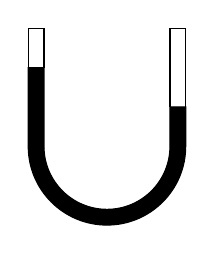
\begin{tikzpicture}
        \draw[fill] (-1,1) -- (-1,0) arc (180:360:1) -- (1,0.5) -- (0.8,0.5) -- (0.8,0) arc (360:180:0.8) -- (-0.8,1) -- cycle;
        \draw (-1,1) -- (-1,1.5) -- (-0.8,1.5) -- (-0.8,1.0);
        \draw (1,0.5) -- (1,1.5) -- (0.8,1.5) -- (0.8,0.5);
    \end{tikzpicture}
    \end{center}
    If there is no temperature change,
        what will happen to the water level on both sides?
    \begin{choices}
        \wrongchoice{The water levels will stay stationary.}
        \wrongchoice{The water levels will equalize rapidly---within seconds.}
      \correctchoice{The water levels will slowly equalize---within days.}
        \wrongchoice{The difference between the levels in each arm will increase.}
    \end{choices}
\end{question}
}

\element{cap}{ %% cap-A7
\begin{question}{CAP-A-2014-q03}
    How does the magnitude of the gravitational force with which the Moon attracts the Earth compare to the magnitude of the gravitational force with which the Earth attracts the Moon?
    \begin{choices}
      \correctchoice{They are equal.}
        \wrongchoice{The first is greater.}
        \wrongchoice{The first is smaller.}
    \end{choices}
\end{question}
}

\element{cap}{ %% cap-A4
\begin{question}{CAP-A-2014-q04}
    The friction force acting on a bicycle is \SI{20}{\newton}. 
    What power does a cyclist need in order to travel at \SI{18}{\kilo\meter\per\hour}?
    \begin{multicols}{2}
    \begin{choices}
        \wrongchoice{\SI{50}{\watt}}
      \correctchoice{\SI{100}{\watt}}
        \wrongchoice{\SI{1800}{\watt}}
        \wrongchoice{\SI{3600}{\watt}}
    \end{choices}
    \end{multicols}
\end{question}
}

\element{cap}{ %% cap-A5
\begin{question}{CAP-A-2014-q05}
    What is the average horizontal force acting on a ball when it elastically bounces off a wall,
        assuming the collision time is \SI{0.1}{\second} and the momentum of the ball before the bounce was \SI{2}{\kilo\gram\meter\per\second},
        perpendicular to the wall?
    \begin{multicols}{2}
    \begin{choices}
        \wrongchoice{\SI{0.2}{\newton}}
        \wrongchoice{\SI{0.4}{\newton}}
      \correctchoice{\SI{40}{\newton}}
        \wrongchoice{\SI{20}{\newton}}
    \end{choices}
    \end{multicols}
\end{question}
}

\element{cap}{ %% cap-XX
\begin{question}{CAP-A-2014-q06}
    A small explosion occurs in a model airplane which rips it into two pieces. 
    The model was flying with velocity $v$ just before the explosion. 
    \begin{center}
    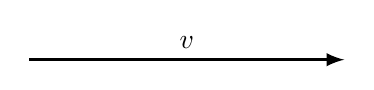
\begin{tikzpicture}
        \draw[very thick,-latex] (0,0) -- (4,0) node[pos=0.5,anchor=south] {$v$};
    \end{tikzpicture}
    \end{center}
    Which combination of $v_1$ and $v_2$ are possible velocities of the two pieces after the explosion?
    \begin{multicols}{2}
    \begin{choices}
        \AMCboxDimensions{down=-0.8cm}
        %% ANS is A
        \correctchoice{
            \begin{tikzpicture}
                \draw[dashed,white!90!black] (0,0) rectangle (3,3);
            \end{tikzpicture}
        }
        \wrongchoice{
            \begin{tikzpicture}
                \draw[dashed,white!90!black] (0,0) rectangle (3,3);
            \end{tikzpicture}
        }
    \end{choices}
    \end{multicols}
\end{question}
}

\element{cap}{ %% cap-D1
\begin{question}{CAP-A-2014-q07}
    Three ping-pong balls are electrically charged and are arranged in the plane of the page in an equilateral triangle as shown below. 
    \begin{center}
    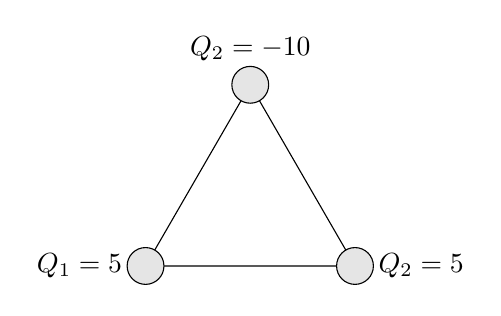
\begin{tikzpicture}[scale=1.33]
        \draw (0,0) -- (1,1.73) -- (2,0) -- cycle;
        \draw[fill=white!90!black] (0,0) circle (5pt) node[anchor=east,xshift=-5pt] {$Q_1=\SI{5}{\micro\coulomb}$};
        \draw[fill=white!90!black] (1,1.73) circle (5pt) node[anchor=south,yshift=5pt] {$Q_2=\SI{-10}{\micro\coulomb}$};
        \draw[fill=white!90!black] (2,0) circle (5pt) node[anchor=west,xshift=5pt] {$Q_2=\SI{5}{\micro\coulomb}$};
    \end{tikzpicture}
    \end{center}
    What is the direction of the force acting on the ping-pong ball charged with $Q_3 = \SI{-10}{\micro\coulomb}$?
    \begin{choices}
        \wrongchoice{Towards the top of the page.}
      \correctchoice{Towards the bottom of the page.}
        \wrongchoice{Towards the left.}
        \wrongchoice{Towards the right.}
        \wrongchoice{Another direction.}
    \end{choices}
\end{question}
}

\element{cap}{ %% cap-D2
\begin{question}{CAP-A-2014-q08}
    In the circuit shown below,
        the resistance $R_1$ is increased. 
    \begin{center}
    \ctikzset{bipoles/length=1.00cm}
    \begin{circuitikz}
        \draw (0,0) to [battery] (4,0) to (4,2) to [R,l=$R_2$] (2,2) to [R,l=$R_1$] (0,2) to (0,0);
    \end{circuitikz}
    \end{center}
    What happens to the magnitude of the potential difference across $R_1$?
    \begin{choices}
      \correctchoice{It increases.}
        \wrongchoice{It decreases.}
        \wrongchoice{It remains the same.}
    \end{choices}
\end{question}
}

\element{cap}{ %% cap-B4
\begin{question}{CAP-A-2014-q09}
    Two identical loudspeakers, placed close to each other,
        are supplied with the same sinusoidal voltage. 
    One can imagine a pattern around the loudspeakers with alternating areas of increased and decreased sound intensity. 
    Which of the actions below will not change the positions of these areas?
    \begin{choices}
        \wrongchoice{Moving one of the speakers.}
      \correctchoice{Changing the amplitude of the voltage.}
        \wrongchoice{Changing the frequency.}
        \wrongchoice{Replacing the air in the room with a gas of a different density.}
    \end{choices}
\end{question}
}

\element{cap}{ %% cap-A7
\begin{question}{CAP-A-2014-q10}
    Two artificial satellites, named Argo and Navis,
        have circular orbits of radii $R$ and $2R$,
        respectively, about the same planet. 
    The orbital speed of Argo is $v$. 
    What is the orbital speed of Navis?
    \begin{multicols}{3}
    \begin{choices}
        \wrongchoice{$\dfrac{v}{2}$}
      \correctchoice{$\dfrac{v}{\sqrt{2}}$}
        \wrongchoice{$v$}
        \wrongchoice{$v\sqrt{2}$}
        \wrongchoice{$2v$}
    \end{choices}
    \end{multicols}
\end{question}
}

\element{cap}{ %% cap-??
\begin{question}{CAP-A-2014-q11}
    When someone drags their fingernails across a chalkboard,
        a terrible high-pitched sound is produced due to small bumps in the chalkboard. 
    Assume these bumps are uniformly spaced by \SI{0.5}{\milli\meter}. 
    Audiologists have determined that humans find sounds in the range of \SI{2}{\kilo\hertz} to \SI{4}{\kilo\hertz} to be very annoying. 
    An evil teacher wants to produce the longest duration continuous sound in this range by dragging her fingernails across the chalkboard. 
    At what speed should she drag her nails to accomplish this?
    \begin{multicols}{2}
    \begin{choices}
        \wrongchoice{\SI{0.28}{\meter\per\second}}
        \wrongchoice{\SI{0.56}{\meter\per\second}}
      \correctchoice{\SI{1.00}{\meter\per\second}}
        \wrongchoice{\SI{2.00}{\meter\per\second}}
    \end{choices}
    \end{multicols}
\end{question}
}

\element{cap}{ %% cap-??
\begin{question}{CAP-A-2014-q12}
    The Hall Effect occurs when both a current and magnetic field are present and perpendicular to each other in a solid. 
    The result is the generation of an electric field and a corresponding potential difference (the Hall voltage) across the width of the solid. 
    Suppose a two-dimensional rectangular material carries a current of \SI{0.5}{\ampere} in the positive $x$ direction and is penetrated by a magnetic field of \SI{1.4}{\milli\tesla} in the negative z direction.
    The number of mobile charges per unit area of the material is \SI{0.2}{\micro\coulomb\per\meter\squared}.
    What is the magnitude of the Hall voltage,
        and the direction of the generated electric field? 
    (Assume a right-handed coordinate system)
    \begin{choices}
        \wrongchoice{\SI{70}{\micro\volt}, negative $y$ direction}
        \wrongchoice{\SI{70}{\micro\volt}, positive $y$ direction}
      \correctchoice{\SI{3.5}{\micro\volt}, negative $y$ direction}
        \wrongchoice{\SI{3.5}{\micro\volt}, positive $y$ direction}
    \end{choices}
\end{question}
}

\element{cap}{ %% cap-E2
\begin{question}{CAP-A-2014-q13}
    Polonium-214 atoms have a mass of \SI{3.55e-22}{\gram} and decay into \ce{^{210}Pb} with a half-life of \SI{160}{\micro\second}. 
    A detector encompassing \SI{1}{\gram} of \ce{^{214}Po} counts the number of \ce{^{210}Pb} daughters produced. 
    An experimentalist rigs an oscillator so that the frequency of electromagnetic radiation it emits matches the frequency of \ce{^{210}Pb} counts measured by detector. 
    After \SI{8}{\milli\second},
        what type of electromagnetic radiation is produced by the oscillator?
    \begin{choices}
      \correctchoice{Radar}
        \wrongchoice{Red light}
        \wrongchoice{Ultra-violet}
        \wrongchoice{X-rays}
    \end{choices}
\end{question}
}

\element{cap}{ %% cap-A4
\begin{question}{CAP-A-2014-q14}
    To submerge a block of wood which is less dense than water,
        one needs to exert a force downward which does a positive amount of work on the block. 
    Which of the following is correct for this situation to occur?
    \begin{choices}
        \wrongchoice{The work done by the external force is stored as potential energy in the block.}
        \wrongchoice{The block is moving downward, therefore its potential energy is decreasing, thus the work done by the external force is all converted to heat, due to friction.}
        \wrongchoice{The work done by external force is all stored as kinetic energy in the block.}
      \correctchoice{The potential energy of the water is increased while the potential energy of the block is decreased.}
        \wrongchoice{The total energy of the block is conserved.}
        \wrongchoice{The total energy of the block and water is conserved.}
    \end{choices}
\end{question}
}

\element{cap}{ %% cap-A1
\begin{question}{CAP-A-2014-q15}
    In 1929, Edwin Hubble discovered that the universe is expanding. 
    He observed that galaxies far away from us are moving away at a speed that is proportional to their distance from us 
        (you can assume the constant of proportionality is time-independent). 
    For a galaxy that obeys Hubble's law,
        which of the following can be the graph of distance (from Earth) versus time? 
    For each plot, $t=0$ corresponds to the present.
    \begin{multicols}{2}
    \begin{choices}
        \AMCboxDimensions{down=-2.5em}
        \wrongchoice{
            \begin{tikzpicture}
                \begin{axis}[
                    axis y line=left, 
                    axis x line=bottom, 
                    axis line style={->},
                    xlabel={time},
                    xtick=\empty,
                    ylabel={distance},
                    ytick=\empty,
                    xmin=0,xmax=11,
                    ymin=0,ymax=11,
                    width=1.0\columnwidth,
                ]
                \addplot[line width=1pt] plot coordinates { (0,2) (10,10) };
                \end{axis}
            \end{tikzpicture}
        }
        %% NOTE: ANS is B
        \correctchoice{
            \begin{tikzpicture}
                \begin{axis}[
                    axis y line=left, 
                    axis x line=bottom, 
                    axis line style={->},
                    xlabel={time},
                    xtick=\empty,
                    ylabel={distance},
                    ytick=\empty,
                    xmin=0,xmax=11,
                    ymin=0,ymax=11,
                    width=1.0\columnwidth,
                ]
                \addplot[line width=1pt,domain=0:10] { 2 + 0.08*x*x };
                \end{axis}
            \end{tikzpicture}
        }
        \wrongchoice{
            \begin{tikzpicture}
                \begin{axis}[
                    axis y line=left, 
                    axis x line=bottom, 
                    axis line style={->},
                    xlabel={time},
                    xtick=\empty,
                    ylabel={distance},
                    ytick=\empty,
                    xmin=0,xmax=11,
                    ymin=0,ymax=11,
                    width=1.0\columnwidth,
                ]
                \addplot[line width=1pt,domain=0:10] { 10 - 0.08*(x-10)*(x-10) };
                \end{axis}
            \end{tikzpicture}
        }
        \wrongchoice{
            \begin{tikzpicture}
                \begin{axis}[
                    axis y line=left, 
                    axis x line=bottom, 
                    axis line style={->},
                    xlabel={time},
                    xtick=\empty,
                    ylabel={distance},
                    ytick=\empty,
                    xmin=0,xmax=11,
                    ymin=0,ymax=11,
                    width=1.0\columnwidth,
                ]
                %\addplot[line width=1pt,domain=0:10] { 2 + exp(x)/2200 };
                \addplot[line width=1pt,domain=0:10] { 2 + 0.0008*x*x*x*x };
                \end{axis}
            \end{tikzpicture}
        }
    \end{choices}
    \end{multicols}
\end{question}
}

\element{cap}{ %% cap-??
\begin{question}{CAP-A-2014-q16}
    Which of the following is closest to the thickness of a piece of paper?
    \begin{multicols}{3}
    \begin{choices}
        \wrongchoice{\SI{e-3}{\meter}}
      \correctchoice{\SI{e-4}{\meter}}
        \wrongchoice{\SI{e-5}{\meter}}
        \wrongchoice{\SI{e-6}{\meter}}
        \wrongchoice{\SI{e-7}{\meter}}
    \end{choices}
    \end{multicols}
\end{question}
}

\element{cap}{ %% cap-??
\begin{question}{CAP-A-2014-q17}
    The paper-folding theorem states that in order to fold something in half,
        it's length must be at least $\pi$ times its thickness. 
    How many times can you fold a standard sheet of printing paper ($\SI{0.216}{\meter}\times\SI{0.279}{\meter}$) if you always fold from the middle of the longer edge?
    \begin{multicols}{4}
    \begin{choices}
        \wrongchoice{5}
        \wrongchoice{6}
      \correctchoice{7}
        \wrongchoice{12}
    \end{choices}
    \end{multicols}
\end{question}
}

\element{cap}{ %% cap-D2
\begin{question}{CAP-A-2014-q18}
    A circuit contains nothing but a battery of voltage $V$ wired to three resistors of resistance $R$. 
    Which of the following cannot be the power dissipated in the circuit
        (assuming negligible resistance for the wires)?
    \begin{multicols}{2}
    \begin{choices}
        \wrongchoice{$P = \dfrac{V^2}{3 R}$}
        \wrongchoice{$P = \dfrac{3 V^2}{R}$}
        \wrongchoice{$P = \dfrac{3 V^2}{2 R}$}
        \wrongchoice{$P = \dfrac{2 V^2}{3 R}$}
      \correctchoice{All of the provided are possible}
    \end{choices}
    \end{multicols}
\end{question}
}

\element{cap}{ %% cap-A7
\begin{question}{CAP-A-2014-q19}
    In a binary star system consisting of two stars of equal mass,
        where is the gravitational potential equal to zero? 
    Assume that for a single star in empty space,
        the potential is zero at infinity.
    \begin{choices}
        \wrongchoice{Exactly halfway between the stars.}
        \wrongchoice{Along a line bisecting the line connecting the stars and perpendicular to the plane of the stars' orbit.}
      \correctchoice{Infinitely far from the stars.}
        \wrongchoice{At any point on a plane bisecting the line connecting the stars and perpendicular to the plane of the stars' orbit.}
    \end{choices}
\end{question}
}

\element{cap}{ %% cap-B3
\begin{question}{CAP-A-2014-q20}
    In Young's double-slit experiment,
        both slits are illuminated by a laser beam and the interference pattern is observed on a screen. 
    If the viewing screen is moving farther from the slits,
        what will happen to the interference pattern?
    \begin{choices}
        \wrongchoice{The pattern gets brighter.}
        \wrongchoice{The pattern gets brighter and the fringes move closer to each other and to the central fringe.}
        \wrongchoice{The pattern gets brighter and the fringes move farther from the central fringe and from each other.}
      \correctchoice{The pattern gets less bright and fringes appear farther apart.}
        \wrongchoice{There is no change in the pattern.}
        \wrongchoice{The pattern becomes unfocused.}
    \end{choices}
\end{question}
}

\element{cap}{ %% cap-A4
\begin{question}{CAP-A-2014-q21}
    A ball is dropped to the Earth from a height of \SI{2}{\meter}.
    Neglecting the air resistance,
        which one of the following graphs represents the kinetic energy of the ball vs. time?
    \begin{multicols}{2}
    \begin{choices}
        \AMCboxDimensions{down=-2.5em}
        \wrongchoice{
            \begin{tikzpicture}
                \begin{axis}[
                    axis y line=left, 
                    axis x line=bottom, 
                    axis line style={->},
                    xlabel={time},
                    xtick=\empty,
                    ylabel={kinetic energy},
                    ytick=\empty,
                    xmin=0,xmax=11,
                    ymin=0,ymax=11,
                    width=1.0\columnwidth,
                ]
                \addplot[line width=1pt] plot coordinates { (0,3) (10,3) };
                \end{axis}
            \end{tikzpicture}
        }
        \wrongchoice{
            \begin{tikzpicture}
                \begin{axis}[
                    axis y line=left, 
                    axis x line=bottom, 
                    axis line style={->},
                    xlabel={time},
                    xtick=\empty,
                    ylabel={kinetic energy},
                    ytick=\empty,
                    xmin=0,xmax=11,
                    ymin=0,ymax=11,
                    width=1.0\columnwidth,
                ]
                \addplot[line width=1pt] plot coordinates { (0,0) (10,10) };
                \end{axis}
            \end{tikzpicture}
        }
        %% ANS is C
        \correctchoice{
            \begin{tikzpicture}
                \begin{axis}[
                    axis y line=left, 
                    axis x line=bottom, 
                    axis line style={->},
                    xlabel={time},
                    xtick=\empty,
                    ylabel={kinetic energy},
                    ytick=\empty,
                    xmin=0,xmax=11,
                    ymin=0,ymax=11,
                    width=1.0\columnwidth,
                ]
                \addplot[line width=1pt,domain=0:10] { 0.1*x*x };
                \end{axis}
            \end{tikzpicture}
        }
        \wrongchoice{
            \begin{tikzpicture}
                \begin{axis}[
                    axis y line=left, 
                    axis x line=bottom, 
                    axis line style={->},
                    xlabel={time},
                    xtick=\empty,
                    ylabel={kinetic energy},
                    ytick=\empty,
                    xmin=0,xmax=11,
                    ymin=0,ymax=11,
                    width=1.0\columnwidth,
                ]
                \addplot[line width=1pt,domain=0:10] { sqrt(10) * sqrt(x) };
                \end{axis}
            \end{tikzpicture}
        }
    \end{choices}
    \end{multicols}
\end{question}
}

\element{cap}{ %% cap-B2
\begin{question}{CAP-A-2014-q22}
    What will happen to the magnitude of the optical power of a lens when it is placed in water ($n=1.33$) compared to its power in the air ($n=1.00$)?
    \begin{choices}
        \wrongchoice{It will increase.}
      \correctchoice{It will decrease.}
        \wrongchoice{It will stay the same.}
        \wrongchoice{It will depend on whether the lens is converging or diverging.}
    \end{choices}
\end{question}
}

\element{cap}{ %% cap-D2
\begin{question}{CAP-A-2014-q23}
    The three electric heaters in the following circuit all have the same resistance. 
    \begin{center}
    \ctikzset{bipoles/length=1.00cm}
    \begin{circuitikz}[]
        \draw (0,0) to [battery] (4,0) to (4,1) to [R,l=$C$] (2,1) to [R,l=$B$] (0,1) to (0,0);
        \draw (4,1) to (4,2) to [R,l=$A$] (0,2) to (0,1);
    \end{circuitikz}
    \end{center}
    Given that the total heat emitted by a heater is proportional to the power dissipated,
        the total heat produced by $B$ and $C$ together,
        compared with the heat produced in $A$, is:
    \begin{choices}
        \wrongchoice{A quarter as much.}
      \correctchoice{Half as much.}
        \wrongchoice{The same.}
        \wrongchoice{Twice as much.}
        \wrongchoice{Four times as much.}
    \end{choices}
\end{question}
}

\element{cap}{ %% cap-A3
\begin{question}{CAP-A-2014-q24}
    A box sits on a horizontal surface that exerts a normal force $N$ on the box. 
    You apply a horizontal force to it and it does not move. 
    If you had applied a force twice as large,
        it still would not have moved. 
    Let $\mu_s$ be the coefficient of static friction of the surface. 
    While you are applying your initial force,
        which of the following is true of the force of friction acting on the box?
    \begin{multicols}{2}
    \begin{choices}
        \wrongchoice{$F_f = 0$}
      \correctchoice{$F_f <    \mu_s N$}
        \wrongchoice{$F_f \leq \mu_s N$}
        \wrongchoice{$F_f =    \mu_s N$}
        \wrongchoice{$F_f \geq \mu_s N$}
        \wrongchoice{$F_f >    \mu_s N$}
    \end{choices}
    \end{multicols}
\end{question}
}

\element{cap}{ %% cap-??
\begin{question}{CAP-A-2014-q25}
    Which of the following is closer to the dimensions of a solar cell panel that can produce enough energy for a family in Vancouver in summer time?
    The following information might be useful:

    %% first piece
    \hspace{1em} The price of residential electricity in British Columbia is approximately 6.90 cents per \si{\kilo\watt\hour}. 
    A typical household's monthly electricity bill is 40 dollars in the summer.

    %% second piece
    \hspace{1em} The power per area from sunlight that reaches the city of Vancouver is about \SI{0.5}{\kilo\watt\per\meter\squared} (averaged over 24 hours) during the period of June-September.
    The efficiency of a typical solar cell is about \SI{20}{\percent}.
    \begin{choices}
        \wrongchoice{$\SI{30}{\centi\meter}\times\SI{30}{\centi\meter}$}
      \correctchoice{$\SI{3}{\meter}\times\SI{3}{\meter}$}
        \wrongchoice{$\SI{30}{\meter}\times\SI{30}{\meter}$}
        \wrongchoice{$\SI{300}{\meter}\times\SI{030}{\meter}$}
        \wrongchoice{The size of the panel must be much bigger than any of these numbers,
            since it is always cloudy in Vancouver and the city does not get enough sunshine!}
    \end{choices}
\end{question}
}


%% CAP Exam 2013 Part A: Multiple Choice Questions
%%--------------------------------------------------
\element{cap}{ %% cap-XX
\begin{question}{CAP-A-2013-q01}
    A small block of mass $m_1$ is released from rest at the top of a curve-shaped,
        frictionless wedge of mass $m_2$ which sits on a frictionless horizontal surface as shown.
    \begin{center}
    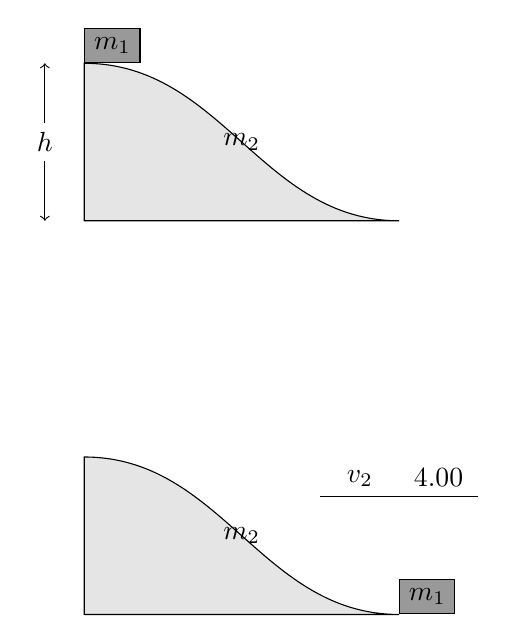
\begin{tikzpicture}
        %% block on top
        \begin{scope}[yshift=+2cm]
            %% wedge, m_2
            \draw[fill=white!90!black] (-2,0) -- (-2,2) to [out=0,in=180] (2,0) --cycle;
            \node[anchor=center] at (0,1) {$m_2$};
            \draw[<->] (-2.5,0) -- (-2.5,2) node[pos=0.5,anchor=center,fill=white] {$h$};
            %% block, m_1
            \node[draw,fill=white!60!black,minimum size=0.25cm,anchor=south west] at (-2,2) {$m_1$};
        \end{scope}
        %% block at bottom
        \begin{scope}[yshift=-3cm]
            %% wedge, m_2
            \draw[fill=white!90!black] (-2,0) -- (-2,2) to [out=0,in=180] (2,0) --cycle;
            \node[anchor=center] at (0,1) {$m_2$};
            \draw (2,1.5) -- ++(180:1) node[pos=0.5,anchor=south] {$v_2$};
            %% block, m_1
            \node[draw,fill=white!60!black,minimum size=0.25cm,anchor=south west] at (2,0) {$m_1$};
            \draw (2,1.5) -- ++(0:1) node[pos=0.5,anchor=south] {\SI{4.00}{\meter\per\second}};
        \end{scope}
    \end{tikzpicture}
    \end{center}
    When the block leaves the wedge its velocity is measured to be \SI{4.00}{\meter\per\second} to the right as shown in the figure. 
    If the mass of the block is doubled to become $2m_1$,
        what can be said about the speed with which it leaves the wedge?
    \begin{choices}
      \correctchoice{Its speed is less than \SI{4.00}{\meter\per\second}}
        \wrongchoice{Its speed is equal to \SI{4.00}{\meter\per\second}}
        \wrongchoice{Its speed is greater than \SI{4.00}{\meter\per\second}}
        \wrongchoice{Not enough information is given.}
    \end{choices}
\end{question}
}

\element{cap}{ %% cap-D1
\begin{question}{CAP-A-2013-q02}
    Consider the electric charges $A$, $B$, $C$ shown in the figure below,
        where $q$ is a positive number. 
    \begin{center}
    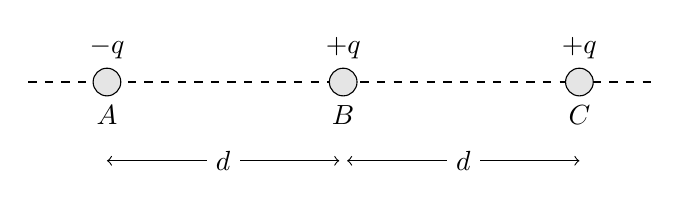
\begin{tikzpicture}
        %% axis
        \draw[dashed] (-4,0) -- (4,0);
        %% charges
        \draw[fill=white!90!black] (-3,0) circle (5pt)
            node[anchor=south,yshift=+5pt] {$-q$}
            node[anchor=north,yshift=-5pt] {$A$};
        \draw[fill=white!90!black] (0,0) circle (5pt)
            node[anchor=south,yshift=+5pt] {$+q$}
            node[anchor=north,yshift=-5pt] {$B$};
        \draw[fill=white!90!black] (3,0) circle (5pt)
            node[anchor=south,yshift=+5pt] {$+q$}
            node[anchor=north,yshift=-5pt] {$C$};
        %% distances
        \draw[<->] (-3,-1) -- (-0.05,-1) node[pos=0.5,anchor=center,fill=white] {$d$};
        \draw[<->] (+3,-1) -- (+0.05,-1) node[pos=0.5,anchor=center,fill=white] {$d$};
    \end{tikzpicture}
    \end{center}
    Which answer correctly describes the magnitude of the net force experienced by the charges?
    \begin{multicols}{2}
    \begin{choices}
        \wrongchoice{$F_A > F_B > F_C$}
        \wrongchoice{$F_A > F_C > F_B$}
      \correctchoice{$F_B > F_A > F_C$}
        \wrongchoice{$F_A = F_B = F_C$}
        \wrongchoice{$F_A > F_B = F_C$}
    \end{choices}
    \end{multicols}
\end{question}
}

\element{cap}{ %% cap-D5
\begin{question}{CAP-A-2013-q03}
    A long, straight wire carries a current that decreases linearly with time. 
    What is the direction of the induced electric field outside the wire?
    \begin{choices}
      \correctchoice{Parallel to the current in the wire, in the same direction.}
        \wrongchoice{Parallel to the current in the wire, in the opposite direction.}
        \wrongchoice{Pointing radially outward from the wire.}
        \wrongchoice{Pointing radially inward toward the wire.}
        \wrongchoice{There is no induced electric field outside the wire.}
    \end{choices}
\end{question}
}

\element{cap}{ %% cap-A3
\begin{question}{CAP-A-2013-q04}
    A car driven at a constant speed turns left. 
    Which force makes the car turn?
    \begin{choices}
      \correctchoice{The force of friction, directed towards the left.}
        \wrongchoice{The force of friction, directed towards the right.}
        \wrongchoice{The force with which the driver is turning the steering wheel, directed towards the left.}
        \wrongchoice{The force with which the driver is turning the steering wheel, directed towards the right.}
    \end{choices}
\end{question}
}

\element{cap}{ %% cap-A3
\begin{question}{CAP-A-2013-q05}
    A cyclist stops pedaling at a velocity $v=\SI{36}{\kilo\meter\per\hour}$ and notices that her bike keeps moving for $d=\SI{500}{\meter}$ before it stops. 
    The total mass of the bike, the biker and her camping equipment is $m=\SI{100}{\kilo\gram}$.
    What is the average combined force on the bicycle due to friction and drag?
    \begin{multicols}{2}
    \begin{choices}
      \correctchoice{\SI{10}{\newton}}
        \wrongchoice{\SI{20}{\newton}}
        \wrongchoice{\SI{130}{\newton}}
        \wrongchoice{\SI{260}{\newton}}
    \end{choices}
    \end{multicols}
\end{question}
}

\element{cap}{ %% cap-A3
\begin{question}{CAP-A-2013-q06}
    A child is swinging to and fro on a playground swing.
    At the instant the chains of the swing are vertical,
        what is the direction of the child's acceleration?
    \begin{choices}
        \wrongchoice{Downwards.}
      \correctchoice{Upwards.}
        \wrongchoice{In the direction of motion.}
        \wrongchoice{Opposite to the direction of motion.}
        \wrongchoice{At that moment, the acceleration is zero.}
    \end{choices}
\end{question}
}

\element{cap}{ %% cap-A3
\begin{question}{CAP-A-2013-q07}
    A bullet of mass \SI{5}{\gram} is accelerated in a rifle barrel with an approximately constant force of \SI{2500}{\newton}.
    The mass of the rifle is \SI{5}{\kilo\gram}.
    What is the force pushing the rifle back?
    \begin{multicols}{2}
    \begin{choices}
        \wrongchoice{\SI{2.5}{\newton}}
      \correctchoice{\SI{2 500}{\newton}}
        \wrongchoice{\SI{2 500 000}{\newton}}
        \wrongchoice{\SI{0}{\newton}}
    \end{choices}
    \end{multicols}
\end{question}
}

\element{cap}{ %% cap-A5
\begin{question}{CAP-A-2013-q08}
    Two balls of different masses collide head-on. 
    After the collision, the balls remain at rest,
        and no external forces act on them. 
    Which statement is true about the speeds of the balls before the collision?
    \begin{choices}
      \correctchoice{They must have been different, and the collision was inelastic.}
        \wrongchoice{They must have been different, and the collision was elastic.}
        \wrongchoice{They must have been identical, and the collision was inelastic.}
        \wrongchoice{They must have been identical, and the collision was elastic.}
        \wrongchoice{No combination of speed values could have caused both balls to stop after the collision.}
    \end{choices}
\end{question}
}

\element{cap}{ %% cap-A3
\begin{question}{CAP-A-2013-q09}
    A Ferris wheel is turning about a horizontal axis through its center. 
    The linear speed of a passenger sitting on the rim is constant. 
    Which one of the following sentences about the passenger's acceleration is correct?
    \begin{choices}
        \wrongchoice{Its magnitude at the highest point is higher than at the lowest point, and it is downwards at both points.}
        \wrongchoice{Both its magnitude and direction are the same at the highest and at the lowest points.}
      \correctchoice{Its magnitude is the same at the highest and at the lowest points, but the directions are opposite.}
        \wrongchoice{Its magnitude at the highest point is smaller than at the lowest point, and it is downwards at both points.}
    \end{choices}
\end{question}
}

\element{cap}{ %% cap-A6
\begin{question}{CAP-A-2013-q10}
    A uniform rod is suspended on two thin strings as shown below. 
    \begin{center}
    \begin{tikzpicture}
        %% ceiling
        \draw (-3,0) -- (3,0);
        \node[anchor=south,fill,pattern=north east lines,minimum width=6cm, minimum height=0.05cm] at (0,0) {};
        %% large rod
        \draw[line width=3pt] (-2,-3) -- (2,-1.5);
        %% strings
        \draw (-2,-3) -- (-2,0);
        \draw (2,-1.5) -- (2,0);
    \end{tikzpicture}
    \end{center}
    Which string has a larger tension force?
    \begin{choices}
        \wrongchoice{The right one}
        \wrongchoice{The left one}
      \correctchoice{The tension force is the same on both}
        \wrongchoice{It depends on the angle}
    \end{choices}
\end{question}
}

\element{cap}{ %% cap-D1
\begin{question}{CAP-A-2013-q11}
    Two point charges $-2Q$ and $+Q$ are placed on the $x$-axis with $-2Q$ at $x=0$ and $+Q$ at $x=a$.
    Which of the following statements is true?
    \begin{choices}
        \wrongchoice{There is no point on the $x$-axis where the electric field is zero.}
        \wrongchoice{There is a point on the $x$-axis, at $x<0$, where the electric field is zero.}
        \wrongchoice{There is a point on the $x$-axis, between the charges ($0<x<a$), where the electric field is zero.}
      \correctchoice{There is a point on the $x$-axis, at $x>a$, where the electric field is zero.}
    \end{choices}
\end{question}
}

\element{cap}{ %% cap-XX-B2
\begin{question}{CAP-A-2013-q12}
    In a lab experiment,
        a laser beam hits a semicircular glass object off the center axis. 
    The ray enters perpendicularly to the surface,
        and the environment is air.
    Which ray diagram is correct?
    \begin{multicols}{2}
    \begin{choices}
        \AMCboxDimensions{down=-0.8cm}
        %% NOTE: ANS is D
        \wrongchoice{
            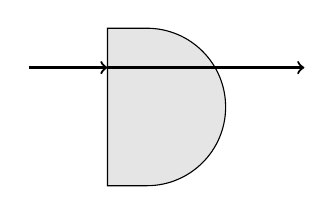
\begin{tikzpicture}
                %% semicircle
                \draw[fill=white!90!black] (-0.5,1) -- (0,1) arc (90:-90:1) -- (-0.5,-1) -- cycle;
                %% light ray
                \draw[thick,->] (-1.5,0.5) -- (-0.5,0.5);
                \draw[thick,->] (-0.5,0.5) -- (2,0.5);
            \end{tikzpicture}
        }
    \end{choices}
    \end{multicols}
\end{question}
}

\element{cap}{ %% cap-C1
\begin{question}{CAP-A-2013-q13}
    You put two identical ice cubes on plates of different materials. 
    One cube is put on an aluminum plate,
        and the other on a glass plate. 
    Both plates have been in the room for a long time prior to the experiment. 
    You notice that the ice melts faster on the metal plate. 
    Why?
    \begin{choices}
        \wrongchoice{The ice is in thermal equilibrium with the plastic plate, but not with the metal plate.}
      \correctchoice{The metal plate conducts heat to the ice more rapidly than the plastic plate.}
        \wrongchoice{The metal plate holds more heat than the plastic plate.}
        \wrongchoice{The metal plate was warmer than the plastic plate initially.}
    \end{choices}
\end{question}
}

\element{cap}{ %% cap-??
\begin{question}{CAP-A-2013-q14}
    Two black objects of the same diameter, a sphere and a flat disk,
        are placed in a parallel beam of light.  
    The plane of the disk is perpendicular to the beam.  
    What can be said about the force acting on them?
    \begin{choices}
        \wrongchoice{The force is zero.}
        \wrongchoice{The force is larger on the disk than on the sphere.}
        \wrongchoice{The force is larger on the sphere than on the disk.}
      \correctchoice{The force is the same on both objects.}
    \end{choices}
\end{question}
}

\element{cap}{ %% cap-B1
\begin{question}{CAP-A-2013-q15}
    Adrianne has a device that emits photons with a wavelength of $\lambda=\SI{1.498}{\kilo\meter}$.
    Kwan has a similar device that emits photons at a frequency of $f=\SI{201}{\kilo\hertz}$.
    Whose device emits photons in air at the highest frequency?
    \begin{choices}
        \wrongchoice{Adrianne's}
      \correctchoice{Kwan's}
        \wrongchoice{The frequencies are the same.}
        \wrongchoice{There is not enough information to compare.}
    \end{choices}
\end{question}
}

\element{cap}{ %% cap-??
\begin{question}{CAP-A-2013-q16}
    A girl sitting on a floating mattress in a small pool holds a model of a motorboat in her hands. 
    When she puts it in the water to start driving it with her remote control,
        what happens to the water level in the pool?
    \begin{choices}
        \wrongchoice{It rises by a small amount.}
        \wrongchoice{It drops by a small amount.}
      \correctchoice{It stays the same.}
        \wrongchoice{The qualitative result depends on the weight of the model boat.}
    \end{choices}
\end{question}
}

\element{cap}{ %% cap-XX-C3
\begin{question}{CAP-A-2013-q17}
    Which of the accompanying $P$--$V$ diagrams best represents an isothermal process,
        that is a process occurring at constant temperature?
    \begin{multicols}{2}
    \begin{choices}
        %% NOTE: ANS is B
        \AMCboxDimensions{down=-2.5em}
        \wrongchoice{
            \begin{tikzpicture}
                \begin{axis}[
                    axis y line=left, 
                    axis x line=bottom, 
                    axis line style={->},
                    xlabel={volume},
                    xtick=\empty,
                    ylabel={pressure},
                    ytick=\empty,
                    xmin=0,xmax=11,
                    ymin=0,ymax=11,
                    width=1.0\columnwidth,
                ]
                \addplot[line width=1pt,domain=0:10] { 8 };
                \end{axis}
            \end{tikzpicture}
        }
    \end{choices}
    \end{multicols}
\end{question}
}

\element{cap}{ %% cap-A3
\begin{question}{CAP-A-2013-q18}
    Two identical objects of mass $m$ are connected to a massless string which is hung over two frictionless pulleys as shown below. 
    %% NOTE: duplicate of olympiad-1995-q06
    \begin{center}
    \begin{tikzpicture}
        %% Ceiling
        \node[anchor=south,fill,pattern=north east lines,minimum width=8cm, minimum height=0.05cm] at (0,0) {};
        \draw (-4,0) -- (4,0);
        %% Mass Left
        \node[draw,anchor=north,minimum size=1cm,fill=white!90!black,rounded corners=0.5ex] (A) at (-2.5,-2.5) {$m$};
        %% Mass Right
        \node[draw,anchor=north,minimum size=1cm,fill=white!90!black,rounded corners=0.5ex] (B) at (+2.5,-2.5) {$m$};
        %% Rope
        \draw[very thick] (A.north) -- (-2.5,-1) arc(180:90:0.5) -- (+2,-0.5) arc(90:0:0.5) -- (B.north);
        %% Pulley Left
        \draw (-2,-1) circle (0.5cm);
        \draw[fill=white!90!black] (-2.2,0) -- (-2.1,-1.1) arc(190:350:0.1) -- (-1.8,0) -- cycle;
        \draw[fill] (-2,-1) circle (1pt);
        %% Pulley Right
        \draw (+2,-1) circle (0.5cm);
        \draw[fill=white!90!black] (+1.8,0) -- (+1.9,-1.1) arc(190:350:0.1) -- (+2.2,0) -- cycle;
        \draw[fill] (+2,-1) circle (1pt);
    \end{tikzpicture}
    \end{center}
    If everything is at rest,
        what is the tension in the cord?
    \begin{choices}
        \wrongchoice{Less than $mg$.}
      \correctchoice{Exactly $mg$.}
        \wrongchoice{More than $mg$, but less than $2mg$.}
        \wrongchoice{Exactly $2mg$.}
        \wrongchoice{More than $2mg$.}
    \end{choices}
\end{question}
}

\element{cap}{ %% cap-A1
\begin{question}{CAP-A-2013-q19}
    Car $A$ and car $B$ are both traveling down a straight highway at \SI{90}{\kilo\meter\per\hour}.
    Car $A$ is only \SI{6.0}{\meter} behind car $B$.
    The driver of car $B$ brakes,
        slowing down with a constant deceleration of \SI{2.0}{\meter\per\second\squared}.
    After \SI{1.2}{\second},
        the driver of car $A$ begins to brake,
        also at \SI{2.0}{\meter\per\second\squared},
        but this is insufficient and the cars eventually collide,
        both still moving forward. 
    What is the relative velocity of the two cars at the moment of the collision?
    \begin{multicols}{3}
    \begin{choices}
      \correctchoice{\SI{2.4}{\meter\per\second}}
        \wrongchoice{\SI{5.0}{\meter\per\second}}
        \wrongchoice{\SI{9.5}{\meter\per\second}}
        \wrongchoice{\SI{21}{\meter\per\second}}
        \wrongchoice{\SI{24}{\meter\per\second}}
    \end{choices}
    \end{multicols}
\end{question}
}

\element{cap}{ %% cap-B1
\begin{question}{CAP-A-2013-q20}
    Two interfering waves have the same wavelength, frequency, and amplitude. 
    They are traveling in the same direction but are 90 degrees out of phase. 
    Compared to the individual waves,
        what can be said about the resultant wave?
    \begin{choices}
        \wrongchoice{It will have the same amplitude and velocity, but a different wavelength.}
        \wrongchoice{It will have the same amplitude and wavelength, but a different velocity.}
      \correctchoice{It will have the same wavelength and velocity, but a different amplitude.}
        \wrongchoice{It will have the same amplitude and frequency, but a different velocity.}
        \wrongchoice{It will have the same frequency and velocity, but a different wavelength.}
    \end{choices}
\end{question}
}

\element{cap}{ %% cap-A6
\begin{question}{CAP-A-2013-q21}
    A spinning ice skater has an initial kinetic energy $\frac{1}{2} I\omega^2$.
    She pulls in her outstretched arms,
        decreasing her moment of inertia to $\frac{1}{4} I$.
    What is her new angular speed?
    \begin{multicols}{3}
    \begin{choices}
        \wrongchoice{$\dfrac{\omega}{4}$}
        \wrongchoice{$\dfrac{\omega}{2}$}
        \wrongchoice{$\omega$}
        \wrongchoice{$2\omega$}
      \correctchoice{$4\omega$}
    \end{choices}
    \end{multicols}
\end{question}
}

\element{cap}{ %% cap-A3
\begin{question}{CAP-A-2013-q22}
    A ball of mass $m$ is thrown vertically upward. 
    Instead of neglecting air resistance,
        assume that the force of air resistance has a magnitude proportional to the ball's velocity,
        but pointing in the opposite direction. 
    What is the ball's acceleration at the highest point?
    \begin{choices}
        \wrongchoice{zero}
        \wrongchoice{Less than $g$.}
      \correctchoice{$g$}
        \wrongchoice{Greater than $g$.}
    \end{choices}
\end{question}
}

\element{cap}{ %% cap-A7
\begin{question}{CAP-A-2013-q23}
    A hypothetical planet has density $\rho$, radius $R$,
        and surface gravitational acceleration $g$. 
    What would be the acceleration due to gravity at the surface of a planet with double the radius,
        and the same planetary density?
    \begin{multicols}{3}
    \begin{choices}
        \wrongchoice{$4g$}
      \correctchoice{$2g$}
        \wrongchoice{$g$}
        \wrongchoice{$\dfrac{g}{2}$}
        \wrongchoice{$\dfrac{g}{4}$}
    \end{choices}
    \end{multicols}
\end{question}
}

\element{cap}{ %% cap-B2
\begin{question}{CAP-A-2013-q24}
    You are given two lenses placed close together: a converging lens with focal length \SI{+10}{\centi\meter},
        and a diverging lens with focal length \SI{-20}{\centi\meter}.
    Which of the following would produce a virtual image that is larger than the object?
    \begin{choices}
      \correctchoice{Placing the object \SI{5}{\centi\meter} from the converging lens.}
        \wrongchoice{Placing the object \SI{15}{\centi\meter} from the converging lens.}
        \wrongchoice{Placing the object \SI{25}{\centi\meter} from the converging lens.}
        \wrongchoice{Placing the object \SI{15}{\centi\meter} from the diverging lens.}
        \wrongchoice{Placing the object \SI{25}{\centi\meter} from the diverging lens.}
    \end{choices}
\end{question}
}

\element{cap}{ %% cap-D5
\begin{question}{CAP-A-2013-q25}
    An electromagnetic wave is propagating in vacuum in the positive $z$ direction. 
    At an instant when its magnetic field $B$ at a certain position is in the positive $x$ direction and getting stronger,
        what happens to its electric field $E$ at that same position?
    \begin{choices}
        \wrongchoice{$E$ is in the positive $x$ direction and getting weaker.}
        \wrongchoice{$E$ is in the negative $x$ direction and getting stronger.}
        \wrongchoice{$E$ is in the positive $y$ direction and getting weaker.}
      \correctchoice{$E$ is in the negative $y$ direction and getting stronger.}
        \wrongchoice{$E$ is zero.}
    \end{choices}
\end{question}
}


%% CAP Exam 2012 Part A: Multiple Choice Questions
%%--------------------------------------------------
\element{cap}{ %% cap-XX-A7
\begin{question}{CAP-A-2012-q01}
    Two planets $X$ and $Y$ travel counterclockwise in circular orbits around a star as shown in the figure below:
    \begin{center}
    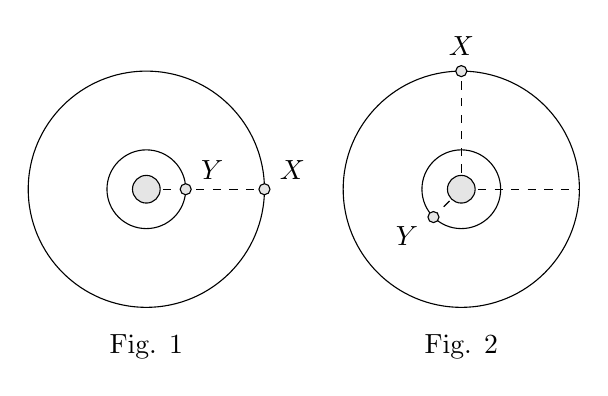
\begin{tikzpicture}
        \begin{scope}[xshift=-2cm]
            %% orbits
            \draw (0,0) circle (1.5cm);
            \draw (0,0) circle (0.5cm);
            %% Y and X
            \draw[dashed] (0,0) -- (1.5,0);
            \draw[fill=white!90!black] (0.5,0) circle (2pt) node[anchor=south west,xshift=2pt] {$Y$};
            \draw[fill=white!90!black] (1.5,0) circle (2pt) node[anchor=south west,xshift=2pt] {$X$};
            %% planet
            \draw[fill=white!90!black] (0,0)  circle (5pt);
            %% label
            \node[anchor=center] at (0,-2) {Fig. 1};
        \end{scope}
        \begin{scope}[xshift=+2cm]
            %% orbits
            \draw (0,0) circle (1.5cm);
            \draw (0,0) circle (0.5cm);
            %% Y and X
            \draw[dashed] (0,0) -- (1.5,0);
            \draw[dashed] (0,0) -- ++(90:1.5);
            \draw[dashed] (0,0) -- ++(225:0.5);
            \draw[fill=white!90!black] (225:0.5) circle (2pt) node[anchor=north east,xshift=-2pt] {$Y$};
            \draw[fill=white!90!black] (90:1.5) circle (2pt) node[anchor=south,yshift=2pt] {$X$};
            %% planet
            \draw[fill=white!90!black] (0,0)  circle (5pt);
            %% label
            \node[anchor=center] at (0,-2) {Fig. 2};
        \end{scope}
    \end{tikzpicture}
    \end{center}
    The radii of their orbits are in the ratio $3:1$. 
    At some time, they are aligned as in Fig. 1, making a straight line with the star. 
    After five Earth years, the angular displacement of planet $X$ is \ang{90.0},
        as in Fig. 2. 
    %% NOTE: angular displacement or angular distance??
    What is the angular displacement of planet $Y$ at this time?
    \begin{multicols}{3}
    \begin{choices}
        \wrongchoice{\ang{35}}
        \wrongchoice{\ang{90}}
        \wrongchoice{\ang{180}}
        \wrongchoice{\ang{360}}
      \correctchoice{\ang{468}}
    \end{choices}
    \end{multicols}
\end{question}
}

\element{cap}{ %% cap-A3
\begin{question}{CAP-A-2012-q02}
    You are holding a bottle of sparkling water inside a car moving forward. 
    When the driver applies the brakes:
    \begin{choices}
        \wrongchoice{Bubbles in the middle of the liquid will start to move forward with respect to the bottle.}
      \correctchoice{Bubbles will start to move backward with respect the bottle.}
        \wrongchoice{Bubbles will stay at the same horizontal location in the water.}
        \wrongchoice{Depending on the speed of the car, bubbles might move forward or backward.}
    \end{choices}
\end{question}
}

\element{cap}{ %% cap-A7
\begin{question}{CAP-A-2012-q03}
    An Earth satellite revolves in a circular orbit at a height $h$ from the surface of the Earth. 
    If $R$ is the Earth's radius and $g$ is the acceleration due to gravity at the surface of the Earth,
        then the speed of the satellite is given by:
    \begin{multicols}{2}
    \begin{choices}
        \wrongchoice{$\sqrt{gR}$}
        \wrongchoice{$\sqrt{g \left(R+h\right)}$}
      \correctchoice{$\sqrt{g \dfrac{R^2}{R+h}}$}
        \wrongchoice{$\sqrt{g \dfrac{\left(R+h\right)^2}{R}}$}
    \end{choices}
    \end{multicols}
\end{question}
}

\element{cap}{ %% cap-??
\begin{question}{CAP-A-2012-q04}
    Assume that sodium produces monochromatic light with a wavelength of \SI{5.89e-7}{\meter}.
    At what approximate rate would a 10 watt sodium-vapor light be emitting photons? 
    Assume that the efficiency of the light bulb is about \SI{30}{\percent}.
    \begin{multicols}{2}
    \begin{choices}
      \correctchoice{\SI{8.9e18}{photons\per\second}}
        \wrongchoice{\SI{3.0e19}{photons\per\second}}
        \wrongchoice{\SI{9.9e19}{photons\per\second}}
        \wrongchoice{\SI{2.0e20}{photons\per\second}}
    \end{choices}
    \end{multicols}
\end{question}
}

\element{cap}{ %% cap-D2
\begin{question}{CAP-A-2012-q05}
    Three batteries are placed in series. 
    Each battery has an internal resistance $r$. 
    If one of the batteries is placed the wrong way around as shown in the picture,
    \begin{center}
    \ctikzset{bipoles/length=1.00cm}
    \begin{circuitikz}[scale=1.1]
        %% nodes A and B
        \draw[fill] (-3,0) circle (2pt);
        \draw[fill] (+3,0) circle (2pt);
        %% Circuit
        \draw (-1,0) to [battery,v=$ $] (-3,0);
        \draw (-1,0) to [battery,v=$ $] (1,0) to [battery,v=$ $] (3,0);
    \end{circuitikz}
    \end{center}
        what will be the total resistance of the three cells now?
    \begin{multicols}{3}
    \begin{choices}
        \wrongchoice{$\dfrac{r}{3}$}
        \wrongchoice{$\dfrac{r}{2}$}
        \wrongchoice{$r$}
        \wrongchoice{$2r$}
      \correctchoice{$3r$}
    \end{choices}
    \end{multicols}
\end{question}
}

\element{cap}{ %% cap-??
\begin{question}{CAP-A-2012-q06}
    At the designed intensity, the two beams circulating in the Large Hadron Collider (LHC) at CERN consist of 5616 bunches (2808 in each direction) of approximately \num{1.15e11} protons per bunch. 
    A small commercial hydrogen cylinder contains \SI{40}{\liter} of gas at a pressure of \SI{10}{\mega\pascal} and a temperature of \SI{25}{\degreeCelsius}. 
    Assuming an injection efficiency of \SI{70}{\percent},
        how many times could the LHC be filled at the designed intensity using a single,
        perfectly hermetic cylinder?
    \begin{multicols}{2}
    \begin{choices}
        \wrongchoice{\num{1.1e11}}
        \wrongchoice{\num{1.5e11}}
      \correctchoice{\num{2.1e11}}
        \wrongchoice{\num{1.1e14}}
        \wrongchoice{\num{1.5e14}}
    \end{choices}
    \end{multicols}
\end{question}
}

\element{cap}{ %% cap-C1
\begin{question}{CAP-A-2012-q07}
    The Earth is constantly receiving energy from the Sun.
    To stay at approximately the same temperature,
        the Earth loses energy by:
    \begin{choices}
        \wrongchoice{Conduction}
      \correctchoice{Radiation}
        \wrongchoice{Convection}
        \wrongchoice{Evaporation}
        \wrongchoice{The Earth does not lose energy, this is why we have global warming.}
    \end{choices}
\end{question}
}

\element{cap}{ %% cap-A4
\begin{question}{CAP-A-2012-q08}
    A car starts to move at time $t=0$. 
    If the engine of the car is able to provide constant power,
        which of the following statements is correct about the speed of car at the beginning of the motion?
    \begin{choices}
        \wrongchoice{The speed is constant.}
        \wrongchoice{The speed increases proportionally to time passed ($v \propto t$).}
      \correctchoice{The speed increases as the square root of time ($v \propto \sqrt{t}$).}
        \wrongchoice{The speed increases as time squared ($v \propto t^2$).}
    \end{choices}
\end{question}
}

\element{cap}{ %% cap-A1
\begin{question}{CAP-A-2012-q09}
    A detector far away from the source of a wave is detecting pulses of that wave every 0.2 second. 
    If the detector starts to move towards the source at a speed of \SI{6.0}{\kilo\meter\per\hour},
        then it would detect a total of 18200 pulses per hour. 
    What is the speed of the wave?
    \begin{multicols}{2}
    \begin{choices}
        \wrongchoice{\SI{100}{\meter\per\second}}
      \correctchoice{\SI{150}{\meter\per\second}}
        \wrongchoice{\SI{200}{\meter\per\second}}
        \wrongchoice{\SI{300}{\meter\per\second}}
    \end{choices}
    \end{multicols}
\end{question}
}

\element{cap}{ %% cap-??
\begin{question}{CAP-A-2012-q10}
    There are three different liquids, with densities $\rho_1$, $\rho_2$ and $\rho_3$,
        in a U-shaped container as shown in the picture. 
        The lengths shown are $H_1=\SI{15}{\centi\meter}$ and $H_2=\SI{10}{\centi\meter}$.
    \begin{center}
    \begin{tikzpicture}[xscale=1.2]
        %% bottom rho_2
        \draw[fill=white!60!black] (-1.25,2) -- (-1.25,0) -- (1.25,0) -- (1.25,2.66) -- (1,2.66) -- (1,0.25) -- (-1,0.25) -- (-1,2) --cycle;
        \node[anchor=south] at (0,0.25) {$\rho_2$};
        %% left rho_3
        \draw[fill=white!90!black] (-1.25,2) rectangle (-1,4);
        \draw[<->] (-0.5,2) -- (-0.5,4)  node[pos=0.5,anchor=center,fill=white] {$H_1$};
        \node[anchor=east] at (-1.25,3) {$\rho_3$};
        %% right rho_1
        \draw[] (1,2.66) rectangle (1.25,4);
        \node[anchor=south,fill,pattern=north west lines,minimum width=0.2cm, minimum height=1.33cm] at (1.13,2.66) {};
        \draw[<->] (0.5,2.66) -- (0.5,4)  node[pos=0.5,anchor=center,fill=white] {$H_2$};
        \node[anchor=west] at (+1.25,3.33) {$\rho_1$};
        %% dashed line
        \draw[dashed] (-1,4) -- (1,4);
        \draw (-1.25,2) -- (-1.25,5);
        \draw (-1,2) -- (-1,5);
        \draw (+1.25,2) -- (+1.25,5);
        \draw (+1,2) -- (+1,5);
    \end{tikzpicture}
    \end{center}
    Which of the following equations gives the correct relation between the densities of the fluids in the container?
    \begin{multicols}{2}
    \begin{choices}
      \correctchoice{$3\rho_3   = 2\rho_1 +  \rho_2$}
        \wrongchoice{$ \rho_3   = 2\rho_1 + 3\rho_2$}
        \wrongchoice{$2\rho_3   = 3\rho_1 +  \rho_2$}
        \wrongchoice{$ \rho_3   = 3\rho_1 + 2\rho_2$}
    \end{choices}
    \end{multicols}
\end{question}
}

\element{cap}{ %% cap-??
\begin{question}{CAP-A-2012-q11}
    The intensity of light from a source decreases with the distance $x$ from the source, as $x^{-2}$.
    In the following picture, the intensity of light from the source $S$ at point $A$ on a curtain is \SI{8.1}{U} where U is some unit. 
    We then add a big mirror parallel to the curtain at point $B$.
    The distances $AS$ and $SB$ are equal,
        and the points $A$, $S$ and $B$ are in line perpendicular to the curtain and the mirror.
    \begin{center}
    \begin{tikzpicture}
        %% left and right
        \draw[dashed] (-3,-2) -- (-3,2);
        \draw[thick] (3,-2) -- (3,2);
        %% source
        \draw[fill] (0,0) circle (3pt) node[anchor=north,yshift=-5pt] {$S$};
        %% Rays
        \foreach \x in {60,120,...,360} \draw[thick,->] (0,0) -- (\x:1);
        %% A and B
        \draw[fill] (+3,0) circle (1.5pt) node[anchor=west,xshift=+1pt] {$A$};
        \draw[fill] (-3,0) circle (1.5pt) node[anchor=west,xshift=+1pt] {$B$};
        %% L and L
        \draw[<->] (-3,-1.5) -- (-0.05,-1.5) node[pos=0.5,anchor=center,fill=white] {$L$}; 
        \draw[<->] (+3,-1.5) -- (+0.05,-1.5) node[pos=0.5,anchor=center,fill=white] {$L$}; 
    \end{tikzpicture}
    \end{center}
    What is the intensity of light reaching point $A$ now?
    \begin{multicols}{2}
    \begin{choices}
      \correctchoice{\SI{9.0}{U}}
        \wrongchoice{\SI{10.15}{U}}
        \wrongchoice{\SI{10.8}{U}}
        \wrongchoice{\SI{16.2}{U}}
    \end{choices}
    \end{multicols}
\end{question}
}

\element{cap}{ %% cap-??
\begin{question}{CAP-A-2012-q12}
    Which of the following is the correct free-body diagram for a cylinder floating in water?
    \begin{multicols}{2}
    \begin{choices}
        \AMCboxDimensions{down=-2.5cm}
        \wrongchoice{
            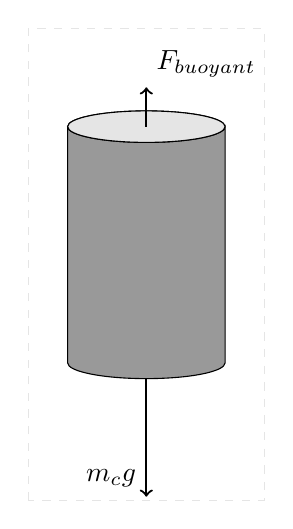
\begin{tikzpicture}
                \draw[dashed,white!90!black] (-1.5,-4.75) rectangle (1.5,1.25);
                %% cylinder
                \draw[fill=white!60!black] (-1,0) -- (-1,-3) arc (180:360:1cm and 0.2cm) -- (1,0) arc(360:-180:1cm and 0.2cm);
                \draw[fill=white!90!black] (0,0) circle (1cm and 0.2cm);
                %% Forces
                \draw[thick,->] (0,0) -- ++(90:0.5) node[anchor=south west] {$F_{\text{buoyant}}$};
                \draw[thick,->] (0,-3.2) -- ++(270:1.5) node[anchor=south east] {$m_c g$};
            \end{tikzpicture}
        }
        \wrongchoice{
            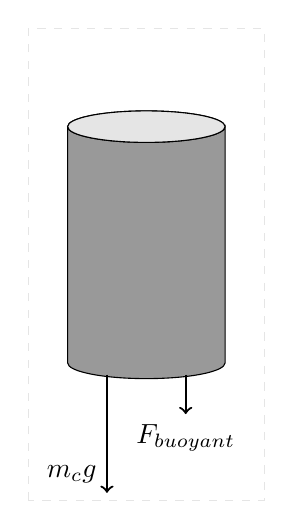
\begin{tikzpicture}
                \draw[dashed,white!90!black] (-1.5,-4.75) rectangle (1.5,1.25);
                %% cylinder
                \draw[fill=white!60!black] (-1,0) -- (-1,-3) arc (180:360:1cm and 0.2cm) -- (1,0) arc(360:-180:1cm and 0.2cm);
                \draw[fill=white!90!black] (0,0) circle (1cm and 0.2cm);
                %% Forces
                \draw[thick,->] (-0.5,-3.15) -- ++(270:1.50) node[anchor=south east] {$m_c g$};
                \draw[thick,->] (+0.5,-3.15) -- ++(270:0.50) node[anchor=north] {$F_{\text{buoyant}}$};
            \end{tikzpicture}
        }
        \wrongchoice{
            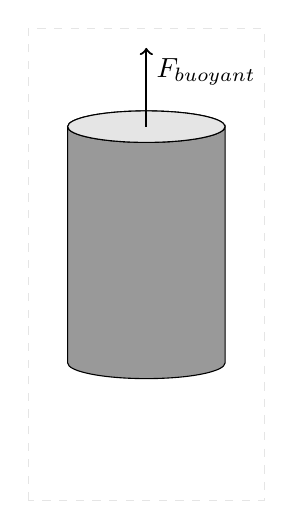
\begin{tikzpicture}
                \draw[dashed,white!90!black] (-1.5,-4.75) rectangle (1.5,1.25);
                %% cylinder
                \draw[fill=white!60!black] (-1,0) -- (-1,-3) arc (180:360:1cm and 0.2cm) -- (1,0) arc(360:-180:1cm and 0.2cm);
                \draw[fill=white!90!black] (0,0) circle (1cm and 0.2cm);
                %% Forces
                \draw[thick,->] (0,0) -- ++(90:1) node[anchor=north west] {$F_{\text{buoyant}}$};
            \end{tikzpicture}
        }
        %% ANS is D
        \correctchoice{
            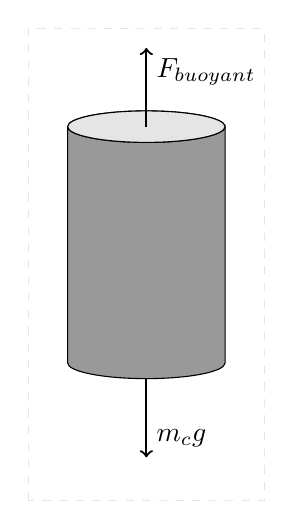
\begin{tikzpicture}
                \draw[dashed,white!90!black] (-1.5,-4.75) rectangle (1.5,1.25);
                %% cylinder
                \draw[fill=white!60!black] (-1,0) -- (-1,-3) arc (180:360:1cm and 0.2cm) -- (1,0) arc(360:-180:1cm and 0.2cm);
                \draw[fill=white!90!black] (0,0) circle (1cm and 0.2cm);
                %% Forces
                \draw[thick,->] (0,0) -- ++(90:1) node[anchor=north west] {$F_{\text{buoyant}}$};
                \draw[thick,->] (0,-3.2) -- ++(270:1) node[anchor=south west] {$m_c g$};
            \end{tikzpicture}
        }
    \end{choices}
    \end{multicols}
\end{question}
}

\element{cap}{ %% cap-??-M1
\begin{question}{CAP-A-2012-q13}
    Vancouver's latitude is about \ang{49},
        and Earth's axial tilt is about \ang{23}.
    The power delivered by the Sun reaching a horizontal surface in Vancouver at noon differs in winter and summer. 
    What is the approximate ratio of this quantity measured in winter,
        compared to that measured in summer?
    \begin{multicols}{2}
    \begin{choices}
        \wrongchoice{$1:2$}
      \correctchoice{$1:3$}
        \wrongchoice{$1:4$}
        \wrongchoice{$1:5$}
    \end{choices}
    \end{multicols}
\end{question}
}

\element{cap}{ %% cap-B1
\begin{question}{CAP-A-2012-q14}
    Consider a metal rod firmly attached to a wall. 
    \begin{center}
    \begin{tikzpicture}
        %% wall
        \draw (0,-1) -- (0,1);
        \node[anchor=west,fill,pattern=north east lines,minimum width=0.05cm, minimum height=2cm] at (0,0) {};
        %% rod
        \draw[fill=white!90!black] (0,-1ex) rectangle (-5,1ex);
        %% hammer
        \begin{scope}[rotate=-45,xshift=-4.5cm,yshift=-5cm]
            %% handle
            \draw[fill=white!90!black] (-1ex,0) -- (-0.5ex,2) -- (0.5ex,2) -- (1ex,0) -- cycle;
            %% mallet
            \draw[fill=white!60!black] (-2ex,2) -- (-1.5ex,2.2) -- (1.5ex,2.2) -- (2ex,2) -- cycle;
            \draw[fill] (-4ex,2.2) -- (-4ex,2.7) -- (4ex,2.7) -- (4ex,2.2) -- cycle;
        \end{scope}
    \end{tikzpicture}
    \end{center}
    When you strike the rod with a hammer,
        which kind of wave Which of the following is the closest to the total mass will you excite?
    \begin{choices}
        \wrongchoice{A longitudinal wave.}
        \wrongchoice{A transverse wave.}
      \correctchoice{Either kind, or both, depending on where and how you hit the rod.}
        \wrongchoice{No wave will be excited, the metal is too strong.}
    \end{choices}
\end{question}
}

\element{cap}{ %% cap-A1
\begin{question}{CAP-A-2012-q15}
    Assume that you videotaped the fall of a ball due to gravity in vacuum,
        and are now playing the video in reverse at the same speed. 
    Which of the following statements is correct about the acceleration of the ball seen in these conditions,
        compared to that of the actual falling ball?
    \begin{choices}
      \correctchoice{The accelerations are the same in both cases.}
        \wrongchoice{They have the same value but opposite directions.}
        \wrongchoice{They have different values but the same direction.}
        \wrongchoice{Both the values and directions differ.}
    \end{choices}
\end{question}
}

\element{cap}{ %% cap-A6
\begin{question}{CAP-A-2012-q16}
    A rod ($AB$) is attached to a fixed point ($C$) using a light rope ($AC$). 
    The other end of the rod ($B$) is sitting on ice with negligible friction and the system is in stationary position. 
    Which of the following can be the equilibrium configuration of this system?
    \begin{multicols}{2}
    \begin{choices}
        \AMCboxDimensions{down=-1cm}
        \wrongchoice{
            \begin{tikzpicture}
                %% floor
                \draw (0,0) -- (3,0);
                \node[anchor=north,fill,pattern=north east lines,minimum width=3cm, minimum height=0.05cm] at (1.5,0) {};
                %% coordinate A, B, C
                \coordinate (A) at (0.5,2);
                \coordinate (B) at (+2,0);
                \coordinate (C) at (+2,2);
                %% lables
                \draw[fill] (A) circle (1.5pt) node[anchor=east] {$A$};
                \draw[fill] (B) circle (1.5pt) node[anchor=south west] {$B$};
                \draw[fill] (C) circle (1.5pt) node[anchor=west] {$C$};
                %% Rod AB, rope AC
                \draw[very thick] (A) -- (B);
                \draw[thin] (A) -- (C);
                \draw[dashed] (C) -- (B);
            \end{tikzpicture}
        }
        \wrongchoice{
            \begin{tikzpicture}
                %% floor
                \draw (0,0) -- (3,0);
                \node[anchor=north,fill,pattern=north east lines,minimum width=3cm, minimum height=0.05cm] at (1.5,0) {};
                %% coordinate A, B, C
                \coordinate (A) at (0.5,1.5);
                \coordinate (B) at (+2.5,0);
                \coordinate (C) at (1.5,2);
                %% lables
                \draw[fill] (A) circle (1.5pt) node[anchor=east] {$A$};
                \draw[fill] (B) circle (1.5pt) node[anchor=south west] {$B$};
                \draw[fill] (C) circle (1.5pt) node[anchor=west] {$C$};
                %% Rod AB, rope AC
                \draw[dashed] (C) -- (1.5,0);
                \draw[very thick] (A) -- (B);
                \draw[thin] (A) -- (C);
            \end{tikzpicture}
        }
        %% ANS: is C
        \correctchoice{
            \begin{tikzpicture}
                %% floor
                \draw (0,0) -- (3,0);
                \node[anchor=north,fill,pattern=north east lines,minimum width=3cm, minimum height=0.05cm] at (1.5,0) {};
                %% coordinate A, B, C
                \coordinate (A) at (0.5,1.25);
                \coordinate (B) at (+2.75,0);
                \coordinate (C) at (0.5,2);
                %% lables
                \draw[fill] (A) circle (1.5pt) node[anchor=east] {$A$};
                \draw[fill] (B) circle (1.5pt) node[anchor=south] {$B$};
                \draw[fill] (C) circle (1.5pt) node[anchor=west] {$C$};
                %% Rod AB, rope AC
                \draw[dashed] (C) -- (0.5,0);
                \draw[very thick] (A) -- (B);
                \draw[thin] (A) -- (C);
            \end{tikzpicture}
        }
        \wrongchoice{
            \begin{tikzpicture}
                %% floor
                \draw (0,0) -- (3,0);
                \node[anchor=north,fill,pattern=north east lines,minimum width=3cm, minimum height=0.05cm] at (1.5,0) {};
                %% coordinate A, B, C
                \coordinate (A) at (1,1);
                \coordinate (B) at (+2.75,0);
                \coordinate (C) at (0.25,2);
                %% lables
                \draw[fill] (A) circle (1.5pt) node[anchor=south west] {$A$};
                \draw[fill] (B) circle (1.5pt) node[anchor=south] {$B$};
                \draw[fill] (C) circle (1.5pt) node[anchor=west] {$C$};
                %% Rod AB, rope AC
                \draw[dashed] (C) -- (0.25,0);
                \draw[very thick] (A) -- (B);
                \draw[thin] (A) -- (C);
            \end{tikzpicture}
        }
    \end{choices}
    \end{multicols}
\end{question}
}

\element{cap}{ %% cap-??-M3
\begin{question}{CAP-A-2012-q17}
    Which of the following is the closest to the total mass of the atmosphere around the Earth?
    \begin{multicols}{2}
    \begin{choices}
        \wrongchoice{\SI{e13}{\kilo\gram}}
        \wrongchoice{\SI{e16}{\kilo\gram}}
      \correctchoice{\SI{e19}{\kilo\gram}}
        \wrongchoice{\SI{e22}{\kilo\gram}}
    \end{choices}
    \end{multicols}
\end{question}
}

\element{cap}{ %% cap-??
\begin{question}{CAP-A-2012-q18}
    At shallow depth, $h$, the pressure in the ocean is simply given by $P = P_0 + \rho gh$,
        in which $\rho$ is the density of water and $P_0$ is the air pressure. 
    As we go deeper,
        the high pressure causes the water to compress and become denser. 
    Which of the following sketches illustrates the correct dependence of the pressure on the depth $h$?
    \begin{multicols}{2}
    \begin{choices}
        \AMCboxDimensions{down=-2.5em}
        %% ANS is A
        \correctchoice{
            \begin{tikzpicture}
                \begin{axis}[
                    axis y line=left, 
                    axis x line=bottom, 
                    axis line style={->},
                    xlabel={$h$},
                    x label style={
                        at={(current axis.right of origin)},
                        anchor=north east,
                    },
                    xtick=\empty,
                    ylabel={$P$},
                    y label style={
                        at={(current axis.above origin)},
                        anchor=north east,
                        rotate=270,
                    },
                    ytick={2},
                    yticklabels={$P_0$},
                    xmin=0,xmax=11,
                    ymin=0,ymax=11,
                    width=1.0\columnwidth,
                ]
                \addplot[line width=1pt,domain=0:10] { 2 + 0.08 * x*x };
                \end{axis}
            \end{tikzpicture}
        }
        \wrongchoice{
            \begin{tikzpicture}
                \begin{axis}[
                    axis y line=left, 
                    axis x line=bottom, 
                    axis line style={->},
                    xlabel={$h$},
                    x label style={
                        at={(current axis.right of origin)},
                        anchor=north east,
                    },
                    xtick=\empty,
                    ylabel={$P$},
                    y label style={
                        at={(current axis.above origin)},
                        anchor=north east,
                        rotate=270,
                    },
                    ytick={2},
                    yticklabels={$P_0$},
                    xmin=0,xmax=11,
                    ymin=0,ymax=11,
                    width=1.0\columnwidth,
                ]
                \addplot[line width=1pt] plot coordinates { (0,2) (10,10) };
                \end{axis}
            \end{tikzpicture}
        }
        \wrongchoice{
            \begin{tikzpicture}
                \begin{axis}[
                    axis y line=left, 
                    axis x line=bottom, 
                    axis line style={->},
                    xlabel={$h$},
                    x label style={
                        at={(current axis.right of origin)},
                        anchor=north east,
                    },
                    xtick=\empty,
                    ylabel={$P$},
                    y label style={
                        at={(current axis.above origin)},
                        anchor=north east,
                        rotate=270,
                    },
                    ytick={2},
                    yticklabels={$P_0$},
                    xmin=0,xmax=11,
                    ymin=0,ymax=11,
                    width=1.0\columnwidth,
                ]
                \addplot[line width=1pt,domain=0:10] { -6 + 16 / (1 + exp(-0.5*x) ) };
                \draw[dashed] (axis cs:0,10) -- (axis cs:10,10);
                \end{axis}
            \end{tikzpicture}
        }
        \wrongchoice{
            \begin{tikzpicture}
                \begin{axis}[
                    axis y line=left, 
                    axis x line=bottom, 
                    axis line style={->},
                    xlabel={$h$},
                    x label style={
                        at={(current axis.right of origin)},
                        anchor=north east,
                    },
                    xtick=\empty,
                    ylabel={$P$},
                    y label style={
                        at={(current axis.above origin)},
                        anchor=north east,
                        rotate=270,
                    },
                    ytick={2},
                    yticklabels={$P_0$},
                    xmin=0,xmax=11,
                    ymin=0,ymax=11,
                    width=1.0\columnwidth,
                ]
                \addplot[line width=1pt,domain=0:10] { 2 + 2.52*sqrt(x) };
                \end{axis}
            \end{tikzpicture}
        }
    \end{choices}
    \end{multicols}
\end{question}
}

\element{cap}{ %% cap-C1
\begin{question}{CAP-A-2012-q19}
    An aluminum plate and a glass plate are left in a room for a long time. 
    Putting one ice cube on each plate,
        you notice that the ice melts faster on the aluminum plate. 
    Why?
    \begin{choices}
        \wrongchoice{The ice is in thermal equilibrium with the glass plate, but not with the aluminum plate.}
      \correctchoice{Aluminum conducts heat to the ice more rapidly than glass.}
        \wrongchoice{The aluminum plate holds more heat.}
        \wrongchoice{The aluminum plate is warmer.}
    \end{choices}
\end{question}
}

\element{cap}{ %% cap-B4
\begin{question}{CAP-A-2012-q20}
    You are on the side of the highway,
        listening to the siren of a fast-approaching ambulance. 
    When the ambulance is not moving the frequency of its siren is \SI{1000}{\hertz}.
    Which of the following graphs best describes the frequency that you hear as the ambulance approaches and then passes you?
    \begin{choices}
        %% NOTE: make graphs better??
        \AMCboxDimensions{down=-4em}
        \wrongchoice{
            \begin{tikzpicture}
                \begin{axis}[
                    axis y line=left, 
                    axis x line=bottom, 
                    axis line style={->},
                    xlabel={time},
                    x unit=\si{\second},
                    xtick={0,1,2,3,4,5,6},
                    ylabel={frequency},
                    y unit=\si{\hertz},
                    ytick={920,960,1000,1040,1080},
                    xmin=0,xmax=6.5,
                    ymin=920,ymax=1090,
                    width=0.8\columnwidth,
                    height=0.5\columnwidth,
                ]
                \addplot[line width=1pt] plot coordinates { (1,1080) (5,920) };
                \end{axis}
            \end{tikzpicture}
        }
        \wrongchoice{
            \begin{tikzpicture}
                \begin{axis}[
                    axis y line=left, 
                    axis x line=bottom, 
                    axis line style={->},
                    xlabel={time},
                    x unit=\si{\second},
                    xtick={0,1,2,3,4,5,6},
                    ylabel={frequency},
                    y unit=\si{\hertz},
                    ytick={920,960,1000,1040,1080},
                    xmin=0,xmax=6.5,
                    ymin=920,ymax=1090,
                    width=0.8\columnwidth,
                    height=0.5\columnwidth,
                ]
                \addplot[line width=1pt] plot coordinates { (1,920) (5,1080) };
                \end{axis}
            \end{tikzpicture}
        }
        %% ANS is C
        \correctchoice{
            \begin{tikzpicture}
                \begin{axis}[
                    axis y line=left, 
                    axis x line=bottom, 
                    axis line style={->},
                    xlabel={time},
                    x unit=\si{\second},
                    xtick={0,1,2,3,4,5,6},
                    ylabel={frequency},
                    y unit=\si{\hertz},
                    ytick={920,960,1000,1040,1080},
                    xmin=0,xmax=6.5,
                    ymin=920,ymax=1090,
                    width=0.8\columnwidth,
                    height=0.5\columnwidth,
                ]
                \addplot[line width=1pt,domain=0:6] { 940 + 120 / (1 + exp(10*(x-3)) };
                \end{axis}
            \end{tikzpicture}
        }
        \wrongchoice{
            \begin{tikzpicture}
                \begin{axis}[
                    axis y line=left, 
                    axis x line=bottom, 
                    axis line style={->},
                    xlabel={time},
                    x unit=\si{\second},
                    xtick={0,1,2,3,4,5,6},
                    ylabel={frequency},
                    y unit=\si{\hertz},
                    ytick={920,960,1000,1040,1080},
                    xmin=0,xmax=6.5,
                    ymin=920,ymax=1090,
                    width=0.8\columnwidth,
                    height=0.5\columnwidth,
                ]
                \draw (axis cs:0,1060) to[out=0,in=180] (axis cs:6,940);
                \end{axis}
            \end{tikzpicture}
        }
    \end{choices}
\end{question}
}

\element{cap}{ %% cap-B1
\begin{question}{CAP-A-2012-q21}
    Which of the following radiation types has the longest wavelength?
    \begin{choices}
      \correctchoice{Radio Waves}
        \wrongchoice{Visible light}
        \wrongchoice{X rays}
        \wrongchoice{Infrared light}
        \wrongchoice{All of the provided have the same wavelength.}
    \end{choices}
\end{question}
}

\element{cap}{ %% cap-XX-??
\begin{question}{CAP-A-2012-q22}
    A cup filled with water has a hole in the side,
        through which the liquid is flowing out. 
    If the cup is dropped from a height,
        what will happen to the water flowing from the cup?
    \begin{choices}
        %% NOTE: TODO: each option has an accompany diagram also
        \wrongchoice{It will keep coming out, flowing at the same rate as before.}
        \wrongchoice{It will keep coming out, but it will flow a bit slower than  before.}
        \wrongchoice{It will keep coming out, but start to flow upwards relative to the cup:}
        \wrongchoice{It will keep coming out, flowing horizontally with respect to the falling cup:}
      \correctchoice{It will stop flowing.}
    \end{choices}
\end{question}
}

\element{cap}{ %% cap-??
\begin{question}{CAP-A-2012-q23}
    Two cubes, with respective masses $M_1$ and $M_2$ and side lengths $L_1$ and $L_2$,
        are lying on a smooth table as shown.
    \begin{center}
    \begin{tikzpicture}
        %% ground
        \draw (-3,0) -- (3,0);
        \node[anchor=north,fill,pattern=north east lines,minimum width=6cm, minimum height=0.05cm] at (0,0) {};
        %% M_1
        \draw[fill=white!90!black] (-1.5,0) rectangle (1.5,3);
        \node[anchor=center] at (0,1.5) {$M_1$};
        \node[anchor=east] at (-1.5,1.5) {$L_1$};
        %% M_2
        \draw[fill=white!60!black] (-0.66,3) rectangle (0.66,4.33);
        \node[anchor=center] at (0,3.66) {$M_2$};
        \node[anchor=east] at (-1,3.66) {$L_2$};
    \end{tikzpicture}
    \end{center}
    What is the pressure exerted by the cubes on the table?
    \begin{choices}
        \wrongchoice{$\dfrac{M_1 g}{L_1^2} + \dfrac{M_2 g}{L_2^2}$}
      \correctchoice{$\dfrac{M_1 g}{L_1^2} + \dfrac{M_2 g}{L_1^2}$}
        \wrongchoice{$\dfrac{M_1 g}{L_2^2} + \dfrac{M_2 g}{L_2^2}$}
        \wrongchoice{None of the provided}
    \end{choices}
\end{question}
}

\element{cap}{ %% cap-??
\begin{question}{CAP-A-2012-q24}
    Consider an object that floats in water but sinks in oil. 
    When the object floats in water, half of it is submerged. 
    If we slowly pour oil on top of the water so it completely covers the object,
        the object:
    \begin{choices}
      \correctchoice{moves up}
        \wrongchoice{stays in the same place}
        \wrongchoice{moves down}
    \end{choices}
\end{question}
}

\element{cap}{ %% cap-??
\begin{question}{CAP-A-2012-q25}
    The pressure in a stream of water flowing out of a faucet is:
    \begin{choices}
        \wrongchoice{largest at the bottom}
        \wrongchoice{largest near the faucet}
      \correctchoice{the same everywhere in the stream}
    \end{choices}
\end{question}
}


%% CAP Exam 2011 Part A: Multiple Choice Questions
%%--------------------------------------------------
\element{cap}{ %% cap-??
\begin{question}{CAP-A-2011-q01}
    Incandescent light bulbs are notorious for being relatively inefficient in producing visible light. 
    The tungsten wire inside such a bulb is at a temperature of approximately \SI{3000}{\kelvin} and the emission spectrum is very similar to that of a blackbody. 
    The efficiency is so low because:
    \begin{choices}
        \wrongchoice{Most of the electrons are absorbed in the tungsten wire.}
        \wrongchoice{Most of the power is lost due to the resistance of the bulb.}
      \correctchoice{The electric power actually is efficiently transformed into radiation but at \SI{3000}{\kelvin}, most of it is infrared.}
        \wrongchoice{A blackbody absorbs more light than it emits, hence it appears black.}
    \end{choices}
\end{question}
}

\element{cap}{
\begin{question}{CAP-A-2011-q02}
    A solar panel installed on a spaceship has a maximum energy output of \SI{5}{\kilo\watt} near the Earth. 
    What is the maximum energy output of the solar panel when the spaceship is near Mars? 
    (The distance from the Earth to the Sun is 1 A.U. and from Mars to the Sun is 1.5 A.U.)
    \begin{multicols}{3}
    \begin{choices}
        \wrongchoice{\SI{3.3}{\kilo\watt}}
      \correctchoice{\SI{2.2}{\kilo\watt}}
        \wrongchoice{\SI{1.0}{\kilo\watt}}
        \wrongchoice{\SI{0.55}{\kilo\watt}}
        \wrongchoice{\SI{0.20}{\kilo\watt}}
    \end{choices}
    \end{multicols}
\end{question}
}

\element{cap}{
\begin{question}{CAP-A-2011-q03}
    A scientist measured a 1μA current in an area of a human brain. 
    Unlike current in metals which is carried by free electrons,
        the current in the brain is mainly carried by potassium ions. 
    Each potassium ion has one unit of charge $e$. 
    This current corresponds to the flow of how many potassium ions per second?
    \begin{multicols}{3}
    \begin{choices}
        \wrongchoice{\num{6e5}}
        \wrongchoice{\num{6e6}}
        \wrongchoice{\num{6e8}}
      \correctchoice{\num{6e12}}
        \wrongchoice{\num{6e18}}
    \end{choices}
    \end{multicols}
\end{question}
}

\element{cap}{ %% cap-XX-C1
\begin{question}{CAP-A-2011-q04}
    The gas supply to your physics professor's house suddenly stops due to a gas line failure. 
    It is winter and the temperature outside is \SI{-5}{\degreeCelsius} and constant. 
    Assuming all the doors and windows remain closed,
        which of these graphs best describes how the temperature in the house changes with time after the gas supply stops?
    \begin{multicols}{2}
    \begin{choices}
        %% NOTE: ANS is C
        %% NOTE: TODO: pgfplots
        \AMCboxDimensions{down=-2.5em}
        \wrongchoice{
            \begin{tikzpicture}
                \begin{axis}[
                    axis y line=left, 
                    axis x line=bottom, 
                    axis line style={->},
                    xlabel={time},
                    x unit=\si{\hour},
                    xtick={0,10,20,30},
                    ylabel={temperature},
                    y unit=\si{\degreeCelsius},
                    ytick={-10,0,10,20,30},
                    xmin=0,xmax=31,
                    ymin=-11,ymax=31,
                    width=1.0\columnwidth,
                ]
                \addplot[line width=1pt] plot coordinates { (0,9) (3,9) };
                \end{axis}
            \end{tikzpicture}
        }
        \wrongchoice{
            \begin{tikzpicture}
                \begin{axis}[
                    axis y line=left, 
                    axis x line=bottom, 
                    axis line style={->},
                    xlabel={time},
                    x unit=\si{\hour},
                    xtick={0,10,20,30},
                    ylabel={temperature},
                    y unit=\si{\degreeCelsius},
                    ytick={-10,0,10,20,30},
                    xmin=0,xmax=31,
                    ymin=-11,ymax=31,
                    width=1.0\columnwidth,
                ]
                \addplot[line width=1pt] plot coordinates { (0,22) (30,-5) };
                \end{axis}
            \end{tikzpicture}
        }
    \end{choices}
    \end{multicols}
\end{question}
}

\element{cap}{ %% cap-XX-B2
\begin{question}{CAP-A-2011-q05}
    The ray of light traveling in air hits the parallel glass plate as shown.
    \begin{center}
    \begin{tikzpicture}
        %% NOTE: TODO: tikz draw
        %% Incoming
        \draw[thick,->] (-3,0) -- (0,0);
        %% reflected
        \draw (0,0) -- ++(120:1) node[anchor=south] {1};
    \end{tikzpicture}
    \end{center}
    Which are the possible continuations of the light ray?
    \begin{multicols}{2}
    \begin{choices}
        \wrongchoice{4 only}
        \wrongchoice{both 2 and 4}
        \wrongchoice{both 3 and 6}
      \correctchoice{both 1 and 5}
    \end{choices}
    \end{multicols}
\end{question}
}

\element{cap}{ %% cap-??-M3
\begin{question}{CAP-A-2011-q06}
    Approximately, what fraction of the energy emitted by the Sun reaches to the Earth?
    \begin{multicols}{2}
    \begin{choices}
        \wrongchoice{\num{e-7}}
      \correctchoice{\num{e-10}}
        \wrongchoice{\num{e-13}}
        \wrongchoice{\num{e-16}}
    \end{choices}
    \end{multicols}
\end{question}
}

%\element{cap}{
%\begin{question}{CAP-A-2011-q07}
%    The resistance of the tungsten in a light bulb increases with temperature.
%    Which of the following graphs shows the current as a function of voltage for the light bulb?
%    \begin{multicols}{2}
%    \begin{choices}
%        \AMCboxDimensions{down=-2.5em}
%        %% ANS is A
%        %% NOTE: this question is confusing and too subtle
%        \correctchoice{
%            \begin{tikzpicture}
%                \begin{axis}[
%                    axis y line=left, 
%                    axis x line=bottom, 
%                    axis line style={->},
%                    xlabel={voltage},
%                    xtick=\empty,
%                    ylabel={current},
%                    ytick=\empty,
%                    xmin=0,xmax=11,
%                    ymin=0,ymax=11,
%                    width=1.0\columnwidth,
%                ]
%                \addplot[line width=1pt,domain=0:10] { 3.16*sqrt(x) };
%                \end{axis}
%            \end{tikzpicture}
%        }
%        \wrongchoice{
%            \begin{tikzpicture}
%                \begin{axis}[
%                    axis y line=left, 
%                    axis x line=bottom, 
%                    axis line style={->},
%                    xlabel={voltage},
%                    xtick=\empty,
%                    ylabel={current},
%                    ytick=\empty,
%                    xmin=0,xmax=11,
%                    ymin=0,ymax=11,
%                    width=1.0\columnwidth,
%                ]
%                \addplot[line width=1pt,domain=0:10] { 0.1*x*x };
%                \end{axis}
%            \end{tikzpicture}
%        }
%        \wrongchoice{
%            \begin{tikzpicture}
%                \begin{axis}[
%                    axis y line=left, 
%                    axis x line=bottom, 
%                    axis line style={->},
%                    xlabel={voltage},
%                    xtick=\empty,
%                    ylabel={current},
%                    ytick=\empty,
%                    xmin=0,xmax=11,
%                    ymin=0,ymax=11,
%                    width=1.0\columnwidth,
%                ]
%                \addplot[line width=1pt,domain=0:10] { 10 - 0.1*(x-10)*(x-10) };
%                \end{axis}
%            \end{tikzpicture}
%        }
%        \wrongchoice{
%            \begin{tikzpicture}
%                \begin{axis}[
%                    axis y line=left, 
%                    axis x line=bottom, 
%                    axis line style={->},
%                    xlabel={voltage},
%                    xtick=\empty,
%                    ylabel={current},
%                    ytick=\empty,
%                    xmin=0,xmax=11,
%                    ymin=0,ymax=11,
%                    width=1.0\columnwidth,
%                ]
%                \addplot[line width=1pt,domain=0:10] { x };
%                \end{axis}
%            \end{tikzpicture}
%        }
%        %% NOTE: too similar to B
%        %\wrongchoice{
%        %    \begin{tikzpicture}
%        %        \begin{axis}[
%        %            axis y line=left, 
%        %            axis x line=bottom, 
%        %            axis line style={->},
%        %            xlabel={voltage},
%        %            xtick=\empty,
%        %            ylabel={current},
%        %            ytick=\empty,
%        %            xmin=0,xmax=11,
%        %            ymin=0,ymax=11,
%        %            width=1.0\columnwidth,
%        %        ]
%        %        \addplot[line width=1pt,domain=0:10] { 0.1*x*x };
%        %        \end{axis}
%        %    \end{tikzpicture}
%        %}
%    \end{choices}
%    \end{multicols}
%\end{question}
%}

\element{cap}{ %% cap-E3
\begin{question}{CAP-A-2011-q08}
    A fast rocket travels directly upwards at 0.5c (half the speed of light). 
    There is an explosion directly below the rocket. 
    If astronauts manage to measure how fast the light produced by the explosion is moving relative to their spacecraft,
        they will find the light to be moving:
    \begin{choices}
        \wrongchoice{Upwards at speed $0.5 c$.}
      \correctchoice{Upwards at speed $c$.}
        \wrongchoice{Upwards at speed $1.5 c$.}
        \wrongchoice{Downwards at speed $0.5 c$.}
        \wrongchoice{Downwards at speed $c$.}
    \end{choices}
\end{question}
}

\element{cap}{ %% cap-XX-E3
\begin{question}{CAP-A-2011-q09}
    Two identical clocks are set to the same time as one passes the other at very high (relativistic) velocity as shown in the top figure. 
    \begin{center}
    \begin{tikzpicture}
        %% NOTE: TODO: draw tikz
    \end{tikzpicture}
    \end{center}
    Which of the other figures represents a possible observation of the clocks at some later time in the reference frame of the stationary clock?
    \begin{multicols}{2}
    \begin{choices}
        %% NOTE: ANS is C
        \wrongchoice{
            \begin{tikzpicture}
                %% NOTE: TODO: pgfplots
            \end{tikzpicture}
        }
    \end{choices}
    \end{multicols}
\end{question}
}

\element{cap}{ %% cap-E3
\begin{questionmult}{CAP-A-2011-q10}
    %For the statements:
    %\begin{enumerate}
    %    \item Mass can be directly converted into kinetic energy
    %    \item Kinetic energy can be directly converted into mass
    %\end{enumerate}
    Of the below statements, which are true?
    \begin{choices}
        \correctchoice{Mass can be directly converted into kinetic energy}
        \correctchoice{Kinetic energy can be directly converted into mass}
        %\wrongchoice{only first is true}
        %\wrongchoice{only second is true}
        %\correctchoice{both are true}
        %\wrongchoice{neither is true}
    \end{choices}
\end{questionmult}
}

\element{cap}{ %% cap-E2
\begin{question}{CAP-A-2011-q11}
    A stable Helium-4 nucleus has two protons and two neutrons.
    If the mass of Helium-4 nucleus,
        proton and neutron are denote by $m_{\ce{He}}$, $m_p$, $m_n$ respectively,
        we can conclude that:
    \begin{choices}
        \wrongchoice{$m_{\ce{He}} = 2m_p + 2m_a$}
        \wrongchoice{$m_{\ce{He}} > 2m_p + 2m_a$}
      \correctchoice{$m_{\ce{He}} < 2m_p + 2m_a$}
        \wrongchoice{Any of the provided may be true.}
    \end{choices}
\end{question}
}

\element{cap}{ %% cap-??
\begin{question}{CAP-A-2011-q12}
    A clean metal surface is placed in a vacuum.
    The surface is irradiated with monochromatic light of variable intensity $I$ (number of photons per unit area) and frequency $f$.
    We measure the maximum kinetic energy $K$ of electrons emitted from the meter due to the photoelectric effect.
    How does $K$ behave when $I$ increases?
    \begin{choices}
        \wrongchoice{$K$ increases}
      \correctchoice{$K$ is constant}
        \wrongchoice{$K$ decreases}
        \wrongchoice{Impossible to determine}
    \end{choices}
\end{question}
}

\element{cap}{ %% cap-A2
\begin{question}{CAP-A-2011-q13}
    A point mass is moving in the $xy$ plane.
    Its acceleration is a constant vector perpendicular to the $x$ axis,
        then:
    \begin{choices}
        \wrongchoice{only $v_y$ is constant.}
        \wrongchoice{only $v_x$ is constant.}
        \wrongchoice{only the acceleration is constant.}
      \correctchoice{the acceleration and $v_x$ are constant.}
        \wrongchoice{the position and $a_y$ are constant.}
    \end{choices}
\end{question}
}

\element{cap}{ %% cap-A3
\begin{question}{CAP-A-2011-q14}
    A huge case, attached to a cable,
        is descending at a constant velocity. 
    The tension in the cable is (neglecting the air resistance):
    \begin{choices}
        \wrongchoice{greater than the weight of the case.}
        \wrongchoice{smaller than the weight of the case.}
      \correctchoice{equal to the weight of the case.}
        \wrongchoice{we cannot tell since we don't know the weight of the case.}
    \end{choices}
\end{question}
}

\element{cap}{ %% cap-C1
\begin{question}{CAP-A-2011-q15}
    Objects $A$ and $B$, isolated from the environment,
        are initially separated from each other and are then placed in thermal contact. 
    Their initial temperatures are $T_A=\SI{0}{\degreeCelsius}$ and $T_B=\SI{100}{\degreeCelsius}$. 
    The heat capacity of $B$ is twice the one of $A$. 
    \begin{center}
    \begin{tikzpicture}
        %% Block A
        \draw (0,0) rectangle (2,2);
        %% label A
        \node[anchor=center] (A) at (1,1) {\SI{1.0}{\kilo\gram}};
        \node[anchor=south] at (A.north) {$A$};
        \node[anchor=north] at (A.south) {\SI{0}{\degreeCelsius}};
        %% Block B
        \draw (2,0) rectangle (5,2);
        %% label B
        \node[anchor=center] (B) at (3.5,1) {\SI{2.0}{\kilo\gram}};
        \node[anchor=south] at (B.north) {$B$};
        \node[anchor=north] at (B.south) {\SI{100}{\degreeCelsius}};
    \end{tikzpicture}
    \end{center}
    After a certain time, the system reaches equilibrium. 
    The final temperatures are:
    \begin{choices}
        \wrongchoice{$T_A = T_B = \SI{50}{\degreeCelsius}$}
      \correctchoice{$T_A = T_B > \SI{50}{\degreeCelsius}$}
        \wrongchoice{$T_A = T_B < \SI{50}{\degreeCelsius}$}
        \wrongchoice{$T_A > T_B > \SI{50}{\degreeCelsius}$}
        \wrongchoice{$T_A > \SI{50}{\degreeCelsius} > T_B$}
    \end{choices}
\end{question}
}

\element{cap}{ %% cap-A3
\begin{question}{CAP-A-2011-q16}
    When a car is starting, its driving wheels experience:
    \begin{choices}
        \wrongchoice{The force of kinetic friction directed backward.}
        \wrongchoice{The force of static friction directed backward.}
        \wrongchoice{The force of kinetic friction directed forward.}
      \correctchoice{The force of static friction directed forward.}
    \end{choices}
\end{question}
}

\element{cap}{ %% cap-??-A4
\begin{question}{CAP-A-2011-q17}
    An aquarium partly filled with water accelerates down an incline which is at an angle $\theta$ with respect to the horizon.
    The surface of water in the aquarium:
    \begin{choices}
        \wrongchoice{is horizontal.}
        \wrongchoice{is parallel to the plane of the incline.}
      \correctchoice{forms an angle $\alpha$ with the horizon, where ${\ang{0} < \alpha < \theta}$}
        \wrongchoice{forms an angle $\alpha$ with the horizon, where ${\theta < \alpha < \ang{90}}$.}
    \end{choices}
\end{question}
}

\element{cap}{ %% cap-??-B2
\begin{question}{CAP-A-2011-q18}
    Objects around us have different colors. 
    This is because:
    \begin{choices}
        \wrongchoice{They are at different temperatures.}
        \wrongchoice{They are non-thermal radiation sources.}
        \wrongchoice{Different materials or paints reflect light at different speeds.}
      \correctchoice{Different materials or paints reflect different wavelengths.}
    \end{choices}
\end{question}
}

\element{cap}{ %% cap-C1
\begin{question}{CAP-A-2011-q19}
    This graph shows the average temperature inside a room. 
    \begin{center}
    \begin{tikzpicture}
        \begin{axis}[
            axis y line=left, 
            axis x line=bottom, 
            axis line style={->},
            xlabel={time},
            xtick={4,8},
            xticklabels={$t_1$,$t_2$},
            x label style={
                at={(current axis.right of origin)},
                anchor=north east,
            },
            ylabel={temperature},
            ytick=\empty,
            xmin=0,xmax=13,
            ymin=0,ymax=11,
            grid=major,
            width=0.8\columnwidth,
            height=0.5\columnwidth,
        ]
        \addplot[line width=1pt] plot coordinates { (0,2) (4,2) };
        \draw (axis cs:4,2) to[out=70,in=180] (axis cs:8,7);
        \addplot[line width=1pt] plot coordinates { (8,7) (12,7) };
        \node[anchor=center] at (axis cs:2,9) {I};
        \node[anchor=center] at (axis cs:6,9) {II};
        \node[anchor=center] at (axis cs:10,9) {III};
        \end{axis}
    \end{tikzpicture}
    \end{center}
    At time $t_1$ the heater is turned on. 
    We want to compare the power input to the room ($P_{\text{in}}$) and the power output from the room ($P_{\text{out}}$).
    For which region(s) on the graph is $P_{\text{in}} \neq P_{\text{out}}$?
    \begin{choices}
        \wrongchoice{Only region I}
      \correctchoice{Only region II}
        \wrongchoice{Only region III}
        \wrongchoice{Only regions I \& III}
        \wrongchoice{Regions I, II \& III}
    \end{choices}
\end{question}
}

\element{cap}{ %% cap-??-M3
\begin{question}{CAP-A-2011-q20}
    A spherical asteroid with a radius of \SI{1}{\kilo\meter} is illuminated by sunlight. 
    In order to calculate the solar power absorbed by the asteroid,
        what area should be used?
    \begin{choices}
        \wrongchoice{\SI{1}{\kilo\meter\squared}}
      \correctchoice{\SI{3.14}{\kilo\meter\squared}}
        \wrongchoice{\SI{12.6}{\kilo\meter\squared}}
        \wrongchoice{Answer cannot be determined from the available data.}
    \end{choices}
\end{question}
}

\element{cap}{ %% cap-A1
\begin{questionmult}{CAP-A-2011-q21}
    If you toss a ball up, at the highest point:
    \begin{choices}
      \correctchoice{The velocity changes direction.}
        \wrongchoice{The acceleration changes direction.}
        \wrongchoice{The acceleration is zero.}
        \wrongchoice{Both velocity and acceleration are zero.}
        %\wrongchoice{More than one of the above is correct.}
    \end{choices}
\end{questionmult}
}

\element{cap}{ %% cap-A4
\begin{question}{CAP-A-2011-q22}
    Many cars are now equipped with anti-lock brakes (ABS),
        which prevents locking of the wheels during emergency braking. 
    What is the main advantage?
    \begin{choices}
        \wrongchoice{This saves the tires. Otherwise too much rubber is left on the road.}
        \wrongchoice{Provides more control over the car but stopping distance increases slightly.}
        \wrongchoice{This leads to a shorter stopping distance because tires exert rolling friction which is larger than kinetic friction.}
        \wrongchoice{This leads to a shorter stopping distance because tires exert rolling friction which is larger than static friction.}
      \correctchoice{This leads to a shorter stopping distance because tires exert static friction which is larger than kinetic friction.}
    \end{choices}
\end{question}
}

\element{cap}{ %% cap-D2
\begin{question}{CAP-A-2011-q23}
    Rank in order, from brightest to dimmest,
        the identical bulbs $A$ to $D$.
    \begin{center}
    \ctikzset{bipoles/length=1.00cm}
    \begin{circuitikz}[yscale=0.8]
        \draw (4,0) to [battery] (0,0) to (0,2) to [R,l=$A$] (2,2) to [R,l=$B$] (4,2) to (4,4) to (4,0);
        \draw (0,2) to (0,4) to [R,l=$C$] (4,4) to (4,2);
        \draw (0,4) to (0,6) to [R,l=$D$] (4,6) to (4,4);
    \end{circuitikz}
    \end{center}
    \begin{choices}
        \wrongchoice{$A = B = C = D$}
        \wrongchoice{$A = B > C = D$}
        \wrongchoice{$A > C > B > D$}
        \wrongchoice{$A > C = D > B$}
      \correctchoice{$C = D > B = A$}
    \end{choices}
\end{question}
}


%% CAP Exam 2010 Part A: Multiple Choice Questions
%%--------------------------------------------------
\element{cap}{ %% cap-A5
\begin{question}{CAP-A-2010-q01}
    A ball is dropped from a height $h$. 
    It hits the ground and bounces back up with a momentum loss of \SI{10}{\percent} due to the impact. 
    The maximum height it will reach is:
    \begin{multicols}{2}
    \begin{choices}
        \wrongchoice{$0.90 h$}
      \correctchoice{$0.81 h$}
        \wrongchoice{$0.949 h$}
        \wrongchoice{$0.3 h$}
    \end{choices}
    \end{multicols}
\end{question}
}

\element{cap}{ %% cap-A3
\begin{question}{CAP-A-2010-q02}
    A mass $m_1$ rests on a frictionless surface. 
    It is attached to mass $m_2$ by a light string which passes over a massless,
        frictionless pulley, as shown in the figure.
    \begin{center}
    \begin{tikzpicture}
        %% Floor and wall
        \draw (-4,2) -- (-4,0) -- (0,0) -- (0,-3);
        \node[anchor=north,fill,pattern=north east lines,minimum width=4cm, minimum height=0.05cm] at (-2,0) {};
        \node[anchor=east,fill,pattern=north east lines,minimum width=0.05cm, minimum height=2.2cm] at (-4,0.9) {};
        %% Mass
        \node[draw,fill=white!90!black,rectangle,rounded corners=1ex,minimum size=1.25cm,anchor=south] (A) at (-2,0) {$m_1$};
        \node[draw,fill=white!90!black,rectangle,rounded corners=1ex,minimum size=1.00cm,anchor=north] (B) at (1,-1) {$m_2$};
        %% Rope and Pully
        \draw[thick] (A.south east) ++(90:0.5) -- (0.75,0.5) arc(90:0:0.25) -- (B.north);
        \draw[thick,fill=white!90!black] (0.75,0.25) circle (0.25); 
        \draw[thick,fill=white] (0,0) -- (0.75,0.35) arc (90:-60:0.1) -- (0,-0.5) -- cycle;
        \draw[fill] (0.75,0.25) circle (1pt);
    \end{tikzpicture}
    \end{center}
    The system is released from rest.
    The initial acceleration a of $m_2$ is given by:
    \begin{multicols}{2}
    \begin{choices}
        \wrongchoice{$a = g$}
        \wrongchoice{$a = \left(m_2-m_1\right) g$}
        \wrongchoice{$a = \dfrac{m_2}{m_1+m_2} g$}
      \correctchoice{$a = \dfrac{m_1}{m_1+m_2} g$}
    \end{choices}
    \end{multicols}
\end{question}
}

\element{cap}{ %% cap-XX-A4
\begin{question}{CAP-A-2010-q03}
    %% NOTE: reword!!
    The system in question 2 is attached to a spring of spring constant $k$ which in turn is attached to a vertical wall,
        as shown in the figure. 
    \begin{center}
    \begin{tikzpicture}
        %% Floor and wall
        \draw (-5,2) -- (-5,0) -- (0,0) -- (0,-3);
        \node[anchor=north,fill,pattern=north east lines,minimum width=5cm, minimum height=0.05cm] at (-2.5,0) {};
        \node[anchor=east,fill,pattern=north east lines,minimum width=0.05cm, minimum height=2.3cm] at (-5,0.85) {};
        %% Mass
        \node[draw,fill=white!90!black,rectangle,rounded corners=1ex,minimum size=1.25cm,anchor=south] (A) at (-2,0) {$m_1$};
        \node[draw,fill=white!90!black,rectangle,rounded corners=1ex,minimum size=1.00cm,anchor=north] (B) at (1,-1) {$m_2$};
        %% Rope and Pully
        \draw[thick] (A.south east) ++(90:0.5) -- (0.75,0.5) arc(90:0:0.25) -- (B.north);
        \draw[thick,fill=white!90!black] (0.75,0.25) circle (0.25); 
        \draw[thick,fill=white] (0,0) -- (0.75,0.35) arc (90:-60:0.1) -- (0,-0.5) -- cycle;
        \draw[fill] (0.75,0.25) circle (1pt);
        %% Spring to Wall
        \draw[thick,decoration={aspect=0.2,segment length=2mm,amplitude=2mm,coil},decorate]  (A.south west) ++(90:0.5) -- (-5,0.5);
    \end{tikzpicture}
    \end{center}
    The spring is neither stretched nor compressed. 
    The system is released from rest. 
    The mass $m_2$ falls and then oscillates about a mean displacement $x$ from its original position before release given by:
    \begin{multicols}{2}
    \begin{choices}
      \correctchoice{$x = \dfrac{x_2 g}{k}$}
        \wrongchoice{$x = \dfrac{m_1 g}{k}$}
        \wrongchoice{$x = \dfrac{\left(m_1+m_2\right) g}{k}$}
        \wrongchoice{$x = \dfrac{k}{m_2 g}$}
    \end{choices}
    \end{multicols}
\end{question}
}

\element{cap}{ %% cap-XX-D2
\begin{question}{CAP-A-2010-q04}
    Four \SI{100}{\ohm} resistors and a \SI{1}{\volt} battery are connected as shown in the circuit diagram. 
    \begin{center}
    \ctikzset{bipoles/length=1.00cm}
    \begin{circuitikz}
        %% circuit
        \draw (0,0) to [R,l=\SI{100}{\ohm}] (0,3) to [R,l=\SI{100}{\ohm}] (3,3) to [R,l=\SI{100}{\ohm}] (3,0) to [R,l=\SI{100}{\ohm}] (0,0);
        \draw (3,3) to (5,3) to [battery,l=\SI{1}{\volt}] (5,0) to (3,0);
        \draw (0,0) to [voltmeter] (3,3);
        %% P1 and P2
        \draw[fill] (0,0) circle (1.5pt) node[anchor=north east] {$P1$};
        \draw[fill] (3,3) circle (1.5pt) node[anchor=south west] {$P2$};
    \end{circuitikz}
    \end{center}
    The potential difference between points $P_1$ and $P_2$ is given by:
    \begin{multicols}{2}
    \begin{choices}
        %% NOTE: double check values
        \wrongchoice{\SI{0.250}{\volt}}
        \wrongchoice{\SI{0.333}{\volt}}
        \wrongchoice{\SI{0.500}{\volt}}
      \correctchoice{\SI{0.667}{\volt}}
    \end{choices}
    \end{multicols}
\end{question}
}

\element{cap}{ %% cap-XX-
\begin{question}{CAP-A-2010-q05}
    A heavy plate is held horizontal resting on two frictionless pistons,
        each of which is placed in the opening of an asymmetric U tube filled with an incompressible fluid,
        as shown in the figure. 
    \begin{center}
    \begin{tikzpicture}
        %% NOTE: TODO: tikz draw
    \end{tikzpicture}
    \end{center}
    Once the restraints on the plate are released, then:
    \begin{choices}
      \correctchoice{piston $A_1$ will rise and $A_2$ will fall;}
        \wrongchoice{piston $A_2$ will rise and $A_1$ will fall;}
        \wrongchoice{the plate will remain level and not move;}
        \wrongchoice{the plate will remain level and both pistons will sink a similar small distance.}
    \end{choices}
\end{question}
}

\element{cap}{ %% cap-B2
\begin{question}{CAP-A-2010-q06}
    Two identical glasses, one completely filled with water,
        and the other filled with vodka, are viewed directly from above.
    The refractive index of vodka is slightly greater than the refractive index of water. 
    Which glass appears to have a greater depth of fluid?
    \begin{choices}
      \correctchoice{the water glass;}
        \wrongchoice{the vodka glass;}
        \wrongchoice{neither glass because the apparent depth is the same as the real depth in both glasses;}
        \wrongchoice{neither glass, because the effect of the clear fluid is to reduce the apparent depth by the same factor in both glasses.}
    \end{choices}
\end{question}
}

\element{cap}{ %% cap-XX-B2
\begin{question}{CAP-A-2010-q07}
    The drawing shows a crown glass slab of refractive index 1.5 with a rectangular cross section. 
    \begin{center}
    \begin{tikzpicture}
        %% NOTE: TODO: tikz draw
    \end{tikzpicture}
    \end{center}
    As illustrated, a laser beam strikes the upper surface at an angle of \ang{60}.
    After reflecting from the upper surface,
        the beam reflects from the side and bottom surfaces.
    If the glass is surrounded by air,
        determine at which point part of the beam first exits the glass.
    \begin{choices}[o]
        \wrongchoice{$A$}
      \correctchoice{$B$}
        \wrongchoice{$C$}
        \wrongchoice{none of the provided.}
    \end{choices}
\end{question}
}

\element{cap}{ %% cap-A3
\begin{question}{CAP-A-2010-q08}
    A block of mass $m$ is sandwiched between a rough vertical wall and a horizontally oriented spring with spring constant $k$. 
    \begin{center}
    \begin{tikzpicture}
        %% wall
        \draw (0,-2) -- (0,2);
        \node[anchor=west,fill,pattern=north east lines,minimum width=0.05cm, minimum height=4cm] at (0,0) {};
        %% block
        \node[draw,minimum height=2cm,minimum width=1.25cm,anchor=east] (A) at (0,0) {$m$};
        %% Spring
        \draw[thick,decoration={aspect=0.2,segment length=2mm,amplitude=2mm,coil},decorate]  (A.west) -- (-3,0) node[anchor=south,pos=0.5,yshift=2mm] {$k$};
        \draw[thick,->] (-5,0) -- (-3,0);
    \end{tikzpicture}
    \end{center}
    If the spring is compressed a distance $x$ beyond its uncompressed length,
        then the minimum coefficient of static friction for which the block does not fall is:
    \begin{multicols}{2}
    \begin{choices}
      \correctchoice{$\dfrac{mg}{kx}$}
        \wrongchoice{$\dfrac{kx}{mg}$}
        \wrongchoice{$\dfrac{kx}{mg + kx}$}
        \wrongchoice{$\dfrac{mg}{mg + kx}$}
    \end{choices}
    \end{multicols}
\end{question}
}

\element{cap}{ %% cap-??
\begin{question}{CAP-A-2010-q09}
    A light wave has a high enough frequency to ionize an atom. 
    If the amplitude of the light wave is tripled,
        the chance of an atom being ionized by the light wave increases by a factor of:
    \begin{multicols}{4}
    \begin{choices}
      \correctchoice{$1$}
        \wrongchoice{$\sqrt{3}$}
        \wrongchoice{$3$}
        \wrongchoice{$9$}
    \end{choices}
    \end{multicols}
\end{question}
}

\element{cap}{ %% cap-XX-A4
\begin{question}{CAP-A-2010-q10}
    %% NOTE: double check the units
    A \SI{100}{\kilo\gram} student eats a 200 Calorie doughnut. 
    To `burn off the sugar high',
        he decides to climb the steps of a tall building. 
    How high would he have to climb to expend an equivalent amount of work? 
    %(1 food calorie = \num{e3} calories ~ \SI{4200}{\joule}).
    \begin{multicols}{2}
    \begin{choices}
        \wrongchoice{\SI{273}{\meter}}
        \wrongchoice{\SI{428}{\meter}}
      \correctchoice{\SI{857}{\meter}}
        \wrongchoice{\SI{8400}{\meter}}
    \end{choices}
    \end{multicols}
\end{question}
}

\element{cap}{ %% cap-XX-C1
\begin{question}{CAP-A-2010-q11}
    In an insulated vessel, \SI{250}{\gram} of ice at \SI{0}{\degreeCelsius} is added to \SI{600}{\gram} of water at \SI{18}{\degreeCelsius}.
    %% NOTE: why approximately 3.33e5 J/kg ??
    The latent heat of fusion is $\approx\SI{3.33e5}{\joule\per\kilo\gram}$. 
    The amount of ice remaining when the system reaches thermal equilibrium is:
    \begin{multicols}{2}
    \begin{choices}
        \wrongchoice{\SI{0}{\gram}}
      \correctchoice{\SI{114}{\gram}}
        \wrongchoice{\SI{136}{\gram}}
        \wrongchoice{\SI{45.2}{\gram}}
    \end{choices}
    \end{multicols}
\end{question}
}

\element{cap}{ %% cap-XX-??
\begin{question}{CAP-A-2010-q12}
    A liquid will rise in a narrow tube (capillary action) if the adhesive forces between the molecules of the liquid and the molecules of the tube are greater than the cohesive forces between the molecules of the liquid. 
    The height of a column of liquid of density $\rho$ drawn up a tube of radius $r$ is given by
    \begin{equation*}
        h = \dfrac{2\gamma}{\rho g r} \cos\theta \, ,
    \end{equation*}
    where $\theta$ is the contact angle between the surface of the liquid and the tube,
        $g$ is the acceleration due to gravity,
        and $\gamma$ is a constant that depends on a number of parameters. 
    The dimensions of $\gamma$ are given by:
    \begin{multicols}{2}
    \begin{choices}
        %% NOTE: changed to frac instead of purely exponent
        \wrongchoice{$\dfrac{\mathrm{M}}{\mathrm{L}^{2}}$}
        \wrongchoice{$\dfrac{\mathrm{M}\mathrm{L}}{\mathrm{T}^{2}}$}
        \wrongchoice{$\dfrac{\mathrm{L}}{\mathrm{M}\mathrm{T}^{2}}$}
      \correctchoice{none of the provided.}
    \end{choices}
    \end{multicols}
\end{question}
}

\element{cap}{ %% cap-??
\begin{question}{CAP-A-2010-q13}
    If the Earth's polar land-based glaciers melted,
        water would be redistributed on the planet,
        and the depression in the earth's crust made by the weight of the ice would rebound,
        as the land rises when the weight of the glaciers is removed
        (an effect known as Post-Glacial Rebound or Glacial Isostatic Adjustment). 
    Following post-glacial rebound, the length of day would:
    \begin{choices}
        \wrongchoice{increase.}
      \correctchoice{decrease.}
        \wrongchoice{remain the same as th e present length of day.}
        \wrongchoice{at first increase but then shortly return to the present length of day.}
        \wrongchoice{at first decrease but then shortly return to th e present length of day.}
    \end{choices}
\end{question}
}

\element{cap}{ %% cap-D1
\begin{question}{CAP-A-2010-q14}
    Eight identical negative charges $-q$ are arranged symmetrically on a circle of radius $r$,
        each equidistant from the next. 
    \begin{center}
    \begin{tikzpicture}
        \draw (0,0) circle (2cm);
        \foreach \x in {45,90,...,360} {
            \draw[fill] (\x:2) circle (1.5pt) node[anchor=center,shift={(\x:1em)}] {$-q$};
        }
    \end{tikzpicture}
    \end{center}
    Assume the point charges have zero potential at infinity. 
    If the constant of proportionality in Coulomb's law is $k$,
        then the magnitude of the electric field and the electrostatic potential at the center of the circle are given by:
    \begin{choices}
        \wrongchoice{$E=\dfrac{8kq}{r^2}$; $V=\dfrac{-8kq}{r}$}
        \wrongchoice{$E=\dfrac{8kq}{\left(2\pi r\right)^2}$; $V=\dfrac{-8kq}{2\pi r}$}
        \wrongchoice{$E=\dfrac{8kq}{r^2}$; $V=0$}
        \wrongchoice{$E=0$; $V=0$}
      \correctchoice{$E=0$; $V=\dfrac{-8kq}{r}$}
    \end{choices}
\end{question}
}

\element{cap}{ %% cap-D1
\begin{question}{CAP-A-2010-q15}
    %% NOTE: made independnet
    Five negative charges $-q$ and three positive charges $+q$
        all of the same magnitude are arranged symmetrically on a circle of radius $r$,
        each equidistant from the next. 
    \begin{center}
    \begin{tikzpicture}
        \draw (0,0) circle (2cm);
        \foreach \x in {90,125,...,270} {
            \draw[fill] (\x:2) circle (1.5pt) node[anchor=center,shift={(\x:1em)}] {$-q$};
        }
        \foreach \x in {315,360,45} {
            \draw[fill] (\x:2) circle (1.5pt) node[anchor=center,shift={(\x:1em)}] {$+q$};
        }
    \end{tikzpicture}
    \end{center}
    %Three of the negative charges in the previous questions are replaced with positive charges with the same magnitude,
    %    and are arranged as in the figure.
    %The magnitude of the electric field and the electrostatic potential at the center of the circle are given by:
    Assume the point charges have zero potential at infinity. 
    If the constant of proportionality in Coulomb's law is $k$,
        then the magnitude of the electric field and the electrostatic potential at the center of the circle are given by:
    \begin{choices}
        \wrongchoice{$E=\dfrac{2kq}{r^2}\left(1+2\sqrt{2}\right)$; $V=0$}
      \correctchoice{$E=\dfrac{2kq}{r^2}\left(1+\sqrt{2}\right)$; $V=\dfrac{-2kq}{r}$}
        \wrongchoice{$E=\dfrac{2kq}{r^2}\left(1+2\sqrt{2}\right)$; $V=\dfrac{-2kq}{r}$}
        \wrongchoice{$E=0$; $V=\dfrac{-2qk}{r}$}
        \wrongchoice{none of the provided}
    \end{choices}
\end{question}
}

\element{cap}{ %% cap-XX-D1
\begin{question}{CAP-A-2010-q16}
    An electric dipole consists of two small particles. 
    Each has mass $m$ but opposite electric charge $\pm q$.
    They are separated by a light, nonconducting rod of length $l$.
    \begin{center}
    \begin{tikzpicture}
        %% NOTE: TODO: tikz draw
    \end{tikzpicture}
    \end{center}
    The dipole is placed in a uniform electric field $E$ such that it forms an angle $\theta$ to the field,
        then is released. 
    Its initial angular acceleration about its center of mass is given by:
    \begin{multicols}{2}
    \begin{choices}
        \wrongchoice{$\dfrac{2qE\cos\theta}{ml}$}
      \correctchoice{$\dfrac{2qE\sin\theta}{ml}$}
        \wrongchoice{$\dfrac{qEl\cos\theta}{m}$}
        \wrongchoice{$\dfrac{qEl\sin\theta}{m}$}
        \wrongchoice{$\dfrac{qE\sin\theta}{ml^2}$}
    \end{choices}
    \end{multicols}
\end{question}
}

\element{cap}{ %% cap-A3
\begin{question}{CAP-A-2010-q17}
    At time $t=0$ a block of mass $m$ moves with momentum $p$ along a rough horizontal surface.
    If it comes to a complete stop in time $t$,
        then the coefficient of kinetic friction $\mu_k$ is given by:
    \begin{multicols}{2}
    \begin{choices}
      \correctchoice{$\dfrac{p}{mgt}$}
        \wrongchoice{$\dfrac{pg}{mt}$}
        \wrongchoice{$\dfrac{ptg}{m}$}
        \wrongchoice{$\dfrac{pt}{mg}$}
        \wrongchoice{none of the provided}
    \end{choices}
    \end{multicols}
\end{question}
}

\element{cap}{ %% cap-A4
\begin{question}{CAP-A-2010-q18}
    A fish swimming in water with constant velocity $v_0$ experiences a viscous drag force that is proportional to the square of its velocity (\emph{i.e.} $F_{\text{drag}}\propto v^2$).
    If the fish doubles its velocity,
        then the thrust force $F$ that it must generate to maintain this new velocity is related to the fish's original thrust force $F_0$ via:
    \begin{multicols}{2}
    \begin{choices}
        \wrongchoice{$F = 2 F_0$}
        \wrongchoice{$F = \sqrt{2} F_0$}
      \correctchoice{$F = 4 F_0$}
        \wrongchoice{$F = F_0^2$}
        \wrongchoice{none of the provided}
    \end{choices}
    \end{multicols}
\end{question}
}

\element{cap}{ %% cap-XX-C1
\begin{question}{CAP-A-2010-q19}
    A solid object has a hole in it.
    %\begin{center}
    %\begin{tikzpicture}
    %\end{tikzpicture}
    %\end{center}
    Which of these illustrations more correctly shows how the object and the hole change as the temperature increases?
    \begin{choices}
        \AMCboxDimensions{down=-1cm}
        %% ANS is A
        \correctchoice{
            \begin{tikzpicture}
                %% left
                \begin{scope}[xshift=-1.25cm]
                    \draw[fill=white!90!black] (0,0) circle (0.5cm);
                    \draw[fill=white] (0,0) circle (0.25cm);
                \end{scope}
                %% Arrow
                \begin{scope}
                    \draw[line width=3pt,-latex] (-0.5,0) -- (0.5,0);
                \end{scope}
                %% right
                \begin{scope}[xshift=+1.75cm]
                    \draw[fill=white!90!black] (0,0) circle (1cm);
                    \draw[fill=white] (0,0) circle (0.5cm);
                \end{scope}
            \end{tikzpicture}
        }
        \wrongchoice{
            \begin{tikzpicture}
                %% left
                \begin{scope}[xshift=-1.25cm]
                    \draw[fill=white!90!black] (0,0) circle (0.5cm);
                    \draw[fill=white] (0,0) circle (0.25cm);
                \end{scope}
                %% Arrow
                \begin{scope}
                    \draw[line width=3pt,-latex] (-0.5,0) -- (0.5,0);
                \end{scope}
                %% right
                \begin{scope}[xshift=+1.75cm]
                    \draw[fill=white!90!black] (0,0) circle (1cm);
                    \draw[fill=white] (0,0) circle (0.13cm);
                \end{scope}
            \end{tikzpicture}
        }
        \wrongchoice{The answer depends on the material of which the object is made.}
        \wrongchoice{The answer depends on how much the temperature increases.}
        %\wrongchoice{Both (c) and (d) are correct.}
    \end{choices}
\end{question}
}

\element{cap}{ %% cap-A6
\begin{question}{CAP-A-2010-q20}
    Two gear wheels of the same thickness, but with one twice the diameter of the other,
        are mounted on parallel light axles far enough apart not to mesh the teeth of the wheels. 
    The larger wheel is spun with angular velocity $\Omega$ and the wheels are then moved together so they mesh. 
    What is the subsequent angular velocity of the larger wheel?
    \begin{multicols}{4}
    \begin{choices}
        \wrongchoice{$\dfrac{\Omega}{2}$}
        \wrongchoice{$\dfrac{\Omega}{5}$}
        \wrongchoice{$\dfrac{2\Omega}{5}$}
      \correctchoice{$\dfrac{4\Omega}{5}$}
    \end{choices}
    \end{multicols}
\end{question}
}

\element{cap}{ %% cap-XX-A6
\begin{question}{CAP-A-2010-q21}
    %% NOTE: make independnent
    For the meshed rotating gears of the previous question,
        what fraction of the original energy is lost?
    \begin{multicols}{4}
    \begin{choices}
        \wrongchoice{$\dfrac{1}{4}$}
        \wrongchoice{$\dfrac{1}{8}$}
      \correctchoice{$\dfrac{1}{5}$}
        \wrongchoice{$\dfrac{2}{5}$}
    \end{choices}
    \end{multicols}
\end{question}
}

\element{cap}{ %% cap-XX-D2
\begin{question}{CAP-A-2010-q22}
    The drawing shows a copper wire (of negligible resistance) bent into a circular shape with a radius of $r$.
    The radial section $BC$ is fixed in place,
        while the copper bar $AC$ sweeps around at an angular speed of $\omega$.
    The bar makes electrical contact with the wire at all times. 
    The wire and the bar have negligible resistance. 
    \begin{center}
    \begin{tikzpicture}
        %% NOTE: TODO: tikz draw
    \end{tikzpicture}
    \end{center}
    A uniform magnetic field exists everywhere,
        is perpendicular to the plane of the circle,
        and has a magnitude of $B$. 
    Which of the following shows the magnitude of the current as a function of $\theta$?
    \begin{multicols}{2}
    \begin{choices}
        %% NOTE: ANS is D
        \wrongchoice{
            \begin{tikzpicture}
                \begin{axis}[
                    axis y line=left, 
                    axis x line=bottom, 
                    axis line style={->},
                    xlabel={$\theta$},
                    xtick={0,1.5708,3.14159,4.7123889},
                    xticklabels={$0$,$\frac{\pi}{2}$,$\pi$,$\frac{3\pi}{2}$},
                    %xtick={0,pi,2pi},
                    x label style={
                        at={(current axis.right of origin)},
                        anchor=north east,
                    },
                    ylabel={current},
                    ytick=\empty,
                    xmin=0,xmax=11,
                    ymin=0,ymax=11,
                    width=1.0\columnwidth,
                ]
                \addplot[line width=1pt] plot coordinates { (0,9) (3,9) };
                \addplot[line width=1pt,dashed] plot coordinates { (3,9) (3,0) };
                \addplot[line width=1pt] plot coordinates { (3,5) (10,5) };
                \end{axis}
            \end{tikzpicture}
        }
    \end{choices}
    \end{multicols}
\end{question}
}


%% CAP Exam 2009 Part A: Multiple Choice Questions
%%--------------------------------------------------
\element{cap}{ %% cap-A5
\begin{question}{CAP-A-2009-q01}
    A ball falls to the earth from a height $h$ and bounces to a height $h^{\prime}$.
    Momentum is conserved in the ball-earth system:
    \begin{choices}
      \correctchoice{no matter what height $h^{\prime}$ the ball reaches.}
        \wrongchoice{only if $h^{\prime} < h$.}
        \wrongchoice{only if $h^{\prime} = h$.}
        \wrongchoice{only if $h^{\prime} > h$.}
        \wrongchoice{only if $h^{\prime} \geq h$.}
    \end{choices}
\end{question}
}

\element{cap}{ %% cap-XX-??
\begin{question}{CAP-A-2009-q02}
    A tap water pipe is bent as shown in the diagram.
    \begin{center}
    \begin{tikzpicture}
        %% NOTE: TODO: tikz draw
    \end{tikzpicture}
    \end{center}
    Sections 1 and 2 of the pipe are horizontal,
        but section 2 is placed at a higher height of $H$.
    The diameter of the pipe of section 1 is 1.5 times larger than the diameter of section 2.
    Indicate which of the following is the most complete answer for the relationship between hydrostatic pressure measured by the gauges in section 1 and 2:
    \begin{choices}
        \wrongchoice{$P_1 < P_2$ because water flows slower in section 1.}
        \wrongchoice{$P_1 > P_2$ because water flows slower in section 1.}
        \wrongchoice{$P_1 > P_2$ because section 1 is lower than section k.}
      \correctchoice{$P_1 > P_2$ because water flows slower in section 1, and section 1 is lower than section 2.}
        \wrongchoice{For some value of $H$, $P_1=P_2$ because the lower speed of the flowing water in section 1 is compensated by the hydrostatic pressure due to the difference $H$ in the height of the two sections.}
    \end{choices}
\end{question}
}

\element{cap}{ %% cap-C1
\begin{question}{CAP-A-2009-q03}
    We know that a person emits about \SI{500}{\watt} of radiation.
    We also know that a person sitting still uses about \SI{100}{\watt} of chemical energy.
    Where is the rest of the energy mainly coming from?
    \begin{choices}
        \wrongchoice{Heat conducted from the air into our body.}
        \wrongchoice{Convection of the heat.}
      \correctchoice{Radiation from objects around us.}
        \wrongchoice{The energy, emitted by the body does not have to have a source.}
        \wrongchoice{Burning fat that we have accumulates previously.}
    \end{choices}
\end{question}
}

\element{cap}{ %% cap-D2
\begin{question}{CAP-A-2009-q04}
    In the two circuits shown below,
        the batteries are identical and maintain constant voltage.
    The light bulbs $A$, $B$, $C$ and $D$, are identical and have resistance $R$.
    \begin{center}
    \ctikzset{bipoles/length=0.75cm}
    \begin{circuitikz}
        %% Left
        \begin{scope}[xshift=-1.5cm,xscale=0.8]
            \draw (0,0) to [battery] (0,3) to (2,3) to [R,l=$A$] (2,1.5) to [R,l=$B$] (2,0) to (0,0);
        \end{scope}
        %% Right
        \begin{scope}[xshift=+1.5cm,xscale=0.8]
            \draw (0,0) to [battery] (0,3) to (2,3) to [R,l=$C$] (2,0) to (0,0);
            \draw (2,3) to (4,3) to [R,l=$D$] (4,0) to (2,0);
        \end{scope}
    \end{circuitikz}
    \end{center}
    Assume that the bulbs are brighter when there is more current flowing through them.
    Which of the following relationships correctly describe the brightness of the bulbs?
    \begin{choices}
        \wrongchoice{$A = B > C = D$}
      \correctchoice{$C = D > A = B$}
        \wrongchoice{$A = B = C = D$}
        \wrongchoice{$A = C > B = D$}
    \end{choices}
\end{question}
}

\element{cap}{ %% cap-A4
\begin{question}{CAP-A-2009-q05}
    The figure shows an accelerometer: a device for measuring the horizontal acceleration of cars and airplanes.
    \begin{center}
    \begin{tikzpicture}[scale=0.4]
        %% accelerometer
        \draw[fill=white!90!black] (-8,0) -- (-8,10) parabola bend (0,2) (8,10) -- (8,0) -- cycle;
        %% label
        \node[anchor=center] (A) at (-3,10) {$y=x^2$};
        \draw (-7,8) -- (A.west);
        %% ball
        \draw[shading=ball,ball color=white!90!black] (-6,6.5) ++(33.69:1.5em) circle (1.5em);
        %% ruler
        \draw (-8,-1em) -- (8,-1em);
        \foreach \x in {-8,-7,...,8} {
            \draw (\x,-1em) -- (\x,-2em);
        }
        \foreach \x in {--5,0,5} {
            \draw (\x,-1em) -- (\x,-3em);
        }
        \node[anchor=north] at (-5,-3em) {\SI{-0.5}{\meter}};
        \node[anchor=north] at (0,-3em) {\SI{0}{\meter}};
        \node[anchor=north] at (+5,-3em) {\SI{0.5}{\meter}};
    \end{tikzpicture}
    \end{center}
    The device consists of a ball that is free to roll on a parabolic track.
    A scale along the bottom is used to measure the ball's horizontal position $x$.
    What is the acceleration of the car when the displacement of the ball in the accelerometer equals \SI{0.20}{\meter}?
    \begin{multicols}{2}
    \begin{choices}
      \correctchoice{\SI{3.9}{\meter\per\second\squared}}
        \wrongchoice{\SI{3.6}{\meter\per\second\squared}}
        \wrongchoice{\SI{26.5}{\meter\per\second\squared}}
        \wrongchoice{\SI{24.5}{\meter\per\second\squared}}
        \wrongchoice{\SI{9.1}{\meter\per\second\squared}}
    \end{choices}
    \end{multicols}
\end{question}
}

\element{cap}{ %% cap-C1
\begin{question}{CAP-A-2009-q06}
    Objects $A$ and $B$ that are initially separated from each other and well isolated from their surroundings are then brought into thermal contact.
    Initially $T_A = \SI{0}{\degreeCelsius}$ and $T_B = \SI{100}{\degreeCelsius}$.
    \begin{center}
    \begin{tikzpicture}
        %% Block A
        \draw (0,0) rectangle (2,2);
        %% label A
        \node[anchor=center] (A) at (1,1) {\SI{1.0}{\kilo\gram}};
        \node[anchor=south] at (A.north) {$A$};
        \node[anchor=north] at (A.south) {\SI{0}{\degreeCelsius}};
        %% Block B
        \draw (2,0) rectangle (4,2);
        %% label B
        \node[anchor=center] (B) at (3,1) {\SI{1.0}{\kilo\gram}};
        \node[anchor=south] at (B.north) {$B$};
        \node[anchor=north] at (B.south) {\SI{100}{\degreeCelsius}};
    \end{tikzpicture}
    \end{center}
    The specific heat of $A$ is less than the specific heat of $B$.
    After some time,
        the system comes to an equilibrium state.
    Their final temperatures are:
    \begin{choices}
      \correctchoice{$T_A = T_B > \SI{3.9}{\degreeCelsius}$}
        \wrongchoice{$T_A > T_B > \SI{3.9}{\degreeCelsius}$}
        \wrongchoice{$T_A = T_B < \SI{3.9}{\degreeCelsius}$}
        \wrongchoice{$T_B > T_A > \SI{3.9}{\degreeCelsius}$}
        \wrongchoice{$T_A = T_B = \SI{3.9}{\degreeCelsius}$}
    \end{choices}
\end{question}
}

\element{cap}{ %% cap-B4
\begin{question}{CAP-A-2009-q07}
    An object is moving at a constant speed $v_0$ towards a source that is at rest and that is emitting sound waves of frequency $f_0$.
    The frequency of the echo that returns to the source after being reflected from the object is given by:
    \begin{multicols}{2}
    \begin{choices}
        \wrongchoice{$f_{\text{echo}} = f_0 \dfrac{v}{v-v_0}$}
        \wrongchoice{$f_{\text{echo}} = f_0 \dfrac{v-v_0}{v+v_0}$}
      \correctchoice{$f_{\text{echo}} = f_0 \dfrac{v+v_0}{v-v_0}$}
        \wrongchoice{$f_{\text{echo}} = f_0 \dfrac{v+v_0}{v}$}
    \end{choices}
    \end{multicols}
\end{question}
}

\element{cap}{ %% cap-A7
\begin{question}{CAP-A-2009-q08}
    An astronaut lifts off from planet Zuton in a spaceship.
    The free-fall acceleration on Zuton is four times less than on the Earth.
    At the moment of liftoff the acceleration of the spaceship is \SI{2.45}{\meter\per\second\squared} (up).
    The weight of the astronaut at that instant is more than her weight on the surface of the earth by the factor of:
    \begin{multicols}{3}
    \begin{choices}
        \wrongchoice{$4$}
        \wrongchoice{$2$}
        \wrongchoice{$1$}
      \correctchoice{$0.5$}
        \wrongchoice{$0.25$}
    \end{choices}
    \end{multicols}
\end{question}
}

\element{cap}{ %% cap-A3
\begin{question}{CAP-A-2009-q09}
    A \SI{0.50}{\kilo\gram} mass attached to the end of a string swings in a vertical circle with radius of \SI{2.0}{\meter}.
    When the string is horizontal,
        the speed of the mass is \SI{8.0}{\meter\per\second}.
    What is the magnitude of the force of the string on the mass at this position?
    \begin{multicols}{3}
    \begin{choices}
      \correctchoice{\SI{16}{\newton}}
        \wrongchoice{\SI{17}{\newton}}
        \wrongchoice{\SI{21}{\newton}}
        \wrongchoice{\SI{11}{\newton}}
        \wrongchoice{\SI{25}{\newton}}
    \end{choices}
    \end{multicols}
\end{question}
}

\element{cap}{ %% cap-D4
\begin{question}{CAP-A-2009-q10}
    What is the velocity of an electron that passes without being deviated through perpendicular electric and magnetic fields if $E = \SI{4.0}{\kilo\volt\per\meter}$ and $B=\SI{8.0}{\milli\tesla}$?
    \begin{multicols}{2}
    \begin{choices}
        \wrongchoice{\SI{32}{\meter\per\second}}
      \correctchoice{\SI{500}{\kilo\meter\per\second}}
        \wrongchoice{\SI{2e-6}{\meter\per\second}}
        \wrongchoice{\SI{500}{\meter\per\second}}
        \wrongchoice{\SI{2}{\kilo\meter\per\second}}
    \end{choices}
    \end{multicols}
\end{question}
}

\element{cap}{ %% cap-A8
\begin{question}{CAP-A-2009-q11}
    A body that is oscillating harmonically in the vertical direction is suspended from two identical springs connected in series.
    The frequency of oscillation is $f_1$.
    After the springs are disconnected and attach to the body in parallel,
        the frequency of the vertical oscillation of the body is equal to:
    \begin{multicols}{3}
    \begin{choices}
        \wrongchoice{$f_1$}
      \correctchoice{$2 f_1$}
        \wrongchoice{$\dfrac{f_1}{4}$}
        \wrongchoice{$4 f_1$}
        \wrongchoice{$\dfrac{f_1}{2}$}
    \end{choices}
    \end{multicols}
\end{question}
}

\element{cap}{ %% cap-XX-A6
\begin{question}{CAP-A-2009-q12}
    A piece of aluminum wire shown on the drawing is connected to a circuit with a source of constant current.
    \begin{center}
    \begin{tikzpicture}
        %% NOTE: TODO: tikz draw
        %% large top
        \draw[fill=white!90!black] (0,0) circle (1cm and 0.5cm);
        \draw[fill=white!90!black] (-1,0) -- (-1,1) arc (180:360:1cm and 0.5cm) -- (1,0) arc (0:-180:1cm and 0.5cm);
        %% small middle
        %\draw (-2
        %% large bottom
        %\draw (-1,3) 
    \end{tikzpicture}
    \end{center}
    Choose the correct conclusion on the values of the current ($I$),
        the amount of heat ($P$) emitted per second by a unit of length,
        and the electric field strength ($E$) inside the segments of the wire:
    \begin{choices}
        %% NOTE: works in two column page
        \wrongchoice{$I_1 = I_2 = I_3$;\hfill $P_1 = P_2 = P_3$;\hfill $E_1 = E_2 = E_3$.}
        \wrongchoice{$I_1 = I_3 = \dfrac{I_2}{2}$;\hfill $P_1 = P_3 = \dfrac{P_2}{16}$;\hfill $E_1 = E_2 = E_3$.}
        \wrongchoice{$I_1 = I_3 = \dfrac{I_2}{2}$;\hfill $P_1 = P_3 = \dfrac{P_2}{16}$;\hfill $E_1 = E_3 = \dfrac{E_2}{2}$.}
        \wrongchoice{$I_1 = I_2 = I_3$;\hfill $P_1 = P_3 = \dfrac{P_2}{4}$;\hfill $E_1 = E_2 = E_3$.}
      \correctchoice{$I_1 = I_2 = I_3$;\hfill $P_1 = P_3 = \dfrac{P_2}{4}$;\hfill $E_1 = E_3 = \dfrac{E_2}{4}$.}
    \end{choices}
\end{question}
}

\element{cap}{ %% cap-A7
\begin{question}{CAP-A-2009-q13}
    A spacecraft of mass $m$ orbits a planet of mass $M$ in a circular orbit of radius $R$.
    What is the minimum energy required to send this spacecraft to a distant point in space where the gravitational force of the planet on the spacecraft is negligible?
    \begin{multicols}{2}
    \begin{choices}
        \wrongchoice{$\dfrac{GmM}{4R}$}
        \wrongchoice{$\dfrac{GmM}{R}$}
      \correctchoice{$\dfrac{GmM}{2R}$}
        \wrongchoice{$\dfrac{GmM}{3R}$}
        \wrongchoice{$\dfrac{2GmM}{5R}$}
    \end{choices}
    \end{multicols}
\end{question}
}

\element{cap}{ %% cap-XX-C3
\begin{question}{CAP-A-2009-q14}
    Two identical thermally isolated containers are separated by a valve.
    Initially, there is an ideal gas in container 1, and there is a vacuum in container 2.
    \begin{center}
    \begin{tikzpicture}
        %% NOTE: TODO: tikz draw
    \end{tikzpicture}
    \end{center}
    Some time after the value is opened,
        the gas in the two containers comes to an equilibrium state.
    Which of the following statements about the gas during this process is true?
    \begin{choices}
        \wrongchoice{The molar mass of the gas decreases.}
      \correctchoice{The work produced by the gas is zero.}
        \wrongchoice{The temperature of the gas drops.}
        \wrongchoice{The work produced by the gas is positive and is equal to the absolute value of the change of the internal energy of the gas.}
    \end{choices}
\end{question}
}

\element{cap}{ %% cap-XX-A4
\begin{question}{CAP-A-2009-q15}
    During the winter vacation,
        children use snow and water to build frictionless slides of different shapes in order to conduct various experiments.
    The side view of one of them is shown in the figure:
    \begin{center}
    \begin{tikzpicture}
        %% NOTE: TODO: tikz draw
        %% floor
        \draw (-5,0) to (2,0);
        \node[anchor=north,fill,pattern=north east lines,minimum width=7cm, minimum height=0.05cm] at (-1.5,0) {};
        %% circle
        \draw (0,0) arc (270:90:1cm);
        \draw (0,1) circle (1.5pt);
        %% ramp
        \draw (0,0) arc (270:240:1cm) -- ++(240:5);
        \draw (0,0) arc (270:240:1cm) ++(240:4) ++(60:1em) circle (1em);
    \end{tikzpicture}
    \end{center}
    The linear segment of the slide is smoothly transferred to a circle with a circumference of radius $R$.
    A puck starts sliding down from rest at an initial height of $2R$.
    The acceleration of the puck at the lowest point of its trajectory is:
    \begin{multicols}{3}
    \begin{choices}
        \wrongchoice{$g$}
        \wrongchoice{$2g$}
        \wrongchoice{$3g$}
      \correctchoice{$4g$}
        \wrongchoice{zero}
    \end{choices}
    \end{multicols}
\end{question}
}

\element{cap}{ %% cap-??
\begin{question}{CAP-A-2009-q16}
    A star undergoes a supernova explosion. 
    Just after the explosion,
        the material left behind forms a uniform sphere of radius \SI{8.0e6}{\meter} with a rotation period of 15 hours. 
    This remaining material eventually collapses into a neutron star of radius \SI{4.0}{\kilo\meter} with a period of rotation $T$ of:
    \begin{multicols}{3}
    \begin{choices}
        \wrongchoice{\SI{14}{\second}}
        \wrongchoice{\SI{3.8}{\hour}}
        \wrongchoice{\SI{0.021}{\second}}
      \correctchoice{\SI{0.014}{\second}}
        \wrongchoice{\SI{0.0075}{\hour}}
    \end{choices}
    \end{multicols}
\end{question}
}

\element{cap}{ %% cap-XX-??
\begin{question}{CAP-A-2009-q17}
    An impulse laser may be treated as a source of photons that are emitted during the time interval of the pulse which is followed by a time interval when no photons are produced. 
    Pulses are periodically repeated. 
    A laser beam of diameter $d = \SI{10}{\micro\meter}$ is directed upward and is perpendicular to the thin foil surface which has an index of reflection $\rho=0.50$ (see the sketch of the experiment). 
    \begin{center}
    \begin{tikzpicture}
        %% NOTE: TODO: tikz draw
    \end{tikzpicture}
    \end{center}
    The index of reflection of the surface is the ratio of the reflected energy to the impact energy. 
    A pulse with duration of \SI{0.13}{\milli\second} has a total energy of \SI{10}{\joule}.
    What is the mass of the piece of foil that can be supported in the air solely by the light pressure of the laser beam?
    \begin{multicols}{2}
    \begin{choices}
        \wrongchoice{$< \SI{39}{\gram}$}
        \wrongchoice{$< \SI{3.1e-12}{\gram}$}
      \correctchoice{$< \SI{39}{\milli\gram}$}
        \wrongchoice{$< \SI{3.7}{\gram}$}
        \wrongchoice{$< \SI{0.38}{\gram}$}
    \end{choices}
    \end{multicols}
\end{question}
}

\element{cap}{ %% cap-B1
\begin{question}{CAP-A-2009-q18}
    Two sinusoidal waves traveling at the same speed in opposite directions interfere to produce a standing wave with the wave function
        $y = \left(\SI{1.50}{\meter}\right) \sin\left(0.400x\right)\cos\left(200t\right)$,
        where $x$ is in meters and $t$ is in seconds. 
    The speed of propagation of each of the interfering waves is:
    \begin{multicols}{3}
    \begin{choices}
        \wrongchoice{\SI{159}{\meter\per\second}}
        \wrongchoice{\SI{200}{\meter\per\second}}
        \wrongchoice{\SI{300}{\meter\per\second}}
        \wrongchoice{\SI{47.7}{\meter\per\second}}
      \correctchoice{\SI{500}{\meter\per\second}}
    \end{choices}
    \end{multicols}
\end{question}
}

\element{cap}{ %% cap-XX-D5
\begin{question}{CAP-A-2009-q19}
    A bar magnet is dropped from above and falls through a loop of wire as shown. 
    \begin{center}
    \begin{tikzpicture}
        %% NOTE: TODO: tikz draw
    \end{tikzpicture}
    \end{center}
    A student measures the current in the loop between a time when the north pole of the magnet is above the plane of the loop and another time when the south pole of the magnet is below the plane of the loop.
    Which statement is correct about the result of the student's measurement?
    \begin{choices}
        \wrongchoice{The current in the loop flows in one direction increasing steadily to its maximum value when the center of the bar crosses the center of the loop plane, after which the current begins to steadily decrease.}
        \wrongchoice{The current in the loop undergoes harmonic oscillations because the magnetic flux through the loop is changing.}
      \correctchoice{The current in the loop flows first in one direction, then, after the center of the bar crosses the center of the loop plane, the current begins to flow in the opposite direction.}
        \wrongchoice{No current flows in the loop because both ends of the magnet move through the loop.}
    \end{choices}
\end{question}
}

\element{cap}{ %% cap-??
\begin{question}{CAP-A-2009-q20}
    Unpolarized light goes through three successive Polaroid filters,
        each with its transmission axis at \ang{45} relative to the preceding filter. 
    What percentage of the light gets through?
    \begin{multicols}{3}
    \begin{choices}
        \wrongchoice{\SI{0}{\percent}}
      \correctchoice{\SI{12.5}{\percent}}
        \wrongchoice{\SI{25}{\percent}}
        \wrongchoice{\SI{50}{\percent}}
        \wrongchoice{\SI{33}{\percent}}
    \end{choices}
    \end{multicols}
\end{question}
}


%% CAP Exam 2008 Part A: Multiple Choice Questions
%%--------------------------------------------------
\element{cap}{
\begin{question}{CAP-A-2008-q01}
    The figure below shows the electric field lines for two point objects separated by a small distance.
    \begin{center}
    \begin{tikzpicture}
        %% NOTE: TODO: tikz draw
        %% charge q_2
        \draw[shading=ball,ball color=white!90!black] (0,2) circle (1ex) node[anchor=north,yshift=-1.5em] {$q_2$};
        %% charge q_1
        \draw[shading=ball,ball color=white!30!black] (0,0) circle (1ex) node[anchor=south,yshift=1.5em] {$q_1$};
        %% Field lines
        %\foreach \x in { }
    \end{tikzpicture}
    \end{center}
    The charges $q_1$ and $q_2$ can be identified as:
    \begin{choices}
        \wrongchoice{$q_1$ is positive, $q_2$ is negative, $\dfrac{q_1}{q_2} = -3$.}
        \wrongchoice{$q_1$ is negative, $q_2$ is positive, $\dfrac{q_1}{q_2} = -3$.}
        \wrongchoice{$q_1$ is positive, $q_2$ is negative, $\dfrac{q_1}{q_2} = -\dfrac{1}{3}$.}
      \correctchoice{$q_1$ is negative, $q_2$ is positive, $\dfrac{q_1}{q_2} = -\dfrac{1}{3}$.}
        \wrongchoice{$q_1$ is zero with charges redistributed over the surface of the object $1$ due to electrostatic induction; $q_2$ is positive.}
    \end{choices}
\end{question}
}

\element{cap}{
\begin{questionmult}{CAP-A-2008-q02}
    A simple pendulum swings back and forth,
        the forces acting on the suspended object may produce positive work,
        negative work or produce no work.
    Which of the forces, if any,
        from the listed three below does no work on the pendulum?
    \begin{choices}
      \correctchoice{Tension.}
        \wrongchoice{Air resistance.}
        \wrongchoice{Gravitational Force.}
    \end{choices}
\end{questionmult}
}

\element{cap}{
\begin{question}{CAP-A-2008-q03}
    A baseball bat is made of wood of uniform density.
    The bat is cut at the location of its center of mass, as shown.
    \begin{center}
    \begin{tikzpicture}
        %% NOTE: TODO: tikz draw
    \end{tikzpicture}
    \end{center}
    Which of the following is true?
    \begin{choices}
        \wrongchoice{The piece on the right has the small mass.}
      \correctchoice{The piece on the left has the small mass.}
        \wrongchoice{Both pieces has the same mass.}
        \wrongchoice{Impossible to determine without knowledge of the wood density.}
    \end{choices}
\end{question}
}

\element{cap}{
\begin{question}{CAP-A-2008-q04}
    A section of a hollow pipe and a solid cylinder have the same radius,
        mass and length.
    They both rotate about their long central axes with the same angular speed.
    Which of the following is true?
    \begin{choices}
      \correctchoice{The pipe has a higher rotational kinetic energy.}
        \wrongchoice{The solid cylinder has a higher rotational kinetic energy.}
        \wrongchoice{They have the same rotational kinetic energy.}
        \wrongchoice{Impossible to determine without numerical data for radii, masses and length of the pipe and cylinder.}
    \end{choices}
\end{question}
}

\element{cap}{
\begin{question}{CAP-A-2008-q05}
    In a comet-Sun system, the position of the comet closest to the Sun is called perihelion,
        and the position of the comet farthest from the Sun is called aphelion.
    The two quantities that both have their highest values when the comet is in perihelion are:
    \begin{choices}
        \wrongchoice{The acceleration and the potential energy of the comet.}
        \wrongchoice{The speed and the potential energy of the comet-Sun system.}
      \correctchoice{The speed and the acceleration of the comet.}
        \wrongchoice{The acceleration and the total energy of the comet-Sun system.}
    \end{choices}
\end{question}
}

\element{cap}{
\begin{question}{CAP-A-2008-q06}
    When an object is at point $A$ on the graph of a simple harmonic motion below,
    \begin{center}
    \begin{tikzpicture}[x=0.06\columnwidth]
        %% axis  lines
        \draw[->] (-1,0) -- (13.60,0) node[anchor=west] {$t$};
        \draw[->] (0,-1.2) -- (0,1.2) node[anchor=south] {$x$};
        %% wave
        \draw[domain=-0.33*pi:4.33*pi,samples=150,line width=1pt] plot (\x, {cos(\x r)});
        %% point A
        \draw[fill] (3.93,-0.7085) circle (1.5pt) node[anchor=west] {$A$};
    \end{tikzpicture}
    \end{center}
        what are respectively, its velocity and acceleration?
    \begin{choices}
      \correctchoice{both positive.}
        \wrongchoice{both negative.}
        \wrongchoice{positive and zero.}
        \wrongchoice{positive and negative.}
        \wrongchoice{negative and positive.}
    \end{choices}
\end{question}
}

\element{cap}{
\begin{question}{CAP-A-2008-q07}
    Does the kinetic energy of an electron have an upper limit?
    \begin{choices}[o]
        \wrongchoice{Yes, $m_e c^2$}
        \wrongchoice{Yes, $\dfrac{1}{2} m_e c^2$}
        \wrongchoice{Yes, with another value.}
      \correctchoice{No}
    \end{choices}
\end{question}
}

\element{cap}{
\begin{question}{CAP-A-2008-q08}
    When you receive a chest x-ray at the hospital,
        the x-rays pass through a set of parallel ribs in your chest.
    Do your ribs act as a diffraction grating for the x-rays?
    \begin{choices}
        \wrongchoice{Yes. They produce diffracted beams that can be observed separately.}
      \correctchoice{Not to a measurable extent. The ribs are far too apart.}
        \wrongchoice{Essentially not. The ribs are too close together.}
        \wrongchoice{Essentially not. The ribs are too few in number.}
        \wrongchoice{Absolutely not. X-rays cannot diffract.}
    \end{choices}
\end{question}
}

\element{cap}{
\begin{question}{CAP-A-2008-q09}
    A certain battery has some internal resistance.
    Can the potential difference across the terminals of the battery be equal to its \emph{emf}?
    \begin{choices}
        \wrongchoice{No.}
        \wrongchoice{Yes, if the battery is absorbing energy by electrical transmission.}
        \wrongchoice{Yes, if more than one wire is connected to each terminal.}
      \correctchoice{Yes, if the current in the battery is zero.}
    \end{choices}
\end{question}
}

\element{cap}{
\begin{question}{CAP-A-2008-q10}
    A long solenoid with closely spaced turns carries electric current.
    Each turn of wire exerts:
    \begin{choices}
      \correctchoice{an attractive force on the next adjacent turn.}
        \wrongchoice{a repulsive force on the next adjacent turn.}
        \wrongchoice{zero force on the next adjacent turn.}
        \wrongchoice{either an attractive or a repulsive force on the next adjacent turn, depending on the direction of current in solenoid.}
        %% NOTE: why a question mark in option d?
    \end{choices}
\end{question}
}

\element{cap}{
\begin{question}{CAP-A-2008-q11}
    An apple is held completely submerged just below the surface of a container of water.
    The apply is then moved to a deeper point in the water.
    Compared with the net force needed to hold the apply just below the surface,
        what is the force needed to hold it at a deeper point?
    \begin{choices}
        \wrongchoice{larger.}
      \correctchoice{essentially the same.}
        \wrongchoice{smaller.}
        \wrongchoice{impossible to determine.}
    \end{choices}
\end{question}
}

\element{cap}{
\begin{question}{CAP-A-2008-q12}
    A small source radiates an electromagnetic wave with a single frequency into vacuum,
        equally in all directions.
    Indicate the pair of quantities that are decreasing as the wave moves away from the source:
    \begin{choices}
        \wrongchoice{the frequency of the wave and an amplitude of electric field.}
      \correctchoice{the amplitude of the electric field and the intensity of the wave.}
        \wrongchoice{the frequency of the electric field and the intensity of the wave.}
        \wrongchoice{the speed of propagation and the wavelength.}
    \end{choices}
\end{question}
}

\element{cap}{
\begin{question}{CAP-A-2008-q13}
    Two identical balls with completely smooth surfaces are moving uniformly in free space without rotation.
    At some moment, they undergo a perfectly elastic glancing collision.
    After the collisions,
        the angle between the two vectors of velocities is:
    \begin{choices}[o]
        \wrongchoice{\ang{30}}
        \wrongchoice{\ang{45}}
      \correctchoice{\ang{90}}
        \wrongchoice{Impossible to answer without knowledge of the angle between the two velocities before the collision.}
    \end{choices}
\end{question}
}

\element{cap}{
\begin{question}{CAP-A-2008-q14}
    Car batteries are often rated in ampere-hours.
    %% Does this information designate the amount of:
    This information designates the amount of:
    \begin{choices}
        \wrongchoice{potential that the battery can supply.}
        \wrongchoice{power.}
      \correctchoice{charge.}
        \wrongchoice{energy.}
    \end{choices}
\end{question}
}

\element{cap}{
\begin{question}{CAP-A-2008-q15}
    A laser travels from glass into air and strikes normally the smooth interface between the two media.
    In the air:
    \begin{choices}
        \wrongchoice{the light travels with a lower speed normally to the interface.}
      \correctchoice{the light travels with a higher speed normally to the interface.}
        \wrongchoice{the light travels with unchanged speed but bends away from the normal.}
        \wrongchoice{the light travels with a higher speed and bends away from the normal.}
        \wrongchoice{the light travels with a lower speed and bends away from the normal.}
    \end{choices}
\end{question}
}

\element{cap}{
\begin{questionmult}{CAP-A-2008-q16}
    If only one external force acts on an object,
    \begin{choices}
        %% question mult
        \wrongchoice{it always changes the kinetic energy of the object.}
        \wrongchoice{it always changes the speed of the object.}
      \correctchoice{it always changes the momentum of the object.}
    \end{choices}
\end{questionmult}
}

\element{cap}{
\begin{question}{CAP-A-2008-q17}
    A square conductive frame is moving in the vertical $XY$ plane at a constant velocity $v$ through a region of uniform magnetic field $B$ directed perpendicular to the plane of the frame as shown in the figure.
    \begin{center}
    \begin{tikzpicture}
        %% axis  lines
        \draw[->] (0,0) -- (0,4) node[anchor=west] {$y$};
        \draw[->] (0,0) -- (7,0) node[anchor=south] {$x$};
        %% squared loop
        \draw[very thick] (18mm,6mm) rectangle (36mm,24mm);
        %% velocity
        \draw[thick,->] (18mm,30mm) -- (36mm,30mm) node[pos=0.66,anchor=south] {$v$};
        %% B field
        \node[anchor=center] at (48mm,30mm) {$B$};
        \foreach \x in {3,9,15,...,63} {
            \foreach \y in {3,9,15,...,33} {
                \draw[thin,white!60!black] (\x mm,\y mm) -- ++(45:1mm);
                \draw[thin,white!60!black] (\x mm,\y mm) -- ++(135:1mm);
                \draw[thin,white!60!black] (\x mm,\y mm) -- ++(225:1mm);
                \draw[thin,white!60!black] (\x mm,\y mm) -- ++(315:1mm);
            }
        }
    \end{tikzpicture}
    \end{center}
    Does charge separation occur in the frame?
    \begin{choices}
      \correctchoice{Yes, with the top positive.}
        \wrongchoice{Yes, with the top negative.}
        \wrongchoice{No.}
        \wrongchoice{Yes, with the left side negative.}
        \wrongchoice{Yes, with the left side positive.}
    \end{choices}
\end{question}
}

\element{cap}{
\begin{question}{CAP-A-2008-q18}
    A person spear-fishing from a boat sees a stationary fish a few meters away in a direction about \ang{30} below the horizontal.
    The index of refraction of water is 1.34.
    Assume the dense spear does not change direction when it enters the water.
    To spear the fish, the person should:
    \begin{choices}[o]
        \wrongchoice{aim above where he sees the fish.}
        \wrongchoice{aim precisely at the fish.}
      \correctchoice{aim below the fish.}
    \end{choices}
\end{question}
}

\element{cap}{
\begin{question}{CAP-A-2008-q19}
    A spacecraft built in the shape of a sphere moves past an observer on the Earth with a speed of $0.5 c$.
    Approximately what shape does the observer measure for the spacecraft as it goes by?
    \begin{choices}
        \wrongchoice{A sphere.}
        \wrongchoice{A cigar shape, elongated along the direction of motion.}
      \correctchoice{A round ``pillow'' shape, flattened along the direction of motion.}
        \wrongchoice{A conical shape, pointing in the direction of motion.}
    \end{choices}
\end{question}
}

\element{cap}{
\begin{question}{CAP-A-2008-q20}
    One liter of water in a light thin-walled vessel is heated up under atmospheric pressure by an electric heater with unknown power rating.
    Initially the temperature of the water is \SI{20}{\degreeCelsius}.
    After the temperature becomes \SI{60}{\degreeCelsius},
        it stops increasing, while the heater is still one.
    As the heater is unable to boil water,
        it is turned off.
    During the first 20 seconds the water becomes 2 degrees cooler.
    Estimate the power output of the heater.
    \begin{multicols}{2}
    \begin{choices}
        \wrongchoice{\SI{8.40}{\watt}}
      \correctchoice{\SI{420}{\watt}}
        \wrongchoice{\SI{1260}{\watt}}
        \wrongchoice{\SI{8400}{\watt}}
    \end{choices}
    \end{multicols}
\end{question}
}


%% CAP Exam 2007 Part A: Multiple Choice Questions
%%--------------------------------------------------
\element{cap}{
\begin{question}{CAP-A-2007-q01}
    A book is placed on a chair.
    Then a videocassette is placed on the book.
    The floor exerts a normal force:
    \begin{choices}
        \wrongchoice{on all three.}
        \wrongchoice{only on the book.}
      \correctchoice{only on the chair.}
        \wrongchoice{upwards on the chair and downwards on the book.}
    \end{choices}
\end{question}
}

\element{cap}{
\begin{question}{CAP-A-2007-q02}
    The figure shows two point sources ($A$ and $B$) of coherent mechanical waves of the same wavelength.
    Source $B$ emits waves that are $+\pi$ radians out of phase with the waves from source $A$.
    Source $A$ is $3\lambda$ distant from $P$ and source $P$ is $5\lambda$ distant from $P$ ($\lambda$ is the wavelength).
    \begin{center}
    \begin{tikzpicture}
        %% nodes
        \draw[fill] (-1,0) circle (3pt) node[anchor=east,xshift=-2pt] {$A$};
        \draw[fill] (+3,0) circle (3pt) node[anchor=west,xshift=+2pt] {$B$};
        \node[anchor=center] (P) at (0,-1) {$P$};
        %% vectors
        \draw[thick,->] (-1,0) -- (P.north west);
        \draw[thick,->] (+3,0) -- (P.north east);
    \end{tikzpicture} 
    \end{center}
    The phase difference between the waves arriving at $P$ from $A$ and $B$ is:
    \begin{multicols}{3}
    \begin{choices}
        \wrongchoice{\SI{0}{\radian}}
        \wrongchoice{\SI{\pi/2}{\radian}}
        \wrongchoice{\SI{2\pi}{\radian}}
      \correctchoice{\SI{3\pi}{\radian}}
        \wrongchoice{\SI{4\pi}{\radian}}
    \end{choices}
    \end{multicols}
\end{question}
}

\element{cap}{
\begin{question}{CAP-A-2007-q03}
    What is the potential difference $V_B-V_A$ in the circuit segment below if the current $I=\SI{1.5}{\ampere}$?
    \begin{center}
    \ctikzset{bipoles/length=1.00cm}
    \begin{circuitikz}[scale=1.1]
        %% nodes A and B
        \draw[fill] (-3,0) circle (2pt) node[anchor=east] {$A$};
        \draw[fill] (+3,0) circle (2pt) node[anchor=west] {$B$};
        %% Circuit
        \draw (-3,0) to [short,i=$I$] (-2,0);
        \draw (-3,0) to [battery,v=\SI{20}{\volt}] (-1,0) to [R,l=\SI{20}{\ohm}] (1,0);
        \draw (3,0) to [battery,v_=\SI{12}{\volt}] (1,0);
    \end{circuitikz}
    \end{center}
    \begin{multicols}{3}
    \begin{choices}
        \wrongchoice{\SI{+22}{\volt}}
      \correctchoice{\SI{-22}{\volt}}
        \wrongchoice{\SI{-38}{\volt}}
        \wrongchoice{\SI{+38}{\volt}}
        \wrongchoice{\SI{+2.0}{\volt}}
    \end{choices}
    \end{multicols}
\end{question}
}

\element{cap}{
\begin{question}{CAP-A-2007-q04}
    The graph below shows a velocity time graph for a ball.
    \begin{center}
    \begin{tikzpicture}
        \begin{axis}[
            axis y line=left, 
            axis x line=middle, 
            axis line style={->},
            xlabel={time},
            xtick=\empty,
            ylabel={velocity},
            ytick={-5,0,5},
            yticklabels={$-v_1$,0,$+v_1$},
            xmin=0,xmax=11,
            ymin=-11,ymax=11,
            grid=major,
            width=0.8\columnwidth,
            height=0.5\columnwidth,
        ]
        \addplot[line width=1pt] plot coordinates { (0,10) (5,5) };
        \addplot[dashed,line width=1pt] plot coordinates { (5,5) (5,-5) };
        \addplot[line width=1pt] plot coordinates { (5,-5) (10,-10) };
        \end{axis}
    \end{tikzpicture}
    \end{center}
    Which explanation best fits the motion of the ball as shown by the graph?
    \begin{choices}
        \wrongchoice{The ball falls, is caught, and is thrown down with a greater velocity.}
      \correctchoice{The ball rises, hits the ceiling, and falls down.}
        \wrongchoice{The ball falls, hits the floor, and bounces up.}
        \wrongchoice{The ball rises, is caught, and then is thrown down.}
    \end{choices}
\end{question}
}

\element{cap}{
\begin{question}{CAP-A-2007-q05}
    A light bulb $A$ is rated at \SI{60}{\watt} and a light bulb $B$ is rated at \SI{100}{\watt}.
    Both are designed to operate at \SI{110}{\volt}.
    Which statement is correct?
    \begin{choices}
        \wrongchoice{The \SI{60}{\watt} bulb has a greater resistance and greater current than the \SI{100}{\watt} bulb.}
      \correctchoice{The \SI{60}{\watt} bulb has a greater resistance and smaller current than the \SI{100}{\watt} bulb.}
        \wrongchoice{The \SI{60}{\watt} bulb has a smaller resistance and smaller current than the \SI{100}{\watt} bulb.}
        \wrongchoice{The \SI{60}{\watt} bulb has a smaller resistance and greater current than the \SI{100}{\watt} bulb.}
        \wrongchoice{We need to know the resistivities of the filaments to answer this question.}
    \end{choices}
\end{question}
}

\element{cap}{
\begin{question}{CAP-A-2007-q06}
    When a light ray travels between any two points,
        the path it takes is the one that:
    \begin{choices}
        \wrongchoice{covers the greatest distance.}
        \wrongchoice{avoids travel in more than one medium.}
        \wrongchoice{covers the least distance.}
      \correctchoice{takes the least time.}
        \wrongchoice{is the mean between the longest and the shortest paths.}
    \end{choices}
\end{question}
}

\element{cap}{
\begin{question}{CAP-A-2007-q07}
    A fountain sends water to a height of \SI{100}{\meter}.
    What must be the pressurization (above atmospheric pressure) of the water system driving the fountain?
    $\SI{1}{\atm} = \SI{e5}{\newton\per\meter\squared}$.
    \begin{multicols}{2}
    \begin{choices}
        \wrongchoice{\SI{10.8}{\atm}}
        \wrongchoice{\SI{9.80}{\atm}}
        \wrongchoice{\SI{8.80}{\atm}}
      \correctchoice{\SI{0.980}{\atm}}
    \end{choices}
    \end{multicols}
\end{question}
}

\element{cap}{
\begin{question}{CAP-A-2007-q08}
    A bead of mass $m$, attached to a string, is pushed and starts to rotate in the vertical plane.
    Only the gravitational force influence the rotation of the bead.
    The difference between the tension of the string when the bead is at the lowest point ($T_L$)
        and when the bead is at the upper point ($T_U$) is:
    \begin{multicols}{2}
    \begin{choices}
        \wrongchoice{$T_U - T_L = 2mg$}
        \wrongchoice{$T_U - T_L = 6mg$}
        \wrongchoice{$T_L - T_U = 2mg$}
        \wrongchoice{$T_L - T_U = 5mg$}
      \correctchoice{$T_L - T_U = 6mg$}
    \end{choices}
    \end{multicols}
\end{question}
}

\element{cap}{
\begin{question}{CAP-A-2007-q09}
    Two identical particles, each with a mass of \SI{4.5}{\milli\gram} and charge \SI{30}{\nano\coulomb},
        are moving directly toward each other with equal speeds of \SI{4.0}{\meter\per\second} at the instant when the distance separating the two particles is equal to \SI{25}{\centi\meter}.
    How far apart will they be from each other at the point of closest approach?
    \begin{multicols}{3}
    \begin{choices}
      \correctchoice{\SI{7.8}{\centi\meter}}
        \wrongchoice{\SI{9.8}{\centi\meter}}
        \wrongchoice{\SI{12}{\centi\meter}}
        \wrongchoice{\SI{15}{\centi\meter}}
        \wrongchoice{\SI{20}{\centi\meter}}
    \end{choices}
    \end{multicols}
\end{question}
}

\element{cap}{
\begin{question}{CAP-A-2007-q10}
    A straight wire of length $L$ carries a current $I$ in the opposite $z$ direction
        in a region where the magnetic field is uniform and specified by
        $B_x = 3B$, $B_y=-2B$, and $B_z=B$, where $B$ is a constant.
    What is the magnitude of the magnetic force on the wire?
    \begin{multicols}{3}
    \begin{choices}
        \wrongchoice{$1.0 ILB$}
      \correctchoice{$2.2 ILB$}
        \wrongchoice{$3.6 ILB$}
        \wrongchoice{$4.2 ILB$}
        \wrongchoice{$5.0 ILB$}
    \end{choices}
    \end{multicols}
\end{question}
}

\element{cap}{
\begin{question}{CAP-A-2007-q11}
    A spaceship of mass $m$ circles a planet of mass $M$ in a circular orbit of radius $R$.
    How much energy is required to transfer the spaceship to a circular orbit of radius $3R$?
    \begin{multicols}{3}
    \begin{choices}
        \wrongchoice{$\dfrac{GmM}{2R}$}
      \correctchoice{$\dfrac{GmM}{3R}$}
        \wrongchoice{$\dfrac{GmM}{4R}$}
        \wrongchoice{$\dfrac{GmM}{6R}$}
        \wrongchoice{$\dfrac{3GmM}{4R}$}
    \end{choices}
    \end{multicols}
\end{question}
}

\element{cap}{
\begin{question}{CAP-A-2007-q12}
    Three simple pendulums with strings of different lengths and bobs of different masses are pulled out from their position of equilibrium to angles $\theta_1$, $\theta_2 = 2\theta_1$ and $\theta_3=3\theta_1$, respectively.
    All angles $\theta_1$, $\theta_2$, and $\theta_3$ are very small.
    The bobs are then released and start oscillating freely.
    Which answer better matches the results of measurements of the frequencies of the three pendulums?
    \begin{choices}
        \wrongchoice{$f_1 = 2 f_2$, and $f_1 = 3 f_3$}
        \wrongchoice{$f_3 = 3 f_1$, and $f_2 = 2 f_1$}
        \wrongchoice{$f_1 = f_2=f_3$}
        \wrongchoice{We need to know the mass of each bob to find the relationship between the frequencies.}
      \correctchoice{We need to know the length of each pendulum to find the relationship between the frequencies.}
    \end{choices}
\end{question}
}

\element{cap}{
\begin{question}{CAP-A-2007-q13}
    The electric potential inside a charged solid spherical conductor in equilibrium:
    \begin{choices}
        \wrongchoice{is always zero.}
        \wrongchoice{decreases from its value at the surface to a value of zero at the center.}
      \correctchoice{is constant and is equal to its value at the surface.}
        \wrongchoice{increases from its value at the surface to a higher value at the center.}
    \end{choices}
\end{question}
}

\element{cap}{
\begin{question}{CAP-A-2007-q14}
    For which process below will the internal energy of a system \emph{not} change?
    \begin{choices}
        \wrongchoice{An adiabatic expansion or compression of an ideal gas.}
      \correctchoice{An isothermal expansion or compression of an ideal gas.}
        \wrongchoice{An isobaric expansion or compression of an ideal gas.}
        \wrongchoice{The freezing of a quantity of a liquid at its melting point.}
        \wrongchoice{The evaporation of a quantity of a liquid at its boiling point.}
    \end{choices}
\end{question}
}

\element{cap}{
\begin{question}{CAP-A-2007-q15}
    A diver shines an underwater searchlight at the surface of a pond whose water has an index of refraction $n=1.33$.
    At what angle of incidence relative to the surface will the light be totally reflected?
    \begin{multicols}{3}
    \begin{choices}
      \correctchoice{\ang{41}}
        \wrongchoice{\ang{47}}
        \wrongchoice{\ang{49}}
        \wrongchoice{\ang{51}}
        \wrongchoice{\ang{58}}
    \end{choices}
    \end{multicols}
\end{question}
}

\element{cap}{
\begin{question}{CAP-A-2007-q16}
    According to the Bohr model of the atom,
        an electron can undergo a transition from one orbit that is closer to the nucleus to another which is farther from the nucleus,
        by absorbing a photon whose energy $E$ depends on its frequency $f$ as $E=hf$,
        where $h$ is Planck's constant.
    An energy of \SI{13.6}{\eV} is needed to ionize a hydrogen atom by ejecting an electron from the lowest energy level.
    What is the longest wavelength of a photon that can eject the electron from the lowest energy level of the atom?
    \begin{multicols}{3}
    \begin{choices}
        \wrongchoice{\SI{40}{\nano\meter}}
        \wrongchoice{\SI{60}{\nano\meter}}
        \wrongchoice{\SI{70}{\nano\meter}}
        \wrongchoice{\SI{80}{\nano\meter}}
      \correctchoice{\SI{90}{\nano\meter}}
    \end{choices}
    \end{multicols}
\end{question}
}

\element{cap}{
\begin{question}{CAP-A-2007-q17}
    One reason why we know that magnetic fields are not the same as electric fields is because the force they exert on a charge $+q$, is:
    \begin{choices}
        \wrongchoice{in opposite directions in electric and magnetic fields if the charge is moving.}
        \wrongchoice{parallel to the magnetic field and perpendicular to the electric field if the charge is moving.}
      \correctchoice{parallel to the electric field and perpendicular to the magnetic field if the charge is moving.}
        \wrongchoice{zero in the electric field and nonzero in the magnetic field if the charge is moving.}
    \end{choices}
\end{question}
}

\element{cap}{
\begin{question}{CAP-A-2007-q18}
    In an experiment to prove the existence of the light pressure,
        two vertically oriented disks are attached as shown to the ends of a horizontal beam in an evacuated tube.
    \begin{center}
    \begin{tikzpicture}
        %% NOTE: TODO: tikz draw
    \end{tikzpicture}
    \end{center}
    The horizontal beam is suspended at its center point by a vertical wire.
    The surface of the disks are simultaneously illuminated by a parallel beam of light of high intensity.
    Which explanation best fits the behavior of the two-disk system?
    \begin{choices}
        \wrongchoice{The horizontal beam is displaced from its equilibrium position due to the equal light pressure on both disks.}
      \correctchoice{The horizontal beam rotates around the vertical wire with the mirror moving in the direction of light propagation and the black disk moving in the opposite direction.}
        \wrongchoice{The horizontal beam rotates around the vertical wire with the mirror moving in the direction of light propagation and the mirror moving in the opposite direction.}
        \wrongchoice{The experiment cannot show the existence of light pressure because light has no mass.}
    \end{choices}
\end{question}
}

\element{cap}{
\begin{question}{CAP-A-2007-q19}
    You are shown a photo of a car driven on a vertical inside wall of a huge cylinder with a radius of \SI{50}{\meter}.
    The coefficient of static friction between the car tires and the cylinder is $\mu_s = 0.8$.
    \begin{center}
    \begin{tikzpicture}
        %% NOTE: TODO: tikz draw
    \end{tikzpicture}
    \end{center}
    The minimum speed,
        at which the car can be driven like that, is:
    \begin{multicols}{2}
    \begin{choices}
        \wrongchoice{\SI{20}{\kilo\meter\per\hour}}
        \wrongchoice{\SI{70}{\kilo\meter\per\hour}}
      \correctchoice{\SI{90}{\kilo\meter\per\hour}}
        \wrongchoice{\SI{120}{\kilo\meter\per\hour}}
    \end{choices}
    \end{multicols}
\end{question}
}

\element{cap}{
\begin{questionmult}{CAP-A-2007-q20}
    An emf may be induced in:
    \begin{choices}
      \correctchoice{a piece of linear wire when it moves in a uniform static magnetic field.}
      \correctchoice{a closed loop of wire moving with a fixed orientation at a constant velocity in a non-uniform static magnetic field.}
        \wrongchoice{a closed loop of wire moving with a fixed orientation and accelerating in a uniform static magnetic field.}
        %\correctchoice{the cases described in (a) and (b) only.}
        %\wrongchoice{the cases described in (b) and (c) only.}
    \end{choices}
\end{questionmult}
}


%% CAP Exam 2006 Part A: Multiple Choice Questions
%%--------------------------------------------------
\element{cap}{
\begin{question}{CAP-A-2006-q01}
    A uniform meter stick is supported on a fulcrum at the \SI{25}{\centi\meter} mark.
    A \SI{0.50}{\kilo\gram} object is hung from the \SI{0}{\centi\meter} end of the meter stick,
        and the stick is balanced horizontally.
    The mass of the meter stick is:
    \begin{multicols}{2}
    \begin{choices}
        \wrongchoice{\SI{0.25}{\kilo\gram}}
      \correctchoice{\SI{0.50}{\kilo\gram}}
        \wrongchoice{\SI{0.75}{\kilo\gram}}
        \wrongchoice{\SI{1.0}{\kilo\gram}}
    \end{choices}
    \end{multicols}
\end{question}
}

\element{cap}{
\begin{question}{CAP-A-2006-q02}
    The radius of the Earth is \SI{6.37e6}{\meter}.
    Approximately how fast is a person on the Equator moving due to the Earth's rotation?
    \begin{multicols}{2}
    \begin{choices}
        \wrongchoice{\SI{5}{\meter\per\second}}
        \wrongchoice{\SI{50}{\meter\per\second}}
      \correctchoice{\SI{500}{\meter\per\second}}
        \wrongchoice{\SI{5000}{\meter\per\second}}
    \end{choices}
    \end{multicols}
\end{question}
}

\element{cap}{
\begin{question}{CAP-A-2006-q03}
    In a certain region of space,
        the electric field is zero.
    From this we can conclude that the electric potential in this region is:
    \begin{multicols}{2}
    \begin{choices}
      \correctchoice{constant}
        \wrongchoice{zero}
        \wrongchoice{positive}
        \wrongchoice{negative}
    \end{choices}
    \end{multicols}
\end{question}
}

\element{cap}{
\begin{question}{CAP-A-2006-q04}
    A bullet of mass $m$ and speed $v$ hits a pendulum bob of mass $M$ at time $t_1$,
        and passes completely through the bob.
    The bullet emerges at time $t_2$ with a speed of $v/2$.
    The pendulum bob is suspended by a stiff rod of length $l$ and negligible mass.
    After the collision, the bob can barely swing through a complete vertical circle.
    At time $t_3$, the bob reaches the highest position.
    \begin{center}
    \begin{tikzpicture}
        %% Path
        \draw[dashed] (0,-2) arc(-90:90:2);
        %% Pendulum Pivot
        \draw[fill] (0,0) circle (2pt);
        %% Pendulum Down
        \draw[very thick] (-1pt,0) rectangle (1pt,-2);
        \draw[fill=white] (0,-2) circle (10pt);
        %% Pendulum Up
        \draw[dashed] (-1pt,0) rectangle (1pt,+2);
        \draw[dashed,fill=white] (0,+2) circle (10pt);
        %% Bullet Entering
        \draw[thick,->] (-2,-2) -- ++(0:1.33) node[pos=0.5,anchor=south] {$v$};
        \draw[fill] (-2,-2) circle (4pt);
        %% Bullet Exiting
        \draw[thick,->] (+2,-2) -- ++(0:0.66) node[pos=0.5,anchor=south] {$v/2$};
        \draw[fill] (+2,-2) circle (4pt);
    \end{tikzpicture}
    \end{center}
    What quantities are conserved in this process?
    \begin{choices}
        \wrongchoice{Total kinetic energy of the bob and the bullet during the time interval $\Delta t = t_2-t_1$.}
      \correctchoice{Total momentum of the bob and the bullet during the time interval $\Delta t = t_2-t_1$.}
        \wrongchoice{Total mechanical energy of the bob and the bullet during the time interval $t_3-t_1$.}
        \wrongchoice{Momentum of the bob after $t_2$.}
    \end{choices}
\end{question}
}

\element{cap}{
\begin{question}{CAP-A-2006-q05}
    The diagram shows a circuit with four identical light bulbs.
    \begin{center}
    \ctikzset{bipoles/length=1.00cm}
    \begin{circuitikz}
        %% removed AC as it is redundant
        \draw (0,0) to [sV,l=\SI{120}{\volt}] (0,-2) to [R,l=$D$] (-2,-2) to [R,l=$C$] (-4,-2) to [R,l=$B$] (-4,0) to (0,0);
        \draw (-4,-2) to (-6,-2) to [R,l=$A$] (-6,0) to (-4,0);
    \end{circuitikz}
    \end{center}
    When we remove bulb $A$ from the circuit,
        the light intensity of bulb $C$:
    \begin{choices}
        \wrongchoice{remains the same}
        \wrongchoice{increases}
      \correctchoice{decreases}
        \wrongchoice{becomes zero}
    \end{choices}
\end{question}
}

\element{cap}{
\begin{question}{CAP-A-2006-q06}
    The amplitude of an electromagnetic wave in vacuum is doubled with no other changes made to the wave.
    As a result of this doubling of the amplitude,
        which of the following statements is correct?
    \begin{choices}[o]
        \wrongchoice{The speed of propagation of the wave changes.}
        \wrongchoice{The frequency of the wave changes.}
        \wrongchoice{all of the above}
      \correctchoice{none of the above}
    \end{choices}
\end{question}
}

\element{cap}{
\begin{question}{CAP-A-2006-q07}
    Two objects are initially at rest on a frictionless surface.
    Object 1 has a greater mass than object 2.
    The same constant force starts to act on each object.
    The force is removed from each object after it accelerates over a distance $d$.
    After the force is removed from both objects,
        which statement is correct ($p$: momentum, $K$: kinetic energy)?
    \begin{multicols}{2}
    \begin{choices}
        \wrongchoice{$p_1 < p_2$}
      \correctchoice{$p_1 > p_2$}
        \wrongchoice{$K_1 > K_2$}
        \wrongchoice{$K_1 < K_2$}
    \end{choices}
    \end{multicols}
\end{question}
}

\element{cap}{
\begin{question}{CAP-A-2006-q08}
    A dart is loaded into a spring-loaded toy dart gun by pushing the spring in by a distance $d$.
    For the next loading,
        the spring is compressed a distance $2d$.
    How much faster does the second dart leave the gun compared to the first?
    \begin{choices}
        \wrongchoice{four times as fast}
      \correctchoice{two times as fast}
        \wrongchoice{the same}
        \wrongchoice{half as fast}
        \wrongchoice{one-fourth as fast}
    \end{choices}
\end{question}
}

\element{cap}{
\begin{question}{CAP-A-2006-q09}
    One of two parallel metallic plates is uniformly charged with charge $+q$,
        and the other one is charged with charge $-q$.
    In this case, the electric field between them is $E$.
    When the negatively charged plate is discharged then recharged with a positive charge $4q$,
        the electric field between then plates becomes:
    \begin{multicols}{3}
    \begin{choices}
        \wrongchoice{zero}
      \correctchoice{$1.5 E$}
        \wrongchoice{$2.5 E$}
        \wrongchoice{$3 E$}
        \wrongchoice{$5 E$}
    \end{choices}
    \end{multicols}
\end{question}
}

\element{cap}{
\begin{question}{CAP-A-2006-q10}
    A uniform magnetic field $B$ is directed out of the page.
    A metallic wire has the shape of a squared frame and is placed in the field as shown.
    \begin{center}
    \begin{tikzpicture}
        %% B field out of page
        \foreach \x in {1,2,3,4,5}
            \foreach \y in {1,2,3,4,5} {
                \draw[fill=white] (\x,\y) circle (4pt);
                \draw[fill=black] (\x,\y) circle (1pt);
            }
        \node[anchor=north,yshift=-4pt] at (3,1) {$B$ field out of page};
        %% Wire loop
        \draw[ultra thick] (1.5,1.5) rectangle (4.5,4.5);
    \end{tikzpicture}
    \end{center}
    While the shape of the wire is steadily transformed into a circle in the same plane,
        the current in the frame:
    \begin{choices}
      \correctchoice{is directed clockwise}
        \wrongchoice{does not appear}
        \wrongchoice{is directed counterclockwise}
    \end{choices}
\end{question}
}

\element{cap}{
\begin{question}{CAP-A-2006-q11}
    %The drawing shows velocity ($v$) versus time ($t$) graphs for two cyclists moving along the same straight segment of a highway from the same point.
    The drawing shows velocity versus time graphs for two cyclists moving along the same straight segment of a highway from the same point.
    The second cyclist starts moving at $t=\SI{3.0}{\minute}$.
    \begin{center}
    \begin{tikzpicture}
        \begin{axis}[
            axis y line=left, 
            axis x line=bottom, 
            axis line style={->},
            xlabel={time},
            x unit=\si{\minute},
            xtick={0,3,4},
            x label style={
                at={(current axis.right of origin)},
                anchor=north east,
            },
            ylabel={velocity},
            ytick=\empty,
            xmin=0,xmax=8,
            ymin=0,ymax=5,
            width=0.8\columnwidth,
            height=0.5\columnwidth,
        ]
        \addplot[line width=1pt,domain=0:6]{ x };
        \addplot[line width=1pt,domain=3:6]{ 4 * (x-3) };
        \draw[dashed] (axis cs:4,0) -- (axis cs:4,5);
        \end{axis}
    \end{tikzpicture}
    \end{center}
    At what time do the two cyclists meet?
    %% NOTE: 3 columns??
    \begin{multicols}{3}
    \begin{choices}
        \wrongchoice{\SI{4.0}{\minute}}
      \correctchoice{\SI{6.0}{\minute}}
        \wrongchoice{\SI{12}{\minute}}
    \end{choices}
    \end{multicols}
\end{question}
}

\element{cap}{
\begin{question}{CAP-A-2006-q12}
    Two solid spheres manufactured of the same material freely fall down in the air.
    One sphere has a diameter twice as large as the other.
    The force due to air resistance is proportional to the cross-sectional area of the moving object and is a quadratic function of the speed of an object.
    Some time after the beginning of motion in the presence of air resistance,
        the velocity of each sphere becomes constant.
    It is called the terminal velocity.
    The ratio of terminal velocities of the spheres $v_{\text{big}}/v_{\text{small}}$ is:
    \begin{multicols}{4}
    \begin{choices}
        \wrongchoice{$2$}
      \correctchoice{$\sqrt{2}$}
        \wrongchoice{$\dfrac{1}{2}$}
        \wrongchoice{$\dfrac{1}{\sqrt{2}}$}
    \end{choices}
    \end{multicols}
\end{question}
}

\element{cap}{
\begin{question}{CAP-A-2006-q13}
    Astronauts are weightless in orbit because:
    \begin{choices}
        \wrongchoice{they are beyond the pull of gravity.}
        \wrongchoice{they travel in the accelerated frame of reference where fictitious centrifugal force is equal to centripetal force, and the net force on an astronaut is zero.}
      \correctchoice{they are in free fall together with their spacecraft.}
        \wrongchoice{of another cause not already provided.}
    \end{choices}
\end{question}
}

\element{cap}{
\begin{question}{CAP-A-2006-q14}
    Two solid objects of the same mass are supplied with heat at the same rate $\Delta Q/\Delta t$.
    The temperature of the first object with latent heat $L_1$ and specific heat capacity $c_1$ changes according to graph 1 on the diagram.
    The temperature of the second object with latent heat $L_2$ and specific heat capacity $c_2$ changes according to graph 2 on the diagram.
    \begin{center}
    \begin{tikzpicture}
        \begin{axis}[
            axis y line=left, 
            axis x line=bottom, 
            axis line style={->},
            xlabel={time},
            xtick=\empty,
            ylabel={temperature},
            ytick=\empty,
            xmin=0,xmax=11,
            ymin=0,ymax=11,
            width=0.8\columnwidth,
            height=0.5\columnwidth,
        ]
        \addplot[line width=1pt] plot coordinates { (0,2) (2,6) (7,6) (8,10) } node[pos=1.0,anchor=west] {1};
        \addplot[line width=1pt] plot coordinates { (0,2) (2,3) (8,3) (10,10) } node[pos=1.0,anchor=west] {2};
        \end{axis}
    \end{tikzpicture}
    \end{center}
    Based on what is shown in the graph,
        the latent heat $L_1$ and $L_2$ and the specific heat capacities $c_1$ and $c_2$ in the solid state obey which of the following relationships:
    \begin{choices}
        \wrongchoice{$L_1 > L_2$; $c_1 < c_2$.}
      \correctchoice{$L_1 < L_2$; $c_1 < c_2$.}
        \wrongchoice{There is not enough information to determine these relations.}
        \wrongchoice{$L_1 > L_2$; $c_1 > c_2$.}
    \end{choices}
\end{question}
}

\element{cap}{
\begin{question}{CAP-A-2006-q15}
    A light ray strikes a prism as shown in the drawing.
    The angles of the prism are \ang{90}, \ang{45}, and \ang{45}.
    \begin{center}
    \begin{tikzpicture}
        %% Prism
        \draw[fill=white!90!blue] (0,0) -- (3,0) -- (0,3) -- cycle;
        %% Incident ray
        \draw[very thick,->] (-2,1.5) -- (1.5,1.5) node[pos=0.5,anchor=south] {incident ray};
        %% options
        \draw[->] (1.5,1.5) -- ++(90:1.5) node[anchor=north west] {1};
        \draw[->] (1.5,1.5) -- ++(335:1.5) node[anchor=south] {2};
        \draw[->] (1.5,1.5) -- ++(270:1.5) node[anchor=south west] {3};
    \end{tikzpicture}
    \end{center}
    The critical angle of the prism material is \ang{49}.
    What rays are the possible continuations of the incident ray?
    \begin{choices}
        \wrongchoice{The ray 1 only}
        \wrongchoice{The ray 2 only}
        \wrongchoice{The ray 3 only}
        \wrongchoice{Both rays 1 and 3}
      \correctchoice{Both rays 2 and 3}
    \end{choices}
\end{question}
}

\element{cap}{
\begin{question}{CAP-A-2006-q16}
    You stand on a platform at a train station and listen to a train horn as the train approaches the station at a constant velocity.
    While the train approaches, but before it arrives, you hear:
    \begin{choices}
        \wrongchoice{the intensity and the frequency of the sound both increasing.}
        \wrongchoice{the intensity and the frequency of the sound both decreasing.}
        \wrongchoice{the intensity increasing and the frequency decreasing.}
      \correctchoice{the intensity decreasing and the frequency increasing.}
        \wrongchoice{the intensity decreasing and the frequency remaining the same.}
    \end{choices}
\end{question}
}

\element{cap}{
\begin{question}{CAP-A-2006-q17}
    A linear conductor with current $I_1$ is placed along the axis of a circular conductor,
        which carries current $I_2$.
    The magnetic force acting on each of the conductors is:
    \begin{choices}
      \correctchoice{zero.}
        \wrongchoice{directly proportional to the product of currents $I_1$ and $I_2$ and inversely proportional to the radius of the circular conductor.}
        \wrongchoice{directly proportional to the product of currents $I_1$ and $I_2$ and inversely proportional to the squared of the radius of the circular conductor.}
        \wrongchoice{directly proportional to the product of currents $I_1$ and $I_2$ and the area of a circular conductor.}
    \end{choices}
\end{question}
}

\element{cap}{
\begin{question}{CAP-A-2006-q18}
    An aquarium is filled with water.
    The lateral wall of the aquarium is \SI{40}{\centi\meter} long and \SI{30}{\centi\meter} high.
    Using \SI{10}{\meter\per\second\squared} for the acceleration due to gravity,
        and \SI{1}{\gram\per\centi\meter\cubed} for the density of water,
        the force on the lateral wall of the aquarium is:
    \begin{multicols}{2}
    \begin{choices}
        \wrongchoice{\SI{36}{\newton}}
        \wrongchoice{\SI{90}{\newton}}
      \correctchoice{\SI{180}{\newton}}
        \wrongchoice{\SI{1500}{\newton}}
    \end{choices}
    \end{multicols}
\end{question}
}

\element{cap}{
\begin{question}{CAP-A-2006-q19}
    A satellite is moved from one circular orbit around the earth,
        to another of less radius.
    Which of the following is true?
    \begin{choices}
        \wrongchoice{The kinetic energy increases, and the potential energy increases.}
      \correctchoice{The kinetic energy increases, and the potential energy decreases.}
        \wrongchoice{The kinetic energy decreases, and the potential energy decreases.}
        \wrongchoice{The kinetic energy decreases, and the potential energy increases.}
    \end{choices}
\end{question}
}

\element{cap}{
\begin{question}{CAP-A-2006-q20}
    A point particle carries a positive charge $+q$ and is maintained at an a distance $h$ above a large conductive uncharged plate.
    The electric force of interaction between the charge and the plate is \emph{best} described as:
    \begin{choices}
        \wrongchoice{zero force.}
        \wrongchoice{an attractive force proportional to $q/h^2$.}
        \wrongchoice{an attractive force proportional to $q^2/h^2$.}
      \correctchoice{an attractive force proportional to $q^2/4h^2$.}
        \wrongchoice{a repulsive force proportional to $q^2/h^2$.}
    \end{choices}
\end{question}
}


%% NOTE: full solutions not provided
%%          on all exams older than 2006
%%--------------------------------------------------


%% CAP Exam 2005 Part A: Multiple Choice Questions
%%--------------------------------------------------
\element{cap}{
\begin{question}{CAP-A-2005-q01}
    A child throws a ball toward the front end of an approaching train.
    The collision between the ball and the train is perfectly elastic.
    Let $v$ be the speed of the ball with respect to the train and $V$ its speed with respect to the ground.
    If the labels ``$i$'' and ``$f$'' refer to those speeds just before and just after,
        respectively, the ball hits the train, then:
    \begin{choices}
      \correctchoice{$v_i = v_f$ and $V_i < V_f$}
        \wrongchoice{$v_i < v_f$ and $V_i < V_f$}
        \wrongchoice{$v_i > v_f$ and $V_i < V_f$}
        \wrongchoice{$v_i = v_f$ and $V_i > V_f$}
    \end{choices}
\end{question}
}

\element{cap}{
\begin{question}{CAP-A-2005-q02}
    A physics textbook of mass $m$ rests flat on a horizontal table of mass $M$ placed on the ground.
    Let $N_{a\to b}$ be the contact force exerted \emph{by} body ``$a$'' \emph{on} body ``$b$''.
    According to Newton's 3\textsuperscript{rd} Law,
        which of the following is the action-reaction pair of forces?
    \begin{choices}
        \wrongchoice{$mg$ and $N_{\text{table}\to\text{book}}$}
        \wrongchoice{$\left(m+M\right)g$ and $N_{\text{table}\to\text{book}}$}
        \wrongchoice{$N_{\text{ground}\to\text{table}}$ and $Mg + N_{\text{book}\to\text{table}}$}
      \correctchoice{$N_{\text{ground}\to\text{table}}$ and $Mg + N_{\text{table}\to\text{ground}}$}
    \end{choices}
\end{question}
}

\element{cap}{
\begin{question}{CAP-A-2005-q03}
    At some time $t$, two identical balls, $A$ and $B$,
        are set rolling without slipping at the same speed from one end of the two tracks which are identical with the same horizontal length,
        except that track $B$ has a dip in the path of ball $B$,
        as shown in the figure.
    \begin{center}
    \begin{tikzpicture}
        %% Case A
        \begin{scope}[yshift=0.5cm]
            \draw[thick] (0,0) -- (6,0);
            \node[anchor=south,fill,circle,minimum size=1em] at (1em,0) {};
            \node[anchor=north] at (1em,0) {$A$};
        \end{scope}
        %% Case B
        \begin{scope}[yshift=-0.5cm]
            \draw[thick] (0,0) -- (1,0) to[out=0,in=180] (2,-0.5) -- (4,-0.5) to[out=0,in=180] (5,0) -- (6,0);
            \node[anchor=south,fill,circle,minimum size=1em] at (1em,0) {};
            \node[anchor=north] at (1em,0) {$B$};
        \end{scope}
    \end{tikzpicture}
    \end{center}
    The straight portions of the tracks are horizontal.
    Gravity is uniform throughout.
    Which ball reaches the other end first?
    \begin{choices}
        \wrongchoice{Ball $A$.}
        \wrongchoice{neither, since both arrive at the same time.}
      \correctchoice{Ball $B$.}
        \wrongchoice{ball $A$, but only if the dip is deep enough.}
    \end{choices}
\end{question}
}

\element{cap}{
\begin{question}{CAP-A-2005-q04}
    To a good approximation,
        Earth and Jupiter move around the Sun in circular orbits of \SI{1.49e8}{\kilo\meter} and \SI{7.79e9}{\kilo\meter} radius, respectively.
    What is the maximum error that can arise in the prediction of solar eclipse times
        (as observed from Earth) on Jupiter caused by one of its moons if one fails to take into account the variation of the relative position of the two planets?
    \begin{multicols}{2}
    \begin{choices}
      \correctchoice{\SI{2.6e3}{\second}}
        \wrongchoice{\SI{3.1e3}{\second}}
        \wrongchoice{\SI{5.0e2}{\second}}
        \wrongchoice{\SI{9.9e2}{\second}}
    \end{choices}
    \end{multicols}
\end{question}
}

\element{cap}{
\begin{question}{CAP-A-2005-q05}
    Experiment shows that two perfectly neutral parallel metal plates separated by a small distance $d$,
        attract each other via a very weak force, known as the Casimir force.
        The force per unit area of the plates, $\mathcal{F}$,
        depends only on the Planck constant $h$, on the speed of light $c$, and on $d$.
    %% NOTE: check \mathcal
    Which of the following has the best change of being correct for $\mathcal{F}$?
    \begin{multicols}{2}
    \begin{choices}
        \wrongchoice{$\mathcal{F} = \dfrac{hc}{d^2}$}
      \correctchoice{$\mathcal{F} = \dfrac{hc}{d^4}$}
        \wrongchoice{$\mathcal{F} = \dfrac{hd^2}{c}$}
        \wrongchoice{$\mathcal{F} = \dfrac{d^4}{hc}$}
    \end{choices}
    \end{multicols}
\end{question}
}

\element{cap}{
\begin{question}{CAP-A-2005-q06}
    A simple pendulum of length $L$ with a bob of mass $m$ is taken into Earth orbit on the International Space Station.
    Its frequency of oscillation with respect to that on the ground is:
    \begin{choices}
        \wrongchoice{greater.}
        \wrongchoice{smaller but non-zero.}
        \wrongchoice{the same.}
      \correctchoice{zero.}
    \end{choices}
\end{question}
}

\element{cap}{
\begin{question}{CAP-A-2005-q07}
    When you turn on a battery-operated portable music-playing device,
        how long must you leave it on for electrons leaving the negative terminal of the battery to reach the positive terminal if their path lies within good conductors?
    \begin{choices}
        \wrongchoice{A few milliseconds.}
        \wrongchoice{A few tenths of a second.}
        \wrongchoice{A few microseconds.}
      \correctchoice{A few minutes.}
    \end{choices}
\end{question}
}

\element{cap}{
\begin{question}{CAP-A-2005-q08}
    Circuit $A$ is made of resistors connected in series to a battery;
        circuit $B$ is made of resistors connected in parallel to a battery.
    Let $P$ be the power drawn from the batteries.
    As the number of resistors in each circuit is increased,
    \begin{choices}
        \wrongchoice{$P_A$ increases and $P_B$ decreases.}
        \wrongchoice{both $P_A$ and $P_B$ increases.}
      \correctchoice{$P_A$ decreases and $P_B$ increases.}
        \wrongchoice{$P_A$ and $P_B$ remain the same.}
    \end{choices}
\end{question}
}

\element{cap}{
\begin{question}{CAP-A-2005-q09}
    According to a simplified but still useful model,
        the drag force due to air resistance on a moving car goes like the square of the car's speed $v$.
    Suppose that the maximum speed of a car is limited only by this drag force.
    If the power of the car's engine were increased by \SI{50}{\percent},
        the top speed of the car would increase by about:
    \begin{multicols}{2}
    \begin{choices}
        \wrongchoice{\SI{50}{\percent}}
      \correctchoice{\SI{15}{\percent}}
        \wrongchoice{\SI{22}{\percent}}
        \wrongchoice{\SI{30}{\percent}}
    \end{choices}
    \end{multicols}
\end{question}
}

\element{cap}{
\begin{question}{CAP-A-2005-q10}
    A projectile is launched with an initial velocity $v_i$,
        with $v_{ix}$ and $v_{iy}$ the horizontal and vertical velocity components, respectively.
    when is there a point on its trajectory after launch where its velocity is perpendicular to its acceleration?
    \begin{choices}
        \wrongchoice{always}
      \correctchoice{only if $v_{ix}\neq 0$ and $v_{iy}$ points upward}
        \wrongchoice{only if $v_{ix}\neq 0$}
        \wrongchoice{always, except if $v_{ix}=0$}
    \end{choices}
\end{question}
}

\element{cap}{
\begin{question}{CAP-A-2005-q11}
    Three charged conducting metal spheres, of radius $R_1$, $R_2$, and $R_3$,
        are connected together by wires.
    Let $R_1<R_2<R_3$.
    At equilibrium, which of the following sets of relations involving the electric field strength $E$ generated by a sphere,
        its potential $V$, and its charge $Q$, must hold between the spheres?
    \begin{choices}
        %% NOTE: hfill works well in double column
        \wrongchoice{$V_1=V_2=V_3$;\hfill $E_1<E_2<E_3$;\hfill $Q_1<Q_2<Q_3$.}
      \correctchoice{$V_1=V_2=V_3$;\hfill $E_1>E_2>E_3$;\hfill $Q_1<Q_2<Q_3$.}
        \wrongchoice{$V_1<V_2<V_3$;\hfill $E_1<E_2<E_3$;\hfill $Q_1=Q_2=Q_3$.}
        \wrongchoice{$V_1>V_2>V_3$;\hfill $E_1<E_2<E_3$;\hfill $Q_1>Q_2>Q_3$.}
    \end{choices}
\end{question}
}

\element{cap}{
\begin{question}{CAP-A-2005-q12}
    A ball of mass $m$ attached to an inextensible string of length $R$ is swung around a vertical circle just fast enough so that the string is always fully stretched.
    Let $\Delta T$ denote the difference between the tension in the string at the bottom and at the top of the circle, $v_b$ and $v_t$,
        the speed of the ball at the bottom and at the top, respectively.
    Then, taking ``dependence'' to be with respect to a set of independent variables,
    \begin{choices}
      \correctchoice{$\Delta T$ is independent of $R$, $v_b$ and $v_t$.}
        \wrongchoice{$\Delta T$ is independent of $R$, but depends on $v_b^2-v_t^2$.}
        \wrongchoice{$\Delta T$ depends on $R$, but on neither $v_b$ nor $v_t$.}
        \wrongchoice{$\Delta T$ depends on $R$ and $v_b^2-v_t^2$.}
    \end{choices}
\end{question}
}

\element{cap}{
\begin{question}{CAP-A-2005-q13}
    An object of mass $m$ hangs motionless from a vertical spring.
    When the object is pulled down to a new rest position,
        the total mechanical energy of the system:
    \begin{choices}
      \correctchoice{increases}
        \wrongchoice{remains the same}
        \wrongchoice{decreases}
        \wrongchoice{may increase or decrease depending on the new position}
    \end{choices}
\end{question}
}

\element{cap}{
\begin{question}{CAP-A-2005-q14}
    As more and more negative electric charge is being brought to a conducting sphere,
        inside the sphere:
    \begin{choices}
        \wrongchoice{the electric field and potential increase.}
        \wrongchoice{the electric field stays constant and the potential increases.}
      \correctchoice{the electric field stays constant and the potential decreases.}
        \wrongchoice{the electric field increases and the potential decrease.}
    \end{choices}
\end{question}
}

\element{cap}{
\begin{question}{CAP-A-2005-q15}
    A static magnetic field of about \SI{0.01}{\tesla} in strength can erase data on the magnetic strip of a credit card.
    What would be roughly the minimum diameter of a long straight wire carrying a \SI{100}{\ampere} current for which your card would be safe no matter how close you take it to the wire?
    \begin{multicols}{2}
    \begin{choices}
        \wrongchoice{\SI{0.2}{\milli\meter}}
        \wrongchoice{\SI{2}{\milli\meter}}
        \wrongchoice{\SI{1}{\milli\meter}}
      \correctchoice{\SI{4}{\milli\meter}}
    \end{choices}
    \end{multicols}
\end{question}
}

\element{cap}{
\begin{question}{CAP-A-2005-q16}
    A string of length $L$ is composed of two segments of equal length.
    One segment has linear mass density $\mu_1$ and the other other $\mu_2\neq \mu_1$.
    One segment is tied to a wall,
        and the string is stretched by a force,
        applied to the other segment,
        which is the much greater than the total weight of the string.
    If $T_i$ is the tension in the $i^{\text{th}}$ segment,
        and $v_i$, the speed of a transverse wave propagating along that segment,
    \begin{choices}
        \wrongchoice{$v_1=v_2$ and $T_1=T_2$}
      \correctchoice{$v_1\neq v_2$ and $T_1=T_2$}
        \wrongchoice{$v_1=v_2$ and $T_1\neq T_2$}
        \wrongchoice{$v_1\neq v_2$ and $T_1\neq T_2$}
    \end{choices}
\end{question}
}

\element{cap}{
\begin{question}{CAP-A-2005-q17}
    A perfectly straight portion of a uniform rope has mass $M$ and length $L$.
    At end $A$ of the segment,
        the tension in the rope is $T_A$; at end $B$ it is $T_B>T_A$.
    The tension in the rope at a distance $L/5$ from end $A$ is:
    \begin{multicols}{2}
    \begin{choices}
        \wrongchoice{$T_B - T_A$}
        \wrongchoice{$\dfrac{T_A+T_A}{5}$}
      \correctchoice{$\dfrac{4T_A+T_A}{5}$}
        \wrongchoice{$\dfrac{T_A-T_A}{5}$}
    \end{choices}
    \end{multicols}
\end{question}
}

\element{cap}{
\begin{question}{CAP-A-2005-q18}
    Two spheres are identical except that sphere $A$ is white whereas sphere $B$ is black.
    After they have been in thermal contact long enough with each other and their surroundings,
        in the visible range,
    \begin{choices}
      \correctchoice{$A$ radiates less than $B$.}
        \wrongchoice{both emit the same amount of radiation.}
        \wrongchoice{$A$ radiates more than $B$.}
        \wrongchoice{$A$ radiates more than $B$ only if its temperature is high enough.}
    \end{choices}
\end{question}
}

\element{cap}{
\begin{question}{CAP-A-2005-q19}
    An aircraft bound for Vancouver and coming from Montr\'{e}al is flying due west.
    Its body and wings are covered in aluminum.
    At some point on its flight path,
        the Earth's magnetic field points north and downward.
    The point on the plane's exterior which is then at the highest potential is:
    \begin{choices}
        \wrongchoice{the nose (front).}
        \wrongchoice{the tail (back).}
        \wrongchoice{the tip of the right wind.}
      \correctchoice{the tip of the left wind.}
    \end{choices}
\end{question}
}

\element{cap}{
\begin{question}{CAP-A-2005-q20}
    You are on the short of a canal of uniform width $d$ and want to reach a point a distance $L>d$ away \emph{along} the other shore as quickly as possible.
    To achieve this,
        you first run along the short at constant speed $v_1$,
        then jump in the canal and swim directly toward your target at constant speed $v_2<v_1$,
        both being your maximum speeds.
    The water in the canal is motionless.
    The angle of your trajectory in the water with respect to the short must obey:
    \begin{multicols}{2}
    \begin{choices}
        \wrongchoice{$\cos\theta = \dfrac{v_1}{v_2}$}
        \wrongchoice{$\cos\theta = \sqrt{\dfrac{v_1^2}{v_2^2}-1}$}
        \wrongchoice{$\cos\theta = 1 - \dfrac{d}{L}$}
      \correctchoice{$\cos\theta = \dfrac{v_2}{v_1}$}
    \end{choices}
    \end{multicols}
\end{question}
}

\element{cap}{
\begin{question}{CAP-A-2005-q21}
    Exactly half of a rectangular conducting loop lies in a uniform magnetic field perpendicular to the plane of the loop.
    At some point in time,
        the magnitude of the magnetic field starts rapidly decreasing.
    While this is happening,
        which of the following statements most accurately describes the effect on the loop?
    \begin{choices}
      \correctchoice{The loop is pulled into the magnetic field.}
        \wrongchoice{The loop is pushed into the magnetic field.}
        \wrongchoice{The loop starts rotating.}
        \wrongchoice{The behavior of the loop cannot be determined unless the direction of the magnetic field is completely specified.}
    \end{choices}
\end{question}
}

\element{cap}{
\begin{question}{CAP-A-2005-q22}
    Two otherwise identical spaceships have different solar sails:
        sail $A$ is a perfect reflector, sail $B$ is a perfect absorber.
    Each starts at the same distance from the Sun and travel radially outward.
    Let $\Delta p_A$ and $\Delta p_B$ be the momentum gained by the ships after traveling equal distances.
    Then:
    \begin{multicols}{2}
    \begin{choices}
        \wrongchoice{$\Delta p_A = \Delta p_B$}
      \correctchoice{$\Delta p_A > \Delta p_B$}
        \wrongchoice{$\Delta p_A < \Delta p_B$}
        \wrongchoice{$\Delta p_A = \Delta p_B = 0$}
    \end{choices}
    \end{multicols}
\end{question}
}

\element{cap}{
\begin{question}{CAP-A-2005-q23}
    If there were only one transmitter,
        and you were separated from this transmitter by the many tall building to be found in downtown Toronto,
        spaced about \SI{30}{\meter} apart on average,
        with which of the following would you be most likely to experience dead spots
        (places with very poor or no reception)?
    \begin{choices}
        \wrongchoice{AM radio stations (frequency \SI{1}{\mega\hertz}).}
        \wrongchoice{FM radio stations (frequency \SI{100}{\mega\hertz}).}
      \correctchoice{cell phones (frequency \SI{1000}{\mega\hertz}).}
        \wrongchoice{all of the provided equally.}
    \end{choices}
\end{question}
}

\element{cap}{
\begin{question}{CAP-A-2005-q24}
    A horizontal cathode ray tube (CRT) is set so that its electron beam produces a spot of light at the center of the screen when no external electromagnetic field is present.
    When you look straight at the screen,
        however, you discover that the spot,
        instead of being at the center as it should,
        is shifted a bit to the right.
    Suspecting what the cause of this deflection may be,
        you rotate the CRT by \ang{180} around its vertical axis.
    Facing the screen, you find that the spot of light is still shifted to right of center by the same distance as before.
    You conclude that the CRT is immersed in:
    \begin{choices}
        \wrongchoice{an electric field directed horizontally to the left with respect to the screen's initial position.}
        \wrongchoice{an electric field directed horizontally to the right with respect to the screen's initial position.}
      \correctchoice{a magnetic field directed vertically upward with respect to the screen's initial position.}
        \wrongchoice{a magnetic field directed vertically downward with respect to the screen's initial position.}
    \end{choices}
\end{question}
}

\element{cap}{
\begin{question}{CAP-A-2005-q25}
    Light rays from a very distant source travel along the $+x$ direction.
    Two identical thin lenses with focal length $f>0$ and their optical axis along $x$,
        sit, one at $x=0$, and the other at $x=d<f$.
    Where do the rays focus?
    \begin{multicols}{2}
    \begin{choices}
      \correctchoice{$d + \dfrac{f\left(f-d\right)}{2f-d}$}
        \wrongchoice{$d - \dfrac{f\left(f-d\right)}{d}$}
        \wrongchoice{$d + \dfrac{f\left(f-d\right)}{2\left(f+d\right)}$}
        \wrongchoice{$d + \dfrac{f^2}{2f-d}$}
    \end{choices}
    \end{multicols}
\end{question}
}


%% CAP Exam 2004 Part A: Multiple Choice Questions
%%--------------------------------------------------
\element{cap}{
\begin{questionmult}{CAP-A-2004-q01}
    You are standing upright in a room in front of a vertical mirror.
    In this mirror,
        you can see from your position only the upper two-thirds of your body.
    You wish to see the entire length of your body reflected in the mirror.
    Which combination of the following three courses of action will achieve this?
    \begin{choices}
        \wrongchoice{Move away from the mirror}
        \wrongchoice{Move toward the mirror}
      \correctchoice{Use a mirror whose height will allow you to see your whole image when you are at your initial position.}
    \end{choices}
\end{questionmult}
}

\element{cap}{
\begin{question}{CAP-A-2004-q02}
    A \SI{5}{\kilo\gram} cart collides on a horizontal surface with a \SI{20}{\kilo\gram} cart.
    Which cart experiences the smaller force because of the collision?
    \begin{choices}
        \wrongchoice{The \SI{5}{\kilo\gram} cart.}
      \correctchoice{The forces are equal.}
        \wrongchoice{The \SI{20}{\kilo\gram} cart.}
        \wrongchoice{It depends if the collision is elastic.}
    \end{choices}
\end{question}
}

\element{cap}{
\begin{question}{CAP-A-2004-q03}
    Two monkeys with the same mass stand on a branch at height $h$ above the horizontal jungle floor.
    Monkey $A$ steps off the branch holding the end of an inextensible rope of length $L$ whose other end is tied to another branch at height $H$,
        lets go at the bottom of the swing, and falls freely to the floor, as shown below.
    \begin{center}
    \begin{tikzpicture}
        %% ground
        \draw (-2.5,0) -- (4.5,0);
        \node[anchor=north,fill,pattern=north east lines,minimum width=7cm, minimum height=0.05cm] at (1,0) {};
        %% Rope
        %\draw[fill] (0,5) circle (1pt);
        \draw[very thick] (0,5) -- ++(315:4);
        \draw[thick,<->] (0,5) ++(45:0.66) --++(315:4) node[pos=0.5,anchor=center,rotate=-45,fill=white] {$L$};
        %% A and B
        \draw[fill] (0,5) ++(315:4) circle (2pt) node[anchor=south,yshift=2pt] {$A$};
        \draw[fill] (0,5) ++(315:4) ++(0:1) circle (2pt) node[anchor=south,yshift=2pt] {$B$};
        %% path
        \draw[dashed,->] (0,5) ++(315:4) arc(315:270:4) parabola (-1.5,0.05);
        \draw[thick,->] (0,5) ++(315:4) arc(315:270:4);
        \draw[dashed,->] (0,5) ++(315:4) ++(0:1) -- ++(270:2.17);
        %% Height
        \draw[<->] (-1,0) -- (-1,5) node[pos=0.5,anchor=center,fill=white] {$H$};
        \draw[<->] (0,5) ++(315:4) ++(0:0.25) -- ++(270:2.17) node[pos=0.5,anchor=center,fill=white] {$h$};
    \end{tikzpicture}
    \end{center}
    Monkey $B$ steps off and falls straight downward.
    Then, neglecting air resistance but not the tension in the rope,
        the total $W$ done on each monkey and the speed $v$ with which each hits the floor are as follows:
    \begin{choices}
        \wrongchoice{$W_A < W_B$, $v_A < v_B$}
        \wrongchoice{$W_A = W_B$, $v_A < v_B$}
      \correctchoice{$W_A = W_B$, $v_A = v_B$}
        \wrongchoice{$W_A < W_B$, $v_A = v_B$}
    \end{choices}
\end{question}
}

\element{cap}{
\begin{question}{CAP-A-2004-q04}
    A person, standing on a train that is accelerating forward at \SI{3.3}{\meter\per\second\squared},
        throws a ball vertically upward.
    Neglecting air resistance,
        the magnitude of the ball's acceleration relative to the train is:
    \begin{multicols}{2}
    \begin{choices}
        \wrongchoice{\SI{9.8}{\meter\per\second\squared}}
      \correctchoice{\SI{10.3}{\meter\per\second\squared}}
        \wrongchoice{\SI{7.0}{\meter\per\second\squared}}
        \wrongchoice{\SI{13.1}{\meter\per\second\squared}}
    \end{choices}
    \end{multicols}
\end{question}
}

\element{cap}{
\begin{question}{CAP-A-2004-q05}
    I must cross a river in the shortest possible time.
    Water flows downstream at a constant \SI{5.0}{\meter\per\second} between the two parallel shores.
    Taking the direction of the flow as reference,
        if my boat has a maximum speed of \SI{10}{\meter\per\second},
        it should head at:
    \begin{multicols}{4}
    \begin{choices}
      \correctchoice{\ang{90}}
        \wrongchoice{\ang{120}}
        \wrongchoice{\ang{150}}
        \wrongchoice{\ang{27}}
    \end{choices}
    \end{multicols}
\end{question}
}

\element{cap}{
\begin{question}{CAP-A-2004-q06}
    A hoop and a solid cylinder have the same mass and radius.
    They both roll, without slipping, on a horizontal surface.
    If their kinetic energies are equal,
    \begin{choices}
        \wrongchoice{the hoop has a greater translational speed than the cylinder.}
      \correctchoice{the cylinder has a greater translational speed than the hoop.}
        \wrongchoice{the hoop and cylinder have the same translational speed.}
        \wrongchoice{the hoop has a greater rotational speed than the cylinder.}
    \end{choices}
\end{question}
}

\element{cap}{
\begin{question}{CAP-A-2004-q07}
    A string clamped at both ends is vibrating.
    At the moment the string looks flat,
        the instantaneous transverse velocity of points along the string,
        excluding its end-points, must be:
    \begin{choices}
        \wrongchoice{zero everywhere.}
      \correctchoice{dependent on the location along the string.}
        \wrongchoice{not zero everywhere.}
        \wrongchoice{non-zero and in the same direction everywhere.}
    \end{choices}
\end{question}
}

\element{cap}{
\begin{question}{CAP-A-2004-q08}
    In vacuum, a potential difference $V$ is maintained between points a distance $d$ apart.
    The corresponding electric field $E$ accelerates an electron from rest to a speed $v$ over that distance.
    Which one of the following statements is true?
    \begin{choices}
        \wrongchoice{$E$ does not depend on $d$}
        \wrongchoice{$E$ depends on $V$, not on $d$}
        \wrongchoice{$E$ depends only on $d$}
      \correctchoice{$v$ depends on $V$, not on $d$}
    \end{choices}
\end{question}
}

\element{cap}{
\begin{question}{CAP-A-2004-q09}
    Light waves propagate along the length of a pipe containing a perfect vacuum and whose end caps are perfect reflectors.
    A standing-wave pattern is formed with frequency $f$ and wavelength $\lambda$.
    When a gas, with index of refraction $n$, is introduced into the pipe,
        which of the following changes occurs?
    \begin{multicols}{2}
    \begin{choices}
        \wrongchoice{$\lambda$ increases}
        \wrongchoice{$f$ increases}
        \wrongchoice{$\lambda$ decreases}
      \correctchoice{$f$ decreases}
    \end{choices}
    \end{multicols}
\end{question}
}

\element{cap}{
\begin{question}{CAP-A-2004-q10}
    Students claim that in a lab experiment they witnessed a head-on \emph{elastic} collision between two balls on a horizontal surface which resulted in the balls being both at rest.
    No external horizontal force was acting at any time on the masses.
    Which of these comments is the most appropriate about this process?
    \begin{choices}
        \wrongchoice{Initial speeds and masses must have been different.}
        \wrongchoice{Initial speeds and masses must have been identical.}
        \wrongchoice{Initial speeds, but not necessarily masses, were identical.}
      \correctchoice{The process cannot have occurred as claimed.}
    \end{choices}
\end{question}
}

\element{cap}{
\begin{question}{CAP-A-2004-q11}
    The potential across a \SI{3}{\micro\farad} capacitor is \SI{12}{\volt} when it is not connected to anything.
    It is then connected in parallel with an uncharged \SI{6}{\micro\farad} capacitor.
    At equilibrium,
        the charge $q$ on the \SI{3}{\micro\farad} capacitor and the potential difference $V$ across it are:
    \begin{choices}
      \correctchoice{$q=\SI{12}{\micro\coulomb}$, $V=\SI{4}{\volt}$}
        \wrongchoice{$q=\SI{24}{\micro\coulomb}$, $V=\SI{8}{\volt}$}
        \wrongchoice{$q=\SI{36}{\micro\coulomb}$, $V=\SI{12}{\volt}$}
        \wrongchoice{$q=\SI{12}{\micro\coulomb}$, $V=\SI{6}{\volt}$}
    \end{choices}
\end{question}
}

\element{cap}{
\begin{question}{CAP-A-2004-q12}
    In subatomic physics,
        one often associates a characteristic wavelength $\lambda$ with a particle of mass $m$.
    If $\hbar=h/2\pi$ ($h$ being Planck's constant) and $c$ the speed of light,
    which of the following expressions is most likely to be the correct one?
    \begin{multicols}{2}
    \begin{choices}
        \wrongchoice{$\lambda = \dfrac{\hbar c}{m}$}
        \wrongchoice{$\lambda = \dfrac{\hbar}{mc^2}$}
        \wrongchoice{$\lambda = \dfrac{\hbar m}{c}$}
      \correctchoice{$\lambda = \dfrac{\hbar}{mc}$}
    \end{choices}
    \end{multicols}
\end{question}
}

\element{cap}{
\begin{question}{CAP-A-2004-q13}
    At equilibrium, the electric field at a point on a closed conducting surface,
        whether the surface is charged or neutral, can never be:
    \begin{choices}
      \correctchoice{tangent to the surface}
        \wrongchoice{perpendicular to the surface}
        \wrongchoice{zero}
        \wrongchoice{directed inward since it must vanish inside}
    \end{choices}
\end{question}
}

\element{cap}{
\begin{question}{CAP-A-2004-q14}
    A uniform cubical box of mass $M$ rests on a horizontal floor with one edge against a small obstruction fixed to the floor.
    Can a horizontal force of magnitude $F$ applied on the box at the center of the side opposite the obstruction tip the box?
    \begin{choices}
        \wrongchoice{no, never}
      \correctchoice{yes, only if $F>mg$.}
        \wrongchoice{yes, $F>\dfrac{mg}{2}$ is sufficient}
        \wrongchoice{yes, only if $F>2mg$.}
    \end{choices}
\end{question}
}

\element{cap}{
\begin{question}{CAP-A-2004-q15}
    A circuit consists of a battery, a resistor $R$, and two light bulbs $A$ and $B$ as shown below.
    \begin{center}
    \ctikzset{bipoles/length=0.75cm}
    \begin{circuitikz}
        \draw (0,0) to [battery] (0,2) to [R,l=$R$] (2,2) to [european resistor,l=$A$] (2,0) to (0,0);
        \draw (2,2) to (4,2) to [european resistor,l=$B$] (4,0) to (2,0);
    \end{circuitikz}
    \end{center}
    If the filament in lightbulb $A$ burns out,
        then the following is true for light bulb $B$.
    \begin{choices}
        \wrongchoice{It is turned off.}
        \wrongchoice{Its brightness does not change.}
        \wrongchoice{It gets dimmer.}
      \correctchoice{It gets brighter.}
    \end{choices}
\end{question}
}

\element{cap}{
\begin{question}{CAP-A-2004-q16}
    An observer at $O$ views two closely spaced lines on the bottom sheet through an angled slab of plastic with parallel faces,
        exactly as shown in the figure below.
    \begin{center}
    \begin{circuitikz}
        %% NOTE: TODO: draw circuit
    \end{circuitikz}
    \end{center}
    Compared to when there is no plastic,
        the lines appear to be observer:
    \begin{choices}
        \wrongchoice{the same but shifted to the right.}
      \correctchoice{shifted to the left and spaced farther apart.}
        \wrongchoice{shifted to the right and spaced closer together.}
        \wrongchoice{exactly as they do without the plastic slab.}
    \end{choices}
\end{question}
}

\element{cap}{
\begin{question}{CAP-A-2004-q17}
    If all of Earth's polar ice were suddenly to melt into the oceans,
        in the short term the length of the day would:
    \begin{choices}
      \correctchoice{increase.}
        \wrongchoice{decrease.}
        \wrongchoice{remain the same.}
        \wrongchoice{first decrease, then increase.}
    \end{choices}
\end{question}
}

\element{cap}{
\begin{question}{CAP-A-2004-q18}
    Two identical balls, $A$ and $B$, of uniform composition and initially at the same temperature,
        each absorb exactly the same amount of heat.
    $A$ is hanging down from the ceiling while $B$ rests on the horizontal floor in the same room.
    \begin{center}
    \begin{tikzpicture}
        %% jphafner
        %% NOTE: TODO: draw tikz
        %% Floor
        \draw (-2,0) -- (2,0);
        \node[anchor=north,fill,pattern=north east lines,minimum width=4cm, minimum height=0.05cm] at (0,0) {};
        \draw[fill=white!90!black] (1.5,6pt) circle (6pt) node[anchor=south,yshift=6pt] {$B$};
        %% Ceiling
        \begin{scope}[yshift=2.5cm,xshift=-1.5cm]
            \draw[thick] (-0.5,0) -- (0.5,0);
            \node[anchor=south,fill,pattern=north east lines,minimum width=1cm, minimum height=0.05cm] at (0,0) {};
            \draw (0,0) to (0,-1);
            \draw[fill=white!90!black] (0,-1) circle (6pt) node[anchor=north,yshift=-6pt] {$A$};
        \end{scope}
    \end{tikzpicture}
    \end{center}
    Assuming no subsequent heat loss by the balls,
        which of the following statements is correct about their final temperatures,
        $T_A$ and $T_B$ once the balls have reached their final dimension?
    \begin{multicols}{2}
    \begin{choices}
        \wrongchoice{$T_A < T_B$}
      \correctchoice{$T_A > T_B$}
        \wrongchoice{$T_A = T_B$}
        \wrongchoice{$T_A \leq T_B$}
    \end{choices}
    \end{multicols}
\end{question}
}

\element{cap}{
\begin{question}{CAP-A-2004-q19}
    Two uncharged balls $A$ and $B$, each very light and coated with a conducting material,
        hang vertically side by side just touching each other.
    A positively-charged glass rod is brought near ball $A$ without touching it.
    Now $A$ and $B$ are separated and then the glass rod is removed.
    If $Q_A$ and $Q_B$ represent the electric charges on $A$ and $B$,
        respectively, you conclude that:
    \begin{choices}
        \wrongchoice{$Q_A < 0$ and $Q_B < 0$.}
      \correctchoice{$Q_A < 0$ and $Q_B > 0$.}
        \wrongchoice{$Q_A > 0$ and $Q_B < 0$.}
        \wrongchoice{$Q_A > 0$ and $Q_B > 0$.}
    \end{choices}
\end{question}
}

\element{cap}{
\begin{question}{CAP-A-2004-q20}
    You are traveling at a constant speed in an airtight car with a balloon floating motionless next to you.
    Suddenly, you slam on the brakes so as to stop the car quickly.
    During deceleration, with respect to the car the balloon:
    \begin{choices}
        \wrongchoice{moves forward.}
        \wrongchoice{remains motionless.}
      \correctchoice{moves backward.}
        \wrongchoice{can move forward or backward.}
    \end{choices}
\end{question}
}

\element{cap}{
\begin{question}{CAP-A-2004-q21}
    Due to tidal friction on Earth,
        the radius $R$ of the Moon's orbit is increasing at the rate of a few centimeters per year.
    During this process,
        the Moon's angular momentum:
    \begin{choices}
        \wrongchoice{remains constant since its speed decreases.}
        \wrongchoice{remains constant but its total energy increases.}
      \correctchoice{increases as $\sqrt{R}$ while its total energy increases.}
        \wrongchoice{decreases as $\sqrt{R}$ while its kinetic energy decreases.}
    \end{choices}
\end{question}
}

\element{cap}{
\begin{question}{CAP-A-2004-q22}
    In order to measure the speed $v$ of blood flowing through an artery,
        a uniform magnetic field $B$ is applied in a direction perpendicular to the flow and a voltmeter measures the voltage across the diameter $D$ of the artery,
        at right angles to $B$.
    If positive and negative ions in the blood are longitudinally at rest with respect to the flow,
        the speed of the flow is closest to:
    \begin{multicols}{2}
    \begin{choices}
      \correctchoice{$v = \dfrac{V}{BD}$}
        \wrongchoice{$v = \dfrac{DB}{V}$}
        \wrongchoice{$v = \dfrac{VD}{B}$}
        \wrongchoice{$v = \dfrac{B}{VD}$}
    \end{choices}
    \end{multicols}
\end{question}
}

\element{cap}{
\begin{question}{CAP-A-2004-q23}
    A bar magnet with its north (N) and south (S) poles as shown below is initially moving to the left,
        along the axis of, and away from a circular conducting loop.
    \begin{center}
    \begin{tikzpicture}
        %% ring
        \draw[ultra thick] (0,0) circle (0.75cm and 2cm);
        \draw[dashed] (-6,0) -- (0,0);
        %% magnet
        \draw[fill=white] (-4,-0.66em) rectangle (-2,0.66em);
        \node[anchor=west] at (-3.9,0) {S};
        \node[anchor=east] at (-2.1,0) {N};
        \draw[thick,->] (-2.5,2em) -- (-3.5,2em); 
    \end{tikzpicture}
    \end{center}
    A current $I$ is induced in the loop,
        with $a$ the acceleration of the magnet due to this current.
    As seen from the magnet looking in the direction of the loop,
    \begin{choices}
        \wrongchoice{$I$ runs clockwise and $a$ point to the left.}
        \wrongchoice{$I$ runs counterclockwise and $a$ point to the right.}
      \correctchoice{$I$ runs clockwise and $a$ point to the right.}
        \wrongchoice{$I$ runs counterclockwise and $a$ point to the left.}
    \end{choices}
\end{question}
}

\element{cap}{
\begin{question}{CAP-A-2004-q24}
    You are moving a negative charge $q<0$ at a small constant speed away from a conducting spherical shell on which resides a negative charge $Q<0$.
    The electrostatic field of $Q$ is $\mathbf{E}$.
    Let $U$ be the total energy of $q$, $W_a$ the work done by the force $\mathbf{F}_a$ you exert on $q$,
        and $W_E$ the work done by the electrostatic force $\mathbf{F}_E$ on $q$.
    Then as $q$ is being moved,
    \begin{choices}
        \wrongchoice{$W_a = -W_E$, and therefore $U$ remains constant.}
        \wrongchoice{$\mathbf{F}_a = -\mathbf{F}_E$, and therefore $U$ remains constant.}
      \correctchoice{$U$ increases.}
        \wrongchoice{$U$ decreases.}
    \end{choices}
\end{question}
}

\element{cap}{
\begin{question}{CAP-A-2004-q25}
    An ice cube of pure fresh water floats on pure fresh water in a glass.
    A huge ice shelf, also of pure fresh water,
        floats on the ocean away from Antarctica.
    Neglecting the contribution due to the density of air,
        as the ice cube and the iceberg melt,
    \begin{choices}
        \wrongchoice{the water level rises both in the glass and in the ocean.}
        \wrongchoice{the water level does not change in either case.}
      \correctchoice{the water level stays the same in the glass but rises in the ocean.}
        \wrongchoice{the water level decreases in the glass but stays the same in the ocean.}
    \end{choices}
\end{question}
}


%% CAP Exam 2003 Part A: Multiple Choice Questions
%%--------------------------------------------------
\element{cap}{
\begin{question}{CAP-A-2003-q01}
    A parallel-plate capacitor holds charge $q$ and is not connected to anything.
    The distance between the plates is now increased.
    The electric energy stored on the capacitor:
    \begin{choices}
        \wrongchoice{decreases.}
        \wrongchoice{remains the same.}
      \correctchoice{increases.}
        \wrongchoice{can do any of the above, depending on how the capacitance changes.}
    \end{choices}
\end{question}
}

\element{cap}{
\begin{question}{CAP-A-2003-q02}
    When a mechanical or electromagnetic wave goes from one medium to another,
        it undergoes a change in:
    \begin{choices}
        \wrongchoice{amplitude only.}
      \correctchoice{both speed and wavelength.}
        \wrongchoice{speed only.}
        \wrongchoice{wavelength only.}
    \end{choices}
\end{question}
}

\element{cap}{
\begin{question}{CAP-A-2003-q03}
    Two identical rooms in a perfectly insulated house are connected by an open doorway.
    The temperature in the two rooms are maintained at different values.
    The room which contains more air molecules is:
    \begin{choices}
        \wrongchoice{the one with the higher temperature.}
      \correctchoice{the one with the lower temperature.}
        \wrongchoice{the one with the higher pressure.}
        \wrongchoice{neither, since both have the same volume.}
    \end{choices}
\end{question}
}

\element{cap}{
\begin{question}{CAP-A-2003-q04}
    Three airplanes, $A$, $B$, and $C$, each release an object from the same altitude and with the same initial speed $v_0$ with respect to the ground.
    At the moment their object is released,
        $A$ is flying horizontally,
        $B$ is flying upward at an angle $\theta$ with respect to the horizontal,
        and $C$ is flying at the same angle $\theta$ as $B$ but downward with respect to the horizontal.
    Assuming the ground to be horizontal and neglecting any aerodynamical effect,
        the speeds $v$ at which the three objects will hit the ground satisfy:
    \begin{multicols}{2}
    \begin{choices}
        \wrongchoice{$v_A = v_B < v_C$.}
        \wrongchoice{$v_A > v_B = v_C$.}
        \wrongchoice{$v_A < v_B < v_C$.}
      \correctchoice{$v_A = v_B = v_C$.}
    \end{choices}
    \end{multicols}
\end{question}
}

\element{cap}{
\begin{question}{CAP-A-2003-q05}
    Two identical conducting spheres, $A$ and $B$, carry equal electric charge.
    They are separated by a distance much larger than their diameter and exert an electrostatic force $F$ on each other.
    A third identical conducting sphere $C$ is initially uncharged and far away from $A$ and $B$.
    Sphere $C$ is then brought briefly into contact with sphere $A$, then with sphere $B$,
        and finally removed far away.
    The electrostatic force between $A$ and $B$ is now:
    \begin{multicols}{4}
    \begin{choices}
      \correctchoice{$\dfrac{3F}{8}$}
        \wrongchoice{$\dfrac{F}{2}$}
        \wrongchoice{$\dfrac{F}{4}$}
        \wrongchoice{$\dfrac{F}{16}$}
    \end{choices}
    \end{multicols}
\end{question}
}

\element{cap}{
\begin{question}{CAP-A-2003-q06}
    On the ground, the Earth exerts a force $F_0$ on an astronaut.
    The force that the Earth exerts on this astronaut inside the Space Shuttle in low Earth orbit,
        \SI{300}{\kilo\meter} above the ground, is:
    \begin{choices}
      \correctchoice{a little less than $F_0$.}
        \wrongchoice{a little more than $F_0$.}
        \wrongchoice{exactly $F_0$.}
        \wrongchoice{zero, since the astronaut is weightless when in orbit.}
    \end{choices}
\end{question}
}

\element{cap}{
\begin{question}{CAP-A-2003-q07}
    A person is swinging a ball at the end of a string of length $l$ with constant speed $v$.
    The work done by the tension $T$ in the string over one revolution is:
    \begin{choices}
      \correctchoice{zero}
        \wrongchoice{$\dfrac{mv^2}{2}$}
        \wrongchoice{$2\pi lT$}
        \wrongchoice{undetermined by the information given}
    \end{choices}
\end{question}
}

\element{cap}{
\begin{question}{CAP-A-2003-q08}
    The pressure exerted by a gas on the walls of the vessel that contains it is due to the:
    \begin{choices}
        \wrongchoice{change in kinetic energy of the gas molecules as they strike the walls.}
        \wrongchoice{collisions between the gas molecules.}
        \wrongchoice{repulsive force between the gas molecules.}
      \correctchoice{change in momentum of the gas molecules as they strike the walls.}
    \end{choices}
\end{question}
}

\element{cap}{
\begin{question}{CAP-A-2003-q09}
    A Martian creature similar to an Earth frog jumps with an initial speed $v_0$ and attains the range $R$ over horizontal ground.
    The maximum possible height reached by the creature,
        neglecting friction in the tenuous Martian air,
        is ($\theta$ being the launch angle):
    \begin{choices}
      \correctchoice{$\dfrac{R}{4}\tan\theta$}
        \wrongchoice{$\dfrac{R}{4}\sin\theta$}
        \wrongchoice{$\dfrac{R}{2}\tan\theta$}
        \wrongchoice{undetermined because of missing data.}
    \end{choices}
\end{question}
}

\element{cap}{
\begin{question}{CAP-A-2003-q10}
    The work done to accelerate a truck on a horizontal road from rest to speed $v$:
    \begin{choices}
      \correctchoice{is less than that required to accelerate it from $v$ to $2v$.}
        \wrongchoice{is equal to that required to accelerate it from $v$ to $2v$.}
        \wrongchoice{is more than that required to accelerate it from $v$ to $2v$.}
        \wrongchoice{may be any of the provided since it depends on the force acting on the truck and the distance over which it acts.}
    \end{choices}
\end{question}
}

\element{cap}{
\begin{question}{CAP-A-2003-q11}
    If the Earth did not rotate on its axis,
        the magnitude of the gravitational acceleration at the Equator would be about:
    \begin{choices}
        \wrongchoice{\SI{0.003}{\percent} larger.}
      \correctchoice{\SI{0.3}{\percent} larger.}
        \wrongchoice{\SI{0.3}{\percent} smaller.}
        \wrongchoice{\SI{0.003}{\percent} smaller.}
    \end{choices}
\end{question}
}

\element{cap}{
\begin{question}{CAP-A-2003-q12}
    You want to apply a force on a box so that it moves with constant speed across a horizontal floor.
    The coefficient of kinetic friction between the box and the floor is $\mu_k$.
    Of the four following cases,
        the force you apply on the box will be smallest when you:
    \begin{choices}[o]
        \wrongchoice{push on it with a force applied at an angle $\ang{0}<\theta<\ang{90}$ downward from the horizontal.}
      \correctchoice{pull on it with a force applied at an angle $\theta$ as in (a), upward from the horizontal.}
        \wrongchoice{do either (a) or (b) since the applied force is the same.}
        \wrongchoice{push or pull with a force applied horizontally.}
    \end{choices}
\end{question}
}

\element{cap}{
\begin{question}{CAP-A-2003-q13}
    An electric current runs counterclockwise in a rectangular loop around the outside edge of this page,
        which lies flat on your table.
    A uniform magnetic field is then turned on,
        directed parallel to the page from top to bottom.
    The magnetic force on the page will cause:
    \begin{choices}
        \wrongchoice{the left edge to lift up.}
        \wrongchoice{the right edge to lift up.}
      \correctchoice{the top edge to lift up.}
        \wrongchoice{the bottom edge to lift up.}
    \end{choices}
\end{question}
}

\element{cap}{
\begin{question}{CAP-A-2003-q14}
    A car has a maximum acceleration of \SI{3.0}{\meter\per\second\squared}.
    Its maximum acceleration while towing another car twice its mass,
        assuming no skidding, would be:
    \begin{multicols}{2}
    \begin{choices}
        \wrongchoice{\SI{3.0}{\meter\per\second\squared}}
        \wrongchoice{\SI{1.5}{\meter\per\second\squared}}
      \correctchoice{\SI{1.0}{\meter\per\second\squared}}
        \wrongchoice{\SI{0.5}{\meter\per\second\squared}}
    \end{choices}
    \end{multicols}
\end{question}
}

\element{cap}{
\begin{question}{CAP-A-2003-q15}
    Two satellites of equal mass, $A$ and $B$, are in concentric orbits around the Earth.
    The distance of $B$ from Earth's center is twice that of $A$.
    The ratio of the centripetal force acting on $B$ to that acting on $A$ is:
    \begin{multicols}{4}
    \begin{choices}
        \wrongchoice{$1$}
        \wrongchoice{$\sqrt{\dfrac{1}{2}}$}
        \wrongchoice{$\dfrac{1}{2}$}
      \correctchoice{$\dfrac{1}{4}$}
    \end{choices}
    \end{multicols}
\end{question}
}

\element{cap}{
\begin{question}{CAP-A-2003-q16}
    A proton sits at coordinates $(x,y) = (0,0)$, and an electron at $(d,h)$,
        where $d \gg h$.
    At time $t=0$, a uniform electric field $E$ of unknown magnitude but pointing in the positive $y$ direction is turned on.
    Assuming that $d$ is large enough that the proton-electron interaction is negligible,
        the $y$ coordinates of the two particles will be equal (at equal time)
    \begin{choices}
      \correctchoice{at about $y=\dfrac{d}{2000}$}
        \wrongchoice{at an undetermined value since $E$ is unknown.}
        \wrongchoice{at about $y=\dfrac{d}{43}$}
        \wrongchoice{nowhere, they move in opposite directions.}
    \end{choices}
\end{question}
}

\element{cap}{
\begin{question}{CAP-A-2003-q17}
    In the circuit below we increase the resistance $R_2$.
    \begin{center}
    \ctikzset{bipoles/length=0.75cm}
    \begin{circuitikz}
        \draw (0,0) to [battery] (0,3) to [R,l=$R_1$] (3,3) to (3,2.5) to (2,2.5) to [R,l=$R_3$] (2,0.5) to (3,0.5) to (3,0) to (0,0);
        \draw (3,2.5) to (4,2.5) to [R,l=$R_2$] (4,0.5) to (3,0.5);
    \end{circuitikz}
    \end{center}
    If $I_j$ is the current through resistor $R_j$ $(j=1,2,3)$, then:
    \begin{choices}
        \wrongchoice{$I_1$ and $I_2$ both increase.}
        \wrongchoice{$I_1$ decreases and $I_2$ increases.}
      \correctchoice{$I_1$ and $I_2$ both decrease.}
        \wrongchoice{$I_1$ increases and $I_2$ decreases.}
    \end{choices}
\end{question}
}

\element{cap}{
\begin{question}{CAP-A-2003-q18}
    Two carts, $A$ and $B$, are placed on an air track.
    They are made of the same material and \emph{look} identical.
    $B$ is given a constant speed and collides elastically with $A$ at rest.
    After the collision, both carts move in the same direction.
    One concludes that:
    \begin{choices}[o]
      \correctchoice{$A$ is hollow.}
        \wrongchoice{$B$ is hollow.}
        \wrongchoice{$A$ and $B$ are identical.}
        \wrongchoice{any of the first three answers is possible.}
    \end{choices}
\end{question}
}

\element{cap}{
\begin{question}{CAP-A-2003-q19}
    The smallest length scale known in physics is the Planck length.
    It is an important ingredient in some current cosmological theories.
    Which of the following expressions could represent this Planck length?
    (see Data table.)
    \begin{multicols}{2}
    \begin{choices}
        \wrongchoice{$\sqrt{\dfrac{e^2}{hc}}$}
        \wrongchoice{$\sqrt{\dfrac{hc}{G}}$}
        \wrongchoice{$\sqrt{Ghc}$}
      \correctchoice{$\sqrt{\dfrac{hG}{c^3}}$}
    \end{choices}
    \end{multicols}
\end{question}
}

\element{cap}{
\begin{question}{CAP-A-2003-q20}
    The Webb space telescope,
        scheduled to be launched in 2010,
        will have a mirror \SI{6}{\meter} in diameter.
    Compared with the Hubble space telescope,
        whose mirror has a \SI{2.4}{\meter} diameter,
        it will be able to resolve objects whose angular separation is about:
    \begin{choices}
      \correctchoice{2.5 times smaller.}
        \wrongchoice{5 times smaller.}
        \wrongchoice{an order of magnitude smaller.}
        \wrongchoice{the same, the larger mirror only increases the amount of light gathered.}
    \end{choices}
\end{question}
}

\element{cap}{
\begin{question}{CAP-A-2003-q21}
    A simple pendulum of length $L$ is suspended from the top of a flat beam of thickness $L/2$.
    The bob is pulled away from the beam so that it makes an angle $\theta<\ang{30}$ with the vertical,
        as shown in the figure.
    \begin{center}
    \begin{tikzpicture}
        %% Flat beam
        \draw[fill=white!90!black] (0,0) rectangle (5,-2);
        \node[anchor=west] at (5,-1) {$L/2$};
        %% Pendulum L
        \draw (0,0) -- (250:4) node[pos=0.5,anchor=south east] {$L$};
        \draw[fill=white!90!black] (250:4) circle (1ex);
        \draw (270:1) arc(270:250:1) node[pos=0.5,anchor=north] {$\theta$};
        %% Pendulum L/2
        \draw[dashed] (0,-2) -- (0,-4);
        \draw (0,-2) -- ++(299:2);
        \draw[fill=white!90!black] (0,-2) ++(299:2) circle (1ex);
        \draw (0,-3) arc(270:299:1) node[pos=0.5,anchor=north] {$\phi$};
    \end{tikzpicture}
    \end{center}
    It is then released from rest.
    If $\phi$ is the maximum angular deflection to the right, then:
    \begin{multicols}{2}
    \begin{choices}
        \wrongchoice{$\phi = \theta$}
        \wrongchoice{$\phi < \theta$}
      \correctchoice{$\theta < \phi = 2\theta$}
        \wrongchoice{$\phi \geq 2\theta$}
    \end{choices}
    \end{multicols}
\end{question}
}

\element{cap}{
\begin{question}{CAP-A-2003-q22}
    In the diagram below, light is incident on the interface between media 1 and 2 at exactly the critical angle,
        and is totally reflected.
    The light is then also totally reflected at the interface between 1 and 3,
        after which it travels in a direction opposite to its initial direction.
    \begin{center}
    \begin{tikzpicture}
        %% Boundaries
        \draw[very thick] (-3,0) -- (1,0);
        \draw[very thick] (0,0) -- (0,3);
        %% path
        \draw[thick,->] (0,1.5) ++(135:2.0) -- ++(315:1.1);
        \draw[thick] (0,1.5)  -- ++(135:1.1);
        \draw[thick,->] (0,1.5)  -- ++(225:1.1);
        \draw[thick] (0,1.5)  -- ++(225:2.0);
        \draw[thick,->] (-1.5,0) -- ++(135:1.1);
        \draw[thick] (-1.5,0)  -- ++(45:2.1);
        %% index of refraction
        \node[anchor=north] at (-1,-1em) {$n_3$};
        \node[anchor=west] at (1em,1.5) {$n_2$};
        \node[anchor=center] at (-1.5,1.5) {$n_1$};
    \end{tikzpicture}
    \end{center}
    The two interfaces are perpendicular.
    The media must have a refraction index $n$ such that:
    \begin{multicols}{2}
    \begin{choices}
        \wrongchoice{$n_1 < n_2 < n_3$}
        \wrongchoice{$n_1^2 - n_3^2 \geq n_2^2$}
      \correctchoice{$n_1^2 - n_2^2 \geq n_3^2$}
        \wrongchoice{$n_1^2 + n_2^2 \geq n_3^2$}
    \end{choices}
    \end{multicols}
\end{question}
}

\element{cap}{
\begin{question}{CAP-A-2003-q23}
    For the sake of science a physicist jumps attached to the end of a bungee cord,
        carrying sound measuring equipment.
    As he swings up and down vertically with a period of \SI{6.0}{\second},
        he monitors the frequency of a sound source on the ground directly below him,
        and observes a difference of \SI{84}{\hertz} between the maximum and minimum frequency of the source.
    If the source emits at a constant \SI{1370}{\hertz},
        and assuming no significant attenuation of his oscillations over the duration of the measurements,
        the amplitude of his oscillations is closest to:
    \begin{multicols}{2}
    \begin{choices}
      \correctchoice{\SI{10}{\meter}}
        \wrongchoice{\SI{20}{\meter}}
        \wrongchoice{\SI{32}{\meter}}
        \wrongchoice{\SI{15}{\meter}}
    \end{choices}
    \end{multicols}
\end{question}
}

\element{cap}{
\begin{question}{CAP-A-2003-q24}
    A person pulls a box along the ground at constant speed.
    Considering the Earth and the box together as a system,
        which of the following is true about the net force $F$ exerted by the person on this system and the work $W$ she does on it?
    \begin{multicols}{2}
    \begin{choices}
        \wrongchoice{$F = 0$ and $W = 0$}
        \wrongchoice{$F \neq 0$ and $W = 0$}
      \correctchoice{$F = 0$ and $W \neq 0$}
        \wrongchoice{$F \neq 0$ and $W \neq 0$}
    \end{choices}
    \end{multicols}
\end{question}
}

\element{cap}{
\begin{questionmult}{CAP-A-2003-q25}
    A magnet moves inside a coil.
    Which of the following factors can affect the emf induced in the coil?
    \begin{choices}
      \correctchoice{the speed at which the magnet moves.}
      \correctchoice{the strength of the magnet.}
      \correctchoice{the number of turns in the coil.}
    \end{choices}
\end{questionmult}
}


%% CAP Exam 2002 Part A: Multiple Choice Questions
%%--------------------------------------------------
\element{cap}{
\begin{question}{CAP-A-2002-q01}
    A little girl is holding a helium-filled balloon on a string while riding in a closed elevator going down a very tall building at constant speed.
    The elevator shaft is maintained under vacuum.
    Suddenly the elevator cable snaps,
        sending the elevator into free fall.
    In her surprise the girl lets go of the string.
    She is even more surprised to see
    \begin{choices}
        \wrongchoice{the balloon rising.}
        \wrongchoice{the balloon floating downward.}
      \correctchoice{the balloon remaining stationary.}
        \wrongchoice{the balloon bouncing slowly between the floor and the ceiling.}
    \end{choices}
\end{question}
}

\element{cap}{
\begin{question}{CAP-A-2002-q02}
    A demonstration apparatus sits on a table in the lab.
    It consists of a metal track (shown as a thick solid line in the figure below)
        along which a perfectly spherical marble can roll without slipping.
    In one run, the marble is released from rest at a height $h$ above the table on the left section,
        rolls down one side and then up the other side without slipping,
        briefly stopping when it has reached height $h_1$.
    \begin{center}
    \begin{tikzpicture}
        %% floor
        \draw[dashed](-3.5,0) -- (4.5,0);
        \draw[thick] (-1.5,0) -- (1.5,0);
        % ramp h
        \draw[thick] (-1.5,0) -- ++(120:3); 
        \draw (-1.5,0) ++(120:2.5) arc (210:-150:1ex); 
        % ball h
        \draw[thick,->] (-1.5,0) ++(120:2.5) ++(30:1ex) ++(300:1ex) -- ++(300:3ex);
        \draw (-2,0) arc (180:120:0.5) node[pos=0.5,anchor=east] {$\theta$};
        % height h
        \draw[dashed,<->] (-3,0) -- (-3,2.3) node[pos=0.5,anchor=center,fill=white] {$h$};
        % ramp h_1
        \draw[thick] (+1.5,0) -- ++(30:3.5); 
        % ball h_1
        \draw[dashed] (+1.5,0) ++ (30:2.5) arc (-60:300:1ex); 
        \draw (+2,0) arc (0:30:0.5) node[pos=0.6,anchor=west] {$\phi$};
        % height h_1
        \draw[dashed,<->] (4,0) -- (4,1.4) node[pos=0.5,anchor=center,fill=white] {$h_1$};
    \end{tikzpicture}
    \end{center}
    Assuming the table to be horizontal and neglecting air drag as well as any energy loss due to rolling,
    \begin{choices}
        \wrongchoice{$h_1 < h$ always, because the friction that keeps the ball rolling must dissipate energy.}
      \correctchoice{$h_1 = h$, since total mechanical energy is conserved}
        \wrongchoice{$h_1 = h$ only if tilt angles $\phi$ and $\theta$ are equal.}
        \wrongchoice{$h_1 = h$ only if tilt angles $\phi$ is larger than $\theta$.}
    \end{choices}
\end{question}
}

\element{cap}{
\begin{question}{CAP-A-2002-q03}
    In the moving \emph{Jurassic Park}, as a jeep is being pursued by a dinosaur,
        one can see the animal in the jeep's side rear-view mirror on which is printed:
        ``Objects in mirror are closer than they appear.'' Then,
    \begin{choices}
        \wrongchoice{the mirror is flat.}
        \wrongchoice{the mirror is concave.}
      \correctchoice{the mirror is convex.}
        \wrongchoice{the mirror could be either convex or concave.}
    \end{choices}
\end{question}
}

\element{cap}{
\begin{question}{CAP-A-2002-q04}
    A lump of sticky chewing gum with mass $m$ moves at speed $v$ toward another lump of mass $M$ at rest.
    They collide and stick together,
        both moving at speed $V$.
    Nothing else is known about the conditions under which the collision takes place.
    Which of the following statements is the most correct?
    \begin{choices}
        \wrongchoice{Neither total kinetic energy nor total linear momentum can be conserved.}
        \wrongchoice{This is an elastic collision in which both total kinetic energy and total linear momentum are conserved; the final speed is $V=v/2$.}
        \wrongchoice{This is an inelastic collision, and in such collisions, total linear momentum is always conserved; the final speed is $V=v/4$.}
      \correctchoice{This is an inelastic collision in which total linear momentum is conserved, provided no external force can deliver an impulse to the system during the collision.}
    \end{choices}
\end{question}
}

\element{cap}{
\begin{question}{CAP-A-2002-q05}
    According to the Archimedes principle,
    \begin{choices}
      \correctchoice{a body immersed in a fluid experiences an upward force equal to the weight of the fluid it displaces.}
        \wrongchoice{a body immersed in a fluid experiences an upward force equal to the weight of object.}
        \wrongchoice{a body immersed in a fluid displaces an amount of fluid equal to the volume of the body.}
        \wrongchoice{a body immersed in a liquid floats only if its density is smaller than that of the liquid.}
    \end{choices}
\end{question}
}

\element{cap}{
\begin{question}{CAP-A-2002-q06}
    A guitar string of length $L$, with both of its ends fixed,
        is vibrating, producing a sound composed of a fundamental frequency and its integer multiples (harmonics).
    To emphasize all the even-numbered harmonics at the expense of the odd-numbered ones,
        the furthest distance away from either end where one should hold down the string is:
    \begin{multicols}{4}
    \begin{choices}
      \correctchoice{$\dfrac{L}{2}$}
        \wrongchoice{$\dfrac{L}{4}$}
        \wrongchoice{$\dfrac{L}{3}$}
        \wrongchoice{$\dfrac{L}{5}$}
    \end{choices}
    \end{multicols}
\end{question}
}

\element{cap}{
\begin{question}{CAP-A-2002-q07}
    A sinusoidal wave is moving along a string of uniform density.
    If you double the frequency of the wave,
    \begin{choices}
        \wrongchoice{the wavelength of the wave doubles.}
        \wrongchoice{the speed of the wave doubles.}
      \correctchoice{the speed of the wave remains about the same.}
        \wrongchoice{the period of the wave doubles.}
    \end{choices}
\end{question}
}

\element{cap}{
\begin{question}{CAP-A-2002-q08}
    Two point-charges, each with a charge of \SI{+1}{\micro\coulomb},
        lie some finite distance apart.
    On which of the segments of an infinite line going through the charges is there a point,
        a finite distance away from the charges,
        where the electric potential is zero,
        assuming that it vanishes at infinity?
    \begin{choices}
        \wrongchoice{Between the charges only.}
        \wrongchoice{On either side outside the system.}
        \wrongchoice{Impossible to tell without knowing the distance between the charges.}
      \correctchoice{Nowhere.}
    \end{choices}
\end{question}
}

\element{cap}{
\begin{question}{CAP-A-2002-q09}
    Standing on the ground,
        you are holding with your hand a string from which is suspended a stone.
    The reaction force, associated---in the sense of Newton's 3\textsuperscript{rd} law---with the force of Earth's gravity on the stone,
        is the force exerted by:
    \begin{choices}
        \wrongchoice{the string on your hand.}
        \wrongchoice{your body on the Earth.}
        \wrongchoice{the stone on the string.}
      \correctchoice{the stone on the Earth.}
    \end{choices}
\end{question}
}

\element{cap}{
\begin{question}{CAP-A-2002-q10}
    At the shallow end of a swimming pool,
        the water is \SI{70.0}{\centi\meter} deep.
    The diameter of the cone of light emerging from the water into the air above,
        emitted by a light source \SI{10.0}{\centi\meter} in diameter at the bottom of the pool measured by an observer on the edge of the pool \SI{2.5}{\meter} away, is:
    \begin{multicols}{2}
    \begin{choices}
        \wrongchoice{\SI{1.60}{\meter}}
      \correctchoice{\SI{1.75}{\meter}}
        \wrongchoice{\SI{1.70}{\meter}}
        \wrongchoice{\SI{1.80}{\meter}}
    \end{choices}
    \end{multicols}
\end{question}
}

\element{cap}{
\begin{question}{CAP-A-2002-q11}
    Of two quantities of water and steam,
        both at \SI{100}{\degreeCelsius} and having the same mass,
        in immediate contact with the same area of your skin,
        which is likeliest to cause a more severe burn?
    \begin{choices}
      \correctchoice{the steam.}
        \wrongchoice{the water.}
        \wrongchoice{There is no difference.}
        \wrongchoice{It depends on the steam's pressure.}
    \end{choices}
\end{question}
}

\element{cap}{
\begin{question}{CAP-A-2002-q12}
    A varying electric current running through a coiled wire induces an emf across the coil.
    The voltage measured by a voltmeter across the terminals of the coil:
    \begin{choices}
        \wrongchoice{is smaller or larger than the emf, depending on how fast the current changes.}
        \wrongchoice{is larger than the emf.}
        \wrongchoice{is equal to the emf.}
      \correctchoice{is smaller than the emf.}
    \end{choices}
\end{question}
}

\element{cap}{
\begin{question}{CAP-A-2002-q13}
    Three blocks of identical mass are connected by strings as shown below.
    The whole system is accelerated to the right along a frictionless,
        horizontal surface by a force $F$.
    \begin{center}
    \begin{tikzpicture}
        %% Floor
        \draw[thick] (-3,0) -- (3,0);
        \node[anchor=north,fill,pattern=north east lines,minimum width=6cm, minimum height=0.05cm] at (0,0) {};
        %% Three Blocks
        \node[draw,anchor=south,minimum size=0.75cm,fill=white!90!black] (A) at (-2,0) {};
        \node[draw,anchor=south,minimum size=0.75cm,fill=white!90!black] (B) at (-0.25,0) {};
        \node[draw,anchor=south,minimum size=0.75cm,fill=white!90!black] (C) at (+1.5,0) {};
        %% Rope
        \draw[thick] (A.east) -- (B.west);
        \draw[thick] (B.east) -- (C.west);
        \draw[thick,->] (C.east) -- ++(0:1.5) node[pos=0.5,anchor=south] {$F$};
    \end{tikzpicture}
    \end{center}
    The net force acting on the middle block is:
    \begin{multicols}{4}
    \begin{choices}
        \wrongchoice{zero}
        \wrongchoice{$\dfrac{2F}{3}$}
        \wrongchoice{$F$}
      \correctchoice{$\dfrac{F}{3}$}
    \end{choices}
    \end{multicols}
\end{question}
}

\element{cap}{
\begin{question}{CAP-A-2002-q14}
    A spaceship is moving straight toward Earth with its engine turned off.
    Let $M$ and $m$ be the masses of the Earth and of the spaceship,
        respectively,
        with $R$ the distance from the space-ship to the center of the Earth.
    As a result of the gravitational force of the Earth,
        in moving from position 1 to position 2,
        the kinetic energy of the spaceship increases by
    \begin{multicols}{2}
    \begin{choices}
        \wrongchoice{$\dfrac{GMm\left(R_2-R_1\right)}{R_1 R_2}$}
      \correctchoice{$\dfrac{GMm\left(R_2-R_1\right)}{R_1^2}$}
        \wrongchoice{$\dfrac{GMm\left(R_1-R_2\right)}{R_1 R_2}$}
        \wrongchoice{$\dfrac{GMm\left(R_1-R_2\right)}{R_1^2 R_2^2}$}
    \end{choices}
    \end{multicols}
\end{question}
}

\element{cap}{
\begin{question}{CAP-A-2002-q15}
    Two masses $M_a$ and $M_b$, attached to the end of springs $a$ and $b$,
        respectively, undergo simple harmonic motion on a horizontal,
        frictionless surface.
    If the periods of motion are identical,
        and if $M_b = 2M_a$, the amplitudes $A$ of oscillation of the two masses are related by:
    \begin{multicols}{2}
    \begin{choices}
        \wrongchoice{$A_b = \dfrac{A_a}{\sqrt{2}}$}
        \wrongchoice{$A_a = A_b$}
        \wrongchoice{$A_a = \dfrac{A_b}{4}$}
      \correctchoice{none of the provided}
    \end{choices}
    \end{multicols}
\end{question}
}

\element{cap}{
\begin{question}{CAP-A-2002-q16}
    Consider a circuit which contains a battery and a single resistance $R$.
    If a second resistance is added in parallel with $R$,
    \begin{choices}
        \wrongchoice{the voltage across $R$ will decrease.}
        \wrongchoice{the current through $R$ will increase.}
      \correctchoice{the total current drawn from the battery will increase.}
        \wrongchoice{the power dissipated in $R$ will decrease.}
    \end{choices}
\end{question}
}

\element{cap}{
\begin{question}{CAP-A-2002-q17}
    Starship \emph{Enterprise} is in a circular orbit of period \SI{300}{\minute} around planet Thera at an altitude of \SI{1000}{\kilo\meter}.
    A klingon spaceship then enters another circular orbit around Thera at an altitude of \SI{19 000}{\kilo\meter}.
    Thera has a radius of \SI{5000}{\kilo\meter}.
    The Klingon spaceship circles Thera in:
    \begin{multicols}{2}
    \begin{choices}
        \wrongchoice{\SI{600}{\minute}}
        \wrongchoice{\SI{1 800}{\minute}}
        \wrongchoice{\SI{1 200}{\minute}}
      \correctchoice{\SI{2 400}{\minute}}
    \end{choices}
    \end{multicols}
\end{question}
}

\element{cap}{
\begin{question}{CAP-A-2002-q18}
    A simplified bola consists of two (instead of the usual three)
        small but heavy balls connected to a common point by identical lengths of string.
    To launch it, you hold one end of the balls overhead and swing the other ball in a horizontal circular about your wrist.
    You then let go of the bola which very soon starts rotating around its center of mass, as shown below.
    \begin{center}
    \begin{tikzpicture}
        %% Case (1)
        \begin{scope}[xshift=-2cm]
            \draw[fill] (-1,0) circle (2pt);
            \draw[fill] (+1,0) circle (2pt);
            \draw (-1,0) -- (+1,0);
            \draw[thick,->] (-1,0) ++ (60:10pt) arc(60:-60:10pt);
            \node[anchor=center] at (0,-2em) {(1)};
        \end{scope}
        %% Case (2)
        \begin{scope}[xshift=+2cm]
            \draw[fill] (150:1) circle (2pt);
            \draw[fill] (330:1) circle (2pt);
            \draw (150:1) -- (330:1);
            \draw[thick,->] (30:10pt) arc(30:-90:10pt);
            \node[anchor=center] at (0,-2em) {(2)};
        \end{scope}
    \end{tikzpicture}
    \end{center}
    Which one of the following statements holds true when the rotation axis changes from (1) to (2)?
    \begin{choices}
      \correctchoice{Angular momentum is the same, but angular speed increases.}
        \wrongchoice{Angular momentum and angular speed remain the same.}
        \wrongchoice{Angular momentum is the same, but angular speed decreases.}
        \wrongchoice{Angular momentum and angular speed both increase.}
    \end{choices}
\end{question}
}

\element{cap}{
\begin{question}{CAP-A-2002-q19}
    In an ink-jet printer, and ink droplet of mass $m$ is given a negative charge $q$ by a computer-controlled charging unit,
        and then enters at speed $v$ the region between two deflecting parallel plates of length $L$ separated by distance $d$ (see figure below).
    \begin{center}
    \begin{tikzpicture}
        %% Parallel Plates
        \draw (-3,+1) -- (3,+1);
        \draw (-3,-1) -- (3,-1);
        %% Trajectory and charge Q
        \draw[dashed] (-3,0) -- (3,0);
        \draw[thick] (-3,0) to[out=0,in=190] (2,0.25);
        \draw[thick,->] (2,0.25) -- ++(10:3em);
        \draw[fill] (2,0.25) circle (2pt) node[anchor=south east] {$q$};
        %% velocity
        \draw[thick,->] (-3.75,0) -- (-3.25,0) node[pos=0.5,anchor=south] {$v$};
        %% Length and distance
        \draw[dashed,<->] (3.5,1) -- (3.5,-1) node[pos=0.5,anchor=center,fill=white] {$d$};
        \draw[dashed,<->] (-3,-1.5) -- (3,-1.5) node[pos=0.5,anchor=center,fill=white] {$L$};
        %% E field
        \draw[thick,->] (-2.5,0.5) -- (-2.5,-0.5) node[pos=0,anchor=east] {$E$};
    \end{tikzpicture}
    \end{center}
    All over this region exists a downward electric field which you can assume to be uniform.
    Neglecting the gravitational force on the droplet,
        the maximum charge that it can be given so that it will not hit a plate is most closely approximated by:
    \begin{multicols}{2}
    \begin{choices}
        \wrongchoice{$\dfrac{mv^2 E}{dL^2}$}
      \correctchoice{$\dfrac{md}{E \left(vL\right)^2}$}
        \wrongchoice{$\dfrac{mv^2 d}{D L^2}$}
        \wrongchoice{$\dfrac{m \left(vL\right)^2}{Ed}$}
    \end{choices}
    \end{multicols}
\end{question}
}

\element{cap}{
\begin{question}{CAP-A-2002-q20}
    Four very long straight wires carry equal electric currents in the $+z$ direction.
    They intersect the $x$-$y$ plane at $\left(x,y\right)=\left(-a,0\right)$, $\left(0,a\right)$, $\left(a,0\right)$, and $\left(0,a\right)$.
    The magnetic force exerted on the wire at position $\left(-a,0\right)$ is along
    \begin{multicols}{4}
    \begin{choices}
        \wrongchoice{$+y$}
        \wrongchoice{$+x$}
      \correctchoice{$-y$}
        \wrongchoice{$-x$}
    \end{choices}
    \end{multicols}
\end{question}
}

\element{cap}{
\begin{question}{CAP-A-2002-q21}
    Two masses, both equal to \SI{100}{\gram},
        are suspended at the ends of identical light strings of length $l=\SI{1.0}{\meter}$,
        attached to the same point on the ceiling (see figure).
    \begin{center}
    \begin{tikzpicture}
        %% Ceiling
        \draw (-2,0) -- (2,0);
        \node[anchor=south,fill,pattern=north east lines,minimum width=4cm, minimum height=0.05cm] at (0,0) {};
        %% Pendulum
        \draw (0,0) -- (260:4);
        \draw[fill=white] (260:4) circle (1ex);
        \draw (0,0) -- (290:4);
        \draw[fill=white] (290:4) circle (1ex);
        %% angles
        \draw[dashed] (0,0) -- (270:4);
        \draw[<->] (270:2) arc (270:260:2) node[anchor=east] {$\theta_1$};
        \draw[<->] (270:1.5) arc (270:290:1.5) node[anchor=west] {$\theta_2$};
    \end{tikzpicture}
    \end{center}
    At time $t=0$, they are simultaneously released from rest,
        one at angle $\theta_1 = \ang{10}$,
        the other at angle $\theta_2 = \ang{20}$ from the vertical.
    The masses will collide:
    \begin{choices}
      \correctchoice{at $\theta=\ang{0.0}$, \SI{0.50}{\second} later.}
        \wrongchoice{at $\theta=\ang{5.0}$ to the right of the vertical, \SI{0.16}{\second} later.}
        \wrongchoice{at $\theta=\ang{0.0}$, \SI{0.13}{\second} later.}
        \wrongchoice{at $\theta=\ang{5.0}$ to the right of the vertical, \SI{0.10}{\second} later.}
    \end{choices}
\end{question}
}

\element{cap}{
\begin{question}{CAP-A-2002-q22}
    Two trains are moving toward each other on two parallel tracks at the same speed with respect to the ground.
    When the whistle of one train blows,
        the frequency of the sound heard by a passenger on the other train will be:
    \begin{choices}
        \wrongchoice{greatest if the air is still.}
        \wrongchoice{greatest if a wind blows in the same direction and at the same speed as the other train.}
        \wrongchoice{greatest if a wind blows in the opposite direction and at the same speed as the other train.}
      \correctchoice{will not depend on whether there is a wind blowing.}
    \end{choices}
\end{question}
}

\element{cap}{
\begin{question}{CAP-A-2002-q23}
    In an African wildlife reserve your jeep is traveling at a \emph{constant} speed of \SI{105}{\kilo\meter\per\hour} \emph{alongside} a cheetah running at full speed.
    The animal, frightened by the jeep's noise,
        keeps at a constant distance of \SI{60}{\meter} from the vehicle.
    Not having paid much attention to the surrounding landscape,
        you suddenly realize that your jeep is passing the very same spot where it was \SI{60}{\second} before.
    The speed of the cheetah is:
    \begin{multicols}{2}
    \begin{choices}
        \wrongchoice{\SI{105}{\kilo\meter\per\hour}}
        \wrongchoice{\SI{99}{\kilo\meter\per\hour}}
        \wrongchoice{\SI{94}{\kilo\meter\per\hour}}
      \correctchoice{\SI{82}{\kilo\meter\per\hour}}
    \end{choices}
    \end{multicols}
\end{question}
}

\element{cap}{
\begin{question}{CAP-A-2002-q24}
    A jet-fighter pilot, wishing to experience weightlessness conditions,
        enters a parabolic trajectory closely approximating that of a projectile in free-fall.
    His aircraft must fly at a minimum speed of \SI{400}{\kilo\meter\per\hour} to keep control,
        and he should not exceed \SI{600}{\kilo\meter\per\hour} so as not to suffer a black-out when he pulls out of the trajectory at the end.
    There is no wind and air resistance can be compensated by the engine.
    In order to be weightless as long as possible,
        he should enter the parabola at an upward angle (with respect to the horizontal ground) of
    \begin{multicols}{2}
    \begin{choices}
        \wrongchoice{\ang{33.7}}
        \wrongchoice{\ang{56.3}}
        \wrongchoice{\ang{41.8}}
      \correctchoice{\ang{48.2}}
    \end{choices}
    \end{multicols}
\end{question}
}

\element{cap}{
\begin{question}{CAP-A-2002-q25}
    Which one of the following statements is \emph{not} true?
    The phase difference between two light waves can change:
    \begin{choices}
        \wrongchoice{by reflection.}
        \wrongchoice{by the waves traveling along paths of different lengths.}
        \wrongchoice{by the waves traveling through media that have a different refraction index.}
      \correctchoice{by being transmitted through a boundary between two media with a different refraction index.}
    \end{choices}
\end{question}
}


%% CAP Exam 2001 Part A: Multiple Choice Questions
%%--------------------------------------------------
\element{cap}{
\begin{question}{CAP-A-2001-q01}
    Three identical resistors are connected across a voltage source $V$ so that one of them is in parallel with two others which are connected in series.
    The power dissipated through the first one,
        compared to the power dissipated by each of the other two,
        is approximately:
    \begin{choices}
        \wrongchoice{the same.}
        \wrongchoice{half as much.}
        \wrongchoice{twice as much.}
      \correctchoice{four times as much.}
    \end{choices}
\end{question}
}

\element{cap}{
\begin{question}{CAP-A-2001-q02}
    The diagram below shows various positions of a child in motion on a swing.
    Somewhere in front of the child a stationary whistle is blowing.
    \begin{center}
    \begin{tikzpicture}
        %% Pendulum
        \draw[thin,dashed] (210:2) arc (210:330:2);
        \foreach \a/\b in {210/A, 250/B, 270/C, 330/D} {
            \draw (0,0) -- (\a:2);
            \draw[fill] (\a:2) circle (2pt) node[anchor=north,yshift=-2pt] {$\b$};
        }
        %% whistle
        \begin{scope}[xshift=4cm,yshift=-2cm,xscale=-1]
            \draw[thick] (0,0) ++(0:0.25) ++ (90:0.25) --++(180:0.5) --++(90:1) --++(0:0.5) --++(270:0.2) --++(180:0.2) -- ++(-60:0.4) -- cycle;
            \draw (0,0) -- ++(90:0.25);
            \node[anchor=north] at (0,0) {whistle};
        \end{scope}
    \end{tikzpicture}
    \end{center}
    At which position will the child hear the highest frequency for the sound of the whistle?
    \begin{choices}
        \wrongchoice{At $B$ when moving toward $A$}
        \wrongchoice{At $B$ when moving toward $C$}
        \wrongchoice{At $C$ when moving toward $B$}
      \correctchoice{At $C$ when moving toward $D$}
    \end{choices}
\end{question}
}

\element{cap}{
\begin{question}{CAP-A-2001-q03}
    In a Young double slit experiment, green light is incident on the two slits.
    \begin{center}
    \begin{tikzpicture}
        %% Incoming waves
        \foreach \x in {-0.66,-1.33,-2.00} {
            \draw[thick] (\x,-2) -- (\x,+2);
        }
        \draw[thick,->] (-2.33,0) -- (-0.33,0);
        \node[font=\small,anchor=north,text width=5em,text centered] at (-1.33,-2) {incoming light waves};
        %% Barrier with two slits
        \draw[fill] (0,-2) rectangle (0.5ex,+2);
        \draw[white,fill=white] (0,0.30) rectangle (0.5ex,0.36);
        \draw[white,fill=white] (0,-0.30) rectangle (0.5ex,-0.36);
        %% Outgoing waves
        \foreach \x in {-0.33,+0.33}
            \foreach \y in {0.33,0.66} {
                \draw (1ex,\x) ++(0,\y) arc(90:-90:\y);
            }
        %% Interference pattern on screen, vertically aligned sin wave, 7\pi = 21.98
        \begin{scope}[xshift=4cm,y=0.1cm]
            \draw[domain=-7*pi:7*pi,samples=150,line width=1pt] plot ({-0.5*cos(\x r)}, \x);
            \draw (+0.5,-24) -- (+0.5,+24);
            \node[font=\small,anchor=north,text width=5em,text centered] at (0,-24) {screen};
            \node[font=\small,anchor=east,text width=5em,text centered] at (0,16) {fringes};
        \end{scope}
    \end{tikzpicture}
    \end{center}
    The interference pattern is observed on a screen.
    Which one of the following changes would cause the observed fringes to be more closely spaced?
    \begin{choices}
        \wrongchoice{Reducing the separation between the slits.}
      \correctchoice{Using blue light instead of green light.}
        \wrongchoice{Using red light instead of green light.}
        \wrongchoice{Moving the light source farther away from the slits.}
    \end{choices}
\end{question}
}

\element{cap}{
\begin{question}{CAP-A-2001-q04}
    A thin lens with focal length $f$ is to be used as a magnifying glass.
    Which of the following statements regarding this situation is true?
    \begin{choices}
        \wrongchoice{A converging lens must be used, and the object be placed at a distance greater than $2f$ from the lens.}
        \wrongchoice{A diverging lens must be used, and the object be placed between $f$ and $2f$ from the lens.}
      \correctchoice{A converging lens must be used, and the object be placed at a distance less than $f$ from the lens.}
        \wrongchoice{A diverging lens must be used, and the object be placed at a any point other than the focal point.}
    \end{choices}
\end{question}
}

\element{cap}{
\begin{question}{CAP-A-2001-q05}
    The figure shows the path of a ray of light as it passes through three different materials with refractive indices $n_1$, $n_2$, and $n_3$.
    \begin{center}
    \begin{tikzpicture}
        %% interfaces
        \draw (-3,1) -- (3,1);
        \draw (-3,-1) -- (3,-1);
        %% labels
        \node[anchor=center] at (-2.5,+1.5) {$n_1$};
        \node[anchor=center] at (-2.5,0,0) {$n_2$};
        \node[anchor=center] at (-2.5,-1.5) {$n_3$};
        %% path
        \draw[dashed] (-2,2) -- (-1.5,1) -- (1.5,-1) -- (1.75,-2);
    \end{tikzpicture}
    \end{center}
    The figure is drawn to scale.
    What can be conclude concerning the indices of these three materials?
    \begin{multicols}{2}
    \begin{choices}
        \wrongchoice{$n_3 < n_2 < n_1$}
        \wrongchoice{$n_3 < n_1 < n_2$}
      \correctchoice{$n_2 < n_1 < n_3$}
        \wrongchoice{$n_1 < n_3 < n_2$}
    \end{choices}
    \end{multicols}
\end{question}
}

\element{cap}{
\begin{question}{CAP-A-2001-q06}
    The diagram shows the trajectory of three artillery shells.
    Each was fired with the same initial speed.
    \begin{center}
    \begin{tikzpicture}
        %% ground
        \draw (-0.5,0) -- (6.5,0);
        \node[anchor=north,fill,pattern=north east lines,minimum width=7cm, minimum height=0.05cm] at (3,0) {};
        %% Trajectories
        \draw (0,0) parabola bend (1.5,4.5) (3,0);
        \draw (0,0) parabola bend (3,3) (6,0);
        \draw (0,0) parabola bend (1.5,1.5) (3,0);
        %% labels
        \node[anchor=north] at (1.5,4.5) {$A$};
        \node[anchor=south] at (3,3) {$B$};
        \node[anchor=north] at (1.5,1.5) {$C$};
    \end{tikzpicture}
    \end{center}
    Which shell was in the air for the longest time?
    (Ignore air friction.)
    \begin{choices}
      \correctchoice{Shell $A$}
        \wrongchoice{Shell $B$}
        \wrongchoice{Shell $C$}
        \wrongchoice{Shells $A$ and $C$ were in the air for equal time, which was longer than for shell $B$.}
    \end{choices}
\end{question}
}

\element{cap}{
\begin{question}{CAP-A-2001-q07}
    Let $V$ be electric potential and $E$ the magnitude of the electric field.
    At a given position,
        which of the following statements is true?
    \begin{choices}
        \wrongchoice{$E$ is always zero where $V$ is zero}
        \wrongchoice{$V$ is always zero where $E$ is zero}
      \correctchoice{$E$ can be zero where $V$ is non-zero}
        \wrongchoice{$E$ is always non-zero where $V$ is non-zero}
    \end{choices}
\end{question}
}

\element{cap}{
\begin{question}{CAP-A-2001-q08}
    Two test charges are brought successively to a position some distance away from a negative charge $-Q$.
    First, test charge $q$ is placed at a distance $R$ from $-Q$.
    Then it is removed and a test charge $-2q$ is placed at a distance $2R$ from $-Q$.
    The sign of $q$ is unknown.
    \begin{center}
    \begin{tikzpicture}
        %% Case A
        \begin{scope}[xshift=-2cm]
            \draw[fill] (-1,0) circle (1.5pt) node[anchor=south,yshift=1.5pt] {$-Q$};
            \draw[fill] (+1,0) circle (1.5pt) node[anchor=south,yshift=1.5pt] {$q$};
            \draw (-1,0) -- (+1,0) node[pos=0.5,anchor=north] {$R$};
            \node[anchor=north] at (0,-1.5em) {(a)};
        \end{scope}
        %% Case B
        \begin{scope}[xshift=+2cm]
            \draw[fill] (-2,0) circle (1.5pt) node[anchor=south,yshift=1.5pt] {$-Q$};
            \draw[fill] (+2,0) circle (1.5pt) node[anchor=south,yshift=1.5pt] {$-2q$};
            \draw (-2,0) -- (+2,0) node[pos=0.5,anchor=north] {$2R$};
            \node[anchor=north] at (0,-1.5em) {(b)};
        \end{scope}
    \end{tikzpicture}
    \end{center}
    Compared with the electric potential at the position of the test charge in the first case,
        the electric potential at the position of the second test charge is:
    \begin{choices}
        \wrongchoice{the same}
        \wrongchoice{twice as large}
      \correctchoice{half as large}
        \wrongchoice{impossible to determine unless the sign of $q$ is known.}
    \end{choices}
\end{question}
}

\element{cap}{
\begin{question}{CAP-A-2001-q09}
    A simple pendulum, consisting of a mass $m$ at the end of an unstretchable string of length $L$,
        swings upward, making an angle $\theta$ with the vertical.
    The work done \emph{by} the tension in the string is:
    \begin{multicols}{2}
    \begin{choices}
      \correctchoice{zero}
        \wrongchoice{$mgL$}
        \wrongchoice{$mgL\cos\theta$}
        \wrongchoice{$-mgL\sin\theta$}
    \end{choices}
    \end{multicols}
\end{question}
}

\element{cap}{
\begin{question}{CAP-A-2001-q10}
    In problems involving electromagnetism it is often convenient and informative to express answers in terms of a constant, $\alpha$,
        which is a combination of the Coulomb constant, $k_e = \frac{1}{4\pi\varepsilon}$,
        the charge of the electron $e$, and $\hbar=\frac{h}{2\pi}$,
        $h$ being Planck's constant.
    For instance, the lowest energy that a hydrogen atom can have is given by $E=-\frac{1}{2}\alpha^2 mc^2$,
        where $m$ is the mass of the electron and $c$ is the speed of light.
    Which of the following is the correct expression for $\alpha$?
    (HINT: non-relativistic kinetic energy is $\frac{1}{2}mv^2$, where $v$ is speed.)
    \begin{multicols}{2}
    \begin{choices}
      \correctchoice{$\dfrac{k_e e^2}{\hbar c}$}
        \wrongchoice{$\dfrac{\hbar}{k_e e^2 c}$}
        \wrongchoice{$\dfrac{k_e e^2 \hbar}{c}$}
        \wrongchoice{$\dfrac{k_e e^2 c}{\hbar}$}
    \end{choices}
    \end{multicols}
\end{question}
}

\element{cap}{
\begin{question}{CAP-A-2001-q11}
    A mass suspended from a spring is oscillating up and down.
    Consider the following two statements:
    \begin{enumerate}
        \item At some point during the oscillation, the mass has zero velocity but it is accelerating.
        \item At some point during the oscillation, the mass has zero velocity and zero acceleration.
    \end{enumerate}
    \begin{choices}
        \wrongchoice{Both occur at some time during the oscillation.}
        \wrongchoice{Neither occurs during the oscillation.}
      \correctchoice{Only (1) occurs.}
        \wrongchoice{Only (2) occurs.}
    \end{choices}
\end{question}
}

\element{cap}{
\begin{question}{CAP-A-2001-q12}
    A very long solenoid perpendicular to the page generates a downward magnetic field whose magnitude increases with time.
    This induces an emf in a conducting wire loop around the solenoid which lights two identical bulbs connected in series along the wire.
    \begin{center}
    \begin{tikzpicture}[scale=0.90]
        %% Two circles
        \draw[line width=2pt] (0,0)  circle (2cm);
        \draw[] (0,0)  circle (2.5cm);
        %% A and B
        \draw[fill=white] (-2.5,0) circle (5pt) node[anchor=east,xshift=-5pt] {$A$};
        \draw[fill=white] (+2.5,0) circle (5pt) node[anchor=west,xshift=+5pt] {$B$};
        %% terminals
        \draw[fill] (0,+2.5) circle (2pt);
        \draw[fill] (0,-2.5) circle (2pt);
        \draw[thick,tension=50] (0,+2.5) to[out=90,in=90] (4,0) to [out=270,in=270] (0,-2.5);
    \end{tikzpicture}
    \end{center}
    Now two points diametrically opposed on the wire loop are shorted with another wire lying to the right of bulb $B$ in the plane of the page.
    After the shorting wire is inserted,
    \begin{choices}
        \wrongchoice{bulb $A$ goes out, and bulb $B$ dims.}
        \wrongchoice{bulb $A$ goes out, and bulb $B$ gets brighter.}
        \wrongchoice{bulb $B$ goes out, and bulb $A$ dims.}
      \correctchoice{bulb $B$ goes out, and bulb $A$ gets brighter.}
    \end{choices}
\end{question}
}

\element{cap}{
\begin{question}{CAP-A-2001-q13}
    A quantity of charge, $Q$, is distributed uniformly through a sphere of radius $R$.
    A smaller sphere, of radius $d$ and concentric with the large sphere,
        is now removed from it, leaving a spherical cavity with no charge in it.
    The charge density of the remaining shell has not changed.
    The electrostatic potential at a distance $r<R$, outside the shell, is
    \begin{multicols}{2}
    \begin{choices}
        \wrongchoice{$\dfrac{1}{4\pi\varepsilon}\dfrac{Q}{r}\dfrac{r^3}{d^3}$}
      \correctchoice{$\dfrac{1}{4\pi\varepsilon}\dfrac{Q}{r}\dfrac{R^3}{d^3}$}
        \wrongchoice{$\dfrac{1}{4\pi\varepsilon}\dfrac{Q}{r}\dfrac{R^3-d^3}{R^3}$}
        \wrongchoice{$\dfrac{1}{4\pi\varepsilon}\dfrac{Q}{r}\dfrac{d^3}{R^3}$}
    \end{choices}
    \end{multicols}
\end{question}
}

\element{cap}{
\begin{question}{CAP-A-2001-q14}
    A vertical spring with constant \SI{250}{\newton\per\meter} and negligible mass is attached to a horizontal plate.
    A block of mass \SI{0.255}{\kilo\gram} is dropped onto the spring which compresses by \SI{0.12}{\meter} before coming momentarily to rest.
    The following two numbers are the work done by the force of gravity, $W_g$,
        and the work done by the spring $W_s$, (both over the total distance that the spring is compressed).
    \begin{choices}
      \correctchoice{$W_g=\SI{0.30}{\joule}$,\phantom{$-$} $W_s=\SI{-1.8}{\joule}$}
        \wrongchoice{$W_g=\SI{0.30}{\joule}$,\phantom{$-$} $W_s=\SI{1.8}{\joule}$}
        \wrongchoice{$W_g=\SI{-0.30}{\joule}$, $W_s=\SI{1.8}{\joule}$}
        \wrongchoice{$W_g=\SI{-0.30}{\joule}$, $W_s=\SI{-1.8}{\joule}$}
    \end{choices}
\end{question}
}

\element{cap}{
\begin{question}{CAP-A-2001-q15}
    A stone of mass $m$ is attached to a light strong string and whirled in a \emph{vertical} circle of radius $r$.
    At the exact bottom of the path,
        the tension in the string is three times the weight of the stone.
    The stone's speed at that point is given by:
    \begin{multicols}{2}
    \begin{choices}
        \wrongchoice{$2\sqrt{gr}$}
      \correctchoice{$\sqrt{2gr}$}
        \wrongchoice{$\sqrt{3gr}$}
        \wrongchoice{$4gr$}
    \end{choices}
    \end{multicols}
\end{question}
}

\element{cap}{
\begin{question}{CAP-A-2001-q16}
    You are \emph{rapidly} pumping air into a tire with a bicycle pump.
    At the same time,
        helium gas is \emph{rapidly} escaping out of a balloon.
    Which of the following statements is true?
    \begin{choices}
        \wrongchoice{The pump cools down while the helium gas warms up as it is expelled.}
      \correctchoice{The pump warms up while the helium gas cools down as it is expelled.}
        \wrongchoice{The pump cools down while the helium gas also cools down as it is expelled.}
        \wrongchoice{The pump warms up while the helium gas also warms up as it is expelled.}
    \end{choices}
\end{question}
}

\element{cap}{
\begin{question}{CAP-A-2001-q17}
    A particle, moving through a certain region of space,
        experiences a non-zero magnetic force.
    Which of the following is possible?
    \begin{choices}
        %% NOTE: wording is inconsistent
        \wrongchoice{A magnetic field exists in that region and changes the speed of the particle.}
        \wrongchoice{A magnetic field exists in this region and the particle's velocity vector is parallel to the magnetic field vector.}
      \correctchoice{A magnetic field exists in this region and the particle is moving at right angle to the magnetic field.}
        \wrongchoice{A magnetic field exists in this region and the particle is moving in the direction opposite to the magnetic field vector.}
    \end{choices}
\end{question}
}

\element{cap}{
\begin{question}{CAP-A-2001-q18}
    The astronauts aboard a Space Shuttle in circular orbit around the Earth wish to transfer the shuttle to a new circular orbit at higher altitude.
    In this new orbit,
        the shuttle will have:
    \begin{choices}
      \correctchoice{a smaller orbital speed and a larger total energy.}
        \wrongchoice{a smaller orbital speed and a smaller total energy.}
        \wrongchoice{a larger orbital speed and a larger total energy.}
        \wrongchoice{a larger orbital speed and a smaller total energy.}
    \end{choices}
\end{question}
}

\element{cap}{
\begin{question}{CAP-A-2001-q19}
    A car pushes a stalled truck up a hill.
    The car exerts a force of magnitude $F_1$ on the truck.
    The truck exerts a force of magnitude $F_2$ on the car.
    Then:
    \begin{choices}
      \correctchoice{$F_1 = F_2$ since these forces form an action-reaction pair.}
        \wrongchoice{$F_1 = F_2$ only if the car and track do not accelerate.}
        \wrongchoice{$F_1 > F_2$, or else the car and the tuck would not move.}
        \wrongchoice{$F_1 < F_2$, because the truck is heavier.}
    \end{choices}
\end{question}
}

\element{cap}{
\begin{question}{CAP-A-2001-q20}
    A convex mirror has its center of curvature located behind the mirror.
    The image formed by such a mirror is:
    \begin{choices}
        \wrongchoice{upside down, enlarged and virtual.}
        \wrongchoice{upside down, reduced and virtual.}
        \wrongchoice{right side up, reduced and real.}
      \correctchoice{right side up, reduced and virtual.}
    \end{choices}
\end{question}
}

\element{cap}{
\begin{question}{CAP-A-2001-q21}
    A toy airplane is traveling in a horizontal circular at a constant speed at the end of a tether wire.
    The magnitude of the tension in the wire is $F$.
    Then the wire is played out to twice its original length and the plane is made to fly at twice its original speed.
    The tension in the wire is now:
    \begin{multicols}{4}
    \begin{choices}
        \wrongchoice{$\dfrac{F}{4}$}
        \wrongchoice{$\dfrac{F}{2}$}
        \wrongchoice{$F$}
      \correctchoice{$2F$}
    \end{choices}
    \end{multicols}
\end{question}
}

\element{cap}{
\begin{question}{CAP-A-2001-q22}
    The plates of a parallel-plate capacitor are separated by a solid dielectric.
    This capacitor and a resistor are connected in series across the terminals of a battery.
    Now the plates of the capacitor are pulled slightly farther apart.
    When equilibrium is restored in the circuit,
    \begin{choices}
        \wrongchoice{the potential difference across the plates has increased.}
        \wrongchoice{the energy stores on the capacitor has increased.}
        \wrongchoice{the capacitance of the capacitor has increased.}
      \correctchoice{the charge on the plates of the capacitor has decreased.}
    \end{choices}
\end{question}
}

\element{cap}{
\begin{question}{CAP-A-2001-q23}
    A uniform pole is attached to a vertical wall by a frictionless pivot.
    The pole is held horizontal by a vertical cable attached to the ceiling as shown.
    \begin{center}
    \begin{tikzpicture}
        %% Wall and Ceiling
        \node[anchor=east,fill,pattern=north east lines,minimum width=0.05cm, minimum height=4cm] at (0,1) {};
        \draw (0,-1) -- (0,3);
        \node[anchor=south,fill,pattern=north east lines,minimum width=6.3cm, minimum height=0.05cm] at (2.88,3) {};
        \draw (0,3) -- (6,3);
        %% Rod
        \draw[fill] (0,-0.5) -- (0,0.05) arc (90:-90:0.05) --cycle;
        \draw (0,0.1) arc (90:-90:0.1);
        \node[anchor=south west] at (0,0.1) {pivot};
        \draw[fill=white!90!black] (0.1,-0.1) rectangle (5,0.1);
        \node[anchor=north] at (2.5,-0.1) {pole};
        %% Wire
        \draw[thick] (5,0.1) -- (5,3) node[pos=0.5,anchor=east] {cable};
    \end{tikzpicture}
    \end{center}
    Considering torques on the pole about the axis of the pivot,
        which one of the statements below the figure is correct?
    \begin{choices}
      \correctchoice{The magnitude of the torque due to the tension in the cable is equal to the magnitude of the torque due to the weight of the pole.}
        \wrongchoice{The magnitude of the torque due to the tension in the cable is greater than the magnitude of the torque due to the weight of the pole.}
        \wrongchoice{The magnitude of the torque due to the tension in the cable is less than the magnitude of the torque due to the weight of the pole.}
        \wrongchoice{The tension in the cable is equal to the weight of the pole.}
    \end{choices}
\end{question}
}

\element{cap}{
\begin{question}{CAP-A-2001-q24}
    The minimum speed with respect to air that a particular jet aircraft must have in order to keep aloft is \SI{300}{\kilo\meter\per\hour}.
    Suppose that as its pilot prepares to take off,
        the wind blows eastward at a ground speed that can vary between \SI{0}{\kilo\meter\per\hour} and \SI{30}{\kilo\meter\per\hour}.
    Ignoring any other fact,
        a safe procedure to follow,
        consistent with using up as little fuel as possible, is to
    \begin{choices}
        \wrongchoice{take off eastward at a \emph{ground} speed of \SI{320}{\kilo\meter\per\hour}.}
        \wrongchoice{take off westward at a \emph{ground} speed of \SI{320}{\kilo\meter\per\hour}.}
      \correctchoice{take off westward at a \emph{ground} speed of \SI{300}{\kilo\meter\per\hour}.}
        \wrongchoice{take off westward at a \emph{ground} speed of \SI{280}{\kilo\meter\per\hour}.}
    \end{choices}
\end{question}
}

\element{cap}{
\begin{question}{CAP-A-2001-q25}
    A mass $m$ is moving at speed $v$ perpendicular to a rod of length $l$ and mass $M=6m$ which pivots around a frictionless axle running through its center.
    It strikes and sticks to the end of the rod.
    The momentum of inertia of the rod about its center is $Md^2/12$.
    Then the angular speed of the system right after the collision is:
    \begin{multicols}{4}
    \begin{choices}
      \correctchoice{$\dfrac{2v}{3d}$}
        \wrongchoice{$\dfrac{2v}{d}$}
        \wrongchoice{$\dfrac{v}{d}$}
        \wrongchoice{$\dfrac{3v}{2d}$}
    \end{choices}
    \end{multicols}
\end{question}
}


%% CAP Exam 2000 Part A: Multiple Choice Questions
%%--------------------------------------------------
\element{cap}{
\begin{question}{CAP-A-2000-q01}
    Two high performance bicycle wheels have the same mass but one is a solid disk and the other is a hoop with very light (as compared to the mass of the rim) spokes.
    Which wheel takes the most energy to accelerate to a speed $v$?
    Ignore any air and rolling resistances.
    \begin{choices}
        \wrongchoice{The disk wheel requires more energy.}
      \correctchoice{The spoked wheel requires more energy.}
        \wrongchoice{Both take the same amount of energy.}
        \wrongchoice{It depends on the radius of each wheel.}
    \end{choices}
\end{question}
}

\element{cap}{
\begin{question}{CAP-A-2000-q02}
    An astronaut on a strange planet finds that the acceleration due to gravity is two times greater than that on earth.
    Which of the following could explain this?
    \begin{choices}
        \wrongchoice{The mass of the planet is half that of the earth's but its radius is the same.}
        \wrongchoice{The radius of the planet is half that of the earth's but its mass is the same.}
        \wrongchoice{Both the mass and the radius are twice the earth's values.}
      \correctchoice{Both the mass and the radius are half the earth's values.}
    \end{choices}
\end{question}
}

\element{cap}{
\begin{question}{CAP-A-2000-q03}
    A ball of mass \SI{10}{\gram} is hung from the end of a light vertical spring and set oscillating with an amplitude of \SI{10}{\centi\meter}.
    The period of the oscillation is \SI{1}{\second}.
    If the ball is now replaced by another with a mass of \SI{40}{\gram} and again set oscillating with the same amplitude,
        its new period of oscillation will be,
    \begin{multicols}{4}
    \begin{choices}
        \wrongchoice{\SI{1}{\second}}
      \correctchoice{\SI{2}{\second}}
        \wrongchoice{\SI{4}{\second}}
        \wrongchoice{\SI{8}{\second}}
    \end{choices}
    \end{multicols}
\end{question}
}

\element{cap}{
\begin{question}{CAP-A-2000-q04}
    The human ear canal, which is open to the atmosphere and ends at the ear drum,
        is about \SI{3}{\centi\meter} long.
    Which of the following is the best approximation to the fundamental resonant frequency of the ear canal?
    \begin{multicols}{2}
    \begin{choices}
        \wrongchoice{\SI{1 500}{\hertz}}
      \correctchoice{\SI{3 000}{\hertz}}
        \wrongchoice{\SI{6 000}{\hertz}}
        \wrongchoice{\SI{11 000}{\hertz}}
    \end{choices}
    \end{multicols}
\end{question}
}

\element{cap}{
\begin{question}{CAP-A-2000-q05}
    A metal ball is connected to the ground with a wire via a switch.
    The switch is initially closed (\emph{i.e.} the ball is connected to ground)
        while a charge $+Q$ is brought close to the ball (but not touching).
    While the charge is near the ball,
        the switch is opened and then the charge is taken away.
    The charge on the ball is now,
    \begin{choices}
        \wrongchoice{zero}
        \wrongchoice{positive}
      \correctchoice{negative}
        %% it was zero before?
        \wrongchoice{unchanged from its initial charge}
    \end{choices}
\end{question}
}

\element{cap}{
\begin{question}{CAP-A-2000-q06}
    In the light from a distant star,
        a particular spectral line is observed.
    The wavelength of this line varies between being about \SI{2}{\percent} shorter than the same line as observed in an earth based laboratory,
        and about \SI{2}{\percent} longer.
    which of the following best describes the star,
    \begin{choices}
        \wrongchoice{The star is moving away from the earth.}
        \wrongchoice{The star is moving towards the earth.}
        \wrongchoice{The star is very, very massive as compared to the sun.}
      \correctchoice{The star is orbiting about some massive hidden object.}
    \end{choices}
\end{question}
}

\element{cap}{
\begin{question}{CAP-A-2000-q07}
    A metal bar rotates about a vertical axis which passes through the center of the bar.
    The axis of rotation is perpendicular to the length of the bar.
    There is a uniform magnetic field in the vertical direction.
    The $emf$ (or potential difference) induced between the two ends of the bar is,
    \begin{choices}
      \correctchoice{zero.}
        \wrongchoice{a sinusoidally oscillating value.}
        \wrongchoice{a non-zero positive value.}
        \wrongchoice{a non-zero negative value.}
    \end{choices}
\end{question}
}

\element{cap}{
\begin{question}{CAP-A-2000-q08}
    A projector shows an image which is in focus but too large for the screen on which it is shown.
    Since the projector and the screen are fixed in place,
        the projectionist must,
    \begin{choices}
        \wrongchoice{adjust the projector's lens by moving it closer to the screen.}
        \wrongchoice{adjust the projector's lens by moving it farther to the screen.}
        \wrongchoice{replace the projector's lens with one having a shorter focal length.}
      \correctchoice{replace the projector's lens with one having a longer focal length.}
    \end{choices}
\end{question}
}

\element{cap}{
\begin{question}{CAP-A-2000-q09}
    In photographic darkrooms,
        the only source of light is usually a red light bulb.
    After spending time in a darkroom,
        a person's eye becomes adjusted to the light but everything appears to be in black and white.
    Since a red surface reflects all red light,
        it will appear ``white''.
    Which of the following colors will appear to be the brightest?
    \begin{multicols}{2}
    \begin{choices}
        \wrongchoice{Green}
        \wrongchoice{Blue}
      \correctchoice{Purple}
        \wrongchoice{Black}
    \end{choices}
    \end{multicols}
\end{question}
}

\element{cap}{
\begin{question}{CAP-A-2000-q10}
    Millikan's oil drop experiment attempts to measure the charge on a single electron, $e$,
        by measuring the charge on tiny oil drops suspended in an electrostatic field.
    It is assumed that the charge on the oil drops is due to just a small number of excess electrons.
    The charges \SI{3.90e-19}{\coulomb}, \SI{6.5e-19}{\coulomb} and \SI{9.10e-19}{\coulomb} are measured on three drops of oil.
    The charge of an electron is deduced to be,
    \begin{multicols}{2}
    \begin{choices}
      \correctchoice{\SI{1.3e-19}{\coulomb}}
        \wrongchoice{\SI{1.6e-19}{\coulomb}}
        \wrongchoice{\SI{2.6e-19}{\coulomb}}
        \wrongchoice{\SI{3.9e-19}{\coulomb}}
    \end{choices}
    \end{multicols}
\end{question}
}

\element{cap}{
\begin{question}{CAP-A-2000-q11}
    Two mirrors are joined together so that they make an angle of \ang{60} as shown.
    \begin{center}
    \begin{tikzpicture}
        \draw[dotted] (-5,0) -- (1,0);
        \draw[thick] (0,0) -- (150:5);
        \draw[thick] (0,0) -- (210:5);
        \draw[<->,dashed] (150:1.33) arc (150:210:1.33) node[pos=0.5,anchor=west,fill=white] {\ang{60}};
        \draw[fill] (-4,0) circle (1.5pt) node[anchor=south] {$P$};
    \end{tikzpicture}
    \end{center}
    A person stands at a point $P$ which is on the line which bisects the \ang{60} angle.
    How many images of herself does the person see?
    \begin{multicols}{2}
    \begin{choices}
        \wrongchoice{1}
        \wrongchoice{3}
      \correctchoice{6}
        \wrongchoice{infinite number}
    \end{choices}
    \end{multicols}
\end{question}
}

\element{cap}{
\begin{question}{CAP-A-2000-q12}
    Consider a roller coaster with a loop-the-loop.
    The loop is not circular (that would be too dangerous) but has a radius of curvature which decreases with height.
    A roller coaster car starts from rest from the top of a hill which is \SI{5}{\meter} higher than the top of the loop.
    It rolls down the hill and through the loop.
    What must be the radius of curvature at the top of the loop be so that the passengers of the car will feel,
        at that point, as if they have their normal weight?
    \begin{multicols}{4}
    \begin{choices}
      \correctchoice{\SI{5}{\meter}}
        \wrongchoice{\SI{10}{\meter}}
        \wrongchoice{\SI{15}{\meter}}
        \wrongchoice{\SI{20}{\meter}}
    \end{choices}
    \end{multicols}
\end{question}
}

\element{cap}{
\begin{question}{CAP-A-2000-q13}
    Two identical conducting balls have positive charges $q_1 \neq q_2$ respectively.
    The balls are brought together so that they touch and then put back in their original positions.
    The force between the balls is,
    \begin{choices}
        \wrongchoice{The same as it was before the balls touched.}
      \correctchoice{Greater than before the balls touched.}
        \wrongchoice{Less than before the balls touched.}
        \wrongchoice{Zero.}
    \end{choices}
\end{question}
}

\element{cap}{
\begin{question}{CAP-A-2000-q14}
    Helium \ce{^{4}_{2}He} becomes a superfluid at temperatures $T<\SI{2.18}{\kelvin}$.
    A superfluid flows with no viscosity.
    This behavior can only be explained using quantum physics and it can only happen if the de Broglie wavelength of a helium atom,
        of mass $m$, is comparable to the inter-atomic spacing of the fluid.
    Which of the following could be an expression for $\lambda$, the de Broglie wavelength?
    \begin{multicols}{2}
    \begin{choices}
      \correctchoice{$\lambda = \dfrac{h}{\sqrt{3mkT}}$}
        \wrongchoice{$\lambda = \dfrac{\sqrt{3mkT}}{rh}$}
        \wrongchoice{$\lambda = \dfrac{\sqrt{h}}{3mkT}$}
        \wrongchoice{$\lambda = \dfrac{3mkT}{\sqrt{h}}$}
    \end{choices}
    \end{multicols}
\end{question}
}

\element{cap}{
\begin{question}{CAP-A-2000-q15}
    In a game of egg-toss, two players toss an egg back and forth between them while moving farther and farther apart.
    The loser is the person who breaks the egg when catching it.
    The force required to break an egg's shell is about \SI{5}{\newton} and a typical egg has a mass of about \SI{50}{\gram}.
    If  the players are \SI{10}{\meter} apart, and the eggs are thrown with initial velocities directed at \ang{45} above the horizontal,
        what is the shortest time that a player can take to arrest the motion of the egg so as not to break it?
    \begin{multicols}{2}
    \begin{choices}
        \wrongchoice{\SI{0.01}{\second}}
      \correctchoice{\SI{0.10}{\second}}
        \wrongchoice{\SI{0.50}{\second}}
        \wrongchoice{\SI{1.00}{\second}}
    \end{choices}
    \end{multicols}
\end{question}
}

\element{cap}{
\begin{question}{CAP-A-2000-q16}
    A circuit is comprised of 8 identical batteries connected in series as shown.
    \begin{center}
    \ctikzset{bipoles/length=0.75cm}
    \begin{circuitikz}[scale=1.33]
        \draw (0,0) to [battery] (0,2) to [battery] (1,2) to [battery] (2,2) to [battery] (3,2) to [battery] (3,0) to [battery] (2,0) to [battery] (1,0) to [battery] (0,0);
        \draw (3,2) to (4,2) to [voltmeter] (4,0) to (3,0);
    \end{circuitikz}
    \end{center}
    Each batter has an \emph{emf} of \SI{1.5}{\volt} and an internal resistance of \SI{0.2}{\ohm}.
    What is the reading on a voltmeter connected across any one of the batteries?
    \begin{multicols}{2}
    \begin{choices}
      \correctchoice{\SI{0.0}{\volt}}
        \wrongchoice{\SI{1.3}{\volt}}
        \wrongchoice{\SI{1.5}{\volt}}
        \wrongchoice{\SI{12}{\volt}}
    \end{choices}
    \end{multicols}
\end{question}
}

\element{cap}{
\begin{question}{CAP-A-2000-q17}
    Each branch in the following circuit has a resistance $R$.
    \begin{center}
    \begin{tikzpicture}
        %% NOTE:
        %% \ifnum \x<\y
        %%     \breakforeach
        %% \fi
        %% node A and B
        \draw[fill] (0,0) circle (1.5pt) node[anchor=east] {$A$};
        \draw[fill] (6,0) circle (1.5pt) node[anchor=west] {$B$};
        %% center wire
        \foreach \x in {0cm,2cm,4cm}
            \foreach \i in {45,315} {
                \draw[thick] (\x,0) -- ++(\i:1.414cm);
            }
        %% outer wire
        \foreach \x in {1cm,3cm}
            \foreach \y in {+1cm,-1cm}
                \foreach \i in {45,315} {
                    \draw[thick] (\x,\y) -- ++(\i:1.414cm);
                }
        %% in reverse
        \foreach \x in {6cm,4cm}
            \foreach \i in {135,225} {
                \draw[thick] (\x,0) -- ++(\i:2.828cm);
            }
    \end{tikzpicture}
    \end{center}
    The equivalent resistance of the circuit between the points $A$ and $B$ is,
    \begin{multicols}{4}
    \begin{choices}
        \wrongchoice{$R$}
      \correctchoice{$2R$}
        \wrongchoice{$4R$}
        \wrongchoice{$8R$}
    \end{choices}
    \end{multicols}
\end{question}
}

%% NOTE: could make alternative about inelastic collision
\element{cap}{
\begin{question}{CAP-A-2000-q18}
    Which of the following statements is true concerning the elastic collision of two objects?
    \begin{choices}
        \wrongchoice{No work is done on any of the two objects, since there is not external force}
        \wrongchoice{No work done by the first object on the second is equal to the work done on the second by the first}
      \correctchoice{The work done by the first object on the second is exactly the opposite of the work done on the second by the first.}
        \wrongchoice{The work done on the system depends on the angle of collision.}
    \end{choices}
\end{question}
}

\element{cap}{
\begin{question}{CAP-A-2000-q19}
    Which of the following statements is false?
    \begin{choices}
        \wrongchoice{The momentum of a heavy object is greater than that of a light object moving at the same speed.}
      \correctchoice{In a perfectly inelastic collision, all the initial kinetic energy of the colliding bodies is dissipated.}
        \wrongchoice{The momentum of a system of colliding bodies may be conserved even though the total mechanical energy may not.}
        \wrongchoice{The velocities of the center of mass of a system is the system's total momentum divided by its total mass.}
    \end{choices}
\end{question}
}

\element{cap}{
\begin{question}{CAP-A-2000-q20}
    Which of the following statements is true?
    \begin{choices}
        \wrongchoice{The observed doppler shift for a sound waves depends only on the relative motion of the source and the receiver.}
        \wrongchoice{Only transverse waves can diffract.}
        \wrongchoice{Two wave sources that are out of phase by \ang{180} are incoherent.}
        %% patterns are stationary
      \correctchoice{Interference patterns are only observed for coherent sources.}
    \end{choices}
\end{question}
}

\element{cap}{
\begin{question}{CAP-A-2000-q21}
    An airplane circumnavigates the globe by flying above the equator and at a constant altitude above sea level.
    If the plane repeats the journal but flies at an altitude which is \SI{1000}{\meter} higher than before,
        how much larger a distance through the atmosphere does the plane travel as compared to the first time?
    \begin{multicols}{2}
    \begin{choices}
      \correctchoice{\SI{6.283}{\kilo\meter}}
        \wrongchoice{\SI{62.83}{\kilo\meter}}
        \wrongchoice{\SI{628.3}{\kilo\meter}}
        \wrongchoice{\SI{6283}{\kilo\meter}}
    \end{choices}
    \end{multicols}
\end{question}
}

\element{cap}{
\begin{question}{CAP-A-2000-q22}
    A block of mass $m$ is at rest on an inclined plane.
    The coefficients of static and kinetic friction between the block and the plane are $\mu_s$ and $\mu_k < \mu_2$.
    The angle that the plane makes with the horizontal satisfies $\tan\theta=\mu_2$.
    \begin{center}
    \begin{tikzpicture}
        %% NOTE: TODO: draw 3d
        %% 6 coordinates for plane
        %% 8 coordinates for block
        %% define all and then connect
        %\coordinate (A) at (0,0);
        %% X, Y, Z
        %% Draw square using relative coordinates, since i Know angles
        %% Dashed Plane
        \draw[dashed] (0,0,0) -- (0,0,-3) -- (4,0,-3);
        \draw[dashed] (0,0,-3) -- (0,2,-3);
        %% Solid Plane
        \draw (0,0,0) -- (4,0,0) -- (4,0,-3) -- (0,2,-3) -- (0,2,0) -- cycle; 
        \draw (0,2,0) -- (4,0,0);
        %% block
        %% vector
    \end{tikzpicture}
    \end{center}
    A string is attached to the block.
    Is it possible to pull on the string in such a way that the block will slide with constant velocity along a horizontal line?
    That is to say, can the block slide along a line of constant elevation?
    \begin{choices}
      \correctchoice{Yes}
        \wrongchoice{Yes, but only if $\mu_k mg\cos\theta < mg\sin\theta$}
        \wrongchoice{Yes, but only if $\mu_k mg\cos\theta > mg\sin\theta$}
        \wrongchoice{No}
    \end{choices}
\end{question}
}

\element{cap}{
\begin{question}{CAP-A-2000-q23}
    A proton is moving with a speed of $u$ directly towards an alpha-particle (Helium nucleus) which,
        when the two particles were very far apart from one another,
        was initially at rest.
    What is the separation of the particles at their point of closest approach?
    You may assume that $m_{\alpha} = 4m_p$.
    \begin{multicols}{2}
    \begin{choices}
        \wrongchoice{$r = \dfrac{e^2}{\pi \varepsilon_0 m_p u^2}$}
        \wrongchoice{$r = \dfrac{e^2}{4\pi \varepsilon_0 m_p u^2}$}
      \correctchoice{$r = \dfrac{5 e^2}{4\pi \varepsilon_0 m_p u^2}$}
        \wrongchoice{$r = \dfrac{5 e^2}{8\pi \varepsilon_0 m_p u^2}$}
    \end{choices}
    \end{multicols}
\end{question}
}

\element{cap}{
\begin{question}{CAP-A-2000-q24}
    Red light from a \ce{HeNe} laser has a wavelength of \SI{630}{\nano\meter}.
    If it is normally incident upon an optical diffraction grating with 2000 lines per centimeter,
        how many maxima (including the central maximum) may be observed on a screen which is far from the gratin?
    \begin{multicols}{4}
    \begin{choices}
        \wrongchoice{14}
      \correctchoice{15}
        \wrongchoice{16}
        \wrongchoice{17}
    \end{choices}
    \end{multicols}
\end{question}
}

\element{cap}{
\begin{question}{CAP-A-2000-q25}
    Which of the following statements is true?
    \begin{choices}
        \wrongchoice{The capacitance of a capacitor is the total amount of charge it can store.}
        \wrongchoice{The equivalent capacitance of two capacitors in series is the sum of the two capacitors.}
      \correctchoice{A dielectric material inserted between the conductors of a capacitor increases its capacitance.}
        \wrongchoice{The electrostatic energy stored by a capacitor is equal to the ratio of the charge on either conductor to the potential difference between the conductors.}
    \end{choices}
\end{question}
}


%% CAP Exam 1999 Part A: Multiple Choice Questions
%%--------------------------------------------------
\element{cap}{
\begin{question}{CAP-A-1999-q01}
    The time dependence of the acceleration of a car is as shown.
    \begin{center}
    \begin{tikzpicture}
        \begin{axis}[
            axis y line=left, 
            axis x line=middle, 
            axis line style={->},
            xlabel={time},
            x label style={anchor=north east},
            xtick={2,4,5,7},
            xticklabels={$t_1$,$t_2$,,},
            ylabel={acceleration},
            ytick=\empty,
            xmin=0,xmax=10,
            ymin=-2,ymax=3,
            width=0.8\columnwidth,
            height=0.5\columnwidth,
        ]
        \addplot[line width=1pt] plot coordinates { (0,0) (2,2) (4,2) (5,0) (5.5,-1) (7,-1) (9,1) };
        \node[anchor=south west,xshift=-0.4em] at (axis cs:5,0) {$t_3$};
        \node[anchor=south] at (axis cs:7,0) {$t_4$};
        \draw[dashed] (axis cs:2,0) -- (axis cs:2,2);
        \draw[dashed] (axis cs:4,0) -- (axis cs:4,2);
        \draw[dashed] (axis cs:7,0) -- (axis cs:7,-1);
        \end{axis}
    \end{tikzpicture}
    \end{center}
    Which time corresponds to the maximum speed of the car?
    \begin{multicols}{4}
    \begin{choices}
        \wrongchoice{$t_1$}
        \wrongchoice{$t_2$}
      \correctchoice{$t_3$}
        \wrongchoice{$t_4$}
    \end{choices}
    \end{multicols}
\end{question}
}

\element{cap}{
\begin{question}{CAP-A-1999-q02}
    Two identical loudspeakers are supplied with identical sinusoidal signals.
    They are placed close to one another in a room and it is noted that there are regions of increased and decreased sound intensity in the vicinity of the speakers.
    Which of the following actions will not change this pattern?
    \begin{choices}
        \wrongchoice{Moving one of the speakers}
      \correctchoice{Changing the amplitude of the signal}
        \wrongchoice{Changing the frequency of the signal}
        \wrongchoice{Replacing the air in the room with Helium gas.}
    \end{choices}
\end{question}
}

\element{cap}{
\begin{question}{CAP-A-1999-q03}
    Two objects of the same diameter,
        a sphere and a disc, are placed in front of a uniform beam of light.
    The plane of the disc is perpendicular to the light rays.
    The force acting upon them by the light is:
    \begin{choices}
        \wrongchoice{zero}
        \wrongchoice{bigger on the disc}
      \correctchoice{bigger on the sphere}
        \wrongchoice{the same on both}
    \end{choices}
\end{question}
}

\element{cap}{
\begin{question}{CAP-A-1999-q04}
    A \SI{1}{\kilo\gram} mass rests on the ground,
        at sea-level and at the equator.
    What would its weight be if the earth were spinning ten times faster than is presently the case?
    \begin{multicols}{2}
    \begin{choices}
        \wrongchoice{\SI{9.80}{\newton}}
        \wrongchoice{\SI{3.37}{\newton}}
      \correctchoice{\SI{6.43}{\newton}}
        \wrongchoice{\SI{9.76}{\newton}}
    \end{choices}
    \end{multicols}
\end{question}
}

\element{cap}{
\begin{question}{CAP-A-1999-q05}
    An ideal ammeter---a device to measure current in an electrical circuit---should have an internal resistance which is,
    \begin{choices}
      \correctchoice{zero}
        \wrongchoice{infinite}
        \wrongchoice{equal to the resistance to the circuits load.}
        \wrongchoice{equal to the internal resistance of the circuits power source.}
    \end{choices}
\end{question}
}

\element{cap}{
\begin{question}{CAP-A-1999-q06}
    A \SI{100 000}{\kilo\gram} aircraft drops a \SI{1000}{\kilo\gram} package of supplies over an arctic research station.
    What approximate force is felt by the \SI{100}{\kilo\gram} pilot at the instant of release?
    \begin{multicols}{2}
    \begin{choices}
        \wrongchoice{\SI{1}{\newton}}
      \correctchoice{\SI{10}{\newton}}
        \wrongchoice{\SI{100}{\newton}}
        \wrongchoice{zero}
    \end{choices}
    \end{multicols}
\end{question}
}

\element{cap}{
\begin{question}{CAP-A-1999-q07}
    A converging lens forms an image of an object on a screen.
    The image is real and has twice the size of the object.
    If the positions of the screen and the object are interchanged,
        leaving the lens in its original position,
        what is the new image size on the screen?
    \begin{choices}
        \wrongchoice{Twice the object size.}
        \wrongchoice{Same as the object size.}
      \correctchoice{Half the object size.}
        \wrongchoice{Can't say as it depends on the focal length of the lens.}
    \end{choices}
\end{question}
}

\element{cap}{
\begin{question}{CAP-A-1999-q08}
    A bucket full of water is attached to the end of a rope and allowed to swing back and forth as a pendulum from a fixed support.
    The bucket has a hole in its bottom that allows water to leak out.
    How does the period of motion change with the loss of water?
    \begin{choices}
        \wrongchoice{The period does not change.}
        \wrongchoice{The period continuously decreases.}
        \wrongchoice{The period continuously increases.}
      \correctchoice{The period increases to some maximum and then decreases again.}
    \end{choices}
\end{question}
}

\element{cap}{
\begin{question}{CAP-A-1999-q09}
    A pencil is placed vertically on a table top with its pointy end up and its sticky eraser end down.
    As it falls over from this unstable position,
        its point of contact with the table remains stationary.
    During its fall, the acceleration of its tip,
    \begin{choices}
        \wrongchoice{remains less than $g$ at all times.}
      \correctchoice{exceeds $g$ at some point.}
        \wrongchoice{becomes $g$ just before hitting the table.}
        \wrongchoice{is constant.}
    \end{choices}
\end{question}
}

\element{cap}{
\begin{question}{CAP-A-1999-q10}
    Two \SI{20}{\gram} worms climb over a \SI{10}{\centi\meter} high,
        very thin, wall.
    One worm is thin and \SI{20}{\centi\meter} long.
    The other is fat (but still thin compared to its length) and only \SI{10}{\centi\meter} long.
    What is the ratio of the potential energy of the thin worm as compared to that of the fat worm when each is half way over the top of the wall?
    \begin{multicols}{4}
    \begin{choices}
        \wrongchoice{$1:1$}
        \wrongchoice{$2:1$}
      \correctchoice{$2:3$}
        \wrongchoice{$1:2$}
    \end{choices}
    \end{multicols}
\end{question}
}

\element{cap}{
\begin{question}{CAP-A-1999-q11}
    Suppose that the ``Man Who Skied Down Everest'' went straight down an incline of \ang{40} to the horizontal and subject to a coefficient of kinetic friction of $0.10$.
    Starting from rest, how long did it take him to reach a speed of \SI{50}{\kilo\meter\per\hour} (Ignore air resistance)?
    \begin{multicols}{2}
    \begin{choices}
      \correctchoice{\SI{2.5}{\second}}
        \wrongchoice{\SI{9.0}{\second}}
        \wrongchoice{\SI{1.5e2}{\second}}
        \wrongchoice{\SI{2.0}{\second}}
    \end{choices}
    \end{multicols}
\end{question}
}

\element{cap}{
\begin{question}{CAP-A-1999-q12}
    A stone is thrown vertically downward from the edge of a cliff with an initial speed of \SI{10}{\meter\per\second}.
    Just before hitting the ground,
        it has a final speed of \SI{30}{\meter\per\second}.
    If instead,
        the stone were thrown horizontally outward from the top of the cliff with the same initial speed as before,
        what final speed would it have immediately before hitting the ground?
    \begin{multicols}{2}
    \begin{choices}
        \wrongchoice{\SI{10}{\meter\per\second}}
        \wrongchoice{\SI{20}{\meter\per\second}}
      \correctchoice{\SI{30}{\meter\per\second}}
        \wrongchoice{\SI{40}{\meter\per\second}}
    \end{choices}
    \end{multicols}
\end{question}
}

\element{cap}{
\begin{question}{CAP-A-1999-q13}
    Two objects of equal mass,
        and heading towards each other with equal speeds,
        undergo a head-on collision.
    Which of the following statements is correct?
    \begin{choices}
        \wrongchoice{Their final velocities must be zero}
      \correctchoice{Their final velocities may be zero}
        \wrongchoice{Each must have a final velocity equal to the other's initial velocity}
        \wrongchoice{Their velocities must be reduced in magnitude}
    \end{choices}
\end{question}
}

\element{cap}{
\begin{question}{CAP-A-1999-q14}
    A positive point charge $+Q$ is placed at $x=0$ and a negative point charge $-Q$ is placed at $x=a$.
    The magnitude of the electrostatic force between the two is $F$.
    If another point charge $+Q$ is placed at $x=-a$,
        the net force on the charge at the origin $(x=0)$ is,
    \begin{choices}
        \wrongchoice{$2F$ in the negative $x$-direction.}
        \wrongchoice{$F$ in the positive $x$-direction.}
        \wrongchoice{$\dfrac{5F}{4}$ in the positive $x$-direction.}
      \correctchoice{$2F$ in the positive $x$-direction.}
    \end{choices}
\end{question}
}

\element{cap}{
\begin{question}{CAP-A-1999-q15}
    A simple circuit contains an ideal battery and a resistance $R$.
    If a second resistor is placed in parallel with the first,
    \begin{choices}
        \wrongchoice{the potential across $R$ will decrease.}
        \wrongchoice{the current through $R$ will decrease.}
      \correctchoice{the current delivered by the battery will increase.}
        \wrongchoice{the power dissipated by $R$ will increase.}
    \end{choices}
\end{question}
}

\element{cap}{
\begin{question}{CAP-A-1999-q16}
    A positively charged insulator is brought near
        (but does not touch) two metallic spheres that are in contact.
    The metallic spheres are then separated.
    The sphere which was initially farthest from the insulator will have,
    \begin{choices}
        \wrongchoice{no net charge.}
        \wrongchoice{a negative charge.}
      \correctchoice{a positive charge.}
        \wrongchoice{either a positive or negative charge.}
    \end{choices}
\end{question}
}

\element{cap}{
\begin{question}{CAP-A-1999-q17}
    A uniform electric field is as shown.
    \begin{center}
    \begin{tikzpicture}[scale=0.9]
        %% empty points
        \foreach \x in {-3,0,3} {
            \draw[dotted] (\x,3) -- (\x,-3);
            \foreach \y in {-2.00,-0.66,0.66,2.00} {
                \draw[fill=white] (\x,\y) circle (3pt);
            }
        }
        %% filled point
        \draw[fill] (0,0.66) circle (3pt);
        %% uniform E field
        \node[anchor=south] at (3.33,2.33) {$E$};
        \foreach \y in {-2.00,-0.66,0.66,2.00} {
            \draw[-latex] (3.33,\y) -- ++(0:0.33);
        }
    \end{tikzpicture}
    \end{center}
    How many of the labeled points have the same electric potential as the shaded point?
    \begin{multicols}{4}
    \begin{choices}
        \wrongchoice{2}
      \correctchoice{3}
        \wrongchoice{4}
        \wrongchoice{8}
    \end{choices}
    \end{multicols}
\end{question}
}

\element{cap}{
\begin{question}{CAP-A-1999-q18}
    A spherical capacitor is formed by two metallic and concentric spherical shells.
    The capacitor is then charged so that the outer shell carries a positive charge and the inner shell carries an equal but negative charge.
    Even if the capacitor is not connected to any circuit,
        the charge will eventually leak away due to the small conductivity of the material between the shells.
    What is the character of the magnetic field induced by this leakage current?
    \begin{choices}
        \wrongchoice{Radially outwards from the inner shell to the outer shell}
        \wrongchoice{Radially inwards from the outer shell to the inner shell}
        \wrongchoice{Circular field lines between the shells and perpendicular to the radial direction.}
      \correctchoice{No magnetic field is induced.}
    \end{choices}
\end{question}
}

\element{cap}{
\begin{question}{CAP-A-1999-q19}
    Which of the following has units of magnetic field?
    \begin{choices}
      \correctchoice{kilogram per coulomb per second (\si{\kilo\gram\per\coulomb\per\second})}
        \wrongchoice{kilogram per ampere per second (\si{\kilo\gram\per\ampere\per\second})}
        \wrongchoice{newton per coulomb per meter (\si{\newton\per\coulomb\per\meter})}
        \wrongchoice{joule per ampere per meter (\si{\joule\per\ampere\per\meter})}
    \end{choices}
\end{question}
}

\element{cap}{
\begin{question}{CAP-A-1999-q20}
    Near the geographic north pole is the magnetic north pole which is,
        in fact, a south magnetic pole.
    At this point, the earth's magnetic field points straight down.
    An electron is projected southwards and horizontally from the magnetic north pole.
    The magnetic force on the electron will cause it to be deflected to the,
    \begin{multicols}{2}
    \begin{choices}
        \wrongchoice{up}
        \wrongchoice{down}
        \wrongchoice{east}
      \correctchoice{west}
    \end{choices}
    \end{multicols}
\end{question}
}

\element{cap}{
\begin{question}{CAP-A-1999-q21}
    A diffraction grating has 300 ``lines'' per \si{\milli\meter} etches upon it.
    When light of wavelength \SI{55}{\nano\meter} is normally incident upon the grating,
        how many bright spots appear on a screen a short distance away?
    \begin{multicols}{4}
    \begin{choices}
        \wrongchoice{1}
        \wrongchoice{6}
        \wrongchoice{12}
      \correctchoice{13}
    \end{choices}
    \end{multicols}
\end{question}
}

\element{cap}{
\begin{question}{CAP-A-1999-q22}
    A drop of oil $(n=1.4)$ is on a glass $(n=1.5)$ sheet and is observed from directly above by a reflected white light.
    A number of circular constructive interference bands are observed for each color in the visible spectrum.
    \begin{center}
    \begin{tikzpicture}
        %% surface
        \draw (-3,0) -- (3,0);
        \draw (2.66,0) arc (0:180:2.66cm and 0.66cm);
        %% labels
        \node[anchor=south] at (0,0) {oil};
        \node[anchor=south] at (-2,1) {air};
        %% observer
        \draw[fill] (0,2) circle (3pt) node[anchor=west,xshift=3pt] {observer};
    \end{tikzpicture}
    \end{center}
    Approximately how thick is the oil film where one observes the third blue band from the outside edge of the drop.
    The wavelength of blue light may be taken to be $\lambda_b = \SI{450}{\nano\meter}$.
    \begin{multicols}{2}
    \begin{choices}
      \correctchoice{\SI{482}{\nano\meter}}
        \wrongchoice{\SI{675}{\nano\meter}}
        \wrongchoice{\SI{1125}{\nano\meter}}
        \wrongchoice{\SI{1350}{\nano\meter}}
    \end{choices}
    \end{multicols}
\end{question}
}

\element{cap}{
\begin{question}{CAP-A-1999-q23}
    A uniform, horizontal beam of light is incident upon a prism as shown.
    The prism is in the shape of a quarter-cylinder, of radius $R=\SI{5}{\centi\meter}$,
        and has the index of refraction $n=1.5$.
    \begin{center}
    \begin{tikzpicture}
        %% Surface
        \draw (-2,0) -- (5,0);
        \draw[<->] (0,-1em) -- (3,-1em) node[pos=0.5,anchor=center,fill=white] {$R$};
        \draw[<->] (3,+1em) -- (4.5,+1em) node[pos=0.5,anchor=center,fill=white] {$x$};
        %% prism
        \draw (0,0) -- (0,3) arc (90:0:3) -- cycle;
        %% incoming rays
        \foreach \x in {0.33,1.33,2.66} {
            \draw[thick,->] (-2,\x) -- (-0.1,\x);
        }
    \end{tikzpicture}
    \end{center}
    A patch on the table top for a distance $x$ from the cylinder is unilluminated.
    The value of $x$ is,
    \begin{multicols}{2}
    \begin{choices}
      \correctchoice{\SI{1.71}{\centi\meter}}
        \wrongchoice{\SI{2.24}{\centi\meter}}
        \wrongchoice{\SI{2.50}{\centi\meter}}
        \wrongchoice{\SI{5.00}{\centi\meter}}
    \end{choices}
    \end{multicols}
\end{question}
}

\element{cap}{
\begin{questionmult}{CAP-A-1999-q24}
    Consider the following types of electromagnetic radiation:
        radio waves, infra-red, visible light.
    Which of the following statements are true?
    \begin{choices}
        \wrongchoice{only radio waves can be used to transmit audio information.}
        \wrongchoice{only infra-red radiation is emitted by very hot objects.}
        %% We can detect infra-red by heat
        \wrongchoice{only visible light can be detected by humans}
    \end{choices}
\end{questionmult}
}

\element{cap}{
\begin{questionmult}{CAP-A-1999-q25}
    In the film Armageddon,
        astronauts land on an asteroid and are able to walk around ``normally' due to the gravitation of the large rock.
        Suppose that a spherical asteroid has a mass $M$ and a radius $R$.
    A spherical hole of radius $R/2$ is excavated from the asteroid as shown.
    \begin{center}
    \begin{tikzpicture}
        \draw[fill=white!90!black] (0,0) circle (2cm);
        \draw[thick,-latex] (0,0) -- (135:2) node[pos=0.5,anchor=north east] {$R$};
        \draw[fill=white] (1,0) circle (1cm);
        \draw[fill] (2,0) circle (1.5pt);
        \draw[latex-] (2.1,0) -- ++(0:1);
    \end{tikzpicture}
    \end{center}
    What is the gravitational acceleration at a point on the surface of the asteroid at a point just above the excavation?
    \begin{multicols}{2}
    \begin{choices}
        \wrongchoice{$\dfrac{GM}{R^2}$}
      \correctchoice{$\dfrac{GM}{2 R^2}$}
        \wrongchoice{$\dfrac{GM}{8 R^2}$}
        \wrongchoice{$\dfrac{7GM}{8 R^2}$}
    \end{choices}
    \end{multicols}
\end{questionmult}
}


%% CAP Exam 1998 Part A: Multiple Choice Questions
%%--------------------------------------------------
\element{cap}{
\begin{question}{CAP-A-1998-q01}
    What mechanical power $P$ is required to move an object of mass $m$ against an opposing force $F$ at a constant velocity $v$?
    \begin{multicols}{2}
    \begin{choices}
      \correctchoice{$P=Fv$}
        \wrongchoice{$P=\dfrac{mv^2}{2}$}
        \wrongchoice{$P=\dfrac{mv}{F}$}
        \wrongchoice{$P=\dfrac{F^2}{mv}$}
    \end{choices}
    \end{multicols}
\end{question}
}

\element{cap}{
\begin{question}{CAP-A-1998-q02}
    A rocket generates a thrust force by ejecting hot gases from an engine.
    If it takes \SI{1}{\milli\second} to combust \SI{1}{\kilo\gram} of fuel,
        ejecting it at a speed of \SI{1000}{\meter\per\second}, what thrust is generated?
    \begin{multicols}{2}
    \begin{choices}
        \wrongchoice{\SI{1000}{\newton}}
        \wrongchoice{\SI{10 000}{\newton}}
        \wrongchoice{\SI{100 000}{\newton}}
      \correctchoice{\SI{1 000 000}{\newton}}
    \end{choices}
    \end{multicols}
\end{question}
}

\element{cap}{
\begin{question}{CAP-A-1998-q03}
    A rubber band (two parallel strands of elastic material) has a spring constant \SI{10}{\newton\per\meter}.
    If the bank is cut in one place such that it now forms a single long strand of elastic material,
        what is its new spring constant?
    \begin{multicols}{2}
    \begin{choices}
        \wrongchoice{\SI{20}{\newton\per\meter}}
        \wrongchoice{\SI{40}{\newton\per\meter}}
        \wrongchoice{\SI{5}{\newton\per\meter}}
      \correctchoice{\SI{2.5}{\newton\per\meter}}
    \end{choices}
    \end{multicols}
\end{question}
}

\element{cap}{
\begin{question}{CAP-A-1998-q04}
    A ball rests upon a flat piece of paper on a table top.
    The paper is pulled quickly and horizontally to the right as shown.
    \begin{center}
    \begin{tikzpicture}
        \draw[fill] (0,0.5) circle (0.5cm);
        \draw[dashed] (0,2) -- (0,-2em);
        \draw[-latex] (-0.5,-0.5em) -- (1.5,-0.5em);
        \draw[thick] (-2,-1em) -- (2,-1em);
    \end{tikzpicture}
    \end{center}
    Relative to its initial position with respect to the table,
        the ball initially:
    \begin{choices}
      \correctchoice{moves to the right.}
        \wrongchoice{moves to the left.}
        \wrongchoice{remains stationary.}
        \wrongchoice{its motion depends on the speed at which the paper was removed.}
    \end{choices}
\end{question}
}

\element{cap}{
\begin{question}{CAP-A-1998-q05}
    Two small spheres with masses $m_1$ and $m_2$ hand on weightless,
        insulating threads with length $l_1$ and $l_2$.
    The two spheres carry a charge of $q_1$ and $q_2$ respectively.
    \begin{center}
    \begin{tikzpicture}
        %% first
        \begin{scope}[xshift=-1.25cm,xscale=1]
            %% ceiling
            \node[anchor=south,fill,pattern=north east lines,minimum width=2cm, minimum height=0.05cm] at (0,0) {};
            \draw (-1,0) -- (1,0);
            %% pendulum
            \draw (0,0) -- (240:2) node[pos=0.5,anchor=south east] {$L_1$};
            \draw[fill=white!90!black] (240:2) circle (0.2cm) node[anchor=north,yshift=-0.2cm] {$M_1$, $Q_1$};
            \draw[dashed] (0,0) -- (270:2);
            \draw[<->] (0,-1) arc(270:240:1) node[pos=0.5,anchor=north] {$\theta_1$};
        \end{scope}
        %% second
        \begin{scope}[xshift=+1.25cm,xscale=-1]
            %% ceiling
            \node[anchor=south,fill,pattern=north east lines,minimum width=2cm, minimum height=0.05cm] at (0,0) {};
            \draw (-0.75,0) -- (0.75,0);
            %% pendulum
            \draw (0,0) -- (240:3) node[pos=0.5,anchor=south west] {$L_2$};
            \draw[fill=white!90!black] (240:3) circle (0.2cm) node[anchor=north,yshift=-0.2cm] {$M_2$, $Q_2$};
            \draw[dashed] (0,0) -- (270:3);
            \draw[<->] (0,-1) arc(270:240:1) node[pos=0.5,anchor=north] {$\theta_2$};
        \end{scope}
    \end{tikzpicture}
    \end{center}
    The spheres hang such that they are level with one another and the threads are inclined to the vertical at angles $\theta_1$ and $\theta_2$.
    Which of the following conditions is required if $\theta_1=\theta_2$.
    \begin{choices}
      \correctchoice{$m_1 = m_2$}
        \wrongchoice{$\left|q_1\right| = \left|q_2\right|$}
        \wrongchoice{$l_1 = l_2$}
        \wrongchoice{none of the provided.}
    \end{choices}
\end{question}
}

\element{cap}{
\begin{question}{CAP-A-1998-q06}
    An astronaut aboard the space shuttle,
        which is in orbit about the earth,
        is said to be weightless because;
    \begin{choices}
        \wrongchoice{there is not force of gravity on her.}
        \wrongchoice{a radially outwards force acts on her which cancels the force of gravity.}
      \correctchoice{she is falling in the earth's gravitational field.}
        \wrongchoice{she is at such a position between the earth and the moon that their forces of gravity cancel each other.}
    \end{choices}
\end{question}
}

\element{cap}{
\begin{question}{CAP-A-1998-q07}
    Beats are heard when the A string of two violins are played.
    The beat frequency decreases as the tension in the A string of violin 1 is slowly increased.
    Which of the following statements is correct?
    \begin{choices}
      \correctchoice{The fundamental frequency of the A string in violin 1 is less than that for violin 2}
        \wrongchoice{The fundamental frequency of the A string in violin 1 is greater than that for violin 2}
        \wrongchoice{The fundamental frequency of the A string in violin 1 may be greater or less than that for violin 2 depending on the linear mass densities of the two strings.}
        \wrongchoice{The fundamental frequency of the A string in violin 1 may be greater or less than that for violin 2 depending on the temperature.}
    \end{choices}
\end{question}
}

\element{cap}{
\begin{question}{CAP-A-1998-q08}
    A proton (mass $m_p$, charge $+e$) and a deuteron (mass $2m_p$, charge $+e$) are initially at rest and are accelerated through the same potential difference $\Delta V$.
    Which of the following is true concerning the final properties of the two particles?
    \begin{choices}
        \wrongchoice{They have the same speed.}
        \wrongchoice{They have the same momentum.}
      \correctchoice{They have the same kinetic energy.}
        \wrongchoice{They have been subjected to the sample impulse.}
    \end{choices}
\end{question}
}

\element{cap}{
\begin{question}{CAP-A-1998-q09}
    An ideal battery is connected to a circuit of four resistors as shown.
    \begin{center}
    \ctikzset{bipoles/length=0.75cm}
    \begin{circuitikz}
        \draw (0,0) to [battery,l=$\epsilon$] (0,3) to  (3,3) to [R,l=$R_2$] (6,3) to [R,l=$R_4$] (6,0) to [R,l=$R_3$] (3,0) to (0,0);
        \draw (3,0) to [R,l=$R_1$] (3,3);
    \end{circuitikz}
    \end{center}
    If the resistance of $R_4$ is increased, then:
    \begin{choices}
        \wrongchoice{The current through $R_1$ decreases.}
        \wrongchoice{The potential difference across $R_1$ increases.}
      \correctchoice{The potential difference across $R_4$ increases.}
        %% NOTE: double check this
        \wrongchoice{The potential difference across $R_2$ decreases.}
    \end{choices}
\end{question}
}

\element{cap}{
\begin{questionmult}{CAP-A-1998-q10}
    A ray of light is incident upon an air/water interface
        (it passes from air into water) at an angle of \ang{45}.
    Which of the  following changes as the light enters the water?
    \begin{choices}
      \correctchoice{wavelength}
        \wrongchoice{frequency}
      \correctchoice{speed of propagation}
      \correctchoice{direction of propagation}
    \end{choices}
\end{questionmult}
}

\element{cap}{
\begin{question}{CAP-A-1998-q11}
    Three freight cars, each of mass $m$,
        are being pulled by an engine exerting a force $F$ on the lead car.
    What is the force exerting on the trailing car by the middle one?
    \begin{multicols}{4}
    \begin{choices}
        \wrongchoice{$F$}
        \wrongchoice{$\dfrac{F}{2}$}
      \correctchoice{$\dfrac{F}{3}$}
        \wrongchoice{$\dfrac{2F}{3}$}
    \end{choices}
    \end{multicols}
\end{question}
}

\element{cap}{
\begin{question}{CAP-A-1998-q12}
    The lowest frequency to resonance in a pipe,
        closed at one end and open at the other, is \SI{300}{\hertz}.
    Which of the following frequencies will not resonance in this particular pipe?
    \begin{multicols}{2}
    \begin{choices}
        \wrongchoice{\SI{900}{\hertz}}
        \wrongchoice{\SI{2 100}{\hertz}}
        \wrongchoice{\SI{3 300}{\hertz}}
      \correctchoice{\SI{3 600}{\hertz}}
    \end{choices}
    \end{multicols}
\end{question}
}

\element{cap}{
\begin{question}{CAP-A-1998-q13}
    A long metal bar, \SI{30.0}{\centi\meter} in length,
        is aligned along a north-south line and moves eastwards at a speed of \SI{10.0}{\meter\per\second}.
    A uniform magnetic field of \SI{4.00}{\tesla} points downwards.
    If the south end of the bar has a potential of \SI{0}{\volt},
        the induced potential at the north end of the bar is,
    \begin{choices}
      \correctchoice{\SI{+12}{\volt}}
        \wrongchoice{\SI{-12}{\volt}}
        \wrongchoice{\SI{0}{\volt}}
        \wrongchoice{cannot be determined since there is no closed circuit}
    \end{choices}
\end{question}
}

\element{cap}{
\begin{question}{CAP-A-1998-q14}
    A proton is moving in a uniform electric field, $E$,
        of unknown magnitude and direction.
    There is a uniform magnetic field of \SI{0.01}{\tesla} pointing in the $y$-direction.
    The proton moves in the $x$-direction at a constant velocity of \SI{10}{\kilo\meter\per\second}.
    All directions are with respect to the usual right handed $xyz$ coordinate system.
    Which of the following is correct?
    \begin{choices}
        \wrongchoice{$E=\SI{100}{\volt\per\meter}$, in the $z$-direction}
      \correctchoice{$E=\SI{100}{\volt\per\meter}$, in the negative $z$-direction}
        \wrongchoice{$E=\SI{100}{\volt\per\meter}$, in the $x$-direction}
        \wrongchoice{$E=\SI{100}{\volt\per\meter}$, in the negative $y$-direction}
    \end{choices}
\end{question}
}

\element{cap}{
\begin{question}{CAP-A-1998-q15}
    A aluminum block has a cavity within it which is completely closed.
    The block is placed in a region permeated by a uniform electric field which is directed upwards.
    Which of the following is a correct statement describing conditions in the interior of the block's cavity?
    \begin{choices}
        \wrongchoice{The electric field in the cavity is directed upwards.}
        \wrongchoice{The electric field in the cavity is directed downwards.}
      \correctchoice{There is no electric field in the cavity.}
        \wrongchoice{The electric field in the cavity is of varying magnitude and is zero at the exact center.}
    \end{choices}
\end{question}
}

\element{cap}{
\begin{question}{CAP-A-1998-q16}
    Two copper spheres, $A$ and $B$, are identical in all respects but $A$ carries a charge of \SI{-3}{\micro\coulomb} whereas $B$ is charged to \SI{+1}{\micro\coulomb}.
    The two are brought together until they touch and then separated so that they are nearby but otherwise insulated.
    Which of the following is true concerning the electrostatic force $F$ between the two spheres?
    \begin{choices}
        \wrongchoice{$F=0$ as one of the spheres is uncharged}
        \wrongchoice{$F=0$ as both of the spheres are uncharged}
        \wrongchoice{$F=0$ is attractive}
      \correctchoice{$F=0$ is repulsive}
    \end{choices}
\end{question}
}

\element{cap}{
\begin{question}{CAP-A-1998-q17}
    A real battery has an emf $\varepsilon$ and an internal resistance $r$.
    A variable resistor $R$ is connected across the terminals of the battery.
    A current $I$ is drawn from the battery and the potential difference across the terminals of the battery is $V$.
    If $R$ is slowly decreased to zero,
        which of the following best describes $I$, and $V$?
    \begin{choices}
        \wrongchoice{$I$ decreases to zero; $V$ approaches $\varepsilon$.}
        \wrongchoice{$I$ approaches an infinite value; $V$ decreases to zero.}
        \wrongchoice{$I$ approaches $\varepsilon/r$; $V$ approaches $\varepsilon$.}
      \correctchoice{$I$ approaches $\varepsilon/r$; $V$ decreases to zero.}
    \end{choices}
\end{question}
}

\element{cap}{
\begin{question}{CAP-A-1998-q18}
    Three resistors are connected together as shown.
    \begin{center}
    \begin{center}
    \ctikzset{bipoles/length=0.75cm}
    \begin{circuitikz}
        \draw (0,0) to [R,l=$R/2$,label/align=straight] (1.5,2.6) to [R,l=$R$,label/align=straight] (3,0) to [R,l=$R$] (0,0);
        \draw[fill] (0,0) circle (1.5pt) node[anchor=north east] {$A$};
        \draw[fill] (1.5,2.6) circle (1.5pt) node[anchor=south] {$B$};
        \draw[fill] (3,0) circle (1.5pt) node[anchor=north west] {$C$};
    \end{circuitikz}
    \end{center}
    \end{center}
    A current $I$ flows into $A$ and out of $B$.
    What is the power dissipated by the resistor $R/2$?
    \begin{multicols}{2}
    \begin{choices}
      \correctchoice{$\dfrac{8 I^2 R}{25}$}
        \wrongchoice{$I^2 R$}
        \wrongchoice{$\dfrac{16 I^2 R}{5}$}
        \wrongchoice{$\dfrac{16 I^2 R}{32}$}
    \end{choices}
    \end{multicols}
\end{question}
}

\element{cap}{
\begin{question}{CAP-A-1998-q19}
    Light enters one end of an optical fiber as shown.
    \begin{center}
    \begin{tikzpicture}
        %% Fiber optic
        \draw (0,-1) rectangle (6,1);
        \draw[dashed] (-2,0) -- (3,0);
        %% Incident Ray
        \draw[thick,<-] (206:0.1) -- (206:2);
        \draw[<->] (-1,0) arc (180:206:1) node[pos=0.5,anchor=east] {$\theta$};
        %% Reflected Ray
        \draw[thick,->] (0,0) -- (3,1) -- ++(341:1.25);
    \end{tikzpicture}
    \end{center}
    The uniform index of refraction of the cylindrical fiber is $n=1.4$.
    What is the maximum angle $\theta$ that the incident light may have so that the light ray is totally internally reflected within the fiber.
    Take the index of refraction of air to be unity;
        all results shown to two significant digits.
    \begin{multicols}{4}
    \begin{choices}
      \correctchoice{\ang{78}}
        \wrongchoice{\ang{46}}
        \wrongchoice{\ang{44}}
        \wrongchoice{\ang{12}}
    \end{choices}
    \end{multicols}
\end{question}
}

\element{cap}{
\begin{question}{CAP-A-1998-q20}
    Two balls of the same mass are dropped from the same height onto the floor.
    The first ball bounces upwards from the floor elastically.
    The second ball sticks to the floor.
    The first applies an impulse to the floor of $I_1$ and the second applies an impulse $I_2$.
    The two impulses obey,
    \begin{multicols}{2}
    \begin{choices}
        \wrongchoice{$I_2 = 2I_1$}
      \correctchoice{$I_2 = \dfrac{I_1}{2}$}
        \wrongchoice{$I_2 = 4I_1$}
        \wrongchoice{$I_2 = \dfrac{I_1}{4}$}
    \end{choices}
    \end{multicols}
\end{question}
}

\element{cap}{
\begin{question}{CAP-A-1998-q21}
    A glass of water has an ice cube floating in it.
    The level of the water is marked on the glass with a grease-pencil.
    Once the ice cube has completely melted,
        and assuming that there has been no evaporation,
        the water level,
        relative to the initial marking, has:
    \begin{choices}
        \wrongchoice{gone up.}
        \wrongchoice{gone down.}
      \correctchoice{remains the same.}
        \wrongchoice{cannot say based on the above information.}
    \end{choices}
\end{question}
}

\element{cap}{
\begin{question}{CAP-A-1998-q22}
    A bit of mud stuck to a bicycle's front wheel detaches and is flung horizontally forward when it is at the top of the wheel's rotation (directly above the wheel's hub).
    The bicycle is moving forward at a speed $v$ and the bicycle is rolling along without slipping,
        how far in front of the bicycle's front wheel hub is it?
    (Ignore air resistance)
    \begin{multicols}{2}
    \begin{choices}
        \wrongchoice{$\sqrt{\dfrac{2rv^2}{g}}$.}
      \correctchoice{$\sqrt{\dfrac{4rv^2}{g}}$.}
        \wrongchoice{$\sqrt{\dfrac{8rv^2}{g}}$.}
        \wrongchoice{$\sqrt{\dfrac{16rv^2}{g}}$.}
    \end{choices}
    \end{multicols}
\end{question}
}

\element{cap}{
\begin{question}{CAP-A-1998-q23}
    An exploratory rocket of mass $m$ is in orbit about the sun at a radius $R_{ES}/10$ (one tenth of the radius of the earth's orbit about the sun).
    To exit this orbit, it fires its engine over a short period of time.
    This quickly doubles the velocity of the rocket while halving its mass (due to fuel consumption).
    Immediately after the burn,
        what is the kinetic energy of the rocket?
    \begin{multicols}{2}
    \begin{choices}
      \correctchoice{$\dfrac{10 GM_S m}{R_{ES}}$.}
        \wrongchoice{$\dfrac{5 GM_S m}{R_{ES}}$.}
        \wrongchoice{$\dfrac{20 GM_S m}{R_{ES}}$.}
        \wrongchoice{$\dfrac{GM_S m}{2 R_{ES}}$.}
    \end{choices}
    \end{multicols}
\end{question}
}

\element{cap}{
\begin{question}{CAP-A-1998-q24}
    A light bulb shines light along the $x$-axis and through two parallel ideal polarizing filters,
        one with a fixed polarizing axis,
        and one with an axis that rotates about the $x$-axis and in the $yz$-plane.
    Looking towards the light bulb through the combined filtering system, you see;
    \begin{choices}[o]
        \wrongchoice{A bulb almost disappearing twice per revolution, and reaching a maximum intensity twice per revolution.
            The maximum brightness is not as bright as looking at an unfiltered bulb.}
        \wrongchoice{As in (a) but once per revolution.}
        \wrongchoice{As in (a) but with a maximum brightness as bright as an unfiltered bulb.}
      \correctchoice{As in (a) but with a bulb that disappears completely.}
    \end{choices}
\end{question}
}

\element{cap}{
\begin{question}{CAP-A-1998-q25}
    Two identical metallic spheres are both charged to $+Q$.
    The spheres are fixed in place, with their centers $2l$ apart from each another.
    They are joined by a light, in-flexible rod.
    Sliding back and forth on the rod (ignore friction) is a small disk of mass $m$ charge to $q$.
    The disk is in equilibrium when it is half way between the spheres.
    If the disk is displaced by a small amount from its equilibrium point,
        it will oscillate with a period of:
    \begin{multicols}{2}
    \begin{choices}
      \correctchoice{$2 \pi \sqrt{\dfrac{\pi\varepsilon_0 ml^3}{Qq}}$}
        \wrongchoice{$2 \pi \sqrt{\dfrac{Qq}{\pi\varepsilon_0 ml^3}}$}
        \wrongchoice{$2 \pi \sqrt{\dfrac{4\pi\varepsilon_0 ml^3}{Qq}}$}
        \wrongchoice{$2 \pi \sqrt{\dfrac{4\pi\varepsilon_0 ml^2}{Qq}}$}
    \end{choices}
    \end{multicols}
\end{question}
}


%% CAP Exam 1997 Part A: Multiple Choice Questions
%%--------------------------------------------------
\element{cap}{
\begin{question}{CAP-A-1997-q01}
    Two astronauts, each of mass \SI{75}{\kilo\gram}, are floating next to each other in space,
        outside the space shuttle.
    One of the them pushes the other through a distance of \SI{1}{\meter}
        (an arm's length) with a force of \SI{300}{\newton}.
    What is the final relative velocity of the two?
    \begin{multicols}{2}
    \begin{choices}
        \wrongchoice{\SI{2.0}{\meter\per\second}}
        \wrongchoice{\SI{2.83}{\meter\per\second}}
      \correctchoice{\SI{4.0}{\meter\per\second}}
        \wrongchoice{\SI{16.0}{\meter\per\second}}
    \end{choices}
    \end{multicols}
\end{question}
}

\element{cap}{
\begin{question}{CAP-A-1997-q02}
    Twelve identical resistors (each of resistance $R$) are placed along the 12 edges of a cube.
    What is the effective resistance between opposite corners of the cube?
    \begin{multicols}{4}
    \begin{choices}
        \wrongchoice{$\dfrac{2R}{3}$}
      \correctchoice{$\dfrac{5R}{3}$}
        \wrongchoice{$R$}
        \wrongchoice{$12 R$}
    \end{choices}
    \end{multicols}
\end{question}
}

\element{cap}{
\begin{question}{CAP-A-1997-q03}
    A heavy wooden beam of length $L$ lies on the ground.
    You must carry it with a friend who happens to be twice as strong as you are
        (she can carry twice as much weight with the same effort).
    If you pick up the beam at one end,
        at what distance from your end should your friend carry it in order to be fair?
    \begin{multicols}{4}
    \begin{choices}
        \wrongchoice{$\dfrac{2L}{3}$}
        \wrongchoice{$\dfrac{3L}{5}$}
      \correctchoice{$\dfrac{3L}{4}$}
        \wrongchoice{$L$}
    \end{choices}
    \end{multicols}
\end{question}
}

\element{cap}{
\begin{question}{CAP-A-1997-q04}
    A car traveling at \SI{80}{\kilo\meter\per\hour} needs a braking distance of \SI{50}{\meter} to come to a complete stop.
    What braking distance should the same car need if its initial speed were \SI{160}{\kilo\meter\per\hour}?
    You may assume that the same braking force can be applied?
    \begin{multicols}{2}
    \begin{choices}
        \wrongchoice{\SI{70.7}{\meter}}
        \wrongchoice{\SI{100}{\meter}}
        \wrongchoice{\SI{141}{\meter}}
      \correctchoice{\SI{200}{\meter}}
    \end{choices}
    \end{multicols}
\end{question}
}

\element{cap}{
\begin{question}{CAP-A-1997-q05}
    What would the length of the earth's day be if a pendulum suspended at some point along the equator did not swing
        (i.e. when it is pulled from its equilibrium point, it does not swing down again)?
    \begin{multicols}{2}
    \begin{choices}
        \wrongchoice{\SI{24}{\hour}}
        \wrongchoice{\SI{1.2}{\hour}}
      \correctchoice{\SI{1.4}{\hour}}
        \wrongchoice{\SI{2.4}{\hour}}
    \end{choices}
    \end{multicols}
\end{question}
}

\element{cap}{
\begin{question}{CAP-A-1997-q06}
    Two electrons are a certain distance apart from one another.
    What is the order of magnitude of the ratio of the electric force between them to the gravitational force between them?
    \begin{multicols}{2}
    \begin{choices}
        \wrongchoice{$10^{8}:1$}
        \wrongchoice{$10^{28}:1$}
        \wrongchoice{$10^{31}:1$}
      \correctchoice{$10^{42}:1$}
    \end{choices}
    \end{multicols}
\end{question}
}

\element{cap}{
\begin{question}{CAP-A-1997-q07}
    A balloon rising vertically with a speed of \SI{5}{\meter\per\second} releases a sand bag at an instant when it is \SI{20}{\meter} above the ground.
    How long its release does it take for the sand bag to hit the ground?
    You may ignore air resistance.
    \begin{multicols}{2}
    \begin{choices}
        \wrongchoice{\SI{2.01}{\second}}
      \correctchoice{\SI{2.59}{\second}}
        \wrongchoice{\SI{2.81}{\second}}
        \wrongchoice{\SI{3.01}{\second}}
    \end{choices}
    \end{multicols}
\end{question}
}

\element{cap}{
\begin{question}{CAP-A-1997-q08}
    A card is ties to a pail of water and the pail is swung in a vertical circle of radius \SI{1}{\meter}.
    What must the minimum velocity of the pail be at its highest point so that no water spills out?
    \begin{multicols}{2}
    \begin{choices}
      \correctchoice{\SI{3.1}{\meter\per\second}}
        \wrongchoice{\SI{5.6}{\meter\per\second}}
        \wrongchoice{\SI{20.7}{\meter\per\second}}
        \wrongchoice{\SI{100.5}{\meter\per\second}}
    \end{choices}
    \end{multicols}
\end{question}
}

\element{cap}{
\begin{question}{CAP-A-1997-q09}
    An object of mass \SI{5}{\kilo\gram} hangs from a spring and oscillates with a period of \SI{0.5}{\second}.
    By how much will the equilibrium length of the spring be shortened when the object is removed.
    \begin{multicols}{2}
    \begin{choices}
        \wrongchoice{\SI{0.75}{\centi\meter}}
        \wrongchoice{\SI{1.50}{\centi\meter}}
        \wrongchoice{\SI{3.13}{\centi\meter}}
      \correctchoice{\SI{6.20}{\centi\meter}}
    \end{choices}
    \end{multicols}
\end{question}
}

\element{cap}{
\begin{question}{CAP-A-1997-q10}
    A certain organ pipe produces a sound of frequency \SI{440}{\hertz} in air.
    If the pipe is filled with helium at the same temperature and pressure,
        what frequency will be produced?
    Sound travels three times faster in helium than it does in air.
    \begin{multicols}{2}
    \begin{choices}
        \wrongchoice{\SI{147}{\hertz}}
        \wrongchoice{\SI{440}{\hertz}}
        \wrongchoice{\SI{880}{\hertz}}
      \correctchoice{\SI{1320}{\hertz}}
    \end{choices}
    \end{multicols}
\end{question}
}

\element{cap}{
\begin{question}{CAP-A-1997-q11}
    A ladder of length \SI{10}{\meter} and mass \SI{20}{\kilo\gram}
        (and with a uniform mass distribution) leans against a slippery vertical wall.
    The ladder makes an angle of \ang{30} with respect to the vertical.
    Friction between the ladder and the ground prevents it from sliding downwards.
    What is the magnitude of the force exerted on the ladder by the wall?
    \begin{multicols}{2}
    \begin{choices}
        \wrongchoice{\SI{0}{\newton}}
        \wrongchoice{\SI{0.57}{\newton}}
        \wrongchoice{\SI{5.7}{\newton}}
      \correctchoice{\SI{57}{\newton}}
    \end{choices}
    \end{multicols}
\end{question}
}

\element{cap}{
\begin{question}{CAP-A-1997-q12}
    A ball of mass \SI{1.0}{\kilo\gram} is whirled on the end of a string in a horizontal circle of radius \SI{1.5}{\meter} and with a constant speed of \SI{2.0}{\meter\per\second}.
    The work done on the ball by the tension in the string in one complete revolution is,
    \begin{multicols}{2}
    \begin{choices}
      \correctchoice{\SI{0}{\joule}}
        \wrongchoice{\SI{2.7}{\joule}}
        \wrongchoice{\SI{8.0}{\joule}}
        \wrongchoice{\SI{22.1}{\joule}}
    \end{choices}
    \end{multicols}
\end{question}
}

\element{cap}{
\begin{question}{CAP-A-1997-q13}
    A source of sound emitting a note of constant frequency moves in a horizontal circle at constant speed.
    A distant observer hears a note which fluctuates in pitch over a range of \SI{20}{\hertz} once every second.
    If the rate of rotation of the source is doubled,
        the observe would hear a fluctuation in pitch,
    \begin{choices}
        \wrongchoice{greater than \SI{20}{\hertz} once every second}
        \wrongchoice{of \SI{20}{\hertz} twice every second}
        \wrongchoice{less than \SI{20}{\hertz} once every second}
      \correctchoice{greater than \SI{20}{\hertz} twice every second}
    \end{choices}
\end{question}
}

\element{cap}{
\begin{question}{CAP-A-1997-q14}
    Four identical charges are located at the corners of a square.
    The electric field is zero at,
    \begin{choices}
        \wrongchoice{any of the four corners of the square.}
        \wrongchoice{any of the mid-points of the sides of the square.}
      \correctchoice{the center point of the square.}
        \wrongchoice{at no point within or on the square.}
    \end{choices}
\end{question}
}

\element{cap}{
\begin{question}{CAP-A-1997-q15}
    The unit of electric charge may be expressed as,
    \begin{choices}
      \correctchoice{ampere newton meter per watt (\si{\ampere\newton\meter\per\watt})}
        \wrongchoice{ampere volt (\si{\ampere\volt})}
        \wrongchoice{ampere per second (\si{\ampere\per\second})}
        \wrongchoice{ampere ohm (\si{\ampere\ohm})}
    \end{choices}
\end{question}
}

\element{cap}{
\begin{question}{CAP-A-1997-q16}
    A rectangular coil of wire rotates about an axis which is perpendicular to a uniform magnetic field at a steady rate.
    Consider the instant when the plane of the coil is parallel to the magnetic field lines.
    At that instant the induced electromotive force is,
    \begin{choices}
        \wrongchoice{minimum}
      \correctchoice{maximum}
        \wrongchoice{zero}
        \wrongchoice{constant, the same at all times.}
    \end{choices}
\end{question}
}

\element{cap}{
\begin{question}{CAP-A-1997-q17}
    An airplane flies from a town $A$ to a town $B$ when there is no wind and takes a time $T_0$ for a return trip.
    When there is a wind blowing in a direction from town $A$ to town $B$,
        the plane's time for a similar return trip, $T_w$, would satisfy,
    \begin{choices}
        \wrongchoice{$T_0 > T_w$}
      \correctchoice{$T_0 < T_w$}
        \wrongchoice{$T_0 = T_w$}
        \wrongchoice{the result depends on the distance between the towns.}
    \end{choices}
\end{question}
}

\element{cap}{
\begin{question}{CAP-A-1997-q18}
    You have an ample supply of \SI{3}{\micro\farad} capacitors.
    What is the minimum number of these capacitors required to make a circuit with an equivalent capacitance of \SI{2.25}{\micro\farad}.
    \begin{multicols}{4}
    \begin{choices}
        \wrongchoice{3}
      \correctchoice{4}
        \wrongchoice{5}
        \wrongchoice{6}
    \end{choices}
    \end{multicols}
\end{question}
}

\element{cap}{
\begin{question}{CAP-A-1997-q19}
    Three \SI{100}{\watt} light bulbs are connected in series to a \SI{120}{\volt} power source.
    If two of the light bulbs are replaced by \SI{60}{\watt} bulbs,
        the brightness of the remaining \SI{100}{\watt} bulb is,
    \begin{choices}
        \wrongchoice{brighter than it was before}
      \correctchoice{dimmer than it was before}
        \wrongchoice{the same brightness as it was before}
        \wrongchoice{will not illuminate}
    \end{choices}
\end{question}
}

\element{cap}{
\begin{questionmult}{CAP-A-1997-q20}
    The earth orbits the sun in an elliptical path.
    Of the following statements, which are true?
    \begin{choices}
        \wrongchoice{The earth's orbital speed is constant}
      \correctchoice{The angular momentum of the earth with respect to the sun is a constant}
        \wrongchoice{The force acting on the earth due to the sun is a constant}
        \wrongchoice{The earth's orbital speed is faster in the spring and fall than it is in the summer and winter}
    \end{choices}
\end{questionmult}
}

\element{cap}{
\begin{question}{CAP-A-1997-q21}
    A ball is thrown upwards into the air.
    Taking into account air resistance,
        the forces acting on the ball while in upwards flight are,
    \begin{choices}
        \wrongchoice{a decreasing upwards force and a constant downwards force.}
        \wrongchoice{a decreasing upwards force and a decreasing downwards force.}
      \correctchoice{a decreasing downwards force.}
        \wrongchoice{an increasing downwards force.}
    \end{choices}
\end{question}
}

\element{cap}{
\begin{question}{CAP-A-1997-q22}
    A bullet traveling at \SI{500}{\meter\per\second} and with a mass of \SI{100}{\gram} collides and remains embedded in a small lead weight of mass \SI{5}{\kilo\gram}.
    The weight is suspended from a fixed support by a cord of length \SI{5}{\meter} and may swing freely.
    If the weight was initially at rest,
        what is the period of oscillation of the system immediately after the collision and how does it change as the amplitude of the oscillation decays due to air resistance?
    \begin{choices}
        \wrongchoice{\SI{4.5}{\second} and constant in time.}
        \wrongchoice{\SI{4.5}{\second} and increasing in time.}
        \wrongchoice{\SI{0.7}{\second} and constant in time.}
      \correctchoice{none of the provided.}
    \end{choices}
\end{question}
}

\element{cap}{
\begin{question}{CAP-A-1997-q23}
    A peculiar force acting up upon an object has the equation $F=-cx^3$ where $x$ is the displacement of the object from some origin and $c=\SI{1}{\newton\per\meter\cubed}$.
    What is the magnitude of the work done by this force on the object as the object moves from $x=\SI{-2}{\meter}$ to $x=\SI{+2}{\meter}$?
    \begin{multicols}{4}
    \begin{choices}
        \wrongchoice{\SI{16}{\joule}}
        \wrongchoice{\SI{8}{\joule}}
        \wrongchoice{\SI{4}{\joule}}
      \correctchoice{\SI{0}{\joule}}
    \end{choices}
    \end{multicols}
\end{question}
}

\element{cap}{
\begin{question}{CAP-A-1997-q24}
    With what minimum speed,
        with respect to the earth,
        must an object be launched from the earth so as to escape the gravitational pull of the solar system?
    You may ignore the effect of the earth,
        moon and other planets.
    \begin{multicols}{2}
    \begin{choices}
        \wrongchoice{\SI{5.6e3}{\meter\per\second}}
        \wrongchoice{\SI{11.2e3}{\meter\per\second}}
      \correctchoice{\SI{12.2e3}{\meter\per\second}}
        \wrongchoice{\SI{42.1e3}{\meter\per\second}}
    \end{choices}
    \end{multicols}
\end{question}
}

\element{cap}{
\begin{question}{CAP-A-1997-q25}
    Sound waves from deep within a room and of frequency \SI{440}{\hertz} are incident upon a tall,
        narrow, and open window.
    An observer outside is far from the window (at least much farther from the window than the window is wide).
    The line from the observer to the window makes an angle of \ang{30} with respect to the normal to the plane of the window.
    Shutters begin to close so that the width of the window is decreasing at \SI{6}{\meter\per\second}.
    The observer hears,
    \begin{choices}
        \wrongchoice{a \SI{440}{\hertz} note beating at \SI{4.29}{\hertz}}
      \correctchoice{a \SI{440}{\hertz} note beating at \SI{3.88}{\hertz}}
        \wrongchoice{a \SI{440}{\hertz} note steadily decreasing in intensity}
        \wrongchoice{initially a \SI{440}{\hertz} note with a steadily increasing frequency}
    \end{choices}
\end{question}
}


%% CAP Exam 1996 Part A: Multiple Choice Questions
%%--------------------------------------------------
\element{cap}{
\begin{question}{CAP-A-1996-q01}
    A toy for firing a ball vertically consists of a vertical spring which is compressed by \SI{0.10}{\meter}.
    A force of \SI{10.0}{\newton} is needed to hold the spring at that compression.
    If a ball of mass \SI{0.050}{\kilo\gram} is placed on the compressed spring and the spring is released,
        the ball will reach a height (above its initial position) of:
    \begin{multicols}{4}
    \begin{choices}
      \correctchoice{\SI{1.0}{\meter}}
        \wrongchoice{\SI{1.2}{\meter}}
        \wrongchoice{\SI{1.4}{\meter}}
        \wrongchoice{\SI{1.6}{\meter}}
    \end{choices}
    \end{multicols}
\end{question}
}

\element{cap}{
\begin{question}{CAP-A-1996-q02}
    A rescue plane is flying horizontally with a speed of \SI{30}{\meter\per\second} and at an altitude of \SI{125}{\meter} above the sea when it drops a warning flare.
    Neglecting air resistance and assuming that the plane does not change its course,
        speed or altitude, how far from the plane is the flare when it hits the water?
    \begin{multicols}{2}
    \begin{choices}
        \wrongchoice{\SI{146}{\meter}}
        \wrongchoice{\SI{195}{\meter}}
      \correctchoice{\SI{125}{\meter}}
        \wrongchoice{\SI{150}{\meter}}
    \end{choices}
    \end{multicols}
\end{question}
}

\element{cap}{
\begin{question}{CAP-A-1996-q03}
    A loudspeaker is placed over the open end of a pipe.
    By changing the frequency of the sound from the speaker,
        it is found that the pipe has resonances at \SI{700}{\hertz} and \SI{900}{\hertz} but not \SI{800}{\hertz}.
    This means that:
    \begin{choices}
      \correctchoice{The pipe is closed at one end and the fundamental is \SI{100}{\hertz}}
        \wrongchoice{The pipe is closed at one end and the fundamental is \SI{200}{\hertz}}
        \wrongchoice{The pipe is open at both ends and the fundamental is \SI{100}{\hertz}}
        \wrongchoice{The pipe is open at both ends and the fundamental is \SI{200}{\hertz}}
    \end{choices}
\end{question}
}

\element{cap}{
\begin{question}{CAP-A-1996-q04}
    In a television tube,
        electrons are accelerated from rest through a potential difference of \SI{1600}{\volt}.
    What is the speed of the electrons after this acceleration?
    \begin{multicols}{2}
    \begin{choices}
        \wrongchoice{\SI{16 000}{\kilo\meter\per\second}}
        \wrongchoice{\SI{20 000}{\kilo\meter\per\second}}
      \correctchoice{\SI{24 000}{\kilo\meter\per\second}}
        \wrongchoice{\SI{28 000}{\kilo\meter\per\second}}
    \end{choices}
    \end{multicols}
\end{question}
}

\element{cap}{
\begin{question}{CAP-A-1996-q05}
    The electron-volt is a measure of:
    \begin{choices}
        \wrongchoice{charge}
        \wrongchoice{current}
        \wrongchoice{electric field strength}
      \correctchoice{energy}
    \end{choices}
\end{question}
}

\element{cap}{
\begin{question}{CAP-A-1996-q06}
    A current of \SI{5}{\ampere} passes along a wire of length \SI{1.0}{\meter}.
    The wire is at right angles to a uniform magnetic field of strength \SI{0.15}{\tesla}.
    The force on the wire is:
    \begin{multicols}{2}
    \begin{choices}
        \wrongchoice{zero}
      \correctchoice{\SI{0.75}{\newton}}
        \wrongchoice{\SI{33}{\newton}}
        \wrongchoice{\SI{0.03}{\newton}}
    \end{choices}
    \end{multicols}
\end{question}
}

\element{cap}{
\begin{question}{CAP-A-1996-q07}
    An \SI{8}{\micro\farad} capacitor is charged to a potential of \SI{120}{\volt}.
    How much work was required to do this?
    \begin{multicols}{2}
    \begin{choices}
        \wrongchoice{\SI{2.7e-12}{\joule}}
        \wrongchoice{\SI{1.2e-1}{\joule}}
        \wrongchoice{\SI{9.6e-4}{\joule}}
      \correctchoice{\SI{5.8e-2}{\joule}}
    \end{choices}
    \end{multicols}
\end{question}
}

\element{cap}{
\begin{question}{CAP-A-1996-q08}
    A flashlight is operated on four batteries placed in series.
    Each battery has an internal resistance $r$.
    If one of the batteries is accidentally placed the wrong way around,
        the total internal resistance of the four cells will not be:
    \begin{multicols}{4}
    \begin{choices}
        \wrongchoice{$\dfrac{r}{4}$}
        \wrongchoice{$3 r$}
        \wrongchoice{$\dfrac{r}{5}$}
      \correctchoice{$4 r$}
    \end{choices}
    \end{multicols}
\end{question}
}

\element{cap}{
\begin{question}{CAP-A-1996-q09}
    A ray of light is passing from air into glass.
    If the angle of incidence,
        with respect to the normal to the interface,
        is increased:
    \begin{choices}
        \wrongchoice{Total internal reflection will occur when the angle of incidence equals the critical angle.}
        \wrongchoice{Total internal reflection will occur when the angle of incidence is less than the critical angle.}
        \wrongchoice{Total internal reflection will occur when the angle of incidence is greater than the critical angle.}
      \correctchoice{The refractive angle will increase but there will be no total internal reflection.}
    \end{choices}
\end{question}
}

\element{cap}{
\begin{question}{CAP-A-1996-q10}
    A mass of \SI{20}{\gram} is hung from the end of a light vertical spring and is set oscillating with an amplitude of \SI{10}{\centi\meter}.
    Its total energy is found to be \SI{4}{\joule}.
    If the mass is now replaced with a mass of \SI{40}{\gram} and it is again set oscillating with an amplitude of \SI{10}{\centi\meter},
        its total energy is now:
    \begin{multicols}{4}
    \begin{choices}
        \wrongchoice{\SI{2}{\joule}}
      \correctchoice{\SI{4}{\joule}}
        \wrongchoice{\SI{5.6}{\joule}}
        \wrongchoice{\SI{8}{\joule}}
    \end{choices}
    \end{multicols}
\end{question}
}

\element{cap}{
\begin{question}{CAP-A-1996-q11}
    A \SI{65}{\kilo\gram} girl, riding an elevator,
        weights herself by standing on a scale.
    What is the reading of the scale is the elevator is accelerating downwards at \SI{2}{\meter\per\second\squared}?
    \begin{multicols}{2}
    \begin{choices}
        \wrongchoice{\SI{65.0}{\kilo\gram}}
        \wrongchoice{\SI{0}{\kilo\gram}}
      \correctchoice{\SI{51.7}{\kilo\gram}}
        \wrongchoice{\SI{78.3}{\kilo\gram}}
    \end{choices}
    \end{multicols}
\end{question}
}

\element{cap}{
\begin{question}{CAP-A-1996-q12}
    A highway curve of radius \SI{30}{\meter} is banked so that a car traveling at \SI{40}{\kilo\meter\per\hour} can travel around it without slipping even if there is no friction between the car's tires and the road surface.
    Without friction,
        a car traveling faster than this will slide up the curve,
        while a car traveling slower will slide down the curve.
    Find the angle of elevation of the banked highway curve.
    \begin{multicols}{4}
    \begin{choices}
        \wrongchoice{\ang{67}}
      \correctchoice{\ang{23}}
        \wrongchoice{\ang{45}}
        \wrongchoice{\ang{90}}
    \end{choices}
    \end{multicols}
\end{question}
}

\element{cap}{
\begin{question}{CAP-A-1996-q13}
    A ball is thrown upwards into the air rising to a height $h$.
    Accounting for the ``real life'' conditions of air resistance,
        the time $t_1$ that the ball takes to rise to its maximum height and time $t_2$ that is takes to fall back down to its initial position obey:
    \begin{multicols}{2}
    \begin{choices}
        \wrongchoice{$t_1 = t_2$}
      \correctchoice{$t_1 < t_2$}
        \wrongchoice{$t_1 > t_2$}
        \wrongchoice{$t_1 + t_2 = \sqrt{\dfrac{8h}{g}}$}
    \end{choices}
    \end{multicols}
\end{question}
}

\element{cap}{
\begin{question}{CAP-A-1996-q14}
    An airplane flies northwards from town $A$ to town $B$ and then back again.
    There is a steady wind blowing towards the north so that for the first stage of the trip,
        the airplane is flying in the same direction as the wind and for the return half of the journey,
        the airplane is flying directly into the wind.
    The total trip time $T_w$, as compared to the total trip time in the absence of any wind $T_0$, obeys:
    \begin{multicols}{2}
    \begin{choices}
        \wrongchoice{$T_w = T_0$}
      \correctchoice{$T_w > T_0$}
        \wrongchoice{$T_w < T_0$}
        \wrongchoice{$T_w = 2 T_0$}
    \end{choices}
    \end{multicols}
\end{question}
}

\element{cap}{
\begin{question}{CAP-A-1996-q15}
    The space shuttle moves in a circular orbit about the earth at a constant speed.
    To change the orbit radius,
        the crew temporarily activates the main engine which accelerates the space shuttle in the direction of its motion.
    After the main engine is switched off again,
        the shuttle will be in an elliptical orbit with:
    \begin{choices}
      \correctchoice{a larger average radius and a lower average speed.}
        \wrongchoice{a larger average radius and a higher average speed.}
        \wrongchoice{a smaller average radius and a lower average speed.}
        \wrongchoice{a smaller average radius and a higher average speed.}
    \end{choices}
\end{question}
}

\element{cap}{
\begin{question}{CAP-A-1996-q16}
    Which of the following expressions has the correct units to represent the radius of a hydrogen atom in its ground state?
    (only one expression is correct)
    \begin{multicols}{2}
    \begin{choices}
      \correctchoice{$\dfrac{\varepsilon_0 h^2}{\pi m_e e^2}$}
        \wrongchoice{$\dfrac{h^2 m_e e^2}{4\pi \varepsilon_0}$}
        \wrongchoice{$\dfrac{m_e c^2}{h^2 e^4}$}
        \wrongchoice{$\dfrac{e^4 m_e}{8 \varepsilon_0^2 h^2}$}
    \end{choices}
    \end{multicols}
\end{question}
}

\element{cap}{
\begin{question}{CAP-A-1996-q17}
    If the electric field is zero within some region of space,
        the electric potential within that region:
    \begin{choices}
        \wrongchoice{must be zero.}
        \wrongchoice{must be positive.}
        \wrongchoice{must be negative.}
      \correctchoice{must be a constant value.}
    \end{choices}
\end{question}
}

\element{cap}{
\begin{question}{CAP-A-1996-q18}
    In comparing properties of visible light waves to microwaves,
        which of the following statements is \emph{false}?
    \begin{choices}
      \correctchoice{Visible light waves travel at the same speed in glass as do microwaves.}
        \wrongchoice{Visible light waves have a higher frequency in glass than do microwaves.}
        \wrongchoice{Visible light waves travel at the same speed in vacuum as do microwaves.}
        \wrongchoice{Both visible light waves and microwaves can be refracted by glass.}
    \end{choices}
\end{question}
}

\element{cap}{
\begin{question}{CAP-A-1996-q19}
    A boy sits at the top of a hemispherical mound of ice of radius $r$.
    He begins to slide (from rest) downwards without friction.
    At what height above the ground does he leave contact with the ice?
    \begin{choices}
        \wrongchoice{The boy does not leave contact with the ice.}
        \wrongchoice{$\dfrac{r}{3}$}
        \wrongchoice{$\dfrac{r}{2}$}
      \correctchoice{$\dfrac{2r}{3}$}
    \end{choices}
\end{question}
}

\element{cap}{
\begin{question}{CAP-A-1996-q20}
    A rocket for mining the asteroid belt is designed like a large scoop.
    It is approaching asteroids at a velocity of \SI{e4}{\meter\per\second}.
    The asteroids are much smaller than the rocket.
    If the rocket scoops asteroids at the rate of \SI{100}{\kilo\gram\per\second},
        what thrust (force) must the rocket's engines provide in order for the rocket to maintain a constant velocity?
    Ignore any variation in the rocket's mass due to the burning of fuel.
    \begin{multicols}{2}
    \begin{choices}
        \wrongchoice{\SI{e3}{\newton}}
      \correctchoice{\SI{e5}{\newton}}
        \wrongchoice{\SI{e9}{\newton}}
        \wrongchoice{\SI{e12}{\newton}}
    \end{choices}
    \end{multicols}
\end{question}
}

\element{cap}{
\begin{question}{CAP-A-1996-q21}
    The sensitivity of the human ear is greatest near \SI{3000}{\hertz}.
    This result is best explained by the fact that:
    \begin{choices}
      \correctchoice{the ear canal is a resonant cavity with a fundamental frequency near \SI{3000}{\hertz}.}
        \wrongchoice{at a frequency of \SI{3000}{\hertz} the wavelength of sound is approximately the distance between the ears.}
        \wrongchoice{\SI{3000}{\hertz} is the frequency at which the skull resonates.}
        \wrongchoice{none of the provided statements explain the result.}
    \end{choices}
\end{question}
}

\element{cap}{
\begin{question}{CAP-A-1996-q22}
    A long piece of rubber is wider than it is thick.
    When it is stretched in length by some amount:
    %% NOTE: added hint to make more clear
    \emph{Hint}: assume that length, width and thickness are perpendicular.
    \begin{choices}
        \wrongchoice{its thickness decreases but its width increases.}
        \wrongchoice{its thickness decreases but its width remains the same.}
        \wrongchoice{its thickness increases but its width decreases.}
      \correctchoice{both its thickness and width decreases.}
    \end{choices}
\end{question}
}

\element{cap}{
\begin{question}{CAP-A-1996-q23}
    A new medical procedure to cure near-sightedness involves changing the shape of the eye's lens using a precisely controlled laser beam.
    A near-sighted eye cannot focus clearly on distant objects.
    To improve the vision of the patient, we must:
    \begin{choices}
        \wrongchoice{uniformly decrease the thickness of the lens.}
        \wrongchoice{uniformly increase the thickness of the lens.}
      \correctchoice{make the middle of the lens thinner.}
        \wrongchoice{make the outer rim of the lens thinner.}
    \end{choices}
\end{question}
}

\element{cap}{
\begin{question}{CAP-A-1996-q24}
    A proton travels in a circular orbit of radius \SI{1}{\centi\meter} in a magnetic field of strength \SI{0.5}{\tesla}.
    The kinetic energy of the proton is:
    \begin{multicols}{2}
    \begin{choices}
        \wrongchoice{\SI{3.35e-27}{\joule}}
        \wrongchoice{\SI{1.67e-27}{\joule}}
        \wrongchoice{\SI{3.83e-16}{\joule}}
      \correctchoice{\SI{1.91e-16}{\joule}}
    \end{choices}
    \end{multicols}
\end{question}
}

\element{cap}{
\begin{question}{CAP-A-1996-q25}
    A metal rod \SI{30}{\centi\meter} long moves at \SI{8}{\meter\per\second} in a plane perpendicular to a magnetic field of \SI{0.05}{\tesla}.
    The velocity of the rod is in a direction perpendicular to its length.
    The potential difference between the ends of the rod is:
    \begin{choices}
        \wrongchoice{\SI{48}{\volt}}
        \wrongchoice{\SI{6.40e-20}{\volt}}
      \correctchoice{\SI{120}{\milli\volt}}
        \wrongchoice{A potential difference will not be induced in this case.}
    \end{choices}
\end{question}
}


%% CAP Exam 1995 Part A: Multiple Choice Questions
%%--------------------------------------------------
\element{cap}{
\begin{question}{CAP-A-1995-q01}
    A salvage ship tries to raise a sunken miniature submarine from the bottom of Lake Superior.
    The submarine and its contents have a mass of \SI{72 000}{\kilo\gram} and a volume of \SI{18.9}{\meter\cubed}.
    What upwards force must be applied to raise the submarine?
    The density of water is \SI{1000}{\kilo\gram\per\meter\cubed}?
    \begin{multicols}{2}
    \begin{choices}
        \wrongchoice{\SI{1.8e5}{\newton}}
        \wrongchoice{\SI{2.0e5}{\newton}}
        \wrongchoice{\SI{4.8e5}{\newton}}
      \correctchoice{\SI{5.2e5}{\newton}}
    \end{choices}
    \end{multicols}
\end{question}
}

\element{cap}{
\begin{question}{CAP-A-1995-q02}
    A little girl is playing with a toy pendulum while riding in an elevator.
    Being an astute and educated young lass,
        she notes that the period of the pendulum is $T=\SI{0.5}{\second}$.
    Suddenly the cables supporting the elevator break and all of the safety features fail simultaneously.
    The elevator plunges into free fall.
    The young girl is astonished to discover that the pendulum has,
    \begin{choices}
        \wrongchoice{continued oscillating with a period of \SI{0.5}{\second}.}
      \correctchoice{stopped oscillating entirely.}
        \wrongchoice{decreased its rate of oscillation to have a greater period.}
        \wrongchoice{decreased its rate of oscillation to have a lesser period.}
    \end{choices}
\end{question}
}

\element{cap}{
\begin{question}{CAP-A-1995-q03}
    Two identical spring loaded, toy guns shoot projectiles straight upwards.
    The projectile in gun $B$ has twice the mass as that in gun $A$.
    The projectile launched by gun $A$ reaches a height $H$.
    Ignoring air resistance, the projectile launched by gun $B$ would reach a height of:
    \begin{multicols}{4}
    \begin{choices}
        \wrongchoice{$\dfrac{H}{4}$}
      \correctchoice{$\dfrac{H}{2}$}
        \wrongchoice{$\dfrac{H}{\sqrt{2}}$}
        \wrongchoice{$H$}
    \end{choices}
    \end{multicols}
\end{question}
}

\element{cap}{
\begin{question}{CAP-A-1995-q04}
    An athlete of mass \SI{75}{\kilo\gram} runs at \SI{10}{\meter\per\second}.
    What is his kinetic energy?
    \begin{multicols}{2}
    \begin{choices}
      \correctchoice{\SI{3750}{\joule}}
        \wrongchoice{\SI{7500}{\joule}}
        \wrongchoice{\SI{375}{\joule}}
        \wrongchoice{\SI{750}{\joule}}
    \end{choices}
    \end{multicols}
\end{question}
}

\element{cap}{
\begin{question}{CAP-A-1995-q05}
    The moon is about 60 earth radii from the center of the earth and completes one orbit in about 28 days.
    Assuming that the moon executes a circular orbit about the center of the earth,
        the acceleration of the moon (in units of $g$, the acceleration due to gravity at the earth's surface) is closest to,
    \begin{multicols}{4}
    \begin{choices}
        \wrongchoice{$\dfrac{g}{30}$}
        \wrongchoice{$\dfrac{g}{60}$}
      \correctchoice{$\dfrac{g}{3600}$}
        \wrongchoice{$g$}
    \end{choices}
    \end{multicols}
\end{question}
}

\element{cap}{
\begin{question}{CAP-A-1995-q06}
    A survey crew sights the top of a radio tower with a small telescope.
    The angle that the telescope makes with the horizontal is measured to be \ang{53}.
    The crew moves the telescope \SI{25}{\meter} closer to the base of the tower and repeats the process.
    The new angle that the telescope makes with the horizontal is \ang{60}.
    What is the height of the tower assuming that the base of the tower is on the same level as the area where the telescope measurements were made?
    \begin{multicols}{2}
    \begin{choices}
        \wrongchoice{\SI{33}{\meter}}
        \wrongchoice{\SI{43}{\meter}}
      \correctchoice{\SI{142}{\meter}}
        \wrongchoice{\SI{286}{\meter}}
    \end{choices}
    \end{multicols}
\end{question}
}

\element{cap}{
\begin{question}{CAP-A-1995-q07}
    Which of the following is \emph{not} true for electromagnetic waves:
    \begin{choices}
        \wrongchoice{they consist of oscillating electric and magnetic fields.}
        \wrongchoice{they travel at different speeds in air depending on their frequency.}
        \wrongchoice{they transport energy.}
      \correctchoice{they have no momentum.}
    \end{choices}
\end{question}
}

\element{cap}{
\begin{question}{CAP-A-1995-q08}
    Two long parallel wires are placed side-by-side on a level table.
    The two wires carry equal currents in the same direction.
    Which of the following is true of the magnetic forces exerted on each wire by the other?
    \begin{choices}
        \wrongchoice{One wire experiences a force upwards while the other experiences a downwards force.}
        \wrongchoice{Both wires experience an upwards force.}
      \correctchoice{The two wires are attracted to one another.}
        \wrongchoice{The two wires repel one another.}
    \end{choices}
\end{question}
}

\element{cap}{
\begin{question}{CAP-A-1995-q09}
    A piano tuner uses a tuning fork which oscillates with a frequency of \SI{440}{\hertz} (middle A).
    Middle A on a piano is out of tune,
        producing a note of frequency $f$.
    The piano note and the tuning fork are heard to beat with a frequency of \SI{3}{\hertz}.
    When the tension in the piano string is decreased,
        the beat frequency also decreases.
    The out-of-tune frequency $f$ must have been,
    \begin{multicols}{2}
    \begin{choices}
        \wrongchoice{\SI{446}{\hertz}}
      \correctchoice{\SI{443}{\hertz}}
        \wrongchoice{\SI{437}{\hertz}}
        \wrongchoice{\SI{434}{\hertz}}
    \end{choices}
    \end{multicols}
\end{question}
}

\element{cap}{
\begin{question}{CAP-A-1995-q10}
    Sudbury's Creighton mine is one of the deepest in the world (\SI{2.07}{\kilo\meter}).
    In this mine the conditions as compare to those at the surface are,
    \begin{choices}
        \wrongchoice{lower air pressure, higher acceleration due to gravity.}
      \correctchoice{higher air pressure, lower acceleration due to gravity.}
        \wrongchoice{higher air pressure, higher acceleration due to gravity.}
        \wrongchoice{lower air pressure, lower acceleration due to gravity.}
    \end{choices}
\end{question}
}

\element{cap}{
\begin{question}{CAP-A-1995-q11}
    A parallel network of resistors consists of a \SI{1}{\ohm} resistor placed in parallel with a \SI{2}{\ohm} resistor.
    This combination is,
        in turn, placed in parallel with a \SI{4}{\ohm} resistor.
    Further \SI{8}{\ohm}, \SI{16}{\ohm}, \SI{32}{\ohm}, \ldots{} resistors are placed in parallel with the network one by one.
    To what value does equivalent resistance of the network converge upon?
    \begin{choices}
      \correctchoice{\SI{0.5}{\hertz}}
        \wrongchoice{\SI{2.0}{\hertz}}
        \wrongchoice{\SI{0.0}{\hertz}}
        \wrongchoice{Does not converge to a finite value.}
    \end{choices}
\end{question}
}

\element{cap}{
\begin{question}{CAP-A-1995-q12}
    A simple machine has a bob of mass \SI{2}{\kilo\gram} hanging on a cord of length \SI{1}{\meter}.
    Suppose the pendulum is raised until it is horizontal (an angular displacement of \ang{90}) and then released.
    What is the speed of the bob at the bottom of its swing?
    \begin{multicols}{2}
    \begin{choices}
        \wrongchoice{\SI{9.91}{\meter\per\second}}
        \wrongchoice{\SI{19.6}{\meter\per\second}}
        \wrongchoice{\SI{3.13}{\meter\per\second}}
      \correctchoice{\SI{4.43}{\meter\per\second}}
    \end{choices}
    \end{multicols}
\end{question}
}

\element{cap}{
\begin{question}{CAP-A-1995-q13}
    An organ pipe of length $L$ is open at one end and closed at the other.
    What are the wavelength of the three lowest frequencies that can be produced with this pipe?
    \begin{multicols}{2}
    \begin{choices}
        \wrongchoice{$4L$, $2L$, $L$}
        %\wrongchoice{$2L$, $L$, $L/2$}
        %\wrongchoice{$2L$, $L$, $2L/3$}
        %\correctchoice{$4L$, $4L/3$, $4L/5$}
        \wrongchoice{$2L$, $L$, $\dfrac{L}{2}$}
        \wrongchoice{$2L$, $L$, $\dfrac{2L}{3}$}
      \correctchoice{$4L$, $\dfrac{4L}{3}$, $\dfrac{4L}{5}$}
    \end{choices}
    \end{multicols}
\end{question}
}

\element{cap}{
\begin{question}{CAP-A-1995-q14}
    A satellite is in orbit at an altitude of one earth radius.
    What is the orbital speed of this satellite?
    \begin{multicols}{2}
    \begin{choices}
        \wrongchoice{\SI{1.56e7}{\meter\per\second}}
        \wrongchoice{\SI{3.95e3}{\meter\per\second}}
        \wrongchoice{\SI{9.91e3}{\meter\per\second}}
      \correctchoice{\SI{5.59e3}{\meter\per\second}}
    \end{choices}
    \end{multicols}
\end{question}
}

\element{cap}{
\begin{question}{CAP-A-1995-q15}
    A stead non-turbulent stream of water comes out of a tap and falls vertically downward.
    As it does so,
        the diameter of the stream appears to get smaller.
    What is the primary reason?
    \begin{choices}
        \wrongchoice{The water's surface tension constricts the stream.}
        \wrongchoice{Air pressure, which decreases with altitude, squeezes the stream}
      \correctchoice{The water is accelerating under gravity and so the stream must get thinner as the flow rate (velocity times cross-sectional area) must be constant.}
        \wrongchoice{The flow does not constrict; it is an optical illusion.}
    \end{choices}
\end{question}
}

\element{cap}{
\begin{question}{CAP-A-1995-q16}
    A roller coaster car is on a track that forms a circular loop,
        of radius $R$, in the vertical plane.
    If the car is to maintain contact with the track at the top of the loop
        (generally considered to be a good thing),
        what is the minimum speed that the car must have at the bottom of the loop.
    Ignore air resistance and rolling friction.
    \begin{multicols}{2}
    \begin{choices}
        \wrongchoice{$\sqrt{2gR}$}
        \wrongchoice{$\sqrt{3gR}$}
        \wrongchoice{$\sqrt{4gR}$}
      \correctchoice{$\sqrt{5gR}$}
    \end{choices}
    \end{multicols}
\end{question}
}

\element{cap}{
\begin{question}{CAP-A-1995-q17}
    An object is placed \SI{30}{\centi\meter} in front of a thin,
        spherical lens.
    An upright image, twice the size of the object,
        is formed by the lens.
    Which of the following attributes best describes the lens.
    \begin{choices}
        \wrongchoice{diverging, focal length \SI{20}{\centi\meter}}
        \wrongchoice{converging, focal length \SI{20}{\centi\meter}}
        \wrongchoice{diverging, focal length \SI{60}{\centi\meter}}
      \correctchoice{converging, focal length \SI{60}{\centi\meter}}
    \end{choices}
\end{question}
}

\element{cap}{
\begin{question}{CAP-A-1995-q18}
    A point charge $+Q$ is placed at the centroid of an equilateral triangle.
    When a second charge $+Q$ is placed at a vertex of the triangle,
        the magnitude of the electrostatic force on the central charge is \SI{4}{\newton}.
    What is the magnitude of the net force on the central charge when a third charge $+Q$ is placed at another vertex of the triangle?
    \begin{multicols}{2}
    \begin{choices}
        \wrongchoice{zero}
      \correctchoice{\SI{4}{\newton}}
        \wrongchoice{\SI[parse-numbers=false]{4\sqrt{2}}{\newton}}
        \wrongchoice{\SI{8}{\newton}}
    \end{choices}
    \end{multicols}
\end{question}
}

\element{cap}{
\begin{question}{CAP-A-1995-q19}
    Greenhouse ``warming'' is caused by an atmosphere which is,
    \begin{choices}
      \correctchoice{transparent to visible light but opaque to I.R. light.}
        \wrongchoice{transparent to both visible and I.R. light.}
        \wrongchoice{opaque to both visible and I.R. light.}
        \wrongchoice{warming due to the hot air from the world's increasing population.}
    \end{choices}
\end{question}
}

\element{cap}{
\begin{question}{CAP-A-1995-q20}
    A particle of mass $m$ and charge $q$ is accelerated through a potential difference $V$ to a velocity $\vec{v}$ towards the south.
    The particle enters a region with both a magnetic field $\vec{B}$ (pointing eastward) and electric field $\vec{E}$ (pointing down).
    The particle travels at constant velocity through this region.
    The potential difference $V$ must satisfy,
    %\begin{multicols}{2}
    \begin{choices}
      \correctchoice{$V = \dfrac{mE^2}{2qB^2}$}
        \wrongchoice{$V = \dfrac{2mE}{qB}$}
        \wrongchoice{$V = \dfrac{E}{qB}$}
        \wrongchoice{It is not possible for the particle to be undeflected by these fields.}
    \end{choices}
    %\end{multicols}
\end{question}
}

\element{cap}{
\begin{question}{CAP-A-1995-q21}
    A space craft orbiting the moon with an orbital radius of \SI{e6}{\meter} has an orbital period of \SI{45}{\minute}.
    When it drops down to a lower radius of radius \SI{e5}{\meter},
        its period has become,
    \begin{choices}
        \wrongchoice{\SI{36}{\minute}}
      \correctchoice{\SI{85}{\minute}}
        \wrongchoice{\SI{54}{\minute}}
        \wrongchoice{Need to know the mass of the moon for this problem.}
    \end{choices}
\end{question}
}

\element{cap}{
\begin{question}{CAP-A-1995-q22}
    A simple pendulum is made from a \SI{2}{\kilo\gram} block of wood suspended from a light cord of length \SI{1}{\meter}.
    When the pendulum is hanging in such a way that it is stationary and vertical,
        a bullet is shot horizontally into the block of wood where it sticks.
    The bullet has a mass of \SI{e-2}{\kilo\gram} and has a speed of \SI{500}{\meter\per\second} just before its head-on collision with the block.
    The pendulum will swing to a maximum angle with the vertical of,
    \begin{multicols}{4}
    \begin{choices}
        \wrongchoice{\ang{71.3}}
        \wrongchoice{\ang{23.4}}
        \wrongchoice{\ang{35.7}}
      \correctchoice{\ang{46.8}}
    \end{choices}
    \end{multicols}
\end{question}
}

\element{cap}{
\begin{question}{CAP-A-1995-q23}
    Electronic components are tested for durability by subjecting them to high accelerations.
    This is achieved by placing them on a platform attached to a vertically hanging spring.
    The platform (and the component being tested) oscillate up and down with a frequency of \SI{10}{\hertz} when the spring is stretched by \SI{10}{\centi\meter} and released.
    What is the maximum acceleration experienced by the electronic component?
    \begin{multicols}{2}
    \begin{choices}
        \wrongchoice{\SI{10.0}{\meter\per\second\squared}}
        \wrongchoice{\SI{2.00}{\meter\per\second\squared}}
      \correctchoice{\SI{395}{\meter\per\second\squared}}
        \wrongchoice{\SI{158}{\meter\per\second\squared}}
    \end{choices}
    \end{multicols}
\end{question}
}

\element{cap}{
\begin{question}{CAP-A-1995-q24}
    A real battery can be considered to be an ideal battery of potential $\epsilon$ in series with an internal resistor $r$.
    Suppose that the battery is connected to a single ``load'' resistance $R$.
    For what value of $R$ will the power dissipated by the load be a maximum?
    \begin{multicols}{4}
    \begin{choices}
      \correctchoice{$r$}
        \wrongchoice{$\dfrac{r}{2}$}
        \wrongchoice{$2r$}
        \wrongchoice{$10 r$}
    \end{choices}
    \end{multicols}
\end{question}
}

\element{cap}{
\begin{question}{CAP-A-1995-q25}
    Two trucks pull on either end of a rope,
        each with a force of \SI{10 000}{\newton}.
    In the center of the rope, a ball of mass \SI{20}{\kilo\gram} is hanging.
    \begin{center}
    \begin{tikzpicture}
        %% Forces
        \draw[thick,-latex] (0,0) -- (30:3) node[pos=0.5,anchor=south] {$F$};
        \draw[thick,-latex] (0,0) -- (150:3) node[pos=0.5,anchor=south] {$F$};
        %% angle
        \draw[dashed] (-3,0) -- (+3,0);
        \draw[<->] (+1.5,0) arc (0:30:1.5) node[pos=0.5,anchor=west] {$\theta$};
        \draw[<->] (-1.5,0) arc (180:150:1.5) node[pos=0.5,anchor=east] {$\theta$};
        %% Ball
        \node[draw,circle,minimum size=0.8cm,fill=white!90!black,anchor=center] at (0,0) {$M$};
    \end{tikzpicture}
    \end{center}
    The angle $\theta$ that the rope makes with the horizontal is,
    \begin{choices}
        \wrongchoice{\ang{56}}
        \wrongchoice{\ang{5.6}}
      \correctchoice{\ang{0.56}}
        \wrongchoice{\ang{0}; the rope will obviously be horizontal in this situation.}
    \end{choices}
\end{question}
}


%% CAP Exam 1994 Part A: Multiple Choice Questions
%%--------------------------------------------------
\element{cap}{
\begin{question}{CAP-A-1994-q01}
    It was once proposed to use a \SI{2}{\kilo\meter} vertical Sudbury mine shaft for microgravity experiments in a vacuum.
    How much time would scientists have to do an experiment during one drop?
    \begin{multicols}{2}
    \begin{choices}
      \correctchoice{\SI{20}{\second}}
        \wrongchoice{\SI{63}{\second}}
        \wrongchoice{\SI{0.64}{\second}}
        \wrongchoice{\SI{198}{\second}}
    \end{choices}
    \end{multicols}
\end{question}
}

\element{cap}{
\begin{question}{CAP-A-1994-q02}
    If the moon were twice as massive as it is now,
        and it stayed at the same orbital radius about the earth as it has now,
        its new orbital period (in terms of its current orbital period $T$) would be:
    \begin{multicols}{4}
    \begin{choices}
      \correctchoice{$T$}
        \wrongchoice{$\dfrac{T}{2}$}
        \wrongchoice{$\dfrac{T}{4}$}
        \wrongchoice{$2T$}
    \end{choices}
    \end{multicols}
\end{question}
}

\element{cap}{
\begin{question}{CAP-A-1994-q03}
    In the following circuit composed of identical capacitors,
    \begin{center}
    \ctikzset{bipoles/length=1.00cm}
    \begin{circuitikz}[scale=0.8]
        \draw (0,0) to [C] (6,0) to (6,4) to [C] (3,4) to [C] (0,4) to (0,0);
        \draw (0,2) to [C] (3,2) to [C] (6,2);
        \draw (3,2) to [C] (3,4);
        %% Nodes
        \draw[fill] (3,4) circle (1.5pt) node[anchor=south] {$A$};
        \draw[fill] (0,2) circle (1.5pt) node[anchor=east] {$B$};
        \draw[fill] (3,2) circle (1.5pt) node[anchor=north] {$C$};
        \draw[fill] (6,2) circle (1.5pt) node[anchor=west] {$D$};
    \end{circuitikz}
    \end{center}
        across which terminals would you connect a battery in order for all the capacitors to charge up.
    \begin{multicols}{2}
    \begin{choices}
        \wrongchoice{$AB$}
        \wrongchoice{$AC$}
      \correctchoice{$BD$}
        \wrongchoice{none of the provided}
    \end{choices}
    \end{multicols}
\end{question}
}

\element{cap}{
\begin{question}{CAP-A-1994-q04}
    Two cylindrical resistors, one of length $l$ and radius $r$,
        and the other of length $3l$ and radius $3r$,
        are made of the same materials.
    If the resistance of the smaller one is $R$,
        what is the resistance of the larger one?
    %% R = \rho l / A
    \begin{multicols}{4}
    \begin{choices}
      \correctchoice{$\dfrac{R}{3}$}
        \wrongchoice{$3 R$}
        \wrongchoice{$9 R$}
        \wrongchoice{$27 R$}
    \end{choices}
    \end{multicols}
\end{question}
}

\element{cap}{
\begin{question}{CAP-A-1994-q05}
    A simple pendulum consists of a mass $m$ attached to a light string of length $l$.
    If the system is oscillating through small angles,
        which of the following is true?
    \begin{choices}
        \wrongchoice{The frequency is independent of the acceleration due to gravity $g$.}
        \wrongchoice{The period depends on the amplitude of the oscillation.}
      \correctchoice{The period is independent of the mass $m$.}
        \wrongchoice{The period is independent of the length $l$.}
    \end{choices}
\end{question}
}

\element{cap}{
\begin{question}{CAP-A-1994-q06}
    An astronaut in the space shuttle orbiting the earth performs a trick for a television audience.
    She inflates a helium filled balloon within the shuttle's controlled atmosphere and lets go of it.
    To the astonishment of all watching, the balloon:
    \begin{choices}
      \correctchoice{hoovers in place where it was released.}
        \wrongchoice{rises noticeably away from the earth.}
        \wrongchoice{falls noticeably towards the earth.}
        \wrongchoice{drifts backwards opposite to the direction of the shuttle's velocity}
    \end{choices}
\end{question}
}

\element{cap}{
\begin{question}{CAP-A-1994-q07}
    A boat has a green light (with wavelength $\lambda=\SI{500}{\nano\meter}$) on its mast.
    What wavelength would be measured and what color would be observed for this light as seen by a diver submerged in water (index of refraction $n=1.33$) by the side of the boat.
    \begin{choices}
        \wrongchoice{Green $\lambda=\SI{500}{\nano\meter}$}
        \wrongchoice{Red $\lambda=\SI{665}{\nano\meter}$}
      \correctchoice{green $\lambda=\SI{376}{\nano\meter}$}
        \wrongchoice{UV $\lambda=\SI{376}{\nano\meter}$}
    \end{choices}
\end{question}
}

\element{cap}{
\begin{question}{CAP-A-1994-q08}
    A radio station transmits using a vertical mast.
    The antenna in your radio is a coil (solenoid) wrapped around a ferrite (iron) rod.
    What orientation must this antenna have for optimum reception?
    \begin{choices}
        \wrongchoice{Rod pointing at mast.}
        \wrongchoice{Rod parallel at mast.}
      \correctchoice{Horizontal rod pointing \ang{90} from the line of the mast.}
        \wrongchoice{Horizontally oriented rod directly above the mast.}
    \end{choices}
\end{question}
}

\element{cap}{
\begin{question}{CAP-A-1994-q09}
    You have ten identical filters.
    One is placed in front of a white light and the light appears red.
    When all ten are placed in front of the light,
        it appears to be a dim green color.
    Which of the following is a possible transmission characteristic for one of the filters?
    \begin{multicols}{2}
    \begin{choices}
        %% NOTE: TODO: draw tikz graph
        %% NOTE: ANS is A
        \wrongchoice{
            \begin{tikzpicture}
            \end{tikzpicture}
        }
    \end{choices}
    \end{multicols}
\end{question}
}

\element{cap}{
\begin{question}{CAP-A-1994-q10}
    Two atoms interact with each other according to the following force $F$,
        and potential, $V$ diagrams.
    \begin{center}
    \begin{tikzpicture}
        %% NOTE: Leonard-Jones Potential
        \begin{groupplot}[
                group style={group size=1 by 2},
                axis lines=middle,
                axis line style={->},
                width=0.8\columnwidth,
                height=0.5\columnwidth,
                xlabel={$x$},
                xtick=\empty,
                xmin=0.50,xmax=3,
                x label style={
                    at={(current axis.right of origin)},
                    anchor=north,
                },
                ytick=\empty,
                ymin=-1.1,ymax=1.1,
                y label style={
                    at={(current axis.above origin)},
                    anchor=east,
                },
                samples=200,
            ]
            \nextgroupplot[
                ylabel={$F$},
                grid=major,
            ] \addplot[line width=1pt,domain=0.8:3]{ 8*( 2*(1/x)^13 - (1/x)^7 ) };
            \draw[fill] (axis cs:1.12,0) circle (1.5pt) node[anchor=south east] {$u$};
            \draw[fill] (axis cs:1.25,0) circle (1.5pt) node[anchor=south west] {$w$};
            \draw[dashed] (axis cs:1.25,0) -- (axis cs:1.25,-0.8);
            \nextgroupplot[
                ylabel={$V$},
                grid=major,
            ] \addplot[line width=1pt,domain=0.8:3]{ 4*( (1/x)^12 - (1/x)^6 ) };
            \draw[fill] (axis cs:1.00,0) circle (1.5pt) node[anchor=south east] {$y$};
            \draw[fill] (axis cs:1.13,0) circle (1.5pt) node[anchor=south west] {$z$};
            \draw[dashed] (axis cs:1.13,0) -- (axis cs:1.13,-0.9);
        \end{groupplot}
    \end{tikzpicture}
    \end{center}
    What is their equilibrium separation?
    \begin{choices}
        \wrongchoice{The separation $u$ which is equal to $y$}
      \correctchoice{The separation $u$ which is equal to $z$}
        \wrongchoice{The separation $w$ which is equal to $y$}
        \wrongchoice{The separation $w$ which is equal to $z$}
    \end{choices}
\end{question}
}

\element{cap}{
\begin{question}{CAP-A-1994-q11}
    A ball is thrown into the air with an initial speed $u$.
    The time interval taken for the ball to rise to its maximum height is $t_r$.
    The time interval taken for it to fall back down from this maximum height to its original position is $t_f$.
    Under ``real life'' conditions,
        which of the following is satisfied by $t_r$ and $t_f$?
    \begin{choices}
        \wrongchoice{$t_r > t_f$}
      \correctchoice{$t_r < t_f$}
        \wrongchoice{$t_r = t_f$}
        \wrongchoice{$t_r > t_f$ if $u$ is great enough.}
    \end{choices}
\end{question}
}

\element{cap}{
\begin{question}{CAP-A-1994-q12}
    An airplane flied a straight path from town $A$ to town $B$, \SI{5 000}{\kilo\meter} away.
    Town $B$ is due east of town $A$ and a strong wind blow from north to south at \SI{300}{\kilo\meter\per\hour}.
    If the plane's airspeed is \SI{900}{\kilo\meter\per\hour},
        which of the following statements is true?
    \begin{choices}
      \correctchoice{Trip time is $\dfrac{5}{3\sqrt{8}}\,\si{\hour}$} 
        \wrongchoice{Plane's ground speed is \SI{600}{\kilo\meter\per\hour}.}
        \wrongchoice{Plane's heading is \ang{30} North of East.}
        \wrongchoice{None of the provided.}
    \end{choices}
\end{question}
}

\element{cap}{
\begin{question}{CAP-A-1994-q13}
    Microwaves of wavelength $\lambda=\SI{5.0}{\centi\meter}$,
        and intensity $I_0$ are split and recombined by the metallic mirror system shown.
    \begin{center}
    \begin{tikzpicture}
        %% NOTE: TODO: draw tikz
    \end{tikzpicture}
    \end{center}
    What should $x$ be so that the intensity of the microwaves at the point $P$ (the detector) is zero?
    \begin{multicols}{2}
    \begin{choices}
        \wrongchoice{\SI{0.88}{\centi\meter}} 
        \wrongchoice{\SI{3.54}{\centi\meter}} 
      \correctchoice{\SI{6.04}{\centi\meter}} 
        \wrongchoice{\SI{3.02}{\centi\meter}} 
    \end{choices}
    \end{multicols}
\end{question}
}

\element{cap}{
\begin{question}{CAP-A-1994-q14}
    Which of the following is a possible expression for the Rydberg, a unit of energy?
    \begin{multicols}{2}
    \begin{choices}
        \wrongchoice{$\dfrac{e^4}{8m_e \epsilon_0 h^2}$}
        \wrongchoice{$\dfrac{\epsilon_0^2 h^2}{8m_e e^4}$}
      \correctchoice{$\dfrac{m_e e^4}{8 \epsilon_0^2 h^2}$}
        \wrongchoice{$\dfrac{m_e c^2}{\epsilon_0 h e}$}
    \end{choices}
    \end{multicols}
\end{question}
}

\element{cap}{
\begin{question}{CAP-A-1994-q15}
    Consider the network of identical resistors shown.
    \begin{center}
    \ctikzset{bipoles/length=0.75cm}
    \begin{circuitikz}[scale=1.5]
        \draw (-0.5,0) to (0,0) to [R,l_=$R$] (3,0) to [R,l_=$R$] (3,2) to [R,l=$R$] (0,2) to (-0.5,2);
        \draw (0,0) to [R,l_=$R$,label/align=straight] (3,2);
        \draw (0,0) to [R,l_=$R$] (0,2);
        %% Nodes
        \draw[fill] (-0.5,0) circle (1pt) node[anchor=east] {$B$};
        \draw[fill] (-0.5,2) circle (1pt) node[anchor=east] {$A$};
    \end{circuitikz}
    \end{center}
    The equivalent resistance between the points $A$ and $B$ is:
    \begin{multicols}{4}
    \begin{choices}
        \wrongchoice{$5R$}
        \wrongchoice{$\dfrac{R}{2}$}
      \correctchoice{$\dfrac{5R}{8}$}
        \wrongchoice{$2R$}
    \end{choices}
    \end{multicols}
\end{question}
}

\element{cap}{
\begin{question}{CAP-A-1994-q16}
    A ray of light is directed towards a corner reflector as shown.
    The incident ray makes an angle of \ang{22} with one of the mirrors.
    \begin{center}
    \begin{tikzpicture}
        %% NOTE: TODO: draw tikz
        %% Mirror
        \draw (0,0) -- ++(225:5);
        \draw (0,0) -- ++(315:5);
        %% Mirror fill
        \node[anchor=south,fill,pattern=vertical lines,minimum width=5.1cm, minimum height=0.05cm,rotate=45] at (225:2.4) {};
        \node[anchor=south,fill,pattern=vertical lines,minimum width=5.1cm, minimum height=0.05cm,rotate=315] at (315:2.4) {};
        %% Mirror 90 degrees
        \draw (225:0.4) -- ++(315:0.4) -- ++(45:0.4);
        %% Incoming Ray
        \draw[very thick,<-] (225:3) -- ++(247:2.5);
        \draw[<->] (225:4.5) arc (225:247:1.5) node[pos=0.8,anchor=north east] {\ang{22}};
        %% 1st reflection
        \draw[dashed,very thick,->] (225:3) -- ++(23:3);
        %% 2nd reflection
        \draw[dashed,very thick,->] (315:1.21) -- ++(247:2);
        \draw[<->] (315:2.212) arc (315:247:1) node[pos=0.5,anchor=north] {$\theta$};
    \end{tikzpicture}
    \end{center}
    At what angle $\theta$ does the ray emerge?
    \begin{multicols}{2}
    \begin{choices}
        \wrongchoice{\ang{22}}
      \correctchoice{\ang{68}}
        \wrongchoice{\ang{44}}
        \wrongchoice{none of the provided}
    \end{choices}
    \end{multicols}
\end{question}
}

\element{cap}{
\begin{question}{CAP-A-1994-q17}
    Many people's glasses appear to be a glue-green color when viewed under reflected light.
    A thin film of index of refraction $n=1.35$ is applied to the outside surface of the glass so that the film/glass interface does not reflect any red light of wavelength $\lambda=\SI{630}{\nano\meter}$.
    What thickness must the film layer be in order to achieve this?
    Take the index of refraction of air and glass to be 1.0 and 1.6 respectively.
    \begin{multicols}{2}
    \begin{choices}
        \wrongchoice{\SI{157.5}{\nano\meter}}
        \wrongchoice{\SI{315.0}{\nano\meter}}
        \wrongchoice{\SI{233.3}{\nano\meter}}
      \correctchoice{\SI{116.7}{\nano\meter}}
    \end{choices}
    \end{multicols}
\end{question}
}

\element{cap}{
\begin{question}{CAP-A-1994-q18}
    A mass $M$ has the same kinetic energy as a mass $m$.
    The ratio of their momentum, $p_M / p_m$, is:
    \begin{multicols}{2}
    \begin{choices}
      \correctchoice{$\sqrt{\dfrac{M}{m}}$}
        \wrongchoice{$\sqrt{\dfrac{m}{M}}$}
        \wrongchoice{$\dfrac{m+M}{M}$}
        \wrongchoice{$\dfrac{\left(m+M\right)^2}{mM}$}
    \end{choices}
    \end{multicols}
\end{question}
}

\element{cap}{
\begin{question}{CAP-A-1994-q19}
    A stream of water droplets, each of mass $m=\SI{0.001}{\kilo\gram}$,
        are fired horizontally at a velocity of \SI{10}{\meter\per\second} towards a steel plate where they collide.
    The droplets are spaced equidistantly with a spacing of \SI{1}{\centi\meter}.
    What is the approximate average force exerted on the plate by the water droplets assuming that they do not rebound after their collision.
    \begin{multicols}{4}
    \begin{choices}
      \correctchoice{\SI{10}{\newton}}
        \wrongchoice{\SI{100}{\newton}}
        \wrongchoice{\SI{1}{\newton}}
        \wrongchoice{\SI{0.1}{\newton}}
    \end{choices}
    \end{multicols}
\end{question}
}

\element{cap}{
\begin{question}{CAP-A-1994-q20}
    Three identical balls are thrown from the top of a cliff and some time later land at the base of the cliff.
    Ball $A$ is thrown upwards with speed $v$, Ball $B$ is thrown downwards with speed $v$,
        and Ball $C$ is thrown at speed $v$ and at an angle of \ang{45} above the horizontal.
    Comparing the speeds, $v_A$, $v_B$, and $v_C$ with which the balls hit the ground at the base of the cliff (and ignoring air resistance), you find:
    \begin{multicols}{2}
    \begin{choices}
        \wrongchoice{$v_A = v_B > v_C$}
        \wrongchoice{$v_A > v_C > v_B$}
      \correctchoice{$v_A = v_B = v_C$}
        \wrongchoice{$v_B > v_C > v_A$}
    \end{choices}
    \end{multicols}
\end{question}
}


\endinput


